\documentclass{book}
\usepackage{physics}
\usepackage{graphicx}
\usepackage{caption}
\usepackage{amsmath}
\usepackage{bm}
\usepackage{framed}
\usepackage{authblk}
\usepackage{empheq}
\usepackage{amsfonts}
\usepackage{esint}
\usepackage[makeroom]{cancel}
\usepackage{dsfont}
\usepackage{centernot}
\usepackage{mathtools}
\usepackage{bigints}
\usepackage{amsthm}
\theoremstyle{definition}
\newtheorem{defn}{Definition}[section]
\newtheorem{prop}{Proposition}[section]
\newtheorem{rmk}{Remark}[section]
\newtheorem{thm}{Theorem}[section]
\newtheorem{exmp}{Example}[section]
\newtheorem{prob}{Problem}[section]
\newtheorem{sln}{Solution}[section]
\newtheorem*{prob*}{Problem}
\newtheorem{exer}{Exercise}[section]
\newtheorem*{exer*}{Exercise}
\newtheorem*{sln*}{Solution}
\usepackage{empheq}
\usepackage{hyperref}
\usepackage{tensor}
\usepackage{xcolor}
\hypersetup{
	colorlinks,
	linkcolor={black!50!black},
	citecolor={blue!50!black},
	urlcolor={blue!80!black}
}


\newcommand*\widefbox[1]{\fbox{\hspace{2em}#1\hspace{2em}}}

\newcommand{\p}{\partial}
\newcommand{\R}{\mathbb{R}}
\newcommand{\C}{\mathbb{C}}
\newcommand{\lag}{\mathcal{L}}
\newcommand{\nn}{\nonumber}
\newcommand{\had}{\mathcal{H}}
\newcommand{\M}{\mathcal{M}}
\newcommand{\I}{\mathcal{I}}
\newcommand{\K}{\mathcal{K}}
\newcommand{\F}{\mathcal{F}}
\newcommand{\w}{\omega}
\newcommand{\lam}{\lambda}
\newcommand{\al}{\alpha}
\newcommand{\be}{\beta}
\newcommand{\x}{\xi}
\newcommand{\ep}{\epsilon}

\newcommand{\G}{\mathcal{G}}

\newcommand{\f}[2]{\frac{#1}{#2}}
\newcommand{\td}[1]{\tilde{#1}}


\newcommand{\ift}{\infty}

\newcommand{\lp}{\left(}
\newcommand{\rp}{\right)}

\newcommand{\lb}{\left[}
\newcommand{\rb}{\right]}

\newcommand{\lc}{\left\{}
\newcommand{\rc}{\right\}}

\newcommand{\la}{\langle}
\newcommand{\ra}{\rangle}

\newcommand{\fig}[2]{
	\begin{figure}[!htb]
		\centering
		\includegraphics[scale=#1]{#2}
	\end{figure}}


\newcommand{\V}{\mathbf{V}}
\newcommand{\U}{\mathcal{U}}
\newcommand{\Id}{\mathcal{I}}
\newcommand{\D}{\mathcal{D}}
\newcommand{\Z}{\mathcal{Z}}

%\setcounter{chapter}{-1}


\makeatletter
\renewcommand{\@chapapp}{Part}
%\renewcommand\thechapter{$\bf{\ket{\arabic{chapter}}}$}
%\renewcommand\thesection{$\bf{\ket{\arabic{section}}}$}
%\renewcommand\thesubsection{$\bf{\ket{\arabic{subsection}}}$}
%\renewcommand\thesubsubsection{$\bf{\ket{\arabic{subsubsection}}}$}
\makeatother



\usepackage{subfig}
\usepackage{listings}
\captionsetup[lstlisting]{margin=0cm,format=hang,font=small,format=plain,labelfont={bf,up},textfont={it}}
\renewcommand*{\lstlistingname}{Code \textcolor{violet}{\textsl{Mathematica}}}
\definecolor{gris245}{RGB}{245,245,245}
\definecolor{olive}{RGB}{50,140,50}
\definecolor{brun}{RGB}{175,100,80}
\lstset{
	tabsize=4,
	frame=single,
	language=mathematica,
	basicstyle=\scriptsize\ttfamily,
	keywordstyle=\color{black},
	backgroundcolor=\color{gris245},
	commentstyle=\color{gray},
	showstringspaces=false,
	emph={
		r1,
		r2,
		epsilon,epsilon_,
		Newton,Newton_
	},emphstyle={\color{olive}},
	emph={[2]
		L,
		CouleurCourbe,
		PotentielEffectif,
		IdCourbe,
		Courbe
	},emphstyle={[2]\color{blue}},
	emph={[3]r,r_,n,n_},emphstyle={[3]\color{magenta}}
}


\begin{document}
\begin{titlepage}\centering
 \clearpage
 \title{{\textsc{\textbf{Physics at the Perimeter Institute:\\  Topics in Theoretical Physics \\ 
 				\&\\ Quantum Simulation Research}}}\\ \smallskip - A Quick Guide - \\}
 \author{\bigskip Huan Q. Bui}
  \affil{Colby College\\$\,$\\ PHYSICS \& MATHEMATICS\\ Statistics \\$\,$\\Class of 2021\\}
 \date{\today}
 \maketitle
 \thispagestyle{empty}
\end{titlepage}

\subsection*{Preface}
\addcontentsline{toc}{subsection}{Preface}

Greetings,\\

This guide is my notes from Perimeter Institute of Theoretical Physics Summer School, 2020. Topics include quantum information, thermodynamics, numerical methods, condensed matter physics, path integrals, and symmetries.\\

The text also includes reading notes for my research project at Perimeter on quantum simulation. \\

Enjoy!  



\newpage
\tableofcontents
\newpage





\chapter{Quantum Information \& Thermodynamics} 

\textbf{Instructor:} Alioscia Hamma\\

The aim of this course is to understand the thermodynamics of quantum systems and in the process to learn some fundamental tools in Quantum Information. We will focus on the topics of foundations of quantum statistical mechanics, resource theories, entanglement, fluctuation theorems, and quantum machines. 




\newpage

\section{Introduction}


Let's unpack the following three terms: Thermodynamics, Information, and Quantum. \\

\noindent \textbf{Thermodynamics:} Thermodynamics is not concerned so much with how I make a more efficient engine as the most important question: ``What is possible?'' Any theory (relativity, string, quantum field, etc) must be thermodynamically valid. This way of think makes thermodynamics appear quite fundamental -- which indeed it is. \\

\noindent \textbf{Information:} Information theory was so abstract that it was viewed as a mathematical subfield for the longest time. But because of the information revolution, information theory becomes physical. Physics tells us what kind of information theory is allowed. Information theory becomes a new way to understand Thermodynamics and what's possible. \\

\noindent \textbf{Quantum information theory} provides even newer insights. \\




Now, quantum theory as it is has unanswered questions. Consider the Schrodinger cat, which is in a superposition of begin dead and alive. We know that for spins, $(\ket{0} + \ket{1})/\sqrt{2}$ exists (coherently), but we don't see cat states. We believe that cat states are possible to make, but we also believe it's hard to create. However, we don't know for sure that such a Schrodinger cat state is possible.  \\

With this, let us start. 

\newpage


\section{Basic facts of Quantum Mechanics}


Some mathematical basics: 
\begin{defn}[f.d. Hilbert spaces]
	Consider finite-dimensional Hilbert spaces $\had \sim \mathbb{C}^d$. This is just a vector space over the complex numbers. We can also write $\had = \text{span}\{ \ket{1},\dots, \ket{d}   \}$. We can also call this a $d$-level system. We will use the Dirac notation $\ket{\psi}$ to denote elements of this Hilbert space. 
\end{defn}

\begin{defn}[Linear Operators]
	Linear operators are mappings linear $A : \had \to \had$ defined by
	\begin{align}
	A = \sum_{ij}A_{ij}\ket{i}\bra{j}
	\end{align}
	where the set $\{ \ket{i} \}$ form the basis of the Hilbert space, and $A_{ij}$'s are the matrix elements of $A$. 
\end{defn}


\begin{defn}[Positive Operators]
	An operator $A$ is positive if  $\bra{\psi}A \ket{\psi} \geq 0$ for all $\ket{\psi} \in \had$.
\end{defn}


\begin{defn}[Hermitian Operators]
	$A$ is Hermitian if $A^\dagger = A$.
\end{defn}

\begin{thm}[Spectral Theorem]
	A Hermitian operator $A$ has a spectral resolution $\ket{A_i}$ which forms an orthonormal basis of $\had$, with which we can write
	\begin{align}
	A = \sum_i a_i \ket{A_i} \bra{A_i} = \sum_i a_i P_i^A
	\end{align}
	Objects such as $\ket{A_i}\bra{A_i}$ are projectors.
\end{thm}




\begin{defn}[Schatten $p$-norm]
	The $p$-norm of an operator $A$ is defined to be
	\begin{align}
	\norm{A}_p \equiv \lp \tr\lb \lc A^\dagger A \rc^{p/2} \rb \rp^{1/p}.
	\end{align}
\end{defn}


\begin{exmp}
	For $p=1$, we get the trace norm: 
	\begin{align}
	\norm{A}_1 = \tr\sqrt{A^\dagger A}.
	\end{align}
	
	For $p=2$, we get the usual Frobenius norm:
	\begin{align}
	\norm{A}_2 = \sqrt{\tr(A^\dagger A)}.
	\end{align}
	
	For $p = \infty$, we get the operator norm:
	\begin{align}
	\norm{A}_\infty = \sup_{\ket{\psi}}\f{\norm{A \ket{\psi}}}{\norm{\psi}}.
	\end{align}	
	In fact, there are multiple equivalent definitions of the operator norms. (Consider functional analysis for more details).
\end{exmp}



In quantum mechanics, we have states and observables. States are Hermitian positive operators: $\psi \geq 0$ such that $\tr(\psi) = 1$, i.e., $\psi \in \mathcal{B}(\had)$ with unity trace ($\mathcal{B}(\had)$ denotes the set of bounded operators). Note that in this formulation, states are operators, not vectors, and these represent physical systems. To look at measurements, consider the spectral resolution of an operator $A$:
\begin{align}
A = \sum_i a_i P_i^A.
\end{align}
The eigenvalues of $A$ are the possible outcomes of the measurement. We note that this is just the density operator/density matrix formulation of quantum mechanics. There's nothing really fancy going on here.\\

QM is a probabilistic theory
\begin{align}
	\Pr(a_i) = \tr\lp \psi P_i^A \rp= p_i.
\end{align}
With this,
\begin{align}
E[A] = \langle A \rangle = \sum a_i p_i, \quad \langle A^2 \rangle = \sum a_i^2 p_i, \quad \dots
\end{align}

Recall that 
\begin{align}
\text{Var}{A} = E[A^2] - E[A]^2\geq 0.
\end{align}

Consider a state $\psi$, which is positive Hermitian operator with unity trace, i.e., $\psi \in \mathcal{B}(\had)$. By the spectral theorem, we can write
\begin{align}
{\psi} = \sum_i p_i \ket{\psi_i}\bra{\psi_i}.
\end{align}
Since $\psi \geq 0$, we have that $p_i \geq 0$. To show this, suppose we want to compute $p_l$:
\begin{align}
p_l= \bra{\psi_l}\psi \ket{\psi_l} \geq 0,
\end{align}
so we're done. \\


Next, we also said that the trace of $\psi$ is 1: 
\begin{align}
\tr(\psi) = 1 \implies \sum_i p_i = 1. 
\end{align}
In other words, we have a probability distribution.\\

Are we're used to the fact that states are normalized vectors: $\braket{\psi} = 1$, and that $p_1 = \abs{\bra{\psi}\ket{A_i}}^2$, and that $E[A] = \bra{\psi }A \ket{\psi}$. Another thing, image that we're given some a set of orthonormal states $\ket{\psi_l}$ with some probability $q_l$. Now we're asked $E[A]$ with $\{ \ket{\psi_l}, p_l  \}$. Well,
\begin{align}
E[A] = \sum_l  q_l \bra{\psi_l} A \ket{\psi_l}.
\end{align}



This is what we're used to. Now, if we look at states as spectral resolutions (as operators):
\begin{align}
\psi = \sum_l q_l \ket{\psi_l}\bra{\psi_l}.
\end{align}
Then we will show as an exercise that
\begin{align}
E[A] = \Tr (\psi \ket{A_l}\bra{A_l}) = \sum_l q_l \bra{\psi_l} A \ket{\psi_l}.
\end{align}
So the operator formulation gives the same answer. \\


Next, consider the states $\ket{\psi_l}$ which give a probability distribution $q_l$. This produces a state/operator $\psi = \sum q_l \ket{\psi_l}\bra{\psi_l}$. If this probability distribution is extremal, i.e., $q_l = (1,0,\dots,0)$, then 
\begin{align}
\psi = \ket{\psi_l}\bra{\psi_l}.
\end{align}
This is what we call a \textbf{pure state}. Whenever we don't have an extremal probability distribution, we don't have a pure state. Suppose $\had = \text{span}\{ \ket{0}, \ket{1} \}$. Then $\psi = (\ket{0}\bra{0} + \ket{1}\bra{0})/\sqrt{2}$ is not a pure state. \\

\textbf{Question:} Is there a way to quantify whether a state is pure (or not)?  Consider
\begin{align}
\psi = \sum_i p_i \ket{\psi_i}\bra{\psi_i}.
\end{align}
We know that $\sum p_i = 1$. So, $\sum_i p_i^\al \leq 1$ with $\al\geq 1$. Equality occurs iff the state is pure. We call 
\begin{align}
\f{1}{d} \leq \sum_i p_i^2 \leq 1
\end{align}
the \textbf{purity} of the state (when $\al = 2$). \\

\begin{defn}[Composite Systems]
	Consider two copies of $\text{span}\{ \ket{0}, \ket{1} \} = \mathbb{C}^2$. The ``total'' vector space of this composite system is given by $\had = \mathbb{C}^{\otimes 2}$. \\
	
	In general, the composite vector space is just the tensor product of the vector spaces of the subsystems. 
\end{defn}




\newpage

\section{Foundations of Quantum StatMech: Density Operator Formulation}





The next question is Entropy. Consider this thought experiment by Von Neumann. Consider $N$ particles in $\mathbb{C}^{d_i} = \had_i$. Then $\had = \bigotimes^N \had_i$. For simplicity, we can just look at a system of $N$ 2-level systems/qubits. Consider the state of each of these particles: 
\begin{align}
\ket{\psi_i} = \sum_k w_k^i \ket{e_k} \in \had_i
\end{align}
Think of these particles in a box. Let's put them in a box, all of them in the same state. For example, let's assume that $\ket{\psi_i} = (1/\sqrt{2})(\ket{+} + \ket{-})$. Then 
\begin{align}
\ket{\psi} = \bigotimes_i \ket{\psi_i}.
\end{align}
\begin{figure}[!htb]
	\centering
	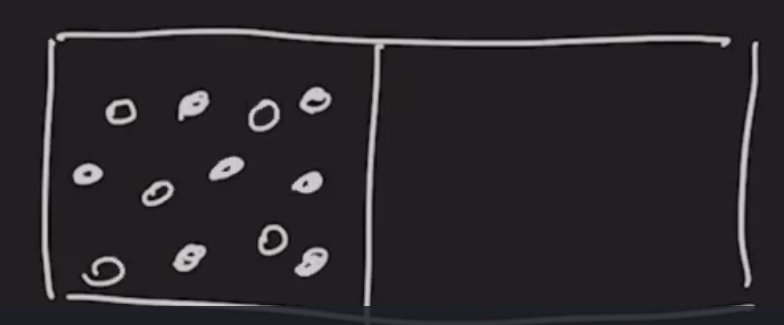
\includegraphics[scale=0.4]{entropy}
	\caption{From Alioscia Hamma's lecture}
\end{figure}


I call that  $ S(\ket{\psi}) = 0$. We call this a quantum gas of non-interacting particles with zero entropy. We want to measure whether the state is in $\ket{+}\bra{+}$ or $\ket{-}\bra{-}$. Well, some of them will be $+$, some will be $-$. well, 
\begin{align}
n_+ = N\abs{w_+}^2 = \f{N}{2} = n_-.
\end{align}
After the measurement, the state will be 
\begin{align}
{\psi} = \abs{w_{+}} P_+ + \abs{w_-}P_- = \abs{w_{+}}\ket{+}\bra{+} + \abs{w_-} \ket{-}\bra{-}.
\end{align}
\textbf{How did the entropy change because of the measurement?} Suppose we have a box like the picture on the right. 
\begin{figure}[!htb]
	\centering
	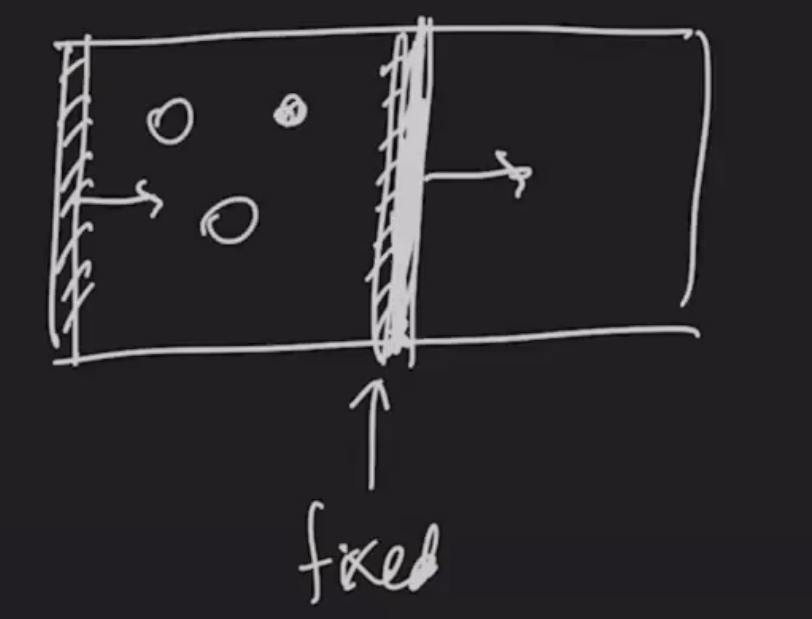
\includegraphics[scale=0.2]{entropy1}
	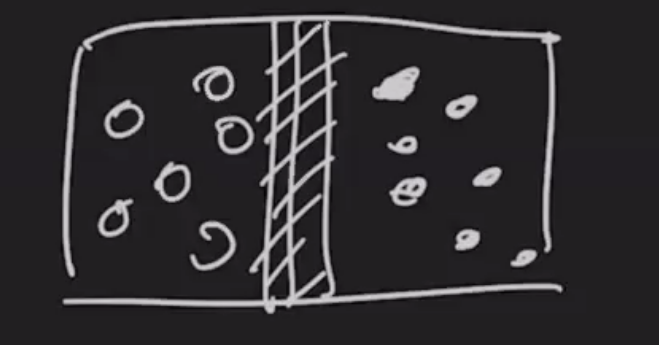
\includegraphics[scale=0.35]{entropy2}
	\caption{From Alioscia Hamma's lecture}
\end{figure}
It has a movable wall on the left and a fixed but semi-transparent wall in the middle. We also have another wall in the middle that can be moved. What Von Neumann thought was that what if we moved both the movable walls so that the volume containing the particles. With the semi-transparent wall, we are left with the picture on the left.\\

Note that nothing happened to the gas, so $Q,W =0$, and everything is reversible. At this point, we have separated the gases, but have not communicated with the environment yet. Now, we do a \textit{isothermal compression}. This is the environment is interacting with our gas. Now, the $+$ gas will be compressed $V \mapsto V'_+ = \abs{w_+}^2 V$, and the $-: V \mapsto \abs{w_-}^2V$. In this compression, the gases exchange work and heat with the environment. What is the entropy exchanged?
\begin{align}
\Delta S^\text{env} = \Delta S_+^\text{env} + \Delta S_-^\text{env}  = -n_+ k \log \f{V'_+}{V} - n_- k \log \f{V'_-}{V}.
\end{align}
Now remember that $n_\pm = \abs{w_\pm}^2N$ and $V_\pm = \abs{w_\pm}^2V$, so 
\begin{align}
\Delta S^\text{env} = -Nk \abs{w_+}^2 \log \abs{w_+}^2-Nk \abs{w_-}^2 \log \abs{w_-}^2.
\end{align}
Now, I do a unitary rotation, $\ket{+}\bra{+} \mapsto w_+\ket{+} + w_-\ket{-}$. This is reversible. Once we've done it for all particles, we're exactly in the initial state. Now, because everything we've done so far is reversible, we have that
\begin{align}
\Delta S^\text{env} + \Delta S^\text{gas} = 0 \implies \Delta S^\text{env} =  - \Delta S^\text{gas} = -(S_1 - S_2) = -S_2.
\end{align}
So, 
\begin{align}
S_2 = Nk \abs{w_+}^2 \log \abs{w_+}^2 + Nk \abs{w_-}^2 \log \abs{w_-}^2.
\end{align}


\begin{defn}[Von Neumann Entropy]
	The entropy of a state $\psi$ is given by
	\begin{align}
	\boxed{S(\psi) = -Nk \sum_i \abs{w_i}^2 \log \abs{w_i}^2}
	\end{align}
\end{defn}

\begin{prop}
	\begin{align}
	S(\bm{1}/d) = \log d
	\end{align}
	\begin{align}
	S_\al = \f{1}{1-\al}\log \Tr(\psi^\al).
	\end{align}
\end{prop}



Let's look at a different definition of Von Neumann entropy, given in Mike and Ike:
\begin{defn}[Von Neumann Entropy]
	The entropy of a quantum state $\rho$ is given by the formula
	\begin{align}
	S(\rho) = -\tr\lp \rho \log \rho \rp.
	\end{align}
	In this formula, the logarithm is take to base two. If $\lambda_x$ are the eigenvalues of $\rho$ then Von Neumann's entropy definition can be re-written as
	\begin{align}
	S(\rho) = -\sum_x \lambda_x \log \lambda_x,
	\end{align}
	where we define $0 \log 0 = 0$. For calculations, it is usually this formula that is most useful. 
\end{defn}


For example, the completely mixed density operator in a $d$-dimensional space, $\bm{1}/d$, has entropy $\log d$, like above. \\


Just for clarity, let's look at the definition of pure states. Pure states are states of the form $\rho = \ket{\psi}\bra{\psi}$. \textbf{Statistical mixtures of pure states form mixed states} of the form $\sum q_j \ket{\psi_j}\bra{\psi_j}$. By definition, pure states are projectors, and thus they are idempotents, i.e., $\rho = \rho^2 = \rho^n$ for any $n\geq 2$. \\


So, just the recap, we know that quantum mechanics  (under the density operator formulation) has \textbf{states}, which are $\psi \geq 0, \tr\psi = 1$, and observables $A = \sum_{ij}A_{ij}\ket{i}\bra{j}$. Next, all Hermitians $\had$ are diagonalizable and the spectral theorem says $\had = \sum_k h_k \ket{\had_k}\bra{\had_k}$ where $\ket{\had_k}\bra{\had_k}$ is a projector and $h_k$'s are the eigenvalues, which are also the possible outcomes. Further, $\psi = \sum_{ij}\psi_{ij}\ket{i}\bra{j} = \sum_k p_k \ket{e_k}\bra{e_k}$. The $p_k$'s here are the eigenvalues of $\psi$. And notice that because $\tr\psi = \sum_k p_k\braket{e_k} = 1$. Thus we have a probability distribution. \\

\begin{defn}[Pure states]
	A state $\psi$ is pure if and only if the probability distribution $p_k$ is extremal, i.e., $(0,0,1,\dots,0)$, i.e., if and only if $\psi = \ket{\psi}\bra{\psi}$ is a rank-1 projector. This is true if and only if $\sum p_k^2 = 1$. The quantity $\sum p_i^2 = \tr(\psi^2)$ is called the \textbf{purity} of the state $\psi$. 
\end{defn}  



The connection with experiments is that, given an operator $A$:
\begin{align}
\Pr(a_i) = \tr\lp \psi \ket{A_i}\bra{A_i} \rp.
\end{align}
Then 
\begin{align}
E[A] = \sum_i \Pr(a_i) a_i = \tr\lp \psi A \rp.
\end{align}
If $\psi$ is pure, then $E[A] = \bra{\psi} A \ket{\psi}$.\\

What happens after measurements? What we learned in QM is that $a_i \mapsto \ket{A_i}$ following a measurement. But what does it mean to say ``if we get $a_i$ we get $A_i$.'' What this really means is that if we measure $a_i$ with probability $\Pr(a_i)$ then we are in $\ket{A_i}$ with probability $\Pr(a_i)$.\\

The act of measurement changes the purity of the state. Suppose we have a pure state $\ket{\psi}$. After measurement, suppose we have $\psi' = \sum_k \Pr(a_i)\ket{A_k}\bra{A_k} = \sum_k \Tr[\psi P_k]P_k$. The state changes -- sometimes called the collapse of the wavefunction. This is due to the fact that $\psi$, before measurement, gives some amplitudes about what potentially can happen. Note that the new state $\psi'$ is a statistical ensemble of pure states $P_k$.\\

So, measurements change the purity of the state. We can ask something like, given a basis $\{ \ket{i}  \}$, what is the operation $D$ that for $X$ nondiagonal, $DX$ is diagonal. This process is called \textbf{dephasing}. What can also ask changes the purity? We can answer the second question: \textbf{entanglement}. 








\newpage

\section{Entanglement}

\textbf{Note:} There is no ``action at a distance.''\\

Now, to define entanglement, we need the notions of ``here'' and ``there.'' Consider a system made up of two parts. The mathematical description is through the tensor product:
\begin{align}
\had = \had_A \otimes \had_B.
\end{align}

Let $A \in \mathcal{B}(\had_A)$ -- $A$ is a bounded operator in $\had(A)$. Suppose $\had_{A} = \text{span}\{ \ket{0},\ket{1}  \}$, and $A = \sum_{i,j\in \{0,1\}}A_{ij}\ket{i}\bra{j}$. Suppose $\had_B = \text{span}\{ \ket{0}_B,\ket{1}_B \}$. Then
\begin{align}
\had = \had_A \times \had_B = \text{span}\{ \ket{00}, \ket{01}, \ket{10}, \ket{11}   \}.
\end{align}
Now, $A \i \mathcal{B}(\had_A)$. Since the original space is $\had = \had_A \otimes \had_B$. To generalize this $A$ so that it acts on the whole of $\had$, we generalize by
\begin{align}
A = \tilde{A} \otimes \Id_B.
\end{align}
With this, with $\psi \in \had$ and $\psi_A \in \had_A$
\begin{align}
E[A] = \tr\lp A \psi \rp = \Tr\lp \tilde{A} \psi_A \rp.
\end{align}
What is $\psi_A$? It turns out that
\begin{align}
\psi_A = \tr_B \psi.
\end{align}
Suppose 
\begin{align}
\ket{\psi} = \lp \f{\ket{0} + \ket{1}}{\sqrt{2}} \rp \otimes \ket{1}.
\end{align}
Then 
\begin{align}
\psi_A &= \Tr_B\psi \nn\\
&= \Tr_B \lb  \lp \f{\ket{0} + \ket{1}}{\sqrt{2}} \rp  \lp \f{\ket{0} + \ket{1}}{\sqrt{2}} \rp^\dagger   \otimes \ket{1}\bra{1} \rb \nn\\
&= \lp \f{\ket{0} + \ket{1}}{\sqrt{2}} \rp    \lp  \f{\bra{0} + \bra{1}}{\sqrt{2}} \rp\nn\\
&= \ket{+}\bra{+}.
\end{align}
Is this a pure state? To check, we compute the purity:
\begin{align}
\psi^2= \ket{+}\bra{+}\ket{+}\bra{+} = \braket{+} = 1,
\end{align}
so $\psi$ is pure. \\

As an exercise we can show that with any \textbf{pure separable state} $\ket{\psi} = \ket{\psi_A}\otimes \ket{\psi_B}$, $\tr_B\psi$ is also a pure state. \\


Next, consider again  $\ket{\psi} = (\ket{01} + \ket{10})/\sqrt{2}$. Is this state pure? The answer is YES because it's already given to us as a ket, i.e., the state is NOT a statistical ensemble of pure states. To show this explicitly, the density matrix is given by
\begin{align}
\psi = \f{1}{2}\lb \ket{01}\bra{01} + \ket{01}\bra{10} + \ket{10}\bra{01} + \ket{10}\bra{10} \rb
\end{align}
then 
\begin{align}
\tr_B\lp \psi \rp = \dots = \f{1}{2}\lb \ket{0}\bra{0}_A + \ket{1}\bra{1}_A \rb.
\end{align}
The purity of this is 
\begin{align}
\tr(\psi^2) = \sum_i p_i^2 = \f{1}{4} + \f{1}{4} \neq 1.
\end{align}
So $\tr_B\psi$ is no longer pure. Thus, \textbf{tracing out sometimes changes the purity}. 

\begin{defn}[Purity and Entanglement]
	We say that if the reduced/marginal state is pure then the original state is also pure. If the reduced/marginal state is not pure then the original state is entangled. 
\end{defn}

This is the essence of entanglement. There is no action at a distance. Rather, this is just an update in our probability distribution. \\




Now, something is still missing here. In physics, we're usually given interactions, not just states and operators. The next thing to learn is time evolution. Let's do that



\newpage

\section{Time evolution}

Let a Hermitian $H \in \mathcal{B}(\had)$ be given. Then the time evolution of $\psi$ is given by
\begin{align}
\psi \mapsto e^{-iH t}\psi e^{iH t}.
\end{align}
For operators, we let the operators evolve, by definition,
\begin{align}
X \mapsto X = e^{iHt}X e^{-iHt}.
\end{align}
Mathematically, this works (the check for why this has to be the case is easy to check). When we compute the expectation value 
\begin{align}
E_t[A] = \Tr\lp A\psi(t) \rp = \Tr\lp A(t)\psi \rb
\end{align}
The term in the middle is the Schrödinger representation, and the term of the RHS is the Heisenberg representation. Next, recall that any unitary can be written as $U = e^{-iHt}$ where $H$ is some Hermitian. This means we can just look at unitaries. With this, the time evolution of $X$ is given by
\begin{align}
U(X) = U^\dagger X U.
\end{align}
This is called the \textit{adjoint action}. Now, a very important property of unitary evolution is that it is \textbf{norm-preserving}, i.e.,
\begin{align}
\norm{U(X)} = \norm{X}.
\end{align}
Recall \textbf{entanglement/ R\'enyi entropy}:
\begin{align}
S_\al = \f{1}{1-\al}\log \Tr(\psi^\al).
\end{align}
Note that the argument of the logarithm looks like the \textbf{purity} of something. Usually, we look at a pure state $\psi$ and look at $\psi_A$. If $\psi_A$ is mixed then $S_\al(\psi_A) \geq 0$. \\

\begin{prop}
	\begin{align}
	S(\psi) = S(\mathcal{U}(\psi)) = S(\mathcal{U}^\dagger \psi \mathcal{U}),
	\end{align}
	i.e., entropy is conserved under unitary evolution. 
\end{prop}

Now, there arises some trouble. We know for a fact that in time, entropy increases by the second law of thermodynamics. But we just claimed that $\mathcal{U}$ preserves entropy. In classical mechanics, we actually have a similar theorem called the \textbf{Liouville Theorem}. This is the problem in statistical mechanics. The rest of this course is targeting this problem.\\



Another interesting thing is ``Chaos.'' In classical mechanics, we have the butterfly effect. In quantum mechanics, consider $\ket{\psi_1}$ and $\ket{\psi_2}$ very close to each other: $\abs{\braket{\psi_1}{\psi_2}} = 1-\epsilon$. Now, 
\begin{align}
\mathcal{U}\ket{\psi_1} = \psi_1(t), \quad \mathcal{U}\ket{\psi_2} = \ket{\psi_2(t)}
\end{align}
It's easy to see that 
\begin{align}
\abs{\bra{\psi_1(t)}\ket{\psi_2}} = 1-\epsilon.
\end{align}
So, there is immunity to small changes in initial condition. \\


Finally, there is a trick to compute purity. Suppose $\psi \in \had$. We want to compute $\Tr \psi^2$. Now, consider the following: Suppose we make a replica, $\psi \mapsto \psi\otimes \psi \i n\had\otimes \had$. Consider the operator $T^{(2)}$ -- a permutation operator of order 2. Let $\{ \ket{i} \}, \{ \ket{j} \}$ be bases of $\had$. Then $\{ \ket{ij} \}$ is a basis for $\had$. $T^{(2)}$ is defined by $\ket{ij} \mapsto \ket{ji}$. Then we can show in the exercise that
\begin{align}
\Tr\psi^2 = \Tr\lb T^{(2)} \psi \otimes \psi \rb.
\end{align}

Next, suppose $\psi$ is pure but $\psi_A$ isn't. What is the purity of $\psi_A$? Well, we want some operator $\mathcal{O}$ such that
\begin{align}
\Tr \psi_A^2 = \Tr\lb \mathcal{O} \psi^{\otimes 2}  \rb?
\end{align}
Again, this will be addressed in the exercises. \\


After these, we will look at how unitary operations make entropies grow. 




   
   
   










\newpage


\section{Quantum Equilibration and Thermalization}

Microscopic laws are time-reversal, but equilibration isn't. So, how are these possible? How can we find the real laws of physics transition from microscopic to macroscopic? We know that unitary microscopic evolution is time-reversal. How do we get non-time-reversal laws in the macroscopic scale? \\

Consider a non-degenerate Hamiltonian $\had = \sum_n E_n P_n = \sum_n E_n \ket{n}\bra{n}$. Why do we make this assumption? Well, why does a Hamiltonian have a degeneracy in the first place? The answer is Noether's theorem. A degeneracy arises when when we evolve the system, some aspects of the system is conserved. An example will be a Hamiltonian with zeros everywhere except for a block on the diagonal. \\

Now, why do we make the assumption that $\had$ is non-degenerate? First, we first note that this assumption is quite strict, because the set of non-degenerate Hamiltonians actually has measure zero! Almost all Hamiltonians are degenerate in some way. We can also have Hamiltonians with degenerate gaps! This is also not very typical of a Hamiltonian. \\

But in any case, we make the non-degenerate assumption to simplify our problems. Okay, so consider the Hamiltonian above. Then recall that $\phi_t = e^{-i\had t}\phi e^{i\had t}$ and $A_t = e^{i\had t}A e^{-i\had t}$. We define
\begin{align}
A_t = \sum_n p_n \bra{n}A \ket{n}  =\Tr\lb A \phi_t \rb = \Tr \lb A_t \phi \rb.
\end{align}
We have the second equality because of the commuting nature of the trace. This is also the relationship between the Schroedinger picture and Heisenberg picture. 

\subsection{Equilibration}

\begin{defn}[Equilibration]
	\begin{align}
	\lim_{t\to \infty}\U_t \phi = \lim_{t\to \infty} e^{-i\had t} \phi e^{i\had t} = \phi_{eq}
	\end{align}
	if equilibration happens. 
\end{defn}

$\phi_{eq}$ is called the steady state, a state that is the fixed point of our unitary evolution:
\begin{align}
\U \phi = \phi.
\end{align}
This means $\phi$ is firstly an eigenstate. So, if $\phi$ is $\ket{E_n}$ then it is an eigenstate. In fact, a steady state need not be an eigenstate. It turns out that $\phi_{eq}$ can, for example, be a Gibbs state:
\begin{align}
\phi = \f{e^{-\beta \had}}{\mathcal{Z}}.
\end{align}
This state does not change in time if \textbf{it commutes with the Hamiltonian}:
\begin{align}
\dot{\phi} = \f{d}{dt}\phi_t  =\dots =-i[\phi,\had] = 0.
\end{align}
So, \textbf{steady states are functions of the Hamiltonian}, or, more generally, a probability distribution over the eigenstates. \\

Now, we want to answer the question whether equilibration is possible? The short answer is NO, because of time reversal. In other words, consider a pure state $\ket{\psi}$. Suppose it evolves to the Gibbs state. This state is no longer pure because the probability distribution is no longer extremal. This means equilibration via unitary evolution is not possible in general. \\

How do we show this rigorously? Consider the distance: 
\begin{align}
\lim_{t\to \infty}\norm{\phi_t - \phi_{eq}} =0
\end{align}
if equilibration is possible. Now, by definition, 
\begin{align}
\lim_{t\to \infty}\norm{\U_t\phi - \U_t\phi_{eq}} =0,
\end{align}
since $\U_t \phi_{eq} = \phi_{eq}$. So, 
\begin{align}
\lim_{t\to \infty}\norm{\U_t\phi - \U_t\phi_{eq}} = \norm{\phi - \phi_{eq}} =0.
\end{align}
This happens if and only if $\phi = \phi_{eq}$ to begin with. This shows that equilibration in quantum mechanics is not possible. But equilibration DOES happen! So how does equilibration happen? \\

What we're forgetting when looking at time evolution of quantum systems so far isn't the full Hamiltonian! We're forgetting the environment, which has its own Hamiltonian. Consider the following: $\phi = \phi_{env}\otimes \phi_{sys}$ obeying the Hamiltonian $\had = \had_{env} + \had_{sys} + \had_{int}$ where $\had_{int}$ is the interaction Hamiltonian. Then 
\begin{align}
\psi_{sys}(t) = \tr_{env}\psi(t) = \tr_{env}\lp \U_t \phi_{sys} \otimes \psi_{env} \rp
\end{align}
Note that $\psi$ is not entangled, but $\psi_{sys}(t)$ can be an entangled state. Now since tracing out is not purity-non-preserving operation, this corresponds to a evolution that is not unitary!  


\subsection{Thermalization: Turtles All The Way Down!}

A small system thermalizes in some bath, which thermalizes in a larger bath, and so on. So, to avoid problems, we will restrict ourselves to unitary time evolution and closed systems. What do we do to get unstuck? We want just the small system to equilibrate. But we also know that $\phi_t$ never equilibrates! What are we missing?\\

The way out is to change our way of thinking. We should not think of $\phi$ are a ``thing'' that equilibrates. Rather, we should look at how expectations $\langle A_t\rangle = \tr[A \phi]$ equilibrate! We should always think about observables, because these are things we can observe! So now, the question becomes whether $\langle A_t\rangle$ can equilibrate.  

\begin{thm}[Von Neumann]
	$\langle A_t\rangle$ is quasi-periodic, and so $\lim_{t\to\infty} A_t$ does not exist.  
\end{thm}

\begin{figure}[!htb]
	\centering
	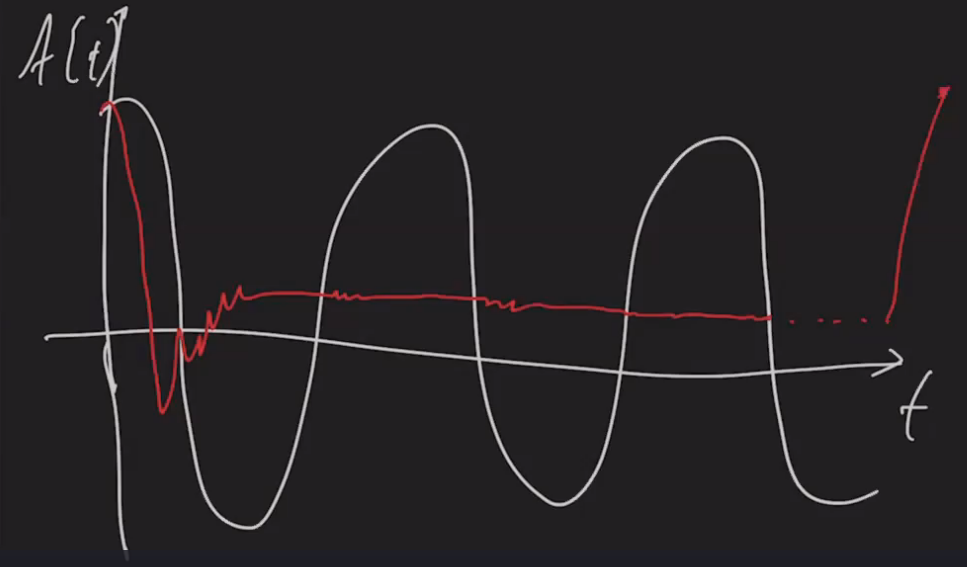
\includegraphics[scale=0.3]{quasi}
\end{figure}

Almost always we're very close to the ``equilibrium'' value, even though $\langle A_t\rangle$ (red) is quasi-periodic. So, consider 
\begin{align}
\Pr[\abs{A_t - A_{eq}} > \epsilon] \ll 1.
\end{align} 
This is called equilibration in probability, or that $A_t$ has typical values $\sim A_{eq}$. Now, what is $A_{eq}$? How do we compute the typical values of $A_t$? 
\begin{figure}[!htb]
	\centering
	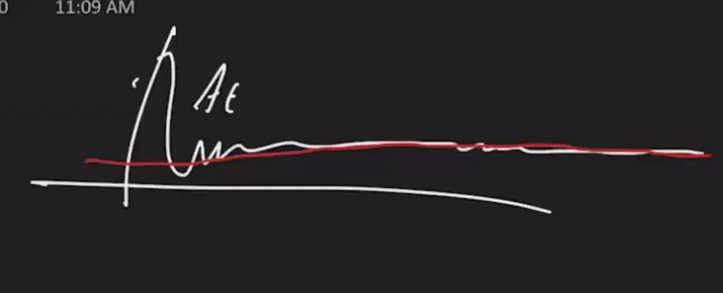
\includegraphics[scale=0.3]{typical}
\end{figure}

Intuitively, it makes sense to define $A_{eq}$ as the time average: 
\begin{align}
A_{eq} = \bar{A} = \lim_{T\to \infty}\f{1}{T}\int^T_0 A_t \,dt.
\end{align}
It turns out that
\begin{align}
A_{eq} = \bar{A} = \tr\lp A \bar{\phi} \rp.
\end{align}
This means the \textbf{typical} value of $A_t$ depends on $\bar{\phi}$.\\

Okay, but notice that $A_t$ is quasi-periodic, which means it has to go back to its initial value at some point:
\begin{figure}[!htb]
	\centering
	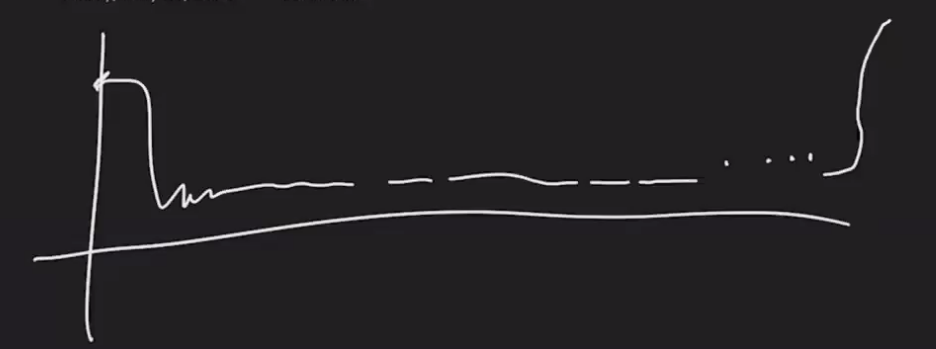
\includegraphics[scale=0.3]{quasi2}
\end{figure}
Right, but we want, also, that the probability that $A_t$ returns to its initial value is small. This, of course, depends on the probability that $\phi_t$ returns to $\phi$, which is 
\begin{align}
\overline{\abs{\braket{\phi}{\phi_t}}}
\end{align} 
This is called the \textbf{return probability}, or the \textbf{Loschmidt echo}.       \\

Now, just to summarize. So far,  we have seen that if our quantum system is open then time evolution is unitary. And if the time evolution is unitary then the quantum system does not reach an equilibrium state. And so the only thing that is compatible with QM is that time average-expectation values equilibrate in probability. In other words, $A_t \to \bar{A}$ in probability, i.e., 
\begin{align}
\Pr(\abs{A_t - \bar{A}} > \ep) \ll 1.
\end{align}
If we can ensure this can happen then it is enough. Now,
\begin{align}
\bar{A} = \Tr[A \bar{\phi}]
\end{align}
with
\begin{align}
\bar{\phi} = \sum_n P_n \phi P_n
\end{align}
where $\had = \sum_n E_n P_n$. We call $\bar{\phi}$ the \textbf{dephasing} in the basis of $\had$:
\begin{align}
D_\had \phi = \bar{\phi}.
\end{align}
$D_\had$ basically erases all the off-diagonal elements of $\phi$. The resulting quantity has matrix elements $\phi_{kk} = p_k = \abs{\braket{\phi}{E_n}}^2$. \\

Now, recall the Loschmidt echo:
\begin{align}
\lag_t = \abs{\braket{\phi}{\phi_t}}^2.
\end{align}
In the exercise, we show that 
\begin{align}
\overline{\lag_t} = \tr \bar{\phi}^2 = \tr\lb\lp D_\had \phi \rp^2 \rb.
\end{align}
which is the purity of $D_\had \phi$. If $\phi$ is pure then $\tr \phi^2 = 1$. Then $\Tr \bar{\phi}^2 = \sum_k p_k^2 \neq 1$. So, $D_\had \phi$ is no longer pure. Is something fishy going on? From $\phi \to \phi_t$ are use a unitary operator, so the purity remains the same. The change is purity is due to the time average, which is not a unitary evolution.\\

$\bar{\phi}$ is NOT an actual state.  So why are we using this state at all? The point of using this fictitious state is so that we get a correct answer: $A_t = \tr[A \phi_t] \to \tr[A\bar{\phi}]$. So, now we would like to understand what makes the fluctuation $\tr[A \phi_t] \approx \tr[A\bar{\phi}]$ small. \\

Since, for pure $\phi$, we have
\begin{align}
\overline{\lag_t} =  \overline{\abs{\braket{\phi}{\phi_t}}^2} = \Tr[\bar{\phi}^2] = p_n^2
\end{align}
which is the probability of going back to $\tr\phi$. Does this probability depend on the initial state $\phi$ or not? The answer is YES, of course. \\

Now, if $\phi$ is not pure then we want to look at the inner product of operators:
\begin{align}
\braket{A}{B} = \Tr[A^\dagger B].
\end{align}
which is just the HS inner product. In this case, the Loschmidt echo becomes
\begin{align}
\lag_t = \abs{\braket{\phi}{\phi_t}}^2 = \Tr[\phi^\dagger \phi_t]. 
\end{align} 

In any case, we showed that, $\bar{\lag_t} = \sum_n p_n^2$ which is just the purity $D_\had \phi$, which depends on $\phi$. 

\begin{exmp}
	Consider $\ket{\phi} = (1/\sqrt{2})(\ket{E_0} + \ket{E_1})$, corresponding to the Hamiltonian $\had = \sum_n E_n \ket{E_n}\bra{E_n}$. Then 
	\begin{align}
	\ket{\phi_t} = \f{1}{\sqrt{2}}\lb e^{-iE_0t}\ket{E_0} + e^{-iE_2t}\ket{E_1} \rb.
	\end{align}
	Then 
	\begin{align}
	\braket{\phi}{\phi_t} = \f{1}{2}\lb e^{-iE_0 t}  + e^{-iE_1t}\rb
	\end{align}
	And so the time average is $1/2$. So this is something with low probability of return, on average.  
\end{exmp}


One can show that if the original state is very spread out in the basis states of the Hamiltonian, then the return probability is very small, which means equilibration occurs very quickly. Now, how likely is it for $\sum_n p_n^2$ to be very small, i.e., $\phi$ is extremely spread out in the basis states of the Hamiltonian? NOT VERY LIKELY! Let's show this mathematically. \\

Consider a random state $\phi$, then we have $\tr((D_h\phi)^2)=  \tr \bar{\phi}^2 = \sum_n p_n^2$.  What is the average of this over all the $\phi$'s what do we get? Well, this is given by
\begin{align}
\boxed{  \la \tr\lb (D_\had \phi)\rb^2  \ra_\phi \equiv \int \tr\lb (D_\had \phi)^2 \rb \,d\phi} 
\end{align}
where of course we require normalization $\int d\phi = 1$. Taking this integral requires knowing the Haar-measure. One can easily prove that
\begin{align}
\la \phi \ra_\phi = \f{\Id}{d}
\end{align} 
which is the microcanonical ensemble. Now to the harder problem. Call $\omega = D_h \phi$. What we want to compute now is 
\begin{align}
\la \tr \omega^2 \ra_\phi.
\end{align}
Now, recall from the exercise to get
\begin{align}
\tr \omega^2 = \tr\lp T^{(2)} \omega^{\otimes 2} \rp.
\end{align}
With this and by linearity we can proceed:
\begin{align}
\la tr\omega^2 \ra &= \la \tr(T^{(2)} \omega^{\otimes 2}) \ra\nn\\
&= \tr \lb T^{(2)} \la \omega^{\otimes 2} \ra \rb\nn\\
&= \tr\lb T^{(2)} \la (D_\had \phi)^{\otimes 2} \ra \rb\nn\\
&= \tr\lb T^{(2)} D_\had^{\otimes 2} \la \phi^{\otimes 2} \ra \rb.
\end{align}
Now, group theory says that
\begin{align}
\la \phi^{\otimes 2}  \ra = \f{\Id_{\had^{\otimes 2}} + T^{(2)}}{d(d+1)}.
\end{align}
Plugging this back into the exercise, we get (in the exercise) $2/(d+1)$. So, the purity of the state after we erase the diagonal elements, on average, is $2/(d+1)$. This means that if the Hilbert space is very large, then the purity is very close to zero. \\


Now, knowing the average of something does not mean much. It might not be the typical case. So is this typical, or does this have a lot of fluctuations, i.e., is the variance of $\bar{\lag}_t$ small or large? What can we say about $\text{Var}(\bar{\lag}_t)$. First, $\bar{\lag}$ is nonnegative. Second, its average is very small. So its variance must also be small. This comes from the \textbf{Markov Inequality}:
\begin{align}
X\geq 0, \Pr(X \geq a) \leq E[X]/a.
\end{align}
We can make $a=1/\sqrt{d}$, so that $\Pr(X \geq 1/\sqrt{d}) \leq 1/\sqrt{d}$. \\

Now, let's consider entanglement. Consider $\had = \had_A \otimes \had_B$ and $\phi$ pure in $\had$. If $\phi$ is entangled then $\tr \phi_A^2 < 1$. Next, recall that $S_2 =  -\log \tr \phi_A^2 $. Now, we ask what $\la -\log \tr \phi_A^2 \ra_\phi$ is, to see how typical entanglement is. Now, 
\begin{align}
\la -\log \tr \phi_A^2 \ra_\phi &\geq -\log \la \tr \phi_A^2 \ra_\phi \nn\\
 &= -\log \la \tr \phi_A^{\otimes 2}  T^{(2)}_A\ra_\phi \nn\\
 &= -\log \tr[T_A^{(2)} \la \phi_A^{\otimes 2} \ra].
\end{align}
In the exercise, we show that 
\begin{align}
\la -\log \tr \phi_A^2 \ra_\phi = \log \f{d_A + d_B}{d_Ad_B+1}.
\end{align}
Now, call the purity $p = \tr \phi_A^2$. Then we show that
\begin{align}
\la p \ra_\phi = \la \tr \phi_A^2 \ra_\phi \f{d_A + d_B}{d_Ad_B+1}.
\end{align} 
Now, if $A$ is our system of interest, then $d_B \gg d_A$ since $B$ is the ``universe'' in this case. But $d_A$ is also quite large by itself, so we have the typical thermodynamic situation: $d_B \gg d_A \gg 1$. With this, 
\begin{align}
\la p \ra_\phi  \approx \f{1}{d_A} = \f{1}{2^{N_A}}.
\end{align}
And so
\begin{align}
\log_2 d_A \geq S_2 \geq \log_2 d_A
\end{align} 
And so, we have that \textbf{almost all states are maximally entangled}.

\newpage

\section{Equilibration}

We introduce the notion of distance between states. 
\begin{align}
d(\rho,\sigma) &= \max_P \abs{\tr P_\rho - \tr P_\sigma} \nn\\
&= \f{1}{2}\norm{\rho - \sigma}_1 \nn\\
&= \f{1}{2}\tr \lb \sqrt{(\rho-\sigma)^\dagger(\rho-\sigma)} \rb.
\end{align}

Consider a map $\Phi$ that is  trace-preserving and maps a state to a state. For example, $\U_t, D_H, \tr_B$ are examples. 

\begin{thm}
	Let a trace-preserving map $\Phi$ be given, then 
	\begin{align}
	d(\Phi(\rho) , \Phi(\sigma)) \leq d(\rho,\sigma).
	\end{align}
\end{thm} 


\begin{thm}
	\begin{align}
	d(\rho_A ,\sigma_A) \leq d(\rho,\sigma).
	\end{align}
\end{thm}

\begin{thm}
	\begin{align}
	\norm{\rho - \sigma}_1 \leq \sqrt{d}\norm{\rho - \sigma}_2 = \sqrt{d \tr (\rho - \sigma)^2}
	\end{align}
\end{thm}


\subsection{Equilibration}

Let $\omega = D_H \phi = \bar{\phi}$ be given and $\omega_S = \tr_B \omega$, with $\had = \had_S \otimes \had_B$. Remember that $A_t \sim \bar{A}$ and $\tr (A\phi_t) \sim \tr A \omega$, and thus we want to show
\begin{align}
\overline{\tr[A \phi_{St}]} \sim \overline{\tr [A \omega_S]}
\end{align}
This means that we want $\overline{d(\phi_{St}, \omega_S)}$ small.

\begin{thm}
	\begin{align}
	\overline{d(\phi_{St},\omega_S)} \leq \f{1}{2}\sqrt{d_S^2 \tr \omega^2}
	\end{align}
	where $\omega = D_H \phi$.
\end{thm} 

\begin{proof}
	We had lemma that says 
	\begin{align}
	d(\rho, \sigma) = \f{1}{2}\tr \sqrt{(\rho - \sigma)^2} \leq \f{1}{2}\sqrt{d\tr (\rho - \sigma)^2}
	\end{align}
	Because $\sqrt{\cdot}$ is concave, we can bring the average inside. So,
	\begin{align}
	\overline{d(\phi_{St}, \omega_S)} \leq \f{1}{2}\sqrt{d_S \overline{\tr(\phi_{St} - \omega_S)^2} }.
	\end{align}
	Now, 
	\begin{align}
	\phi_{St} - \omega_S =  \sum_{k\neq l} c_k c_l^\dagger e^{-i(E_k - E_l)t} \tr_B\ket{E_k}\bra{E_l}.
	\end{align}
	Thus,
	\begin{align}
	\overline{\tr (\phi_{St} - \omega_S)^2} = \sum_{k\neq l, m\neq n}\overline{\tau_{klmn}} \tr \lp \tr_B \ket{E_k}\bra{E_l} \cdot \tr_B \ket{E_m}\bra{E_n}\rp.
	\end{align}
	Explicitly, 
	\begin{align}
	T_{klmn} = c_k c_l^\dagger c_m c_n^\dagger e^{\overline{-i(E_k - E_l + E_m - E_n)t}}. 
	\end{align}
	Now, since we have non-degenerate Hamiltonians, so
	\begin{align}
	\overline{e^{-i()t}} = \delta_{kn}\delta_{lm}.
	\end{align}
	Plug this in to get
	\begin{align}
	\overline{\tr(\dots)^2} &= \sum_{k\neq l} \abs{c_k}^2\abs{c_l}^2 \cdot \tr\lb \tr_B \ket{E_k}\bra{E_l} \cdot \tr_B \ket{E_l} \bra{E_k} \rb \nn\\
	&= \sum_{k\neq l} \tr_B \lp \tr \abs{c_k}^2 P_k  \cdot \tr \abs{c_l}^2 P_l \rp.
	\end{align}
	Now add the $k=l$ terms and subtract them. Recall that
	\begin{align}
	\sum_k \abs{c_k}^2 P_k = \omega
	\end{align}
	so that 
	\begin{align}
	\overline{\tr(\dots)^2} &= \tr_B \omega_B^2 - \sum_k \abs{c_k}^4 \tr \lb \tr_B P_k \rb^2.
	\end{align}
	The term on the right is upper bounded by one. So,
	\begin{align}
	\overline{\tr(\dots)^2} \leq \tr_B \omega_B^2 \leq d_S \tr \omega^2.
	\end{align}
	Plugging everything back in we get
	\begin{align}
	\overline{d(\phi_{St}, \omega_S)} \leq \f{1}{2}\sqrt{d_S^2 \tr \omega^2}
	\end{align}
	so we're done. 
	
\end{proof}


















Typically, $\tr \omega^2 \sim 1/d = 1/(d_Sd_B)$, and so typically, 
\begin{align}
\overline{d(\phi_{St}, \omega_S)} \leq \f{1}{2}\sqrt{d_S/d_B} \ll 1
\end{align}  
because $d_S/d_B \ll 1$. Here ``typically'' is in the sense of the Haar-average. To prove this theorem, we want to compute
\begin{align}
\la \tr\omega^2 \ra_\phi &= \la \tr (D_H \phi)^2 \ra_\phi \nn\\
&= \tr \la (D_H \phi)^{\otimes 2} T^{(2)} \ra_\phi\nn\\
&= \tr  D_H^{\otimes 2} \la  \phi^{\otimes 2}\ra_\phi T^{(2)}  \nn\\
&\sim \f{1}{d}.
\end{align}
So we have that
\begin{align}
\la \overline{d(\phi_{St}, \omega_S)} \ra_\phi \leq \f{1}{2}\sqrt{d_S^2\la \tr \omega^2 \ra}.
\end{align}
From here, we see that $\phi_{St}\sim \omega_S$ almost always. But what is $\omega_S = \tr_B D_H \phi$, typically? We need a new canonical state that doesn't depend on $\phi$ and establish the distance between $\omega_S$ and that state which we will call $\Omega_S$. 

\begin{thm}
	\begin{align}
	\la d(\omega_S, \Omega_S) \ra_\phi \ll 1 
	\end{align}
	where $\omega_S = \tr_B D_H \phi$ and $\Omega_S = \Id_S/d_S$ is the canonical state. 
\end{thm}










\newpage

\section{Resource Theories and Quantum Information}


\newpage
\section{Quantum Thermal Operations}


    



\newpage
\section{Fluctuation Theorems and Quantum Information}


\newpage
\section{Quantum Thermal Machines}




\newpage


\section{Exercises}

\noindent \textbf{1. Density Operators} Show that given the distribution of states $(q_j, \ket{\psi_j})$ the probability of getting an outcome $a_i$ when measuring $A = \sum_i a_i \ket{a_i}\bra{a_i} \equiv \sum_i a_i P_i$ is given by
\begin{align}
\Pr(a_i) = \tr(\psi P_i)
\end{align} 
where we have define the density matrix of the system as
\begin{align}
\psi = \sum_j q_j \ket{\psi_j}\bra{\psi_j}
\end{align}


\begin{proof}
	This is not very hard: 
	\begin{align}
	\Pr(a_i) &= \bra{a_i} \psi \ket{a_i}\nn\\
	&= \sum_j \bra{a_i} q_j \ket{\psi_j}\bra{\psi_j}\ket{a_i}\nn\\
	&= \sum q_j \ket{\psi_j}\bra{\psi_j}\ket{a_i}\bra{a_i}\nn\\
	&= \tr(\psi P_i).
	\end{align}


Alternatively, we can do this like the following: Since the trace is linear, the probability of getting the outcome $a_i$ is 
\begin{align}
\Pr(a_i) = \tr\lb \sum_j q_j \psi_j P_i \rb = \tr\lb \psi P_i \rb.
\end{align}
This is perhaps a better way to do the problem than the previous approach. In any case they're equivalent. 
\end{proof}


\noindent \textbf{2. Partial Trace} Mixed states appear naturally also when considering subsystems of a composite
quantum system. Consider
\begin{align}
A = \tilde{A}_S \otimes I_{\bar{S}}
\end{align}
in a Hilbert space with tensor product structure $\had = \had_S \otimes \had_{\bar{S}}$. It is a natural question to ask what is the state $\rho_S \in \mathcal{B}(\had_S)$ onto the subsystem $\had_S$ that can return all the right expectation values when performing any measurement of operators with that support, namely, the $\tilde{A}_S$. We ask that 
\begin{align}
\tr(A\rho) = \tr(\tilde{A}_S \rho_S).
\end{align}
Show that the solution of this equation is 
\begin{align}
\rho_S = \tr_{\bar{S}}(\rho)
\end{align}
where the operation of partial trace is defined by
\begin{align}
\tr_{\bar{S}}X = \tr_{\bar{S}}\sum_{i_S i_{\bar{S}} j_S j_{\bar{S}}}  X_{i_S i_{\bar{S}} j_S j_{\bar{S}}} \ket{i_S i_{\bar{S}}}\bra{j_S j_{\bar{S}}} = \sum_{i_S  j_S} X_{i_S j_S} \ket{i_S}\bra{j_S}.
\end{align}


\begin{proof}     
	The definition of partial trace above is not very useful due to bad notation. So we will consider an equivalent definition:
	\begin{align}
	\tr_{\bar{S}}(\rho) = \sum_{i_{\bar{S}}} \bra{i_{\bar{S}}}\rho\ket{i_{\bar{S}}}. 
	\end{align}
	Note that this is an operator, not a number.  We want to show
	\begin{align}
	\tr(A\rho) = \tr(\tilde{A}_S \tr_{\bar{S}}(\rho)).
	\end{align}
	Well, by the definition of the trace in terms of the inner product:
	\begin{align}
	\tr(A\rho) &= \tr(\rho A) \nn\\
	&= \tr(\rho(\tilde{A}_S \otimes I_{\bar{S}}) )\nn\\
	&\equiv \tr(\rho (\tilde{A} \otimes I))\nn\\
	&=  \sum_{i_{S}} \sum_{i_{\bar{S}}}\bra{i_{S} i_{\bar{S}}} \rho (\tilde{A}_S \otimes I_{\bar{S}})   \ket{i_{S} i_{\bar{S}}}\nn\\
	&= \sum_{i_{S}} \sum_{i_{\bar{S}}}\bra{i_{S} i_{\bar{S}}} \rho \ket{\tilde{A}_S i_S \otimes  i_{\bar{S}}}\nn\\
	&= \sum_{i_{\bar{S}}}\sum_{i_{S}}  \bra{i_{{S}}}  \bra{i_{\bar{S}}} \rho \ket{i_{\bar{S}}}  \ket{\tilde{A}_S i_S} \nn\\
	&= \tr\lp \tilde{A}_S \tr_{\bar{S}} (\rho) \rp\nn\\
	&= \tr\lp \tilde{A}_S \rho_S \rp.
	\end{align}
	
\end{proof}


\noindent \textbf{3. R\'enyl Entropy} The R\'enyi entropy for R\'enyi index $q$ is defined as
\begin{align}
\boxed{S_q(\rho) = \f{1}{1-q}\log \Tr \rho^q = \f{1}{1-q} \log \lp \sum_i \lambda_i^q \rp}
\end{align} 
where the logarithm is again taken to be base two and $\lambda_i$ are the eigenvalues of $\rho$.

\begin{enumerate}
	\item Show that for the completely mixed density operator $\rho = I/d$ in $d$-dimensional Hilbert space, the von Neumann entropy is given by
	\begin{align}
	S(I/d) = \log d.
	\end{align}
	
	\begin{proof}
		This is very easy. The eigenvalues of $I/d$ are $1/d$. The von Neumann entropy is given as 
		\begin{align}
		S_{vn} = -\sum \lambda_x \log \lambda_x = -\sum \f{1}{d}\log \f{1}{d} = \log d.
		\end{align}
	\end{proof}
	
	\item Show that 
	\begin{align}
	S_0(\rho) =\lim_{q\to 0+} S_q(\rho) =\log (\rank \rho)
	\end{align}
	where $\rank \rho$ is the rank of the density matrix $\rho$.
	
	\begin{proof}
		This is also quite easy. When $q \to 0+$, the definition says the leading factor becomes $+1$. Inside the logarithm, we just get a sum of $\lambda_i^0$. Now, of course these values only approach 1 if they're not zero. So, the sum is exactly the rank of the matrix $\rho$. Thus, 
		\begin{align}
		S_0(\rho) = \log \rank \rho.
		\end{align} 
	\end{proof}
	
	
	\item Show that 
	\begin{align}
	\lim_{q\to 1} S_q(\rho) = S_1(\rho)
	\end{align}
	where $S_1(\rho)$ is the von Neumann entropy. 
	
	\begin{proof}
		This is quite hard. The proof is contained in this \href{https://arxiv.org/pdf/1306.3142.pdf}{\underline{paper}} by Muller-Lennert in 2013. \\
		
		But we can also do this using l'Hopital's rule:
		\begin{align}
		\lim_{q\to 1}S_q(\rho) &= \f{1}{\ln 2}\lim_{q\to 1} \lb \f{\log \lp\sum_i \lambda_i^q\rp}{1-q} \rb\nn\\
		&= \f{1}{\ln 2}\lim_{q\to 1} \lb \f{ \f{1}{\sum_i \lambda_i^q} \sum_i \f{d}{dq} \lambda_i^q}{-1} \rb\nn\\
		&= \f{1}{\ln 2}\lim_{q\to 1}\lb   -\f{\sum_i \lambda_i^q} \sum_i  \lambda_i^q \ln \lambda_i\rb\nn\\
		&= -\f{1}{\sum_i\lambda_i}\sum_i \f{\ln \lambda_i}{\ln 2}\nn\\
		&= -\sum_i \lambda_i \log \lambda_i\nn\\
		&= S_{vn}(\rho).
		\end{align}
	\end{proof}
	
	
	
	
	\item Consider the R\'enyi entropy for the case where the R\'enyi index is an integer $n$ with $n \geq 2$. If $\rho$ corresponds to a pure state, calculate $S_n(\rho)$. Show that if $\rho_\text{pure}$ corresponds to a pure state, then
	\begin{align}
	S_n(\rho_\text{pure}) = 0.
	\end{align}
	
	\begin{proof}
		By definition, pure states are idempotents. This means $\tr(\rho) = \tr(\rho^n) = 1$ always, by normalization. Now, diagonalize $\rho, \rho^2, \dots, \rho^n$ we see that the condition $\tr(\rho^n) = 1$ implies $\sum \lambda_\rho^n = 1$. So, by the definition of the Renyi entropy, we have that 
		\begin{align}
		S_n(\rho_\text{pure}) = 0.
		\end{align}
	\end{proof}
	
	
	
\end{enumerate}




\noindent \textbf{4. Von Neumann Entropy}
Compute the von Neumann entropy of the Gibbs state.


\begin{proof}
	The Gibbs state is given by
	\begin{align}
	\rho = \f{e^{-\beta \had}}{ \tr\lp  e^{-\beta \had} \rp }
	\end{align}
	The von Neumann entropy of $\rho$ is given by
	\begin{align}
	S_{vn}(\rho) = -\sum \lambda_x \log \lambda_x
	\end{align}
	where $\lambda_x$ are the eigenvalues of $\rho$. Suppose the Hamiltonian $\had$ has the spectrum $\{ \sigma_i \}$, then by the spectral mapping theorem we have that the spectrum of $e^{-\beta \had} = \{ e^{-\beta \sigma_i} \}$, and so it follows that
	\begin{align}
	\tr\lp e^{-\beta \had} \rp = \sum e^{-\beta \sigma_i} = \mathcal{Z}
	\end{align}
	where of course $\mathcal{Z}$ is the partition function. With these, the von Neumann entropy is given by
	\begin{align}
	S_{vn} 
	&= -\f{1}{\mathcal{Z}}\sum {e^{-\beta \sigma_i}}\log \f{e^{-\beta \sigma_i}}{\mathcal{Z}} = \log \mathcal{Z} + \beta\langle E \rangle
	\end{align}

	
	
\end{proof}

















\noindent \textbf{5. Swap Operator.} One of the problems of the entanglement entropies is that to know them one has
to know all the eigenvalues of the reduced density operator, which amounts to
knowing the wave-function. In other words, entanglement is not the expectation
value of an observable. Define the swap operator as the operator on two copies of
the original Hilbert space, namely $T^{(2)} \in \had \otimes \had$. This operator is defined from the action on the basis states as
\begin{align}
T^{(2)} \ket{\phi_i \phi_j} = \ket{\phi_j \phi_i}.
\end{align}
\begin{enumerate}
	\item \textbf{Purity as expectation value.} Given a state $\sigma \in \mathcal{B}(\had)$, show that 
	\begin{align}
	\tr\sigma^2 = \tr\lp T^{(2)} \sigma^{\otimes 2} \rp.
	\end{align}
	
	\begin{proof}
		\begin{align}
		\tr\lp T^{(2)}\sigma^{\otimes 2} \rp &= \sum_{i,j} \bra{ij} T^{(2)}\sigma^{\otimes 2} \ket{ij}\nn\\
		&= \sum_{i,j} \bra{ij} T^{(2)} (\sigma \ket{i} \otimes \sigma\ket{j})\nn\\
		&= \sum_{i,j} \bra{ij} T^{(2)} (\sigma \ket{j} \otimes \sigma\ket{i})\nn\\
		&= \sum_{i,j} \bra{ij} \sigma^2 \ket{ji} \nn\\
		&= \sum_i \bra{i}\sigma^2 \ket{i}\nn\\
		&= \tr\lp \sigma^2 \rp.
		\end{align}
	\end{proof}
	
	\item \textbf{Trace of $T^{(2)}$.} Compute the trace of $T^{(2)}$.
	\begin{proof}
		Just use $\sigma = \Id$. Then the $\tr(T^{(2)})$ is just the dimension of the space.  
	\end{proof}
	
	\item \textbf{Frobenius norm.} Show that for any linear operator $X$, the Frobenius norm reads 
	\begin{align}
	\norm{X}_2^2 = \tr\lp T^{(2)} X \otimes X^\dagger \rp.
	\end{align}
	\begin{proof}
		This one is similar to part 1:
		\begin{align}
		\norm{X}_2^2 &= \sqrt{\tr(X^\dagger X)} \nn\\
		&= {\sum_i \bra{i} X^\dagger X \ket{i}}\nn\\
		&= {\sum_{i,j} \bra{i}X^\dagger \ket{i}\bra{j} X\ket{i}   }\nn\\
		&= \sum_{i,j} (\ket{i} \otimes \ket{j})(X^\dagger\ket{j} \otimes X\ket{i})\nn\\
		&= \sum_{i,j} \bra{ij}T^{(2)}( X\ket{i} \otimes X^\dagger\ket{j} )\nn\\
		&= \tr\lp T^{(2)} X \otimes X^\dagger \rp.
		\end{align}
	\end{proof}

\end{enumerate}






\noindent \textbf{6. Unitary Evolution}
\begin{enumerate}
	\item \textbf{Norm invariance.} Show that the Frobenius norm and the Operator norm are preserved by unitary operations.
	\begin{proof}
		This is one easy. For the Frobenius norm, we just use the fact that $\tr(AB) = \tr(BA)$. Everything else follows. In general, things follow from the fact that unitaries preserve the inner product.  
	\end{proof}
	
	\item \textbf{Entropy invariance.} Show that all Entropies are preserved by unitary evolution.
	\begin{proof}
		Entropies depend on something that looks like $\tr \psi^\al$ for some $\al$ and the state $\psi$. Again, because $\tr(BA) = \tr(AB)$, it's an easy argument to show the trace remains invariant.
	\end{proof}

\end{enumerate}



\noindent \textbf{7. Entanglement and partial trace.} Show that, if a state $\sigma(t)$ is evolving in time, the purity of the marginal state $\sigma_A(t)$ is given by 
\begin{align}
\tr \sigma^2_A(t) = \tr \lb T^{(2)} \otimes I_B^{\otimes 2} U^{\otimes 2} \sigma^{\otimes 2} U^{\dagger \otimes 2} \rb
\end{align}
where $U$ is the unitary evolution operator.
\begin{proof}
	To do this we use the identity 
	\begin{align}
	\tr(X_A \rho_A) = \tr\lp X \otimes I_B\rho  \rp
	\end{align}
	then recall that $\sigma(t) = U \sigma U^\dagger$ and take the tensor power two.
\end{proof}



\noindent \textbf{8. Time evolution by Hamiltonian.} Be $\mathcal{U}(X) = e^{iHt} X e^{-iHT} \equiv X_t$ the time evolution generated by a non-degenerate Hamiltonian $H = \sum_n E_n P_n$.
\begin{enumerate}
	\item \textbf{Time averaged operator}
	Define the time average as $\bar{X} = \lim_{T\to \infty} \f{1}{T} \int^T_0 X_t\,dt$. Show that
	\begin{align}
	\bar{X} = \sum_n P_n X P_n.
	\end{align}
\end{enumerate}
\begin{proof}
	This needs quite a lot of manipulations. The key is to expand $X$ in the energy eigenbasis:
	\begin{align}
	\bar{X} &= \f{1}{T}\lim_{T\to \infty}\int_0^T e^{iHt} X e^{-iHT}\,dt\nn\\
	&= \lim_{T\to \infty}\f{1}{T}\int_0^T e^{iE_nt} \sum_{n,m} X_{nm} \ket{n}\bra{m} e^{-iE_mt}\,dt, \quad X_{nm} = \bra{n} X \ket{m}  \nn\\
	&= \lim_{T\to \infty}\f{1}{T}\int_0^T e^{i(E_n-E_m)t} \sum_{n,m} X_{nm} \ket{n}\bra{m}\,dt\nn\\
	&= \braket{n}{m}\sum_{n,m} \ket{n}X_{nm}\bra{m}\nn\\
	&= \braket{n}{m}\sum_{n,m} \ket{n}\bra{n} X \ket{m}\bra{m}\nn\\
	&= \sum_n \ket{n} \bra{n} X \ket{n}\bra{n}\nn\\
	&= \sum_n P_n X P_n.
	\end{align}
	So we're done. 
\end{proof}



\noindent \textbf{9. Quantum Measurement.} Show that, after measuring on the state $\sigma$ some observable $\Omega = \sum_i o_i \ket{i}\bra{i} \equiv \sum_i o_i \omega_i$, the resulting state is 
\begin{align}
\sigma' = \sum_i \omega_i o_i \omega_i.
\end{align}
\begin{proof}
	Well, measurement is basically a projection:
	\begin{align}
	\sigma' &= \sum_i \ket{i}\bra{i}\sigma \nn\\
	&= \sum_i \ket{i}\bra{i}\sum_j \sigma_j \ket{i}\bra{j}\nn\\
	&= \sum_{i,j}\ket{i}\bra{i} \ket{j} \sigma_j \bra{j}\nn\\
	&= \sum_i \ket{i} \sigma_i \bra{i}\nn\\
	&= \sum_i \ket{i} \bra{i} \sigma \ket{i}\bra{i}\nn\\
	&= \sum_i \omega_i \sigma \omega_i
	\end{align}
	where we have used the fact that the matrix element $\sigma_i = \sigma_{ii} = \bra{i}\sigma\ket{i}$.
\end{proof}

  















\noindent \textbf{10. Time averages by Hamiltonian evolution.} Be $\mathcal{U}(X) = e^{iHt} X e^{-iHt} \equiv X_t$ the time evolution generated by a non-degenerate Hamiltonian $H = \sum_n E_n P_n$ and $\phi_t = \mathcal{U}\phi = e^{-iHt}\phi e^{iHt}$ the time evolved state. Let $p_n$ be the probability of being in the state $P_n$, namely $p_n = \tr(\phi P_n)$. 

\begin{itemize}
	\item \textbf{Time averaged state.} Let $\phi$ be a pure state with amplitudes $\ket{\phi} = \sum_n a_n \ket{E_n}$. Show that   
	\begin{align}
	\bar{\phi} = \sum_n P_n \phi P_n = \sum_n p_n P_n = \sum_n \abs{a_n}^2 P_n = D_H \phi
	\end{align}
	and compute its purity. 
	
	\begin{proof}
		 Well, we have already shown that $\bar{\phi} = \sum_n P_n \phi P_n$ earlier. So we only need to verify the subsequent equalities:
		 \begin{align}
		 \bar\phi &= \sum_n P_n \phi P_n \nn\\
		 &= \sum_n \ket{n}\bra{n}\phi P_n\nn\\
		 &= \sum_n \ket{n} \bra{n}\sum_m a_m^\dagger a_m \ket{m}\bra{m} P_n\nn\\
		 &=  \sum_n  \sum_m a_m^\dagger a_m \ket{n} \braket{n}{m}\bra{m} P_n\nn\\
		 &= \sum_n  \sum_m a_m^\dagger a_m \ket{m} \bra{m} P_n\nn\\
		 &= \sum_n  \sum_m a_m^\dagger a_m P_m P_n.
%		 &= \sum_n \tr(\phi P_n)P_n\nn\\
%		 &= \sum_n p_n P_n.
		 \end{align}
		 Now note that $P_m P_n = P_n \delta_{mn}$, so we get $=\sum_n \abs{a_n}^2P_n$ for free. With this we're done. The equality with $D_H \phi$ can readily be checked using its definition. Finally,
		 \begin{align}
		 \tr(\phi P_n) = \tr\lp \sum_n \abs{a_m}^2 P_m  P_n \rp =  \abs{a_n}^2.
		 \end{align}
		 So we're done. The purity in this case is 
		 \begin{align}
		 \tr\lp \bar{\phi}^2 \rp = \sum_n \abs{p_n}^2.
		 \end{align}
	\end{proof}
	
	
	
	\item \textbf{Average Loschmidt Echo.} Define the Loschmidt echo as $\lag_t = \abs{\braket{\phi}{\phi_t}}^2$. Show that $\bar{\lag_t} = \Tr \bar{\phi}^2$.
	
	
	\begin{proof}
		Well, just crank:
		\begin{align}
		\overline{\lag_t} &= \lim_{T\to \infty}\f{1}{T}\int^T_0 \braket{\phi}{\phi_t}\braket{\phi_t}{\phi}\,dt\nn\\
		&= \lim_{T\to \infty}\f{1}{T}\int^T_0 dt\, \lb \sum_n a_n^\dagger \braket{E_n}{e^{-iHt}\phi e^{iHt}}  \rb \times \text{c.c.}\nn\\
		&= \lim_{T\to \infty}\f{1}{T}\int^T_0 dt\, \lb \sum_n \sum_m a_n^\dagger a_m \braket{E_n}{E_m} e^{-i(E_n - E_m)t}  \rb \times \text{c.c.}\nn\\
		&= \sum_{n,m} a^\dagger_n a_n a_m^\dagger a_m\nn\\
		&= \tr  \lp \sum_n a_n^\dagger a_n \ket{n}\bra{n} \sum_m a_m^\dagger a_m\ket{m}\bra{m} \rp \nn\\
		&= \tr \lp \lb \sum_n \abs{a_n}^2 P_n \rb^2  \rp   \nn\\
		&= \tr(\bar{\phi}^2).
		\end{align}
		In the case of mixed states, we can define the Loschmidt echo as
		\begin{align}
		\Tr(\phi^\dagger \phi_t)
		\end{align}
		where $\phi$ and $\phi_t$ are now operators. 
	\end{proof}
	
	
	\item \textbf{Typicality in time (Challenge).} Be $H$ a non-degenerate Hamiltonian with also non-degenerate gaps. Define $\omega = D_H \phi$. Show that 
	\begin{align}
	\overline{D(\phi_{St}, \omega_S)} \leq \f{1}{2}\sqrt{d_S^2\tr \omega^2}.
	\end{align}
	
	
	\begin{proof}
		We'll wait until the next lecture to do this. For now we don't know what the subscript $S$ stands for. 
	\end{proof}
	
	
	
	
	
	
\end{itemize}




\noindent \textbf{11. Average in $\had$}.

\begin{itemize}
	\item \textbf{Haar-average Loschmidt Echo.} Show that
	\begin{align}
	\langle \bar{\lag}_t \rangle_\phi = \f{2}{d+1}.
	\end{align}
	
	
	\begin{proof}
		Well in lecture we have shown that
		\begin{align}
		\la \bar{\lag}_t \ra_\phi 
		&= \tr\lb T^{(2)} D_\had^{(2)} \f{\Id^{\otimes 2} + T^{(2)} }{d(d+1)} \rb \nn\\
		&= \f{1}{d(d+1)}\lb \tr\lb T^{(2)} \lb D_\had^{\otimes 2} \Id^{\otimes 2} + \D_\had^{\otimes 2} T^{(2)}  \rb \rb \rb.
		\end{align}
		Now, 
		\begin{align}
		D_\had^{\otimes 2} \Id^{\otimes 2} = \sum_{k}P_k \Id P_k = \sum_k P_kP_k = \sum_k P_k = \Id^{\otimes 2}. 
		\end{align}
		And,
		\begin{align}
		D_\had^{\otimes 2}T^{(2)} &= \sum_{n,m} \ket{nm}\bra{nm} T^{(2)} \ket{nm}\bra{nm}\nn\\
		&= \sum_{n,m} \ket{nm}\braket{nm}{mn}\bra{nm}\nn\\
		&= \sum_{n} \ket{nn}\bra{nn} \nn\\
		&\implies \tr (D_\had^{\otimes 2} T^{(2)}) = d. 
		\end{align}
		With these, we can continue:
		\begin{align}
		\la \bar{\lag}_t \ra_\phi 
		&= \tr\lb T^{(2)} D_\had^{(2)} \f{\Id^{\otimes 2} + T^{(2)} }{d(d+1)} \rb \nn\\
		&= \f{1}{d(d+1)}\lb \tr\lb T^{(2)} \lb D_\had^{\otimes 2} \Id^{\otimes 2} + \D_\had^{\otimes 2} T^{(2)}  \rb \rb \rb\nn\\
		&= \f{1}{d(d+1)}\lb \tr\lb T^{( 2)} \rb + d \rb\nn\\
%		&= \f{2}{d(d+1)}\tr\lb T^{\otimes 2} \rb\nn\\
		&= \f{2}{d(d+1)}d \nn\\
		&= \f{2}{d+1}
		\end{align}
		where we have used the fact that the original Hilbert space is $d$-dimensional. Using an identity we saw earlier, we can show that $\tr(T^{(2)}) = d$. With this we're done. 
	\end{proof}
	
	
	\item \textbf{Markov Inequality.} Use Markov inequality to upper bound
	\begin{align}
	\langle \Pr(\abs{A_t - \bar{A}} > \epsilon)\rangle_\phi
	\end{align}
	
	
	\begin{proof}
		to be continued...
	\end{proof}
	
	\item \textbf{Haar-average purity.} Show that
	\begin{align}
	\langle \tr \phi_A^2 \rangle_\phi = \f{d_A + d_B}{d_A d_B + 1}.
	\end{align}
	
	
	\begin{proof}
		This is a generalization of the first item. To avoid running into trouble with $\tr^{\otimes 2}$, we use the identity
		\begin{align}
		\phi_A^2 = \tr_A (T^{(2)} \phi_A^{\otimes 2}) =  \tr   T^{(2)} \otimes \Id_B  \phi^{\otimes 2}.
		\end{align}
		With this, 
		\begin{align}
		\la \tr \tr T^{(2)} \otimes \Id_B  \phi^{\otimes 2}  \ra_\phi &= \tr \tr \la T^{(2)} \otimes \Id_B \phi^{\otimes 2} \ra_\phi \nn\\
		&= \tr \tr  T^{(2)} \otimes \Id_B \la \phi^{\otimes 2} \ra_\phi \nn\\
		&= \tr \tr T^{(2)} \otimes \Id_B \f{\Id_{A\otimes B} + T^{(2)}}{d_A d_B(d_A d_B + 1)} \nn\\
		&= \f{d_A d_B(d_A + d_B)}{d_Ad_B(d_A d_B  + 1)}\nn\\
		&= \f{d_A + d_B}{d_A d_B + 1}.
		\end{align}
	\end{proof}


	\item \textbf{Purity of the dephased state.} Let $\omega = D_\had \phi$. Show that 
	\begin{align}
	\la \tr \omega^2 \ra_\phi < \f{2}{d}.
	\end{align}
	
	\begin{proof}
		Well we have that $\omega = \bar{\phi} = D_H \phi$. As we have seen, $\tr \omega^2 = \tr \bar{\phi}^2 = \bar{\lag}_t$ with the property
		\begin{align}
		\la \bar{\lag}_t \ra_\phi = \f{2}{d+1} < \f{2}{d}. 
		\end{align}
	\end{proof}




	\item \textbf{Typicality of canonical state (challenge).} Define $\omega = D_H \phi$. Also define $\Omega_S \equiv \la \tr_B \Omega \ra_\phi = \la \omega_S\ra_\phi$. Be $d(\cdot,\cdot)$ the trace distance. Show that
	\begin{align}
	\langle d\lp \omega_S, \f{\Id_S}{d_S} \rp \rangle_\phi \leq \f{1}{2}\sqrt{\f{1}{d_B}}
	\end{align}
	
	\begin{proof}
		to be continued... 
	\end{proof}



	\item \textbf{General canonical state.} Consider a subspace $\had_R \subset \had$ and let $\prod_R$ the projector on it. If we take the Haar average on $\had_R$ one has
	\begin{align}
	\la \phi^{\otimes 2}\ra_\phi = \f{\prod_R^{\otimes 2} (\Id^{\otimes 2} + T^{(2)})}{d_R (d_R+1)}
	\end{align}
	Then show that, in this subspace, the bound of the previous exercise holds as
	\begin{align}
	\langle d\lp \omega_S, \f{\Omega_S}{d_S} \rp \rangle_\phi \leq \f{1}{2}\sqrt{\f{d_S}{d_R}}
	\end{align}
	Also show that, in the same subspace, the bound on the Haar-average purity reads
	\begin{align}
	\la \tr \omega^2 \ra_\phi < \f{2}{d_R}.
	\end{align}
\end{itemize}






    










\newpage
\chapter{Numerical Methods \& Condensed Matter Physics}

\textbf{Instructor:} Aaron Szasz\\

This course has two main goals: (1) to introduce some key models from condensed matter physics; and (2) to introduce some numerical approaches to studying these (and other) models.  As a precursor to these objectives, we will carefully understand many-body states and operators from the perspective of condensed matter theory.  (However, I will cover only spin models.  We will not discuss or use second quantization.)\\



Once this background is established, we will study the method of exact diagonalization and write simple python programs to find ground states, correlation functions, energy gaps, and other properties of the transverse-field Ising model and XXZ model.  We will also discuss the computational limitations of exact diagonalization.  Finally, I will introduce the concept of matrix product states, and we will see how these can be used with algorithms such as the density matrix renormalization group (DMRG) to study ground state properties for much larger systems than can be studied with exact diagonalization.


\section{Introduction}

What is \textit{condensed matter}? This is the study of many particles interacting with each other. This could be studying crystals, liquid, etc. These are all condensed matter. We will be studying this using computer programs. \\

The goals of this course are
\begin{itemize}
	\item Learn some numerical methods.
	\item To learn important models in condensed-matter physics.  
\end{itemize}

In particular, we will be studying the quantum Ising model, or equivalently the transverse field Ising model (TFIM) given by the Hamiltonian
\begin{align}
\had = -J \sum_i S^z_i S^z_{i+1} - h \sum_i S^x_i
\end{align}

We will first cover some background material required for the rest of the course. Then, we will look at \textbf{exact diagonalization} and use it to solve the Ising model. On the third lecture, we will continue with \textit{exact diagonalization}, and depending on how much time we have we will study the $XXZ$ model. On the fourth lecture, we will look at \textbf{matrix product states (MPS)}. On the fifth day, we will use MPS to solve the Ising and XXZ models more efficiently than using exact diagonalization.


\newpage
   

%\section{L1: Introduction to many-particle states and operators}




\section{The Ising model: Motivation}

The Ising model is important because it models magnetism and features quantum phase transition, which is an important topic we will cover later.\\

Consider a one-dimensional chain of $N$ atoms. Each atom has one electron, and that the electrons cannot move due to Coulomb repulsion. So, we have 1 fixed electron per site. For each atom, we solve a local SE and get some set of orbitals. \\

We will assume that each electron is in the $p^z$ orbital and forget about it. \\

We note that this description allows for only one degree of freedom, which is the spin of our electron. Two neighboring electrons can have the same or opposite spins. Our model is given by the Hamiltonian
\begin{align}
\had = -J \sum_i S_i^z S_{i+1}^z
\end{align}
the product $S_iS_{i+1}$ is 1 if the electrons are parallel, and $-1$ if antiparallel. When $J > 0$, the model favors all electrons pointing in the same direction. Now, if the model only has an external field
\begin{align}
-h \sum_i S_i^x
\end{align}
which favors all electrons point in the direction of the external field $+x$. \\

The goal is, given the Hamiltonian:
\begin{align}
\had = -J \sum_i S^z_i S^z_{i+1} - h \sum_i S^x_i
\end{align}
What is the most favorable configuration of the electron?


















\section{Introduction to many-particle states and operators}

\subsection{Spin 1/2 Systems} 

This appears in many introductory quantum mechanics courses, but we'll review this anyway. \\

In general, a state of a spin-1/2 system  can be written as a linear superposition of two spin states
\begin{align}
\ket{\psi} = a\ket{\uparrow} + b\ket{\downarrow}
\end{align}
where $\ket{\psi}$ is normalized and $\ket{\uparrow},\ket{\downarrow}$ form an ONB. This means that $\braket{\uparrow\downarrow} = 1$ and $\braket{\uparrow}{\downarrow} = 0$. 

\subsection{Operators on Spin-1/2 Systems}
An $\mathcal{O}$ is specified by its action on the basis state: 
\begin{align}
\mathcal{O}\ket{\uparrow} = \mathcal{O}_{11}\ket{\uparrow} + \mathcal{O}_{12}\ket{\downarrow},\quad \mathcal{O}\ket{\downarrow} = \mathcal{O}_{21}\ket{\uparrow} + \mathcal{O}_{22}\ket{\downarrow}.
\end{align}
To write in a matrix representation, we will assign $\ket{\uparrow} = (1,0)^\top$ and $\ket{\downarrow} = (0,1)^\top$. With this, we can find operators as well as other states in this basis.\\

An aside: Consider a $2\times 2$ matrix $\mathcal{O} = [O_{ij}]$. Note that $\mathcal{O}(1,0)^\top$ returns the first column of $\mathcal{O}$, and so on. This means any matrix $\mathcal{O}$ can be written as the output of $\mathcal{O}$ when fed the standard basis states. \\

Suppose we want to find the first column of $\mathcal{O}$. From the definition above, we can easily see that
\begin{align}
\mathcal{O} = \begin{bmatrix}
\mathcal{O}_{11} & \mathcal{O}_{12} \\ \mathcal{O}_{21} & \mathcal{O}_{22}
\end{bmatrix}
\end{align}


We care a lot about Hermitian operators: $\mathcal{O} = \mathcal{O}^\dagger$. For $2\times 2$ matrices, any Hermitian operator can be written as 
\begin{align}
\mathcal{O} = a\Id + b\sigma^z + c\sigma^x + d\sigma^y
\end{align}
where $\sigma^i$ are the Pauli matrices. Now, we want to write this in the language of states and operators. Recall that 
\begin{align}
\sigma^z\ket{\uparrow} = \ket{\uparrow}, \quad \sigma^z\ket{\downarrow} = -\ket{\downarrow}
\end{align}
and so on: $\sigma^x$ flips the arrow, and $\sigma^y$ flips and multiplies $\ket{\uparrow}$ by $i$ and $\ket{\downarrow}$ by $-i$. \\

Now, matrices can appear different under different bases. Consider the basis given by
\begin{align}
\ket{+} = \f{1}{\sqrt{2}}\lp \ket{\uparrow} + \ket{\downarrow} \rp = (1,0)^\top, \quad
\ket{-} = \f{1}{\sqrt{2}}\lp \ket{\uparrow} - \ket{\downarrow} \rp = (0,1)^\top
\end{align}
This is an new ONB, by inspection. \\
 
What do the Pauli matrices become under this change of basis? Well, the first column of the new $\sigma^z$ is given by
\begin{align}
\sigma^z\begin{bmatrix}
1\\0
\end{bmatrix}_* = \f{1}{\sqrt{2}} \sigma^z \lp \ket{\uparrow} +  \ket{\downarrow} \rp = \f{1}{\sqrt{2}}\lp \ket{\uparrow} - \ket{\downarrow} \rp  =\ket{-} = \begin{bmatrix}
0\\1
\end{bmatrix}_*
\end{align}
Similarly, we can show that $\sigma^z\ket{\pm} = \ket{\mp}$. In this new basis, $\sigma^z_{new} = \sigma^x$. We can also find the form for the other matrices, but let's not worry about that. The gist is that $\ket{\uparrow\downarrow}$ are the $z$-eigenstates, and $\ket{\leftarrow\rightarrow}$ are the $x$-eigenstates. \\

How the matrices change can be found via the usual change of basis that we all have seen in linear algebra.\\



\section{Tensor Product Spaces}

Suppose there are two space of spin-1/2 particles. The question we want to answer is: What are the allowed states of the 2-spin system? The answer is this: any state in the ``tensor product space,'' which is the vector space whose basis is the following four vectors: $\{ \ket{\uparrow\uparrow}, \ket{\uparrow\downarrow}, \ket{\downarrow\uparrow}, \ket{\downarrow\downarrow}\}$. Each basis vector is an ordered pair, the first being a basis vector in $A$, the second in $B$. \\


So, a general state in the tensor product space is just some superposition of these vectors. What is the inner product in this new space? Suppose we have
\begin{align}
\ket{\psi_A} \otimes \ket{\psi_B}, \quad \ket{\phi_A} \otimes \ket{\phi_B}.
\end{align}
Then the inner product between these is defined as 
\begin{align}
(\bra{\psi_A} \otimes \bra{\psi_B}) (\ket{\phi_A} \otimes \ket{\phi_B}) = \braket{\psi_A}{\phi_A} \cdot \braket{\psi_B}{\phi_B}.
\end{align}


One important consequence is that if the $A$ part is orthogonal or the $B$ part is orthogonal then the inner product in the tensor space is also zero (so, also orthogonal). This is quite easy to see. \\

Finally, we want to know how to apply operators. And operator on the tensor product space looks like
\begin{align}
\mathcal{O} = \sum_i \mathcal{O}^A_i \otimes \mathcal{O}^B_i.
\end{align}
The way each component of $\mathcal{O}$ acts is the following:
\begin{align}
(\mathcal{O}^A \otimes \mathcal{O}^B) (\ket{\psi_A} \otimes \ket{\psi_B}) = (\mathcal{A} \ket{\psi_A}) \otimes (\mathcal{A} \ket{\psi_B}).
\end{align}
By linearity, we can work out how $\mathcal{O}$ acts in general.\\

From this definition, we can see some useful facts. Suppose we want to multiply two operators: 
\begin{align}
(\mathcal{A} \otimes \mathcal{O}^B)(\tilde{\mathcal{O}}^A \otimes \tilde{\mathcal{O}}^B )(\ket{\psi_A} \otimes \ket{\psi_B}) = \dots = (\mathcal{O}^A\tilde{\mathcal{O}}^A \otimes \mathcal{O}^B\tilde{\mathcal{O}}^B)(\psi_A\psi_B).
\end{align}
So, we have
\begin{align}
(O^A \otimes O^B)(H^A \otimes H^B)= O^A H^A \otimes O^B H^B. 
\end{align}

Next, suppose we have $O^A \otimes \Id^B$ and $\Id^A \otimes O^B$. By looking at the commutation, we can easily check that these commute. This fact on be summarized as the following: ``Operators on different sites commute.'' \\


\subsection{Born Rule for Probabilities}

Now we want to look at how to get probabilities. Suppose
\begin{align}
\ket{\psi} = a\ket{00} + b\ket{01} + c\ket{10} + d\ket{00}.
\end{align}
Then $P(00) = \abs{a}^2$, $P(01) = \abs{b}^2$. Then $P(0_A) = \abs{a}^2 + \abs{b}^2$. Finally, suppose we want to find expectation value:
\begin{align}
\langle \sigma^z_A \rangle = \langle \sigma^z_A \otimes \Id_B \rangle = 1\cdot P(0_A) + (-1)P(1_A) = \abs{a}^2 + \abs{b}^2 - \abs{c}^2 - \abs{d}^2.
\end{align}
With this, in the state $\ket{\psi}$, we're going to calculate $\langle \sigma^z_A \otimes \Id_B\rangle $ directly:
\begin{align}
\bra{\dots} \sigma^z_A \otimes \Id_B\ket{\dots} = \dots =  \abs{a}^2 + \abs{b}^2 - \abs{c}^2 - \abs{d}^2
\end{align}
as expected.



\subsection{Expectation Values}

Another useful way to compute expectation values is to use matrix representations. First, we assign basis vectors. Then find matrix for $\sigma_A^z \otimes \Id_B$. Then find matrix/vector representation of $\ket{\psi}$. Finally, multiply out. \\

At this point, we will frequently use the short hand $\ket{\psi_A}\ket{\phi_B} = \ket{\psi\phi}$. With this, we introduce the representation:
\begin{align}
&\ket{\uparrow\uparrow} = (1,0,0,0), \quad \ket{\downarrow\uparrow} = (0,0,1,0)\nn\\
&\ket{\uparrow\downarrow} = (0,1,0,0), \quad \ket{\downarrow\downarrow} = (0,0,0,1)
\end{align}
We want to find the matrix for $\sigma^z_A \otimes  \Id_B$. To do this, we find column-by-column by letting it act on the standard basis vectors. After this is done, we find that 
\begin{align}
(\sigma_A^z \otimes \Id_B) = \begin{bmatrix}
1 &&&\\
& 1 && \\
&&-1&\\
&&&-1
\end{bmatrix}
\end{align}
Finally, we can verify that
\begin{align}
\bra{\psi} \sigma^z_A \otimes \Id_B \ket{\psi} = \abs{a}^2 + \abs{b}^2 - \abs{c}^2 - \abs{d}^2.
\end{align}


\begin{exmp}
	We will look at the $4\times 4$ matrices in this basis for the following operators:
	\begin{align}
	\sigma_A^y \otimes \sigma_B^z = \begin{bmatrix}
	&&-i&\\
	&&&i\\
	i&&&\\
	&-i&&
	\end{bmatrix}
	\end{align}
	
	\begin{align}
	\sigma^z_A \otimes \sigma^y_B = \begin{bmatrix}
	&-i&& \\
	i&&&\\
	&&&i\\
	&&-i&
	\end{bmatrix}
	\end{align}
\end{exmp}

A shortcut to do these calculations is of course the Kronecker product:
\begin{align}
\sigma_A^y \otimes \sigma_B^z = 
\begin{bmatrix}
0 & -i \\ i & 0
\end{bmatrix} \otimes \begin{bmatrix}
1 & 0 \\ 0 & -1
\end{bmatrix}
=\begin{bmatrix}
&&-i&\\
&&&i\\
i&&&\\
&-i&&
\end{bmatrix}
\end{align}

\begin{align}
\sigma^z_A \otimes \sigma^y_B = 
\begin{bmatrix}
1 & 0 \\ 0 & -1
\end{bmatrix} \otimes \begin{bmatrix}
0 & -i \\ i & 0
\end{bmatrix}  
=\begin{bmatrix}
&-i&& \\
i&&&\\
&&&i\\
&&-i&
\end{bmatrix}
\end{align}
In general, 
\begin{align}
A \otimes B = \begin{bmatrix}
a_{11}B & a_{12}B \\ a_{21}B & a_{22}B
\end{bmatrix}.
\end{align}
This is always true if the choice of basis is correct. They are correct in the sense that we can construct the tensor product basis by taking Kronecker products of the basis vectors of the factor space. \\


The moral of the story is this. The matrix for $\mathcal{O}_A \otimes \mathcal{O}_B$ is the Kronecker product of matrices for $\mathcal{O}_A$ and $\mathcal{O}_B$. 






\section{The Two-site Ising Model}

Recall the Hamiltonian for the model:
\begin{align}
\had = -J \sum_i S_i^z S_{i+1}^z - h \sum_i S_i^x.
\end{align}
where
\begin{align}
S_i^z = \f{\hbar}{2}\sigma_i^z.
\end{align}
We can rewrite the model as
\begin{align}
\had = -J \lp \f{\hbar}{2} \rp^2 \sim_i \sigma_i^z \sigma_{i+1}^z - h \f{\hbar}{2}\sum_i \sigma^x_i
\end{align}
Let the constants absorb $\hbar/2, \hbar^2/4$ respectively, then the model becomes
\begin{align}
\had = -J \sum_i \sigma_i^z\sigma_{i+1}^z - h\sum_i \sigma_i^x.
\end{align}
Next, we want to make this precise in the sense of tensor products. For the two-site model, we have precisely
\begin{align}
\had = -J \sigma_0^z \otimes \sigma_1^z - h (\sigma_0^x \otimes \Id_1 + \Id_0\otimes\sigma_1^x).
\end{align} 
We can now convert this into a $4\times 4$ matrix, in the programming exercises. \\

Before any programming though, let's do this by hand. First, let us find the matrix for $\sigma_0^z \otimes \sigma_1^z$. Once we do that, we will find the eigenstates and the eigenvalues of $H$ when $h=0$. Furthermore, we will show that in each of the eigenstate, $\langle \sigma_0^x\otimes \Id_1 + \Id_0 \otimes \sigma_1^x \rangle = 0$. Next, we will do the opposite find the matrix for $\sigma_0^x\otimes \Id_1 + \Id_0 \otimes \sigma_1^x$. Find the eigenvalues and eigenvectors when $J =0$. Then, we will show that in each of these states, $\langle \sigma_0^z \otimes \sigma_1^z \rangle = 0$. Then, we will find the $4\times 4$ matrix for $\had$. \\

Well,
\begin{align}
\sigma^z \otimes \sigma^z = \text{diag}(1,-1,-1,1).
\end{align} 
Obviously the eigenstates are exactly the vectors in the $ZZ$ basis: $\{ \ket{00}, \ket{01}, \ket{10}, \ket{11}\}$ with eigenvalues $1,-1,-1,1$ respectively. The corresponding eigenvalues in the Hamiltonian are $-J,J,J,-J$. \\

Next, to see that $\langle \sigma_0^x\otimes \Id_1 + \Id_0 \otimes \sigma_1^x \rangle = 0$ for each eigenvector, just use the fact that $\sigma^z\ket{\uparrow} = \ket{\downarrow}$ and $\sigma^x\ket{\downarrow} = \ket{\uparrow}$ and that the inner product $\braket{\uparrow}{\downarrow} = 0$. This part is easy.\\

Next, 
\begin{align}
\sigma_0^x\otimes \Id_1 + \Id_0 \otimes \sigma_1^x = \begin{bmatrix}
\sigma^x & \Id \\ \Id & \sigma^x
\end{bmatrix}.
\end{align}

The eigenvectors in this case will be $\{ \ket{++}, \ket{-+}, \ket{+-}, \ket{--}  \}$. The eigenvalues are $\{1,0,0,-1\}$ respectively. These correspond with th eigenvalues $-2h,0,0,2h$ in the Hamiltonian. Verifying the expectation is easy, so again I won't do that.\\

Finally, the $4\times 4$ matrix for $H$ is given by
\begin{align}
\had = -J\begin{bmatrix}
1&&&\\&-1&&\\&&-1&\\&&&1
\end{bmatrix} - h\begin{bmatrix}
&1&1&\\1&&&1\\1&&&1\\&1&1&
\end{bmatrix} = \begin{bmatrix}
-J&-h&-h&\\-h&J&&-h\\-h&&J&-h\\&-h&-h&-J
\end{bmatrix}
\end{align}

We will solve this and $n$-site Ising models next. First, we want to find the eigenstate energies for any $J,h$ and some properties of the ground state (GS). To do this, we use programming. To find properties of the ground states, we want to find expectation values. For example, we want to find $\langle \sigma^z_0 + \sigma_1^z \rangle $, which is the tendency of spins to point along $z$ in a particular direction. We can also look at $\langle \sigma_0^z \otimes \sigma_1^z \rangle$ which is the tendency of the two spins to point parallel along $z$. 

\begin{defn}[Correlation Function]
	The quantity $\langle \mathcal{O}_A \mathcal{B}\rangle$ is called a correlation function. 
\end{defn}

Before we start, we note that $\had$ has two parameters $J$ and $h$. But by the form of $\had$ we can scale things to that it only has one parameter $g = h/J$, which is the relative strength factor. This is nice if we want to solve the model for every parameter point. Varying one parameter is much better than two. With this, we will solve
\begin{align}
\had = -\sigma^z_0 \otimes \sigma_1^z  - g\lp \sigma_0^x\otimes \Id_1 + \Id_0 \otimes \sigma_1^x \rp.
\end{align}

Here's what we get:
\begin{figure}[!htb]
	\centering
	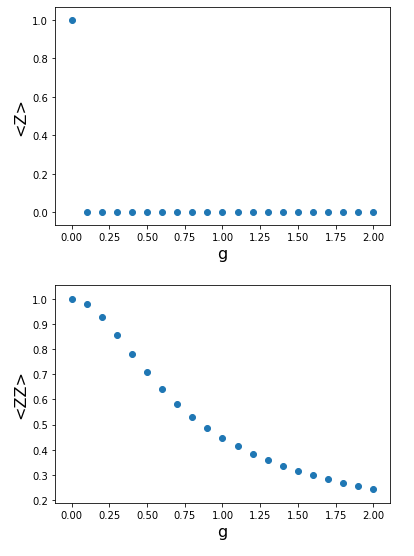
\includegraphics[scale=0.5]{ising1}
	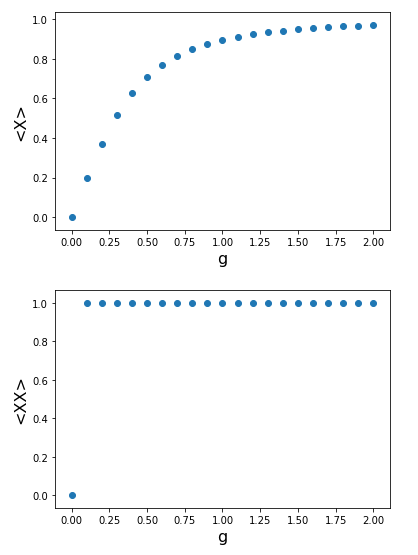
\includegraphics[scale=0.5]{ising2}
\end{figure}

We see jumps in $\langle Z \rangle = \langle \sigma^z_0 + \sigma^z_1\rangle/2$ and $\langle \sigma^x\otimes \sigma^x\rangle$. Why is that? Let's start with the first one. We ask two questions: why is it zero and why does it jump from 1 to 0? When $g=0$, there are two possible ground states $\uparrow\uparrow$ and $\downarrow\downarrow$. This means the ground state looks like $\ket{\psi} = a\ket{\uparrow\uparrow} + b\ket{\downarrow\downarrow}$. The expectation value $\langle \sigma_0^z + \sigma_1^z \rangle/2$ in this case will be $(\abs{a}^2 - \abs{b}^2)$. This means we'll get a random answer at $g=0$. Python randomly picks $a,b$ when it does the numerical calculation for the eigenvalues. This means the $g=0$ value is meaningless. Now, when $g\neq 0$, then because the eigenstates respect the symmetries of the Hamiltonian, when we flip all spins, the Hamiltonian doesn't change. This means the ground state has $\ket{\uparrow}$ and $\ket{\downarrow}$ parts that are equal. In comparison, $\langle \sigma^z \otimes \sigma^z$ is a better measure of the tendency of spins to point along $z$. \\

The case with $x$ occurs for the same reason. $\sigma^x\otimes \sigma^x$ has $z-y$ symmetry where we get a degeneracy in the eigenvalues. But we also note that $\langle \sigma^x \otimes \sigma^x\rangle$ is constant, which means $[\had,\sigma^x \otimes \sigma^x ]=0$, which says that $\sigma^x \otimes \sigma^x$ is a conserved quantity.  









\section{The $N$-site Ising Model:}

The Hamiltonian is given by
\begin{align}
\had/J =-\sum_i \sigma_i^z \sigma_{i+1}^z - g \sum_i \sigma_i^x. 
\end{align}

We want to solve this model. To do this, we need to write the matrix for the Hamiltonian. We follow the steps below:
\begin{itemize}
	\item Find a basis. 
	\item Find a matrix for $\had$
	\item Find the ground state
	\item Calculate expectation values, especially $\langle ]sigma_0^z \otimes \sigma_{N-1}^z$.
\end{itemize}

With $N$ sites, we have $2^N$ basis states. Let's pick the standard basis states as the basis for the space, where $(1,0,\dots,0)^\top = \ket{\uparrow\dots\uparrow} = \ket{0}_{2^N-1}$ and so on. Now, we need a function to turn the index (0,1,2,...) into the list of spins. Suppose that $N=3$. Then we can use binary arithmetics to get back the list of spins. \\

Now how do we find the matrix $\had$? There are a few methods to do this:
\begin{itemize}
	\item \textbf{Kronecker product:} Suppose we want to do the following $\sigma_0^x \otimes \sigma_1^z \otimes \sigma_2^x$. Then this looks like
	\begin{align}
	\begin{bmatrix}
	0 & \sigma^x \\ \sigma^x & 0  
	\end{bmatrix}\otimes \sigma_2^x = \begin{bmatrix}
	0 &  \dots  \\ \dots  & 0
	\end{bmatrix}
	\end{align}
	which is an $8\times 8$. In practice, we start out by making a list of operators the looks like
	\begin{align}
	[\sigma^z\sigma^z, \Id, \Id,\dots \Id] = [\sigma^z,\sigma^z] + [\Id]*(N-2)
	\end{align}
	The second step will be repeated Kronecker product. We initiate a matrix as the first element in the list of operators. Then for each operator in the list, the new matrix is the old matrix Kronecker-ing the next one. 
	
	
	
	\item \textbf{Column-by-Column approach:} In this method, we take the index of the basis states and turn it into a spin list, apply some operation on it to get a spin list with some coefficient, then get back the vector representation. 
	\begin{itemize}
		\item The first column of  the matrix is the operators applied to the first basis state. To do this, we convert the basis vector into a list of spins. Let the operator act on this list of spins to get a new list of spins. Then convert the list of spins to numbers again. 
	\end{itemize}
	
	
	\item \textbf{Use some knowledge specific to operators.} This will be the fastest way to get the Hamiltonian. In particular we know that the $ZZ$ term is diagonal, which the diagonal elements being the expectation values of  $\la \sum_i \sigma_i^z \sigma_{i+1}^z  \ra$ in each basis state. To construct the matrix, we convert the column index to a list of spins, and calculate and put the expectations on the diagonal.
\end{itemize}   










\newpage












%
%
%\section{L1: The XXZ model}
%
%\section{L1: Programming basics}
%
%\section{L1 : Finding expectation values}

%\newpage
%
%\section{Exact diagonalization part 1}
%
%\section{Representing models}
%
%\section{Finding eigenstates}
%
%\section{Energy gaps}
%
%\section{Phase transitions}
%\newpage
%
%
%
%
%\section{Exact diagonalization part 2}
%
%
%\section{Limitations of the method}
%
%\section{Using symmetries}
%
%\section{Dynamics}
%
%
%\newpage
%
%
\section{Matrix product states}

Not all quantum states are product states, i.e., not all states can be written as a tensor product of two states. These states are called entangled states. \\

Product states are useful.  Consider a model with $N$ sites. $\ket{\psi} = \bigotimes \ket{\psi}$. Then 
\begin{align}
\la \sigma^z_i \ra &= \bra{\psi_0}\Id \ket{\psi_0} \cdot \dots \bra{\phi_i}\sigma^z_i\ket{\phi_i}\cdot \dots \bra{\psi_{N-1}}\Id \ket{\psi_{N-1}}\nn\\
&= \bra{\psi_i}\sigma^z_i \ket{\phi_i}.
\end{align}
We just reduced the problem from $2^N$ coefficients to $2$ coefficients. \\

The idea of matrix product states is to write entangled states in a way that lets us do these same efficient calculations. For example, when $N=2$, 
\begin{align}
(a_0 \ket{0} + b_0 \ket{1})\otimes (a_1\ket{0} + b_1\ket{1}) = (A_0 \ket{0} + B_0 \ket{1})\otimes (A_1\ket{0} + B_1\ket{1})
\end{align}
where now the ``coefficients'' are not matrices. With this formulation, any state can be written as matrix product state. Note that these matrices aren't necessarily squares. They can be row/column matrices. 






%
%
%
%
%\section{Entanglement and the singular value decomposition}
%
%
%
%\section{What is a matrix product state and why is it useful}
%\newpage
%
%
%
%
%
%\section{Matrix product states part 2}
%
%
%
%
%\section{Algorithms for finding ground states using matrix product states: iTEBD }
%
%
%
%
%\section{Algorithms for finding ground states using matrix product states: DMRG}

\newpage











\chapter{Path Integrals}

\textbf{Instructor:} Dan Wohns\\

The goal of this course is to introduce the path integral formulation of quantum mechanics and a few of its applications. We will begin by motivating the path integral formulation and explaining its connections to other formulations of quantum mechanics and its relation to classical mechanics. We will then explore some applications of path integrals.


\newpage

\section{Introduction to path integrals and the semi-classical limit}

Path integrals is a different yet equivalent formulation of quantum mechanics. The path integral formulation of quantum mechanics does make a connection between classical and quantum physics more clear. It also has a number of advantages, some which we will touch on later. In essence, path integrals can allow for perturbation approaches to solving problems in quantum mechanics. Path integrals also generalize quantum field theory. Solving SE is much more difficult in higher dimensions. Using a differential-equation approach to QFT is often hard. Path integrals allow for easier approaches to the same problems in QFT. \\


\subsection{Motivation \& Definition}

Consider the double slit experiment. 
\begin{figure}[!htb]
	\centering
	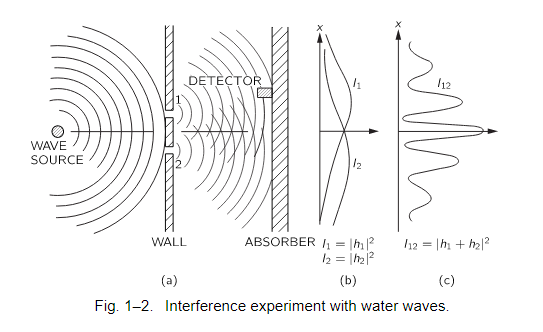
\includegraphics[scale=0.8]{double-slit}
	\caption{From Feynman's lectures of Physics}
\end{figure}

We know that the amplitude/propagator $K = A_1 + A_2$ leads to interference. \\

The basic idea behind the path integral comes from considering what happens when there are many many many more slits. This suggests that the propagator should be the sum over all paths of some functional $A[\gamma]$ that is the amplitude associated with each path:
\begin{align}
K =\sum_\gamma A[\gamma]
\end{align}
where 
\begin{align}
\boxed{K(q_f,t_f, q_i,t_i) = \bra{q_f} e^{i\had (t_f - t_f)/\hbar} \ket{q_i}}
\end{align}
is the propagator. \\


When there are infinitely many holds of infinitesimal size, the particle can be anywhere (since there's essentially no more holes), so we have the picture
\begin{figure}[!htb]
	\centering
	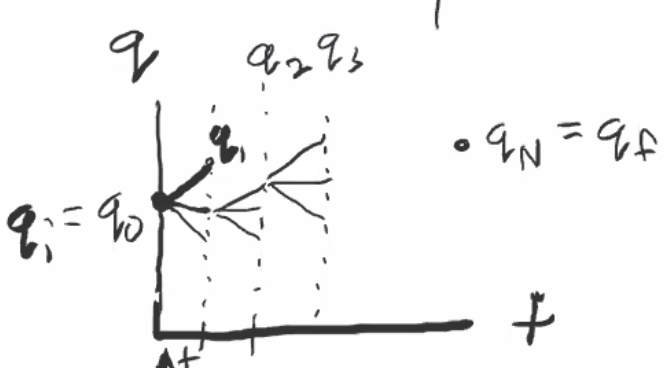
\includegraphics[scale=0.5]{time}
	\caption{From PI lecture by Dan Wohns}
\end{figure}
In this case, the sum over paths becomes an integral
\begin{align}
\sum_\gamma \to \lim_{N\to \infty}\int d q_1dq_2\dots dq_{N-1}
\end{align}


\subsection{Some properties}

\begin{prop}[Composition]
	Consider the path $\gamma_{12}$ composed of the path $\gamma_1$ followed by the path $\gamma_2$. Then
\begin{align}
A[\gamma_{12}] = A[\gamma_1] A[\gamma_2].
\end{align}
This implies (as we will see in the exercises) that
\begin{align}
K(q_f,t_f,q_i,t_i) = \int dy\,K(q_f, t_f,y,t_{int})K(y,t_{int},q_i,t_i).
\end{align}
\end{prop}


\begin{prop}[Classical Limit]
	When $\hbar \to 0$ and the action  $S \gg \hbar$, then the classical path becomes most important. 
\end{prop}


For most of the course, we will be consider actions that look like
\begin{align}
S = \int^{t_f}_{t_i} dt\, \f{1}{2}m\dot{p}^2(t) - V(q(t)).
\end{align}
The classical path satisfies the Euler-Lagrange equation: 
\begin{align}
\f{\delta S}{\delta q(t)} = 0.
\end{align}
This turns out to be 
\begin{align}
m\ddot{q} + V'(q) =0 
\end{align}
which is just Newton's second law of motion. \\


With these, we have 
\begin{align}
\int \mathfrak{D}q(t) e^{iS[q(t)]/\hbar}.
\end{align}
The composition property suggests that we should have an exponential, so that we can convert multiplication to summation. This says that all paths contribution with equal weight. So, the classical path is as important as the quantum path in the action. However, only paths such that $\delta S = 0$ contribute more to the propagator. \\

Consider the paths $q(t)$ and $q'(t) = q(t) + \eta (t)$ where $\eta(t)$ is some small perturbation, then 
\begin{align}
S[q'(t)] = S[q(t)] + \int dt\, \eta(t) \f{\delta S[q]}{\delta q(t)} + \mathcal{O}(\eta^2).
\end{align}

What happens in the general case is that 
\begin{align}
e^{iS[q]/\hbar} + e^{iS[q']/\hbar} \approx  e^{iS[q]/\hbar}\lp 1 + \exp\lb \f{i}{\hbar} \int dt\, \eta(t) \f{\delta S[t]}{\delta q(t)} \rb \rp
\end{align}
So, when $\hbar \to 0$, we get destructive interference. But if $\delta S/\delta q = 0$, we get constructive interference. So, even though all paths are equally important, it's also true that the classical path are ``more important'' than quantum paths, because they interference constructively. 








\newpage
\section{Propagator in real and imaginary time}


Last time, we guessed the form of the propagator. This time, we will derive in some detail the propagator in real and imaginary time. \\


What we're trying to compute is the propagator:
\begin{align}
K(q_f, t_f,q_i ,t_i) =  \int \prod_j^{N-1}   dq_j K (q_{j+1},t_{j+1}, q_j , t_j) \equiv  \int \prod_j^{N-1}   dq_j K_{q_{j+1},q_j}.
\end{align}
using the composition property that we discussed last time. Now this is starting to look like a path integral. \\

Now, we know that
\begin{align}
K_{q_{j+1},q_j} &= \bra{q_{j+1}}  e^{i\had \delta t/\hbar}  \ket{q_j}\nn\\
&\approx \braket{q_{j+1}}{q_j}   +  \bra{q_{j+1}}  \f{i\delta t \had}{\hbar} \ket{q_j} + \dots\nn\\
&= \delta(q_{j+1} - q_j) + \text{ Computed in Exercise } \nn\\
&= \int \f{dp_j}{2\pi \hbar} e^{ip_j(q_{j+1} - q_j)/\hbar} +  \text{ Computed in Exercises}
\end{align}

Putting everything together we get
\begin{align}
K_{q_{j+1},q_j} = \int \f{dp_j}{2\pi \hbar} e^{p_j(q_{j+1} - q_j)/\hbar}\lp 1 - \f{i\delta t \had}{\hbar} + \dots \rp
\end{align}
The term on the right hand side looks like a Taylor expansion for $e^{-i\delta \had t /\hbar}$. So, if we assume that $\had =  p_j^2 / 2m + V(q_j)$ then this integral becomes a Gaussian integral
\begin{align}
K_{q_{j+1},q_j} &= \int \f{dp_j}{2\pi \hbar} e^{i\delta t/\hbar (p_j\dot{q}_j  - p_j^2/2m - V(q_j) )  } \nn\\
&= \sqrt{\f{m}{2\pi i \delta t \hbar}} e^{(i\delta t /\hbar) ( mq_j^2/2 - V(q_j) )}.
\end{align}
Gaussian integrals are important in the study of path integrals, because they're among the integrals that we can evaluate exactly. \\

Staring at this for a bit, we notice that the exponential looks like part of the action. So, by multiplying together all these infinitesimal propagators, we get the entire action:
\begin{align}
K = \lp \f{m}{2\pi i \hbar \Delta t} \rp^{N/2} \int \prod^{N-1}_{j=1} dq_j \exp\lb \f{i \Delta t}{\hbar} \sum^{N-1}_{j=0} \lp \f{m\dot(q)_j^2}{2} - V(q_j) \rp \rb.
\end{align}
In the $N\to \infty$ limit, 
\begin{align}
K = \int \mathfrak{D}[q(t)] e^{iS(t)/\hbar}
\end{align}



Now we want to make the connection to imaginary time and statistical physics. Recall that
\begin{align}
K = \int \mathfrak{D}q(t) \exp\lb iS[q(t)]/\hbar \rb.
\end{align}
Now, the $i$ leads to oscillations in the integrand, which leads to questions about convergence of the integral. So, it would be much more convenient if $i$ wasn't there. This means we want to consider \textbf{imaginary time}. Why do we want to do this? Mathematically, it's generally easier. More important, if we make the exponential real, we can make connections to statistical physics. So we shall see a connection between quantum mechanics in imaginary time and statistical physics. Thirdly, in quantum mechanics we're interested in the ground states energy of Hamiltonians. Sometimes, it is possible to compute ground state energies using quantum mechanics in imaginary time. \\


To this end, consider $T = -i T_E$ where $E$ stands for Euclidean. Once we do that, we can computer the Euclidean propagator:
\begin{align}
K_E = \bra{q_f}  e^{-T_E \had /\hbar} \ket{q_i}
\end{align}
with $t \to -i \tau$. If we do that, then 
\begin{align}
iS[q(t)] = i\int^T_0 dt \lp \f{m}{2}\dot(q)^2  - V(q)\rp \mapsto -\int^{T_E}_0 d\tau \lp \f{m}{2}\dot(q)^2 + V(q) \rp
\end{align}
where the time derivative becomes derivative over $\tau$, so the relative sign between the kinetic and potential energy changes. With this, we have the Euclidean action:
\begin{align}
iS[q(t)] = -S_E[q(\tau)].
\end{align}
After this replacement, we can compute the Euclidean propagator:
\begin{align}
K_E = \int \mathfrak{D}[q(t)] e^{-S_E[q(\tau)] /\hbar}.
\end{align}

With this we can compare this to the expression for the partition function:
\begin{align}
\mathcal{Z}[\beta] = \sum_j e^{-\beta E_j}
\end{align}
by identifying $\beta = T_E/\hbar = 1/k_BT$ where now $T$ is temperature. It turns out that (which we will verify in the exercises)
\begin{align}
\mathcal{Z} = \int dq K_E(q,0,q,\beta\hbar).
\end{align}
Note that the ground state energy $E_0$ can be found this way:
\begin{align}
E_0 = \lim_{\beta \to \infty} \f{1}{\beta} \log \mathcal{Z}.
\end{align}
We can relate the propagator to the ground state energy, which is an observable of interest. \\



\subsection{Free Path Integrals}

Free path integrals are some of the path integrals we can compute exactly. These come from quadratic action $S$ in the variable $q$. For example,
\begin{align}
K_E = \bra{q_f}  e^{-\beta \had}  \ket{q_i}, \quad \had = p^2/2m.
\end{align}
This integral is easy (compared to oscillatory integrals) to compute, because the integral is just Gaussian. It turns out that
\begin{align}
K_E = \sqrt{\f{m}{2\pi \beta}} e^{-S[q_c]/\hbar} 
\end{align}
where $q_c$ is the classical trajectory. The way to derive this is via Gaussian integration techniques. \\


The key idea here is that in this case $K_E$ turns out to have the form with $N$-coupled Gaussian integrals. To understand this, we only need to understand a single integral. In any case, we can learn a lot of about path integrals by just looking at the case $N=1$. When $N=1$, we can actually can go through a lot of the details. When $N$ is larger, we don't gain much more knowledge. We will discuss, of course, what happens when $N \to \infty$. \\


Next, we will look at perturbation theory, where the action is no longer quadratic. Again, we will look at the case where $N=1$. We will also see where the path integral and perturbation theory fails. We will, of course, look at how we can address these failures. 




















\newpage

\section{Perturbation theory}


Consider the action
\begin{align}
S_E = \int d\tau \lb \f{1}{2}m\dot{q}^2(\tau) + \f{1}{2}m\omega^2q^2(\tau) + \f{\lambda}{4!}q^4(\tau) \rb
\end{align}
We want to compute the propagator:
\begin{align}
K_E = \int \mathfrak{D}[q(t)] e^{-S_E[q(\tau)]s/\hbar}
\end{align}
where we're working in Euclidean time. We want to compare this integral to 
\begin{align}
I = \int_\R dx e^{-f(x)/\hbar}.
\end{align}
The analogy we will keep in mind the following
\begin{align}
K_E \leftrightarrow I, \quad q(\tau) \leftrightarrow x, \quad S_E \leftrightarrow f.
\end{align}
Suppose that $f$ is some function with a global minimum at zero. If we want to find $I$, we want to find where $f(x)$ is minimum -- in this case it is near zero. Similarly, to approximate $K_E$, we want to find paths where the action $S[q]$ is smallest. This means we want places where $\delta S / \delta q = 0$. But of course this is just the equation of motion. This means we want to look at paths close the classical path $q_C$. \\

The strategy is to Taylor expand $f$, so that we can write the integral $I$ as
\begin{align}
I \approx \sum_{c_1,c_2,n}c_1 \int_\R dx x^n e^{-C_n x^2}
\end{align}
which we will show in the exercise. \\

The trick to evaluate these integrals is to add a source $J$:
\begin{align}
\int \mathfrak{D}[q(\tau)] \exp\lb -\f{1}{\hbar} \int d\tau \lp S[q] - J(\tau)q(\tau)\rp \rb.
\end{align}
The one-dimensional analog is 
\begin{align}
I = \int dx \,\exp\lb -x^2 + xJ \rb.
\end{align}
Note that
\begin{align}
\f{d}{dJ}I = \int dx\, x \exp\lb -x^2 + xJ \rb = \pi \f{J}{2}e^{J^2/4}\bigg\vert_{J=0} \implies \int dx\, x\exp(-x^2) = 0.
\end{align}
In general, this technique works when we evaluate path integrals. With this technique we can construct a systematic way to approximate path integrals. This systemic way is Feynman diagrams. 





\newpage

\section{Non-perturbative physics and quantum tunneling}
Recall that terms like $e^{-A/\lambda}$ are invisible to perturbation theory. In this section, we look at how we fix this problem in non-perturbative physics. In particular, we can look at phenomena like quantum tunneling. In this case, we are interested in the transmission coefficient:
\begin{align}
T \propto e^{-2/\hbar \sqrt{2m(V-E)}\,dx}
\end{align}
This is invisible to perturbation theory. Another example is meta-stable potential. Another example is a potential with two classically degenerate ground states. In this case, the transmission coefficient also has a similar form. \\

Recall the propagator amplitude:
\begin{align}
K_E = \int \mathfrak{D}[q(\tau)]  e^{-S_E[q(\tau)]/\hbar}
\end{align}
with 
\begin{align}
E_0 = -\lim_{\beta \to 0}\f{1}{\beta}\log K_E(q_0 ,\be\hbar/2, q_0 -\beta\hbar/2)
\end{align}
where we have shifted the time, which doesn't change the expression, of course. \\

What we're interested in is the decay rate for the following metastable potential (with no ground state):
\begin{figure}[!htb]
	\centering
	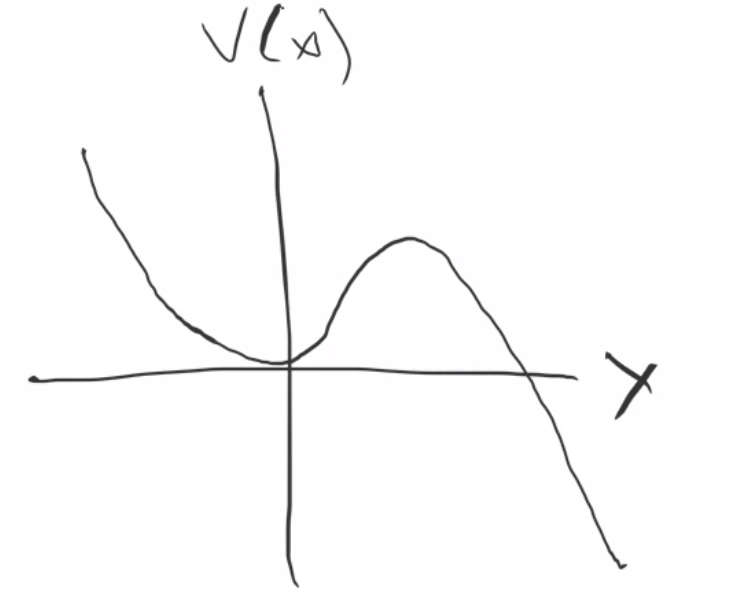
\includegraphics[scale=0.4]{metastable}
\end{figure}
While there's no notion of a ground state energy, we still have \textbf{resonant states} which are those with quantized complex energies. \\

The decay rate is given by
\begin{align}
\Gamma = 2\abs{\Im E_0}
\end{align}
which is why the decay rate is related to this setup. We want to compute $K_E$ using path integrals. To do this, we think about the example
\begin{align}
I = \int_\R e^{-f(x)/\hbar}\,dx.
\end{align}
Last time we looked at perturbation theory, which says that $f(x)$ has a global minimum at zero, then we get an expansion. Now, we can think about a slightly more general case where $f$ has several minima. Then expansions around all of the minima are roughly equally important. In this case, we have that 
\begin{align}
I &\approx \sum_{x_i} \int dx\, \exp\lb -\f{1}{\hbar}\lp f(x_i) + (1/2)f''(x_i) (x-x_i)^2 \rp \rb \times\lb 1+ \dots \rb \nn\\
&\approx \sum_{x_i}e^{-f(x_i)/\hbar}(1+ \mathcal{O}(\hbar^\al))\nn\\
&\approx \sum_{x_i}e^{-f(x_i)/\hbar}N[\bar{x}]\nn\\
\end{align}
as we have seen in the exercises. Now let's go back to the path integral. There might be multiple good trajectories, so we should sum over all of them:
\begin{align}
K_E = \sum_{\bar{q} = q_c} e^{-S_E[q(\tau)]/\hbar} N[\bar{q}] .
\end{align}
\begin{figure}[!htb]
	\centering
	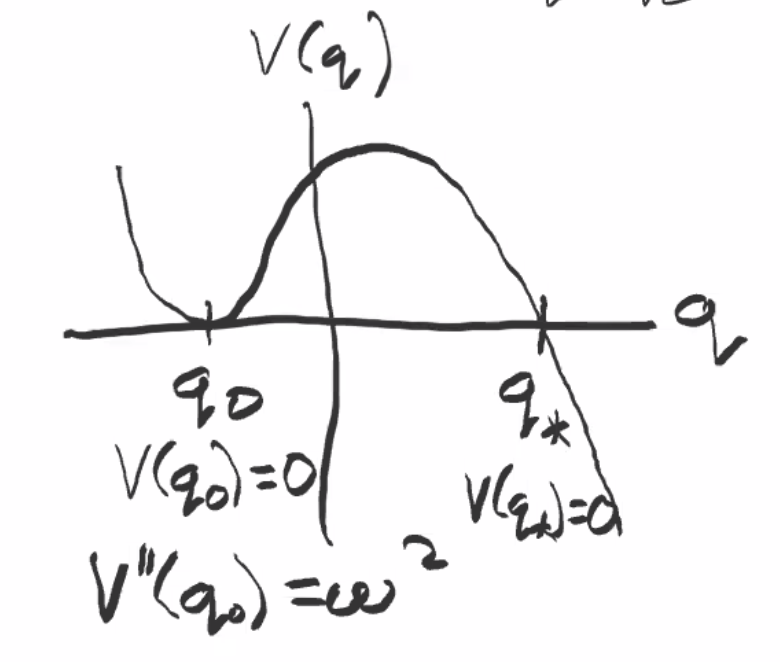
\includegraphics[scale=0.3]{meta}
\end{figure}
The decay rate is given by
\begin{align}
\f{\Gamma}{2} = \abs{\Im E_0}.
\end{align}
Then 
\begin{align}
E_0 = -\lim_{\beta \to 0}\f{1}{\beta}\log K_E(q_0 ,\be\hbar/2, q_0 -\beta\hbar/2)
\end{align}
The equation of motion is 
\begin{align}
-m d_\tau^2 \bar{q}(\tau) + V'(\bar{q}) = 0
\end{align}
with the boundary conditions $\bar{q}(\pm T_E/2) = q_0$ with $T_e = \beta\hbar$. We want to look at the limit where $\beta \to \infty$.\\

One other thing we care about is that the action should be finite. If the action is infinite than these trajectories don't contribute at all to the propagator.  

\newpage


\section{Topology and Particle Statistics}

Consider an amplitude 
\begin{align}
A = \sum_{\text{paths}} e^{iS[q_1(t),q_2(t)]}.
\end{align}
for two identical particles to go from $q_1, q_2$ at $t=0$ to some positions $q_1', q_2'$ at $t=T$. There are two possibilities of this happening: \textbf{direct} and \textbf{exchange} (since these are indistinguishable particles)
\begin{figure}[!htb]
	\centering
	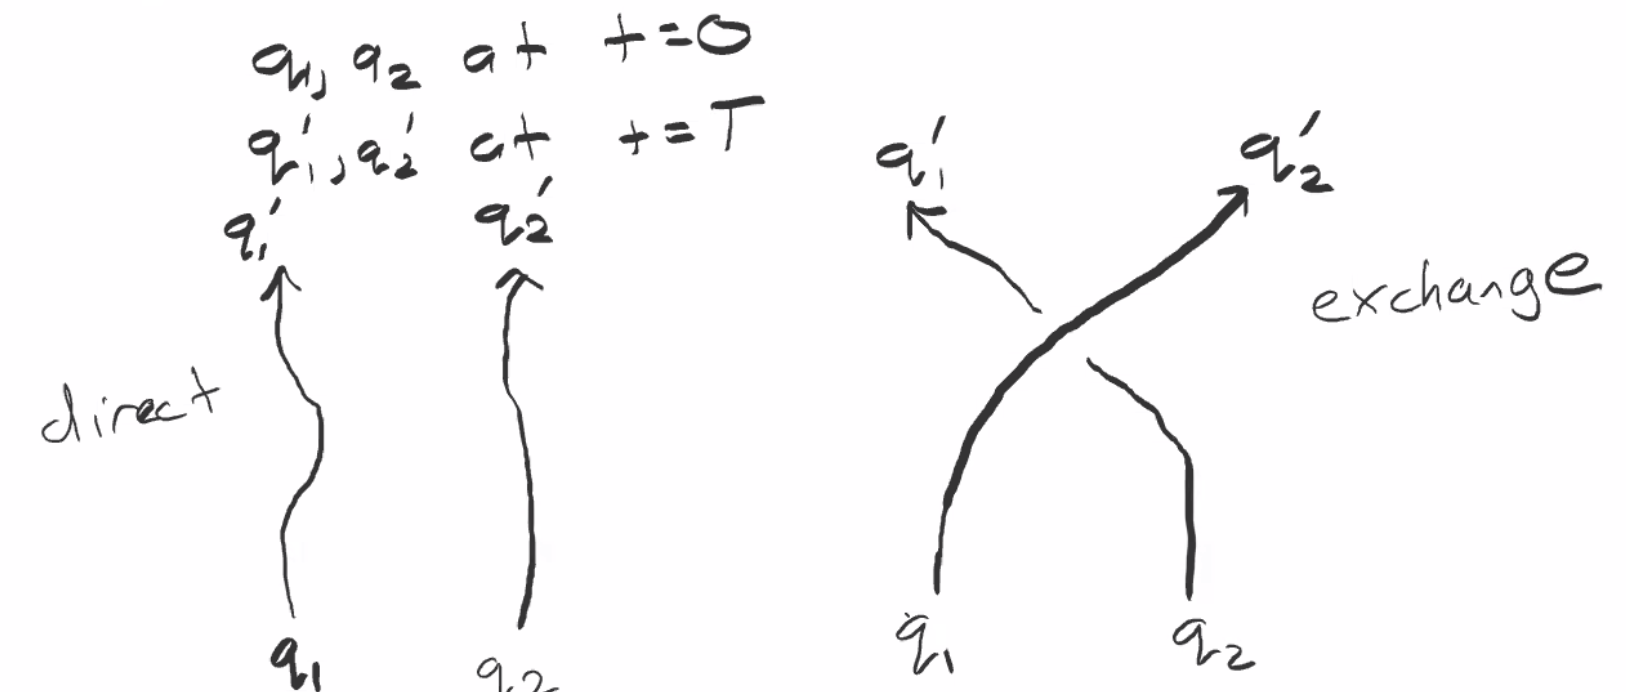
\includegraphics[scale=0.2]{paths}
\end{figure}
Note we assume things happening in three dimensions of space. \\ 

Now, what do the path integrals look like in both scenarios? Before we do this, let us introduce \textit{relative coordinates}:
\begin{align}
q(t) = q_2(t) - q_1(t)
\end{align}
and assume that $q(T) = q(0)$ for the direct path case and $q(T) = -q(0)$ for the exchange case. 
\begin{figure}[!htb]
	\centering
	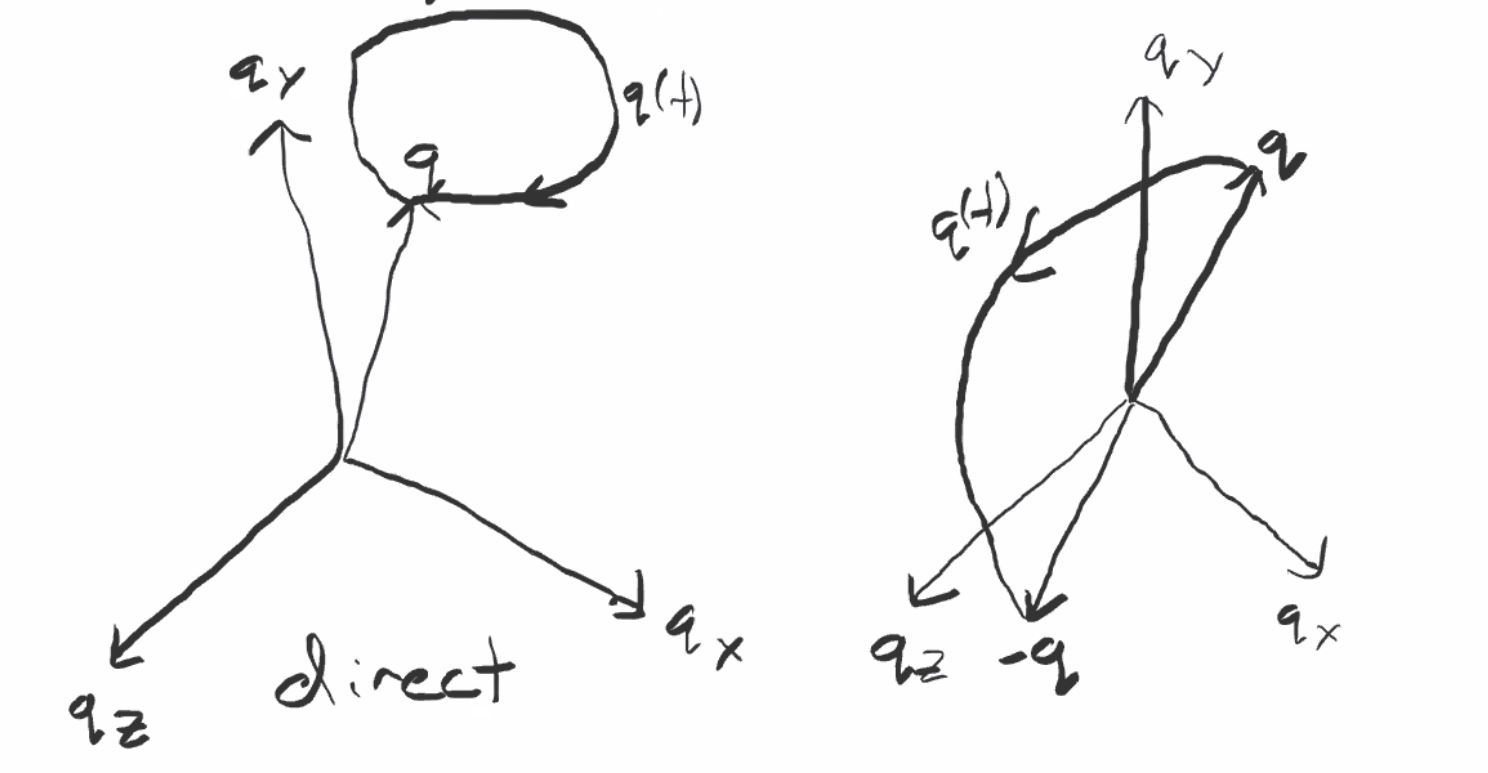
\includegraphics[scale=0.2]{paths1}
\end{figure}
This space of $q(\cdot)$ is called the \textbf{covering space}. The covering space is basically the three-dimensional Euclidean space. We also assume that particles cannot be at the exact same position at any given time due to some repulsion, so the covering space looks like $\R^3\setminus\{ 0\}$. The \textbf{configuration space} is half of the covering space: $(\R^3\setminus\{ 0\})\setminus \Z_2$, in which we make the identification $q \leftarrow -q$. \\

With this, the amplitude in the configuration space $A(q,T,q,0)$ is 
\begin{align}
A(q,T,q,0) &= \sum_{\text{direct}} e^{iS[q_1,q_2]} + \sum_{\text{exchange}} e^{iS[q_1,q_2]} \nn\\
&= \bar{A}(q,T,q,0) + \bar{A}(-q,T,q,0)
\end{align} 
where $q$ is the relative position and $\bar{A}$ are the amplitudes in the covering space. \\

We can also write, for $q'\neq q$,
\begin{align}
A^{\phi}(q',T,q,0) = \bar{A}(q',T,q,0) + e^{i\phi}\bar{A}(q',T,q,0). 
\end{align}
These amplitudes are well-defined in the covering space. The phase can be there because the SE is linear. We can also write
\begin{align}
A^{\phi}(q',T,q,0) = e^{i\al}A^\phi(-q',T,q,0) 
\end{align}
where the overall phase $\al$ and the exchange $q' \leftrightarrow q$ does not change the physics. In the covering space, this becomes
\begin{align}
\bar{A}(q',T,q,0) + e^{i\phi}\bar{A}(-q',T,q,0) = e^{i\al}\lp \bar{A}(-q',T,q,0) + e^{i\phi}\bar{A}(q',T,q,0) \rp
\end{align}
so we get that
\begin{align}
1 = e^{i(\al + \phi)}, \quad e^{i\phi} = e^{i\al}.
\end{align}
This means that $\phi = \al + 2\pi k$ and thus $\phi = \{ 0,\pi \} + 2\pi k$ . When $\phi = 0$, we get Bose-Einstein statistics (phase +1), and if $\phi = \pi$ then we get Fermi-Dirac statistics (phase -1).  




\newpage



\section{Applications}

\begin{itemize}
	\item Bohm-Aharonov effect.
	\item Path integrals not only compute propagators but also also anything other thing that can be computed in the other formulations of quantum mechanics. 
	\item Using path integrals where the variables are fermionic, i.e., integration variables are grassmann variables. Grassmann variables and grassmann integration is an entirely different field of study.
	\item Generalizing path integrals over the history of a particle to over the history of a field. This is one way to combine special relativity with quantum mechanics. This is one way to understand quantum field theory. 
	\item 
\end{itemize}





\newpage




\section{Exercises}



\noindent \textbf{1. Composition.} 
\begin{enumerate}
	\item In lecture we argued that the propagator $K$ can be written as a sum (or an integral) over paths $\gamma$ of a functional $A[\gamma]$. 
	\begin{align}
	K = \sum_\gamma A[\gamma].
	\end{align}
	Show that the propagator obeys the composition property
	\begin{align}
	K(q_f, t_f, q_i, t_i) = \int dy\, K(q_f,t_f,y,t_{int})K(y,t_{int},q_i ,t_i)
	\end{align}
	of $A$ has the factorization property
	\begin{align}
	A[\gamma_{12}] = A[\gamma_1]A[\gamma_2].
	\end{align}
	
	
	
	\begin{proof}
		Let $A$ satisfy the factorization property. Then, 
		\begin{align}
		K = \sum_{\gamma_1,\gamma_2}A[\gamma_1]A[\gamma_2] = \int \,dy \,\sum_{\gamma_1} A[\gamma_1] \sum_{\gamma_2} A[\gamma_2]
		\end{align}
		where the path $\gamma_1$ ends at $y$ and $\gamma_2$ starts at $y$. With this, it's straightforward:
		\begin{align}
		K &= \int \,dy \bra{q_f}e^{-i\had (t_f - t_{int})/\hbar}\ket{y}\bra{y} e^{-i \had (t_{int} - t_i)/\hbar} \ket{q_i}\nn\\
		&= \bra{q_f}e^{-i\had(t_f - t_{int} + t_{int} - t_i)/\hbar}\ket{q_i}   \nn\\
		&= K(q_f,t_f,q_i,t_i).
		\end{align}
		So, we're done, because from the first line we conclude
		\begin{align}
		K(q_f, t_f, q_i, t_i) = \int dy\, K(q_f,t_f,y,t_{int})K(y,t_{int},q_i ,t_i).
		\end{align}
	\end{proof}
	
	
	
	
	\item Explain why the factorization property
	\begin{align}
	A[\gamma_{12}] = A[\gamma_1]A[\gamma_2]
	\end{align}
	holds if $A[\gamma] = e^{iS[\gamma]/\hbar}$ where $S[\gamma]$ is the classical action of the trajectory $\gamma$.
	
	\begin{proof}
		We note that $S[\gamma_{12}] = S[\gamma_1] + S[\gamma_2]$ if $\gamma_{12}$ is composed of  $\gamma_1,\gamma_2$. So this factorization property follows.
	\end{proof}
	
	
	
	\item Suppose $A[\gamma] = C_1 e^{C_2 S[\gamma]}$ for some constants $C_1,C_2$. Which values of $C_1,C_2$ give rise to a composition property? 
	
	\begin{proof}
		$C_1$ must be constantly 1, so that the composition property is satisfied. $C_2$ can be any real or complex number. 
	\end{proof}
	

\end{enumerate}




\noindent \textbf{2. Classical Limit}
\begin{enumerate}
	\item Suppose $f(x)$ is a real function. Which values of $x$ provide the most important contribution to 
	\begin{itemize}
		\item $\int e^{-f(x)}\,dx$? Why? (Optional: what conditions should be placed on $f(x)$?)
		
		
		\begin{proof}
			The most important contribution to this integral is when $f$ is small, so $x$'s where $f(x)$ is small. 
		\end{proof}
	
	
		\item $\int e^{if(x)}\,dx$? Why? (Optional: what conditions should be placed on $f(x)$?)
		
		
		\begin{proof}
			The most important contribution to this integral is when $f$ changes slowly, so most comes from $x$ where $f'(x)$ small. 
		\end{proof}
	\end{itemize}



	\item The classical equation of motion for a particle with classical action $S$ is that the first-order variation vanishes:
	\begin{align}
	\delta S = 0.
	\end{align}
	A trajectory with $\delta S = 0$ is a classical trajectory. No extra conditions on the second-order variation of the action is required. Why does $A[\gamma] = e^{iS[\gamma]/\hbar}$ give the correct classical limit? 
	
	\begin{proof}
		Recall that $\delta S = 0$. So this sort of shows why $A[\gamma] = e^{iS[\gamma]/\hbar}$ works. We won't worry too much about the details here.
		
	\end{proof}
	
	\item What other choices $A[\gamma]$ give rise to the correct classical limit? Do they have a composition property? 
	
	\item Do any of the other possibilities you identified in 1(c) have the correct classical limit? 
\end{enumerate}





\noindent \textbf{3. First-Order Term.} By inserting the resolution of identity
\begin{align}
\bm{1} = \int\f{dp}{2\pi \hbar} \ket{p}\bra{p}
\end{align}
and using
\begin{align}
\braket{q}{p} = e^{ipq/\hbar}
\end{align}
show that the first-order term can be expressed as
\begin{align}
-i\f{\Delta t}{\hbar} \bra{q_{j+1}} \had\ket{q_j} = -i \f{\Delta t}{ \hbar} \int \f{dp_j}{2\pi \hbar} e^{ip_j(q_{j+1} - q_j)/\hbar} \lp \f{p_j^2}{2m} + V(q_j) \rp.
\end{align}
What changes at second order?


\begin{proof}
	This looks hard, but isn't hard at all. I won't show the full solution here, but I'll just sketch things out here. By inserting the resolution of identity we get
	\begin{align}
	&\,\,\,\bra{q_{j+1}} \int \f{d_i}{2\pi \hbar} \lp \f{p_i^2}{2m} + V(q_i) \ket{p_i} \bra{p_i} \rp \ket{q_j} \nn\\
	&= \int\f{dp_i}{2\pi \hbar} e^{ip_j(q_{j+1} - q_j)/\hbar}\lp \f{p_i^2}{2m} + V(q_i) \rp.
	\end{align}
	With this we're essentially done. 
\end{proof}




\noindent \textbf{4. Statistical Physics and Imaginary Time.} Show that the partition function 
\begin{align}
\mathcal{Z}[\beta] = \sum_j e^{-\beta E_j}
\end{align}
can be expressed as a sum over imaginary time propagators
\begin{align}
\mathcal{Z}[\beta] = \int dq\, K_E (q,\beta \hbar, q,0).
\end{align}


\begin{proof}
	Again, the resolution of identity is helpful here. Consider the energy eigenbasis, then we have
	\begin{align}
	\bm{1} = \sum_j  \ket{e_i}\bra{e_i}.
	\end{align}
	With this, and by identifying $-T_E\had/\hbar \equiv \beta\had$ we have
	\begin{align}
	\int dq K_E(q,0,q,\beta\had) &= \int dq \bra{q} e^{\beta \had} \ket{q} \nn\\
	&= \sum_i \int dq \bra{q}\ket{e_i} e^{\beta \had} \ket{q}\bra{e_i} \nn\\
	&= \int dq \sum_i \braket{e_i}{q} \bra{q}e^{-\beta\had}\ket{e_i}\nn\\
	&= \sum_i \bra{e_i} e^{-\beta \had} \ket{e_i}\nn\\
	&= \tr\lp e^{-\beta\had} \rp\nn\\
	&= \sum_n e^{-\beta E_i}.
	\end{align}
	where we have used the completion relation in the position space: 
	$$\int dq \ket{q}\bra{q} = \bm{1}.$$
	Of course, we can also go the other way from $\mathcal{Z}$ and use the completion relation in the energy eigenbasis. Either way, the solutions are equivalent.  
\end{proof}




\noindent \textbf{5. Path Integral Derivation of the Propagator.} In the path integral formalism the propagator in imaginary time is 
\begin{align}
K_E(q,\beta \hbar, q,0) = \lim_{N\to \infty} \lp \f{m}{2\pi \Delta \tau \hbar} \rp^{N/2}\int dq_1\dots dq_{N-1}\exp\lb -\tau \hbar \sum^N_{j=1} \f{m}{2} \lp \f{q_j - q_{j-1}}{\Delta \tau \hbar} \rp^2 \rb
\end{align}

\begin{enumerate}
	\item Show that the propagator can be rewritten as
	\begin{align}
	K_E(q,\beta\hbar, q,0) = &\lim_{N\to \infty} \lp \f{m}{2\pi \Delta \tau \hbar} \rp^{N/2} \lp \f{2\Delta \tau \hbar}{m } \rp^{\f{N-1}{2}}\nn\\&\times  
	\int dy_1\dots dy_{N-1}\exp\lb -\sum^N_{j=1}(y_j - y_{j-1})^2 \rb
	\end{align}
	
	\begin{proof}
		This is just change of variables, so I won't do that here. 
	\end{proof}
	
	
	\item Use induction to show that 
	\begin{align}
	\int dy_1,\dots dy_{N-1}\exp\lb -\sum^N_{j=1}(y_j - y_{j-1})^2 \rb = \lp \f{\pi^{N-1}}{N} \rp^{1/2} e^{-(y_N - y_0)^2/N}.
	\end{align}
	
	\begin{proof}
		Just use induction and crank. At one point we will have to evaluate a 1-dimensional Gaussian integral, but this shouldn't be a challenge. This one-dimensional Gaussian integral will introduce some factor $\pi^\al$ with other constants such that we get to the right hand side at iteration $N-1+1 = N$. In any case, this problem also looks hard but is quite easy. 
	\end{proof}
	
	
	\item Take the continuum limit $N\to \infty$ to recover the result from lecture:
	\begin{align}
	K_E(q,\beta \hbar, q,0) = \sqrt{\f{m}{2\pi \beta }} \exp\lb -\f{m(q_f - q_i)^2}{2\beta} \rb.
	\end{align}
	\begin{proof}
		Combining things in the previous parts, we get that in the $N\to \infty$ limit, we have
		\begin{align}
		K_E &= \lim_{N\to \infty}  \lp \f{m}{2\pi \Delta \tau \hbar} \rp^{N/2} \lp \f{2\Delta \tau \hbar}{m } \rp^{\f{N-1}{2}}\lp \f{\pi^{N-1}}{N} \rp^{1/2} e^{-(y_N - y_0)^2/N}\nn\\
		&= \dots
		\end{align}
		
		
		hmmm... There might be something wrong here... or might not. In any case, this is just a case of taking the limit correctly and using some change of variables. I won't go into the details.
	\end{proof}
	
\end{enumerate}








\noindent \textbf{6. Semi-Classical Limit.} 

\begin{enumerate}
	\item Let $f(x)$ be a real valued function. By expanding $f(x)$ around its minimal values $x_c$ show that we can approximate
	\begin{align}
	I = \int_\R dx\,e^{-f(x)/\hbar}
	\end{align}
	by
	\begin{align}
	I \approx \sum_{x_c}\sqrt{\f{2\pi \hbar}{f''(x_c)}}e^{-f(x_c)/\hbar}(1+ \mathcal{O}(\hbar^a))
	\end{align}
	\begin{proof}
		First, we Taylor expand $f(x)$ around $x_c$. Since $x_c$ is the minimum $f'(x_c)$ vanishes. After this, we can write the integrand as
		\begin{align}
		e^{a+bx^2+ cx^3} = e^{a+bx^2}\lp 1 + cx^3 + \dots \rp.
		\end{align}		
		With this, we can write out the approximation as in the problem.  With these, we have
		\begin{align}
		I &\approx \sum_{x_c}\int_\R e^{-f(x_c)/\hbar} e^{\f{-f''(x_c)(x-x_c)^2}{2\hbar}}\lp 1+ \f{f'''(x_c)(x-x_c)^3}{6\hbar} + \dots \rp \nn\\
		&\quad \times \lp 1 + \f{f^{(4)} (x_c)(x-x_c)^4}{24\hbar}+\dots \rp \,dx\nn\\
		&= \sum_{x_c}\sqrt{\f{2\pi \hbar}{f''(x_c)}}e^{-f(x_c)/\hbar}\lp 1 +   \mathcal{O}(\hbar^a)\rp.
		\end{align}
		
	\end{proof}


	
	\item Express the most important corrections to equation (2) in the form
	\begin{align}
	\int_\R dx\, C_1x^ne^{-C_2 x^2}
	\end{align}
	where $C_1,C_2$ are constants.
	\begin{proof}
		Note that when $n$ is odd, the corrections vanish. So, we only pay attention to the even $n$, the smallest of which is $n=4$. So the largest correction is 
		\begin{align}
		\int_\R \f{f^{(4)}(x_c)(x-x_c)^4}{24\hbar} e^{\f{-f''(x_c)(x-x_c)^2}{2\hbar}}\,dx.
		\end{align}
	\end{proof}
	
	
	\item Determine the value of $a$ in equation (2) by making a change of variables.
	\begin{proof}
		Now, making the substitution $y = (x- x_c)/\sqrt{\hbar}$. with this, we get $a=1$. Without loss of generality, let us set $x_c = 0$. This makes things a bit easier. Then $dx = \sqrt{\hbar}dy$ and the correction integral becomes
		\begin{align}
		\int_\R dy \sqrt{h}\hbar^2 \f{C_1}{\hbar} e^{-C_2 y^2} \sim \mathcal{\mathcal{O}(\hbar^{3/2})}.
		\end{align}
		Now because we have a leading factor of $\sim \sqrt{h}$ for the overall integral, the correction as written in the problem follows $\mathcal{O}(\hbar^1)$.
	\end{proof}
\end{enumerate}






\noindent \textbf{7. Perturbation Theory.}  In this problem we will show where perturbation theory breaks down.	
\begin{enumerate}
	\item Show that
	\begin{align}
	\exp\lb -\lambda\lp \f{d}{dJ} \rp^4 \rb\int_\R \exp\lb -x^2 + xJ \rb = \int_\R dx\,\exp\lb -x^2 - \lambda x^4 + xJ \rb.
	\end{align}
	Path integrals with interactions can be computed by taking derivatives of free path integrals with a source $J$ using generalizations of this formula. 
	\begin{proof}
			This is actually not hard. One questionable step we have to make is the interchanging of the sum and the integral. However, if we assume that the integral of a sum is equal to the sum of integrals then we can Taylor expand the leading factor in monomials of the operator $d/dJ$ and let it act on the integrand. Once this is done, we can rewrite the sum in the integrand as $e^{-\lambda x^4}$, as we should be able to do. I won't write out the math here, because it's already been done in my \href{https://huanqbui.com/LaTeX 20projects/HuanBui_QM/HuanBui_QM.pdf}{\underline{Q-CFT notes}}. 
	\end{proof}
	
	
	\item Use induction to show that
	\begin{align}
	\int_\R dx\, x^{2n}\exp\lb -\f{1}{2}ax^2 \rb = \lp \f{2\pi}{a} \rp^{1/2}\f{1}{a^n}(2n-1)!!
	\end{align}
	where $(2n-1)!! = (2n-1)(2n-3)\dots 5\cdot 3\cdot 1$. Hint: differentiate with respect to $a$. 
	\begin{proof}
		This boils down to doing induction correctly. This requires evaluating a quite simple Gaussian integral. Most of this will be algebra, so I won't write a solution here.
	\end{proof}


	\item Show that 
	\begin{align}
	\int_\R dx\,\exp\lb -x^2 - \lambda x^4 \rb = \sqrt{\pi}\sum^\infty_{j=0}\f{(-\lambda)^j (4j-1)!!}{2^{2j}j!}
	\end{align}
	\begin{proof}
		The key is to expand the factor $e^{-\lambda x^4}$ into a power series. This power series will contain powers of $x$:
		\begin{align}
		\int_\R dx\,\exp\lb -x^2 - \lambda x^4 \rb &= \sum_{j=0}^\infty \int_\R \f{(-\lambda)^j x^{4j}}{j!}e^{-x^2}\nn\\
		&= \sqrt{\pi}\sum^\infty_{j=0}\f{(-\lambda)^j (2\times 2j - 1)!!}{2^{2j}j!}\nn\\
		&= \sqrt{\pi}\sum^\infty_{j=0}\f{(-\lambda)^j (4j-1)!!}{2^{2j}j!}
		\end{align}
	\end{proof}
	
	
	
	\item Show that the series in part (c) diverges.
	\begin{proof}
		The series diverges because of the factorial terms -- they don't die out quickly enough, or not at all! 
	\end{proof}
	
	
	\item Which step in the derivation was not justified?
	\begin{proof}
		The problem is occurs when we swap the integral and the sum. It's not always a valid operation. So why do we still do this? We still do this because most problems can be solved this way. The series diverges sometimes, but the operation can give very good predictions. The series, while diverges, is asymptotic to the series
		\begin{align}
		\lim_{\lambda \to 0+} \f{ I(\lambda) - \sum^N_{j=0}a_j \lambda^j}{\lambda^N} = 0.
		\end{align}
		This means that we should be careful when using perturbation theory. Also, this points out a problem with perturbation theory. There are effects that can't be accounted for by perturbation theory. There are effects such that
		\begin{align}
		\lim_{\lambda \to 0+} \f{e^{-1/\lambda}}{\lambda^N} = 0
		\end{align}
		that are invisible to perturbation theory. These are phenomena such as tunneling rates or energy splitings.
	\end{proof}
	
\end{enumerate}





\noindent \textbf{8. Instantons} 
\begin{enumerate}
	\item We want to solve the equation 
	\begin{align}
	-\f{d^2\bar{q}}{d\tau^2}
	\end{align}
	with boundary conditions $\bar{q}(\pm T_E/2) = q_0$. These equations are the equations of motion of a particle with mass $m = 1$ moving in
	a potential. Make the analogy with a particle moving in a potential explicit, paying attention to the signs.
	
	\begin{proof}
		The EOM is the same as the EOM for a particle moving in an inverted potential. 
	\end{proof}
	
	
	\item There is a trivial solution to equations of motion and boundary conditions. What
	is it? What is the action of this trivial solution?
	
	\begin{proof}
		The trivial solution is that the particle stays at $q_0$ at all times. Non trivial solutions look like 
		\begin{figure}[!htb]
			\centering
			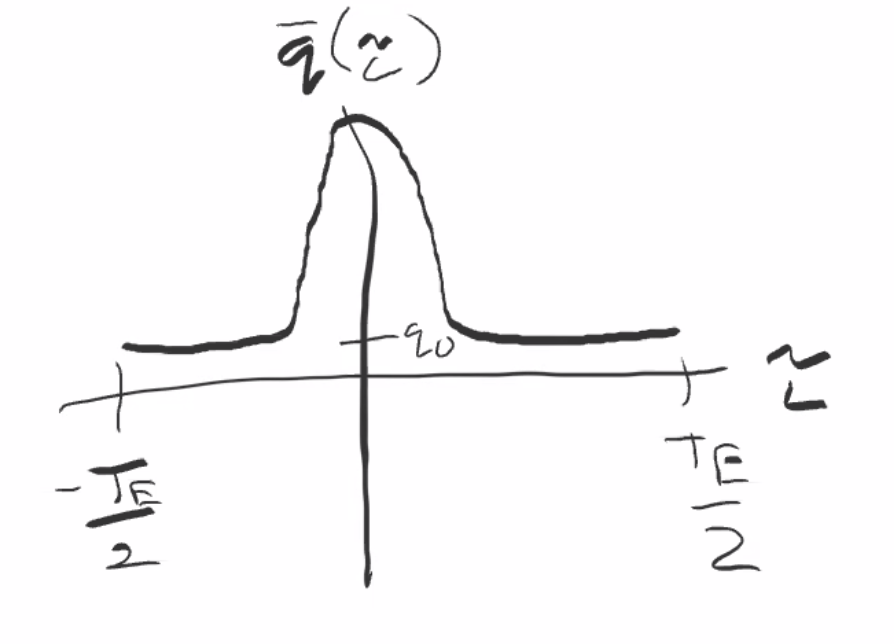
\includegraphics[scale=0.2]{bound}
		\end{figure}
	
	This solution has finite action:
	\begin{align}
	S_0 = S_E = \int d\tau \lp \f{1}{2}\lp \f{d\bar{q}}{d\tau} \rp^2 + V(\bar{q}) \rp
	\end{align}
	This is not the only solution, however. Another solution is where the particle bounces back and worth between $q_0, q_*$. The action in this case is just going to be $nS_0$ where $n$ is the number of times the particles bounces back and forth. In this case,
	\begin{align}
	K_E = \sum_{n=0}^\infty \f{T_E^n}{n!} e^{-n S_0/\hbar} = \exp\lb cT_E e^{-S_0/\hbar} \rb.
	\end{align}
	 
	
	\end{proof}
	
	

	
	\item Using conservation of energy, show that a solution to the equation of motion with
	zero energy has
	\begin{align}
	\bar{q}(\tau) -q_0 \approx e^{-\omega \abs{\tau}}
	\end{align}
	for large $\abs{\tau}$ (that is $\abs{\tau} \approx T_E/2$). 
	
	\begin{proof}
		Differentiate the differential equation, we will get $V'' = \omega^2$. Then integrate again. This is very hand-wavy, so it is understandable to be extremely confused.  
	\end{proof}
	
	
	
	
	\item We are interested in the $T_E \to \infty$ limit. Is the action of the solution you found finite
	and non-zero in this limit?
	
	\begin{proof}
		This is more or less straightforward. 
	\end{proof}
	
	
	\item Change integration variables and use conservation of energy to show that the action
	\begin{align}
	S_0 = \lim_{T_E\to \infty} \int^{T_E/2}_{-T_E/2} d\tau \lp \f{1}{2}\lp \f{d\bar{q}}{d\tau} \rp^2 + V(\bar{q}) \rp
	\end{align}
	of the solution you found can be expressed as
	\begin{align}
	S_0 = 2\int^{q_*}_{q_0}d\bar{q}\, \sqrt{2V(\bar{q})}
	\end{align}
	where $q_*$ is the other point where the potential vanishes $V (q_*) = 0$. 
	
	\begin{proof}
		
	\end{proof}
	
	\item Are there any solutions with non-zero energy with finite action in the $T_E \to \infty$ limit? 
	
	\begin{proof}
		
	\end{proof}
	
	\item Are there any other solutions with zero energy and finite action?
	
	\begin{proof}
		
	\end{proof}
\end{enumerate}





\noindent \textbf{9. Anyons.} 
$\,$
\begin{enumerate}
	\item In two spatial dimensions we can also write the amplitude for two particles with
	initial relative position $\bm{q}$ to propagate to the relative position $\bm{q}'$ in a time $T$ as 
	\begin{align}
	A(\bm{q}',T,\bm{q},0) = \sum_{\text{paths}} e^{iS[\bm{q}_1(t), \bm{q}_2(t)]}
	\end{align}
	As in lecture we will assume the particles cannot be at the same point due to some
	strong repulsive short range interaction. If the particles are identical, what is the
	configuration space? What is a natural covering space?
	
	
	\begin{proof}
		 $(\R^2\setminus\{0\})\setminus \Z_2$ and $\R^2\setminus \{0\}$. 
	\end{proof}
	
	
	
	\item As in three spatial dimensions the paths where the initial and final relative positions
	are the same $\bm{q} = \bm{q}'$ can be classified into topological classes. These paths can be
	characterized by the angular displacement $n \pi$ of the relative coordinate where $n$ is an integer. Sketch some of these paths. Argue that two paths with angular displacements $n\pi$ and $m\pi$ are topologically distinct if $m\neq n$.
	
	\begin{proof}
		Two paths are topologically equivalent if they can be smoothly deformed into another. We want to show that there are infinitely many classes of topologically distinct paths. Here are the pictures:
		\begin{figure}[!htb]
			\centering
			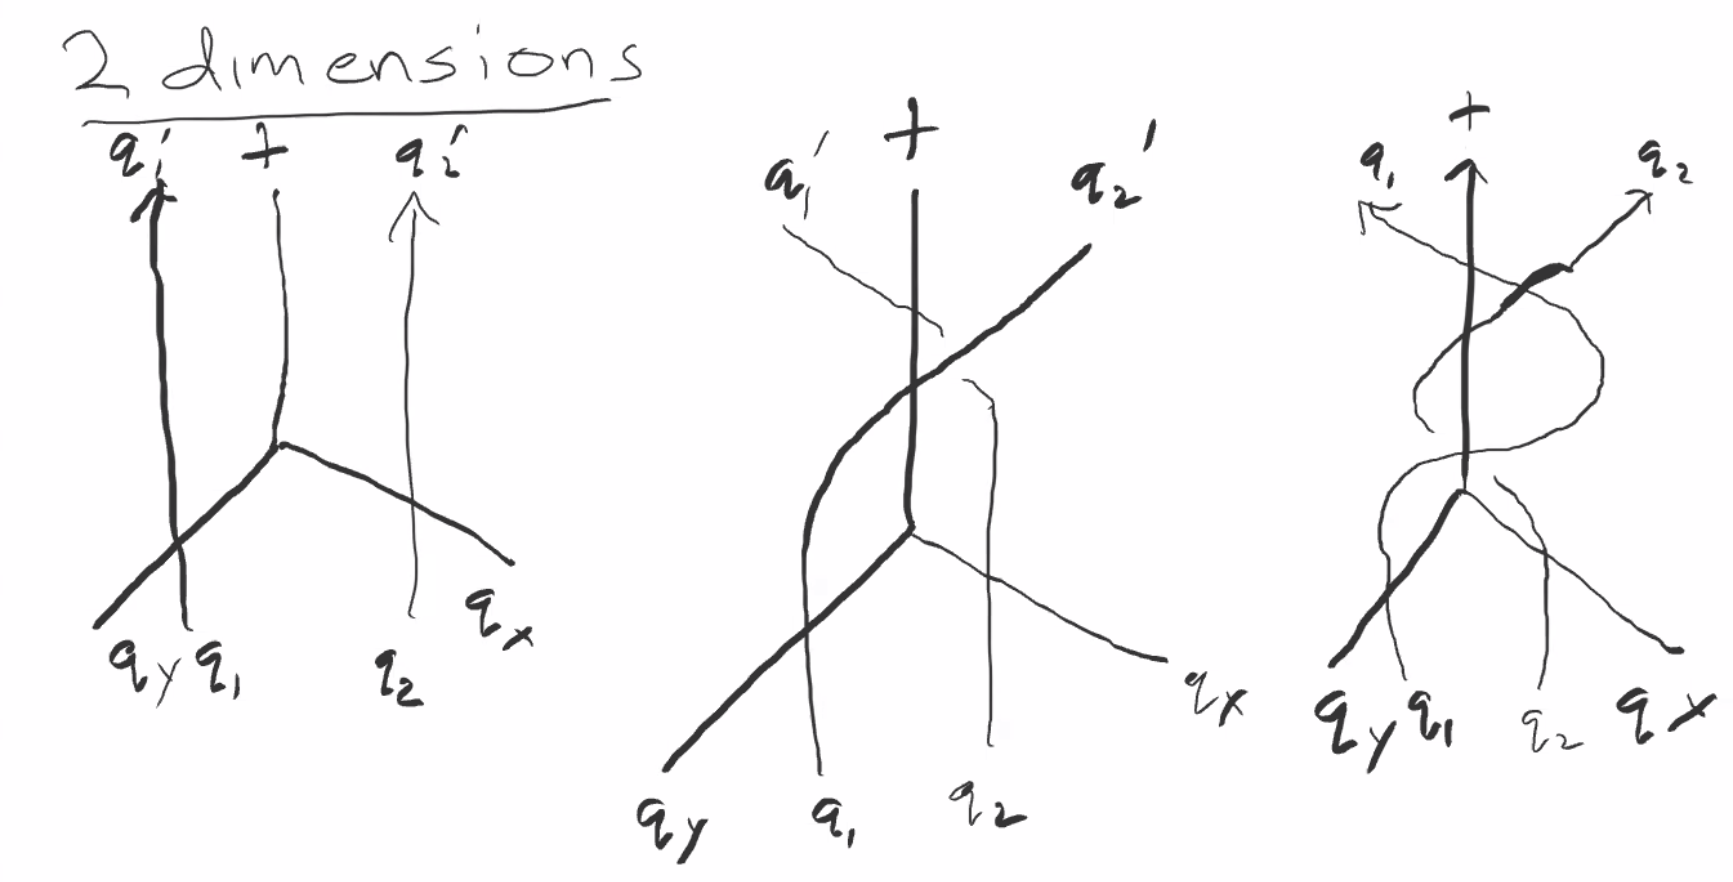
\includegraphics[scale=0.25]{paths3}
		\end{figure}
	There's no way to ``untangle'' the paths in two dimensions (which is something we can do in 3 dimensions), so these are topologically distinct paths. In the first case, the net angular displacement is 0. The subsequent ones are $\pi, 2\pi, \dots$. So, the $n$ here is the number of exchanges, which corresponds exactly its topological class.
	\end{proof}
	 
	
	
	\item Argue that in polar coordinates $\bm{q} = (q,\theta)$ the path integral in configuration space $A(\bm{q}, T, \bm q, 0) = A(q,\theta,T,q,\theta,0)$ satisfies
	\begin{align}
	A(q',\theta'+\pi , T, q,\theta,0) = e^{i\phi} A(q',\theta', T, q, \theta,0).
	\end{align}
	
	\begin{proof}
		From the exercise above, we get that $A$ is a sum over all topological classes $n: -\infty \to \infty$:
		\begin{align}
		A = \sum_{n=-\infty}^{\infty} C_n \bar{A}_n.
		\end{align} 
		Now, if we add $\pi$ to the final relative displacement, we get one more exchange. In the covering space, $n$ one bigger, but in the configuration space it is the same, so we get a phase. So we get
		\begin{align}
		A(\theta'+\pi) = e^{-i\phi} A(\theta').
		\end{align}
	\end{proof}
	
	
	
	\item The path integral in configuration space $A(\bm q, T , \bm q,0)$ can be written as a sum of path integrals in the covering space $\bar{A}_n(\bm q, T ,\bm q ,0)$
	\begin{align}
	A(\bm q, T, \bm q, 0) = \sum^{\infty}_{n=-\infty} \bar{A}_n (\bm q , T , \bm q,0)
	\end{align}
	where only paths with angular displacement $n\pi$ contribute to the path integral $\bar{A}_n(\bm q, T, \bm q, 0)$. If we add phases $C_n$ as in lecture, the amplitude in polar coordinates $\bm q = (q,\theta)$ becomes
	\begin{align}
	A(q,\theta, T,q,\theta,0) = \sum^{\infty}_{n=-\infty} C_n \bar{A}_n(q,\theta,T,q,\theta,0).
	\end{align}
	Use equation 
	\begin{align}
	A(q',\theta'+\pi , T, q,\theta,0) = e^{i\phi} A(q',\theta', T, q, \theta,0)
	\end{align}
	to show that
	\begin{align}
	C_n = e^{i\phi}C_{n-1}.
	\end{align}
	 
	
	\begin{proof}
		From the item above, we basically have a shifted sum. The index shift by 1 when we add $\pi$. So
		\begin{align}
		C_n = e^{i\phi}C_{n-1}.
		\end{align}
		
	\end{proof}



	\item Are there any constraints on the phase $\phi$? 
	
	\begin{proof}
		$\phi \in \R$, i.e., there are no constraints. This means we not only get BE and FD statistics but also fractional statistics such as anyons. They haven't been observed, but they are used to study other phenomena (e.g. fractional quantum Hall effect). 
	\end{proof}
\end{enumerate} 





\newpage









































\chapter{Symmetries}

\textbf{Instructor:} Giuseppe Sellaroli\\

The aim of this course is to  explore some of the many ways in which symmetries play a role in physics. We'll start with an overview of the concept of symmetries and their description in the language of  group theory. We will then discuss continuous symmetries and infinitesimal symmetries, their fundamental role in Noether's theorem, and their formalization in terms of Lie groups and Lie algebras. In the last part of the course we will focus on symmetries in quantum theory and introduce representations of (Lie) groups and Lie algebras.


\newpage


\section{Review: Equivalence Classes}


\subsection{Equivalence relations}


An equivalence relation is a special kind of binary relation. A
(homogeneous) binary relation on a set $X$ is a way of encoding a relationship between two elements of $X$. Given a relation $R$ we use the notation $xRy$ to mean ``$x$ is related to $y$.'' \\

Examples of relations are $=,<,>, \leq, \geq$ on $\mathbb{R}$. \\

\begin{defn}[Homogeneous binary relation]
	A homogeneous binary relation on a set $X$ is a set $R \subset X \times X$ of pairs of
	elements of $X$. When $(x,y) \in R$ we say that $x$ is relate to $y$, which we also indicate with the less cumbersome notation $xRy$.  
\end{defn}

We can now define equivalence relations.



\begin{defn}[Equivalence relation]
	An equivalence relation on a set $X$ is homogeneous binary relation $R$ that satisfies the following properties:
	\begin{itemize}
		\item Reflexive: $xRx \forall x\in X$.
		\item Symmetric: $xRy \implies yRx$.
		\item Transitive: $xRy, yRz \implies xRz$
	\end{itemize}
	These properties are chosen as they encode the fundamental features of the notion of
	things being ``equivalent.''
\end{defn}

Equivalence relations are often denoted by the symbol $\sim$. In this case we read $x\sim y$ as ``$x$ is equivalent to $y$.'' 





\subsection{Equivalence Classes}

Now that we know what an equivalence relation is, we can define the extremely useful concept of equivalence class.


\begin{defn}
	Let $\sim$ be an equivalence relation on $X$. The equivalance class of $x \in X$ is the set 
	\begin{align}
	[x]_\sim = \{ y\in X \vert y\sim x   \}
	\end{align}
	of all the elements in $X$ equivalent to $x$. We often drop the subscript and just write $[x]$ if there is no risk of confusion. Note that
	\begin{align}
	[x]_\sim = [y]_\sim, \quad \forall y \in [x]_\sim,
	\end{align}
	that is we can label the equivalence class using any of its elements. The element that we
	choose as the label is called the representative of the equivalence class.
\end{defn}



Equivalence classes are essentially buckets in which we put elements of X that are equivalent
to each other. Inequivalent elements end up in different equivalence classes. One way of
thinking about this is that an equivalence class is a way to encode as a single object the
properties common to its elements, which are otherwise indistinguishable.


\begin{exmp}
	An example of equivalence relation appears in modular arithmetic. Let's consider the simplest case of the integers modulo 2. We define an equivalence relation $\sim$ on $\mathbb{Z}$ by
	\begin{align}
	x\ sim y \implies x-y = 2k, k\in \mathbb{Z},
	\end{align}
	that is $x,y$ are equivalent if they differ by a multiple of two. If you want, you can check that this is indeed an equivalence relation as an exercise. There are only two distinct equivalence classes, which are the respectively the sets of even and odd integers. The sets of integers modulo 2 is
	defined as

	\begin{align}
	\mathbb{Z}_2 = \{ [0], [1]  \}.
	\end{align}
	Although this is a set of sets, we really want to pretend that it's a set of numbers. To do
	that, we define a way to add elements in $\mathbb{Z}_2$. The obvious choice is
	\begin{align}
	[a] + [b] = [a+b],
	\end{align}
	but at this stage this expression is purely formal: since we are specifying this operation
	through the sum of the representatives of each class, we need to make sure that the definition
	is actually independent of the choice of representatives (since they should be equivalent).
	This happens all the time when dealing with equivalence classes! In this case we are fine, because of the rules of adding odd and even numbers. 
\end{exmp}



\begin{exmp}
	Here’s an example from quantum physics. Let $\had$ be the Hilbert space of a quantum theory. While extremely useful, the states $\ket{\psi} \in \had$ are not \textit{physical}, where physical is meant as something that can be measured. The physical quantities in a quantum theory are the expectation values of the observables in a given state, that is 
	\begin{align}
	\langle A \rangle_\psi = \f{\bra{\psi}A\ket{\psi}}{\braket{\psi}}.
	\end{align}
	Now consider another state $\ket{\phi} = \lambda{\psi}$, with $\lambda \in \mathbb{C}\setminus \{0\}$. For any observable $A$ we have
	\begin{align}
	\langle A \rangle_\phi = \f{\abs{\lambda}^2}{\abs{\lambda}^2}\f{\bra{\psi}A\ket{\psi}}{\braket{\psi}} = \langle A \rangle_\psi.
	\end{align}
	This means that the states $\ket{\psi}$ and $\ket{\phi}$ are physically indistinguishable. It is then natural to consider them equivalent, and define the equivalence relation 
	\begin{align}
	\ket{\psi} \sim \ket{\phi} \iff \ket{\phi} = \lambda\ket{\psi}, \quad \lambda \in \mathbb{C}\setminus \{0\}.
	\end{align}
	
	The set 
	\begin{align}
	P(\had) = \{ [\ket{\psi}] \vert \ket{\psi} \in \had\setminus\{0   \}
	\end{align}
	is called th \textit{projective Hilbert space} associated to $\had$, and can be interpreted as the set of all distinguishable quantum states. The zero vector was removed as it does not describe any physical state (expectation values don't make sense for the zero vector). \\
	
	In a sense $P(\had)$ is the true set of states of a quantum theory. The reason why we work with $\had$ instead is that the latter is a vector space, which comes with a ot of nice properties and allows for an easy description of the superposition principle. 
	
	
	
\end{exmp}




\newpage



\section{Definition of symmetry}

We can't really give a mathematical definition of symmetry, because it depends on the context. But in any case we can define ``symmetry'' like this.

\begin{defn}[Symmetries]
	Loosely speaking, a symmetry is a transformation of $A$ that leaves $B$ invariant. 
\end{defn}

The idea is that $A$ and $B$ are not necessarily the same thing. 

\begin{exmp}
	If $B$ is the golden spiral and $A = \mathbb{R}^2$. When $A$ is scaled, $B$ remains invariant. 
\end{exmp} 

\begin{exmp}
	Consider a Lagrangian,
	\begin{align}
	S = \int d^4x\,\lag
	\end{align}
	and $B = S$  and $A$ is time, which we translate. We can see that $S$ is invariant under time translation. 
\end{exmp}


Some properties:
\begin{itemize}
	\item (Identity) ``Doing nothing'' is a symmetry. It is trivial, but is a symmetry nonetheless. This is also called the ``identity'' transformation.
	
	\item (Inverses) Symmetries are invertible. 
	
	\item (Composition) Compositions of symmetries are also symmetries. 
\end{itemize}



\section{Elements of group theory}


\begin{defn}
	A group is a set $G$ together with an operation $* : G\times G \to G$ satisfying the following properties:
	\begin{itemize}
		\item There is an identity element: $g*e = e*g = g, \forall g\in G$
		
		\item Each element of $G$ has an inverse, i.e., $\forall g\in G, \exists g^{-1}\in G$ s.t. $g^{-1}* g = g * g^{-1} = e \in G$.
		
		
		\item The operation $*$ is associative, that is  $a*(b*c) = (a*b)*c, \forall a,b,c\in G$.
	\end{itemize}

	Additionally, we say that the group $G$ is abelian/commutative if $a*b = b*a, \forall a,b\in G$. 
\end{defn}



\begin{defn}[Subgroups]
	Let $G$ be a group with operation $*$. A subgroup of  $G$ is a subset $H \subset G$ that contains the identity element and is closed under the operation $*$ and under inversion, that is 
	\begin{itemize}
		\item $e\in H$
		\item $a*b \in H \,\forall a,b\in H$
		\item $a\in H \implies a^{-1}\in H$.
	\end{itemize}
	The notation $H \leq G$ is commonly used to indicate that $H$ is a subgroup of $G$. 
\end{defn}


\begin{defn}[Group homomorphism]
	A group homomorphism is a map $\varphi: G \to H$ between two groups $G$ and $H$ such that 
	\begin{align}
	\varphi(a*_G b) = \varphi(a)*_H \varphi(b), \forall a,b \in G.
	\end{align}
\end{defn}





\begin{defn}[Kernel of a group homomorphism]
	The kernel of a group homomorphism $\varphi: G\to H$ is the set 
	\begin{align}
	\ker\varphi = \{ g\in G \vert \varphi(g) = e_H   \}
	\end{align}
	of all the elements of $G$ that are sent to the identity in $H$. 
\end{defn}

\begin{prop}
	A group homomorphism $\varphi: G\to H$ is injective if and only if the kernel is trivial: $\ker \varphi = \{ e_G\}$.
\end{prop}

\begin{proof}
	$\,$\\
	\begin{itemize}
	\item $(\rightarrow)$, if $\varphi$ is injective, then at most one thing can be sent to $e_H$. This means that $\ker\varphi = \{ e_G \}$.
	
	\item $(\leftarrow)$ Let $a,b\in G$ such that $\varphi(a) = \varphi(b) \implies e_H = \varphi(a)^{-1}\varphi(b) = \varphi(a^{-1})\varphi(b) = \varphi(a^{-1}b) $. But this means $a^{-1}b \in \ker{\varphi} \implies a^{-1}b = e_G \implies a=b$. So $\varphi$ is injective. 
	
	\end{itemize}
\end{proof}





\begin{defn}[Isomorphisms]
	Two groups $G$ and $H$ are isomorphic (denoted by by $G\sim H$) if there exists an invertible group homomorphism $\varphi: G \to H$. Such a map is called an isomorphism between $G$ and $H$. 
\end{defn}


\begin{defn}[Normal Subgroup]
	Let $G$ be a group. A subgroup $N\leq G$ is called \textit{normal} if 
	\begin{align}
	g n g^{-1} \in N, \forall g\in G, \forall n \in N.
	\end{align}
	The notation $N \trianglelefteq G$ is commonly used to indicated that $N$ is a normal subgroup of $G$. 
\end{defn}


\begin{defn}[Quotient Group]
	Let $N \trianglelefteq G$. We can define an equivalence relation on $G$ as
	\begin{align}
	g \sim h \iff h^{-1}g \in N
	\end{align} 
	with equivalence classes
	\begin{align}
	[g] = \{  h\in G \vert h^{-1}g \in N  \}.
	\end{align}
	The quotient group $G/N \equiv G \mod N$ is the set of equivalence classes
	\begin{align}
	G/N = \{ [g] \vert g\in G  \}
	\end{align}
	which is made into a group by defining
	\begin{align}
	[g][h] = [gh], \quad [g]^{-1} = [g^{-1}], \quad e_{G/N} = [e_G].
	\end{align}
\end{defn}


We note that the equivalence class does not require $N$ be normal. However, to turn the equivalence classes into a group, we require that $N$ is normal. 







\begin{thm}[First Isomorphism Theorem]
	Let $\varphi: G \to H$ be a group homomorphism. Then:
	\begin{itemize}
		\item $\Im \varphi$ is a subgroup of $H$.
		\item $\ker\varphi$ is a normal subgroup of $G$.
		\item $\Im \varphi$ is isomorphism to the quotient group $G / \ker\varphi$.
	\end{itemize}
\end{thm}


The notion that $\Im \varphi \sim G/\ker\varphi$ is important. This will appear again when we see Lie groups. 






\section{Examples: Symmetry \& Group Theory }

\begin{exmp}
	$(\mathbb{Z},+), (\mathbb{R},+), (\mathbb{C},+), \dots$ are abelian groups. 
\end{exmp}

\begin{exmp}
	$(\mathbb{R} \setminus \{0\}, \times)$ 
\end{exmp}

\begin{exmp}
	Invertible $n\times n$ matrices, $GL(n,\mathbb{R})$ under usual matrix multiplication. 
\end{exmp}

\begin{exmp}
	Circle group $S = \{(x,y) \in \mathbb{R}^2  \vert x^2 + y^2 = 1    \}$. Identity $(x,y) \in S$ with a complex number $z = x+iy$. Then use complex number multiplication. This works because $\abs{z} = 1 \implies z= e^{i\theta}$.
\end{exmp}




\begin{exmp}[Isomorphism]
	Consider the two groups $(\mathbb{R},+)$ and $(\mathbb{R}^+\setminus\{0\}, \times)$. The exponential map: $x\in R \mapsto e^x$. This map is obviously invertible. It is also a group homomorphism because it relates multiplication in the target group to addition in the reals. So, the two groups are isomorphic. \\
	
	This is particularly useful when we want to move from additive groups to multiplicative groups. \\
	
	This map is related to Lie groups, etc which we will see later.  
\end{exmp}









\newpage



\section{Continuous and discrete symmetries}

We will be quite vague with these definitions. 



\subsection{Discrete Symmetries}


Think of rotating polygons. Rotations that leave the polygon invariant are in integer steps. This is a prototype example of what a discrete symmetry is. 

\begin{figure}[!htb]
	\centering
	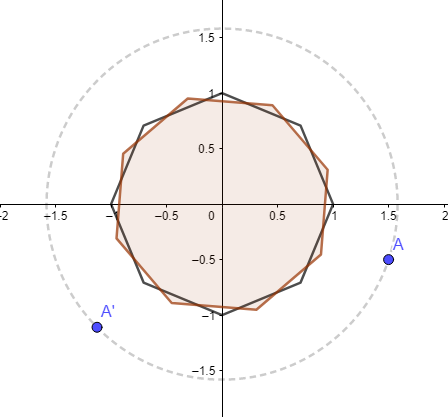
\includegraphics[scale=0.5]{polys}
\end{figure}

We can also easily define equivalence classes etc and see how the first isomorphism comes up, but we won't worry about that. \\

The idea of discrete symmetries is this: there is a discrete parameter for the group elements. 






\subsection{Continuous Symmetries}

In view of the previous example, we can consider rotating a circle. 
\begin{figure}[!htb]
	\centering
	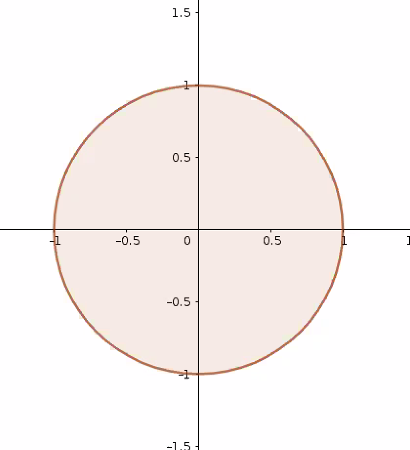
\includegraphics[scale=0.3]{circ}
\end{figure}


Obviously we can rotate by any angle and keep the circle invariant. \\


The idea of continuous symmetries is this: there is a continuous parameter for the group elements. Consider $\epsilon \in \mathbb{R}^+$ and take $\epsilon \mapsto \psi(\epsilon) = g_\epsilon \in G$. $\psi$ is a group homomorphism. Now, if there is a \textbf{topology} on $G$ such that $\psi$ is continuous, then we say $\{ g_\epsilon \vert \epsilon \in \mathbb{R}^+  \} = \Im(\psi)$ is continuous. This is quite vague, but is essentially the idea. \\


The group $\{ g_\epsilon \vert \epsilon \in \mathbb{R}^+   \}$ is called a \textbf{one-parameter subgroup}. One-parameter subgroups satisfy the following properties:
\begin{itemize}
	\item $g_0 = e_G$
	\item $g_{-\epsilon} = g_\epsilon^{-1}$
	\item $g_{\epsilon + \epsilon'} = g_\epsilon g_{\epsilon'}$. This means the the one-parameter subgroup is abelian.
\end{itemize}

For example consider $g_\theta$ define by $2\times 2$ rotation matrix $R_\theta$. We can check that $g_\theta$ satisfies all of the properties above.  


























\section{Infinitesimal symmetries}

Rotations are a particular example of infinitesimal symmetry. Just like calculus, we want to talk about ``derivatives.'' Assume that that $\epsilon \in \mathbb{R} \mapsto g_\epsilon \in G$ is a ``smooth'' map. Here, ``smooth'' means infinitely differentiable, or ``as nice as we want.'' This only makes sense if we have a ``differentiable structure'' on $G$. \\

Now, if the map above is smooth, we can linearize it. (Now we're doing things in the physicist's way). To linearize:
\begin{align}
g_\epsilon = g_0 + \epsilon \f{d}{d\epsilon}g_\epsilon\bigg\vert_{\epsilon = 0} + \mathcal{O}(\epsilon^2).
\end{align}
The infinitesimal symmetry is then 
\begin{align}
g_\epsilon = g_0 + \epsilon \f{d}{d\epsilon}g_\epsilon\bigg\vert_{\epsilon = 0}.
\end{align}
where $g_0$ is the identity.\\

More formally, infinitesimal symmetry has the form $e + \epsilon X$ where 
\begin{align}
X = \f{d}{d\epsilon}\bigg\vert_{\epsilon = 0} g_\epsilon.
\end{align}


\begin{exmp}
	Consider 
	\begin{align}
	R_\theta = \begin{bmatrix}
	\cos\theta & \sin\theta \\ -\sin\theta & \cos\theta
	\end{bmatrix}
	\end{align}
	With this,
	\begin{align}
	\f{d}{d\theta}\bigg\vert_{\theta = 0} R_\theta = \begin{bmatrix}
	0 & 1 \\ -1 & 0
	\end{bmatrix}
	\end{align}
	This means that the Taylor expansion of $R_\theta$ around 0 is given by
	\begin{align}
	R_\theta = \begin{bmatrix}
	1 & 0 \\ 0 & 1 
	\end{bmatrix} + \theta \begin{bmatrix}
	0 & 1 \\ -1 & 0
	\end{bmatrix} + \mathcal{O}(\theta^2)
	\end{align}
	The infinitesimal rotation is thus 
	\begin{align}
	\begin{bmatrix}
	1 & 0 \\ 0 & 1 
	\end{bmatrix} + \theta \begin{bmatrix}
	0 & 1 \\ -1 & 0
	\end{bmatrix}
	\end{align}
	Note that because of the group structure, we can actually reconstruct $R_\theta$ from the linearization, unlike in calculus where we don't necessarily have the function back knowing its derivative.  
 	
\end{exmp}



















    







\section{Noether's theorem}



We first want to look at the symmetry of an action. Consider the Lagrangian
\begin{align}
\lag(q,\dot{q},t)
\end{align}
for a particle in one dimension. It's easy to generalize to higher dimensions, so we'll just worry about the 1-d case. The action is given by
\begin{align}
S[q] = \int^b_a \lag(q,\dot{q},t)\,dt.
\end{align}

Recall that symmetry means some transformation (in $t$, $q$) that leaves the Lagrangian invariant. \\

Consider continuous (smooth) symmetries in $t,q$ given by $\td{t} = T_\ep (t)$ and $\td{q}(\td{t}) = Q_\ep(q(t)) = Q_\ep (q(T_{-\ep}(\td{t})))$. We assume that $T_0 = \Id$ and other characteristics of a one-parameter subgroup. \\

We want to look at how $S$ changes. So we look at
\begin{align}
\td{S}[\td{q}] = \int^{T_\ep(b)}_{T_\ep(a)} d\td{t} \lag(\td{q}, \dot{\td{q}},\td{t}).
\end{align}

Now, $S$ is invariant under the transformations above if $S[q] = \td{S}[\td{q}]$. If this happens, we say that we have a symmetry. \\

\textbf{Note:} There is also a notion of a quasi-symmetry, but we won't worry about that. \\













\begin{defn}[Noether's Theorem]
	Every differentiable symmetry of the action of a physical system has a corresponding conservation law. 
\end{defn}

\begin{proof}
	Consider $\tilde{t} = T_\epsilon(t)$ and $\tilde{q}(\tilde{t}) = Q_\epsilon(q(t)) = Q_\epsilon (q(T_{-\epsilon} (\tilde{t})))$ with $T_\epsilon, Q_\epsilon$ smooth one-parameter subgroups $(T_0 = \Id, T_{-\epsilon} = T_\epsilon^{-1}, T_{\epsilon+ \epsilon'} = T_\epsilon \circ T^{-1}_\epsilon)$, i.e., $(d/d\epsilon)_{\epsilon=0} T_\epsilon$ makes sense. Consider the action
	\begin{align}
	S[q] = \int^b_a \lag(q(t), \dot{q}(t),t).
	\end{align}
	Under the transformation, we get
	\begin{align}
	\tilde{S}[\tilde{q}] = \int^{T_\epsilon(b)}_{T_\epsilon(a)} \lag(\td{q}(\td{t}), \dot{\td{q}}(\td{t}) , \td{t})\,d\td{t} = \int^b_a \f{dT_\epsilon}{dt}\lag(\td{q}(T_\epsilon(t)) , \dot{\td{q}}(T_\epsilon(t)), T_\epsilon(t) )\,dt.
	\end{align}
	Suppose that $\tilde{S}[\td{q}] = S[q]$ for all paths (even those that are not solutions of the Euler-Lagrange equations) and for all choices of $a,b$. Then 
	\begin{align}
	\delta S \equiv \f{d}{d\epsilon}\bigg\vert_{\epsilon = 0}\td{S}[\td{q}] = 0.
	\end{align}
	Some notation:
	\begin{align}
	&\delta t = \f{d}{d\epsilon}\bigg\vert_{\epsilon=0}T_\epsilon\nn\\
	&\delta q = \f{d}{d\epsilon}\bigg\vert_{\epsilon=0}Q_\epsilon
	\end{align}
	These are generators of $T_\epsilon$ and $Q_\epsilon$, respectively (see Lie algebras).\\
	
	Let's apply $D \coloneq (d/d\epsilon)\big\vert_{\epsilon=0}$ everywhere we can, then 
	\begin{align}
	&D\f{dT_\epsilon}{dt} = \f{d}{dt}DT_\epsilon = \f{d}{dt}\delta t\nn\\
	&D\td{q}(\td{t}) = DQ_\epsilon (q(t)) = \delta q(q(t))\nn\\
	&\f{d\td{q}}{d\td{t}}(\td{t}) = \f{d}{d\td{t}}Q_\epsilon(q(t)) = \f{\p Q_\epsilon}{\p q}(q(t))\dot{q}(t) \f{dt}{d\td{t}}(\td{t})\nn\\
	&\implies \f{d}{d\ep}\bigg\vert_{\ep=0} \dot{\td{q}}(\td{t}) = \f{\p}{\p q}DQ_\epsilon (q(t)) \dot{q(t)}\underbrace{\f{1}{\f{dT_0}{dt}}}_{1} + \f{\p}{\p q}Q_0(q(t))\dot{q}(t)\underbrace{D\f{1}{\f{dT_\epsilon}{dt}}}_{-(d/dt)\delta t}\nn\\
	&\implies D\dot{\td{q}}(\td{t}) = \f{\p}{\p q}\delta q \dot{q}(t) - \dot{q}(t) \f{d}{dt}\delta t = \f{d}{dt}\delta q - \dot{q}(t)\f{d}{dt}\delta t.
	\end{align}
	Now suppose that $q$ satisfies the Euler-Lagrange equation:
	\begin{align}
	\f{\p \lag}{\p q} - \f{d}{dt}\f{\p \lag}{\p \dot{q}} = 0.
	\end{align}
	Then because
	\begin{align}
	D\td{S}[\td{q}] = 0, \quad \td{S}[\td{q}] = S[q]
	\end{align}
	which we should check without using the Euler-Lagrange equations, we have that	
	\begin{align}
	0 = D\td{S}[\td{q}] &= \int^b_a D\lb \f{dT_\ep}{dt}\lag(\td{q}(\td{t}),\dot{\td{q}}(\td{t}) , \td{t}) \rb\nn\\
	&= \int^b_a dt\lc \f{d\delta t}{dt} \lag(q,\dot{q},t) + \underbrace{\f{dT_0}{dt}}_{1}D\lag(\td{q}(\td{t}),\dot{\td{q}}(\td{t}) , \td{t}) \rc.
	\end{align}
	Now, what is the term on the RHS of the integral? Well,
	\begin{align}
	D\lag(\td{q}(\td{t}),\dot{\td{q}}(\td{t}) , \td{t})
	&= \f{\p \lag}{\p t}D\td{t} + \f{\p \lag}{\p q}D\td{q}(\td{t}) + \f{\p \lag}{\p \dot{q}} D\dot{\td{q}}(\dot{\td{t}})\nn\\
	&= \f{\p \lag}{\p t}\delta t + \f{\p \lag}{\p q}\delta q + \f{\p \lag}{\p \dot{q}}\lp \f{d}{dt}\delta q - \dot{q} \f{d}{dt}\delta t \rp\nn\\
	&= \f{\p \lag}{\p t}\delta t + \f{\p \lag}{\p q}\delta q + \f{d}{dt}\lp \f{\p \lag}{\p \dot{q}}\delta q \rp - \delta q\f{d}{dt}\f{\p \lag}{\p \dot{q}} - \f{d}{dt}\lp \f{\p \lag}{\p \dot{q}}\dot{q}\delta t \rp + \delta t\f{d}{dt}\lp  \f{\p \lag}{\p \dot{q}}\dot{q} \rp\nn\\
	&= \f{d}{dt}\lb \f{\p \lag}{\p \dot{q}} (\delta q - \dot{q}\delta t) \rb + \f{\p \lag}{\p t}\delta t + \delta t \lp \f{d}{dt}\f{\p \lag}{\p \dot{q}} \rp\dot{q} + \delta t \f{\p \lag}{\p \dot{q}}\ddot{q}\nn\\
	&= \f{d}{dt}\lb \f{\p \lag}{\p \dot{q}} (\delta q - \dot{q}\delta t) \rb + \delta t\lb \f{\p \lag}{\p t} + \f{\p \lag}{\p q}\dot{q} + \f{\p \lag}{\p \dot{q}} \ddot{q} \rb\nn\\
	&=  \f{d}{dt}\lb \f{\p \lag}{\p \dot{q}} (\delta q - \dot{q}\delta t) \rb + \delta t \f{d}{dt}\lag(q(t),\dot{q}(t),t).
	\end{align}
	From here we have that
	\begin{align}
	0 &= \int^b_a dt\lc \lag(q,\dot{q},t)\f{d}{dt}\delta t + \delta t \f{d}{dt}\lag(q,\dot{q},t) + \f{d}{dt}\lb \f{\p \lag}{\p \dot{q}}(\delta q - \dot{q}\delta t) \rb \rc\nn\\
	&= \int^b_a dt \f{d}{dt}\lb \lag \delta t + \f{\p \lag}{\p \dot{q}}\lb  \delta q - \dot{q}\delta t \rb \rb\nn\\
	&\implies \boxed{\lag \delta t + \f{\p \lag}{\p \dot{q}}(\delta q - \dot{q}\delta t) \text{ is conserved!}}
	\end{align}
	
\end{proof}




\begin{exmp}
	Consider a time-independent Lagrangian $\lag = \lag(q,\dot{q})$. Let $\td{t} = t+\ep$ and $\td{q}(\td{t}) = q(t)$, i.e., $Q_\ep = \Id$. Indeed, these two transformations are one-parameter subgroups. Now,
	\begin{align}
	\td{S} &= \int^{b+\ep}_{a+\ep}\lag(\td{q},\dot{\td{q}})\,d\td{t}\nn\\
	&= \int^b_a \lag(q,\dot{q})\,dt \nn\\
	& S[q].
	\end{align}
	This does not depend on $a,b$, so we have a symmetry. What is the conserved quantity in this case? Well, we know that $\delta t = (d/d\ep)\big\vert_{\ep=0}T_\ep(t) = 1$ and $\delta q = 0$. So the conserve quantity is given by
	\begin{align}
	\lag \delta t + \f{\p \lag}{\p \dot{q}}\lp \delta q - \dot{q}\delta t\rp = \lag(q,\dot{q}) - \f{\p \lag}{\p \dot{q}}\dot{q} = \text{ Energy }.
	\end{align}
\end{exmp}


   
\subsection{Noether's Theorem for fields in flat space (quais-symmetry)}


\subsection{Noether's Theorem: Fields in Flat Space}



































\newpage
\section{Lie groups and Lie algebras}




\subsection{Matrix Exponential}


Let's review of facts about matrix exponential:
\begin{itemize}
	\item The matrix exponential is the map $\exp: M_n(\C) \to GL(n,\C)$ defined by $X \mapsto \sum^\infty_{k=0} X^k/k!$. 
	
	\item The map $\exp$ is surjective.
	
	\item $e^{AXA^{-1}} = A e^X A^{-1}$, for $A\in GL(n,\C)$.
	
	\item $\det(e^E) = e^{\tr X}$.
	
	\item $e^O = \Id$.
	
	\item $(e^X)^* = e^{X^*}$.
	
	\item $(e^X)^\top = e^{X^\top}$
	
	
	\item $(e^X)^{-1} = e^{-X}$. 
	
	\item $e^{(\al+\be )X} = e^{\al X} e^{\be X}$.
	
	\item If $XY=YX$ then $e^{X+Y} = e^X e^Y = e^Y e^X$.
	
	\item In general, we have the Lie product formula:  $e^{(X+Y)} = \lim_{k\to \infty}\lp e^{ X/k}e^{ Y/k} \rp^{k}$.
	
	
	\item $\f{d}{d\ep}e^{\ep X} = X e^{\ep X} = e^{\ep X} X, \ep \in \R$.
	
	\item $\f{d}{d\ep}\bigg\vert_{\ep =0}e^{\ep X} = X$.
	
	\item $e^{\ep X} = e^{\ep Y} \forall \ep \in \R \iff X=Y$.
\end{itemize}













\subsection{Matrix Lie groups and associated Lie algebras}

\begin{defn}[\textbf{Matrix Lie Groups}]
	A matrix Lie group is a closed subgroup  $G \leq GL(n,\mathbb{C})$ for some $n\in \mathbb{N}$ (closed wrt the topology induced from $M_n(\mathbb{C})$) using the  operator norm. 
\end{defn}

Recall the $GL(n,\C)$ is the group of  $n\times n$ invertible matrices over $\C$. Let's look at some examples:

\begin{exmp}
	$\,$
	\begin{itemize}
		\item $GL(n,\mathbb{C})$, the general linear group over $\mathbb{C}$.
		
		\item $SL(n,\mathbb{C}) = \{ A \in GL(n,\mathbb{C}) \vert \det{A} = 1 \}$, special linear group over $\C$. 
		
		\item $GL(n,\R) = \{ A\in GL(n,\C) \vert \bar{A} - A = 0 \}$, general linear group over $\R$. 
		
		\item $SL(n,\mathbb{R}) = \{ A \in GL(n,\mathbb{R}) \vert \det{A} = 1 \}$, special linear group over $\R$. 
		
		\item $O(n) = \{ A\in GL(n,\R) \vert A^\top A = \Id \}$, the orthogonal group.
		
		\item $SO(n) = \{ A\in O(n) \vert \det{A} = 1 \}$, the special orthogonal group.
		
		\item $U(n) = \{ A\in GL(n,\C) \vert A^\dagger A = \Id\}$, the unitary group.
		
		\item $SU(n) = \{ A \in U(n)\vert  \det{A} = 1   \}$, the special unitary group.  
	\end{itemize}

	Note that the last two groups are real Lie groups despite having complex matrices. 
\end{exmp}

\begin{exmp}
	Some familiar examples. First we have the circle group:
	\begin{align}
	U(1) = \{  z\in \C\setminus\{ 0 \} \vert \abs{z}^2 = 1   \}
	\end{align}
	Second we have the 2D rotational group:
	\begin{align}
	SO(2) = \{ \begin{bmatrix}
	\cos\theta & \sin\theta \\ -\sin\theta & \cos\theta
	\end{bmatrix} \bigg\vert \theta \in [ 0,2\pi) \}.
	\end{align}
\end{exmp}




\begin{defn}[\textbf{Lie Algebra}]
	A real or complex Lie algebra is a vector space $V$ over $\R$ or $\C$ with an operation $[\cdot,\cdot]: V\times V \to V$ (Lie bracket) satisfying
	\begin{itemize}
		\item $[\al x + \be y, z] = \al[x,z] + \be[y,z]$.
		\item $[z,\al x + \be y] = \al[z,x] + \be[z,y]$.
		\item $[y,x] = -[x,y]$.
		\item $[x,[y,z]] + [y,[z,x]] + [z,[x,y]] = 0$.
	\end{itemize}
\end{defn}




\begin{defn}[\textbf{Associated Lie algebra of MLG}]
	Let $G \leq GL(n,\C)$ be a matrix Lie group. The associated Lie algebra is the set $\text{Lie}(G) = \{  X\in M_n(\C) \vert e^{\epsilon X} \in G \,\forall \epsilon \in \R   \}$ with Lie bracket $[x,y] = xy-yx$.
\end{defn}

\textbf{Note:} $\text{Lie}(G)$ is usually denoted $\mathfrak{g}$.\\

We need to prove that $\text{Lie}(G)$ is really a Lie algebra:
\begin{proof}
	We need to show Lie$(G)$ satisfies all the defining characteristics of a Lie algebra:
	\begin{itemize}
		\item $[\cdot,\cdot]$ is anti-commutative, bilinear, and satisfies Jacobi identity: this is not hard to show.
		
		\item The zero matrix belongs to Lie$(G)$ since $e^{\epsilon O} = \Id$, for all $\ep\in \R$. 
		
		\item If $X \in \text{Lie}(G)$ and $\al\i \R$ then $e^{\ep \al X} \in G,\forall \ep \in \R$ since $\ep\al \in \R$. This means $al X \in \text{Lie}(G)$.
		
		\item If $X,Y \in \text{Lie}(G)$ then $e^{\ep(X+Y)} = \lim_{k\to \infty}\lp e^{\ep X/k}e^{\ep Y/k} \rp^{k}$ which is a limit of products of elements of $G$. Since $G$ is closed, the limit converges to something in $G$. This means $X+Y\in \text{Lie}(G)$.
		
		\item This means that $\text{Lie}(G)$ is a subspace of $M_n(\C)$ (as a real vector space). Thus Lie$(G)$ is a Lie algebra. 
		
	\end{itemize}
\end{proof} 







\begin{defn}[\textbf{Some more notions about MLGs}]
	$\,$
	\begin{itemize}
		\item $G \leq GL(n,\C)$ is called compact if it is closed and bounded with respect to $M_n(\C)$. This means $O(n),SO(n), U(n), SU(n)$ are compact.  
		\item $G$ is connected if for every $g\in G$ there is a continuous path connecting it to the identity $\gamma: [0,1] \to G$ with $\gamma(0) = e, \gamma(1) = g$. Note that $O(n)$ is not connected because there's no way to connect something to determinant $-1$ to the identity which has determinant 1.  
		\item $G$ is simply connected if it is connected and every loop can be shrunk to a single point (no holes). Example: $U(1)$ is not simply connected.
		\item If $X\in$ Lie($G$) then $\{ e^{\ep X} \vert \ep \in \R\}$ is a one-parameter subgroup of $G$. In fact, every (smooth) one-parameter subgroup of $G$ is of this form. We say that $X$ generates the subgroup $\{ e^{\ep X}\vert \ep \in \R \}$. 
		\item If $G$ is connected, every group element $g\in G$ can be written as $g = e^{X_1}\dots e^{X_n}$ with $X_i \in G$. We say that $G$ is generated by Lie$(G)$. 
	
		
	\end{itemize}
\end{defn}




\begin{defn}[MLG homomorphism]
	A MLG homomorphism is a continuous group homomorphism $\phi : G \to H$. 
\end{defn}

\begin{defn}[MLG isomorphism]
	A MLG isomorphism is an invertible continuous homomorphism. 
\end{defn}

\begin{exmp}
	$\phi : z \in U(1) \mapsto \begin{bmatrix}
	\Re(z) & \Im(z) \\ -\Im(z) & \Re(z)	\end{bmatrix}\in SO(2)$ is an isomorphism. 
\end{exmp}











\newpage
\section{Representation theory}


\begin{defn}[Representations]
	Let $G$ be a MLG. A complex vector space $V$ is a $G$-module if there is a continuous action of $G$ on $V$, i.e., there exists a map $G\times V  \to V$ that is continuous, such that
	\begin{itemize}
		\item $g(\al\ket{\psi} + \beta\ket{\phi}) =  \al g\ket{\phi} + \beta g\ket{\phi}$.
		
		
		\item $g(h\ket{\psi}) = (gh)\ket{\psi}$. 
	\end{itemize}
\end{defn}

\textbf{Notes:}
\begin{itemize}
	\item If $V$ is infinite dimensional we have to be careful about its topology.
	
	\item The action of $G$ on $V$ is also called a representation of $G$ on $V$ (same thing,different point of view).
\end{itemize}




\begin{exmp}
	Let $V = \text{span}\{ \ket{h} \}$ with the action of $U(1)$. Then $e^{i\theta} \triangleleft \ket{n} = e^{in\theta}\ket{n}, n\in \mathbb{N} $.  
\end{exmp}

The action is extended to the other vectors by linearity. 




\begin{defn}[Unitarity]
	A $G$-module $V$ is unitary if it has an inner product and $\overline{\bra{\phi}g \triangleleft \ket{\phi}} = \bra{\phi}g^{-1} \triangleleft\ket{\phi}$.  
\end{defn}

\begin{exmp}
	Define an inner product on $V_n$ as $\braket{n} = 1$. For the action of $U(1)$ we get $\overline{\bra{n} e^{i\theta}\triangleleft \ket{n}} = \overline{\bra{n} e^{in\theta}\ket{n}} = e^{-in\theta}$ and  ${\bra{n} (e^{i\theta})^{-1}\triangleleft \ket{n}} = e^{-in\theta}$ so $V_n$ is unitary. 
\end{exmp}

\begin{exmp}
	For the action of $GL(1,\C)$ we get $\bra{n}z^{-1}\triangleleft \ket{n} = z^{-n}$, but $\overline{\bra{n} z\triangleleft\ket{n}} = \bar{z}^n \neq z^{-n}$ in general. So $V_n$ here is not unitary.
\end{exmp}


\begin{defn}[Irreducibility]
	$V$ is irreducible if the only invariant subspaces ($W\subseteq V$ closed such that $g\ket{\psi} \in W, \forall g\in G, \forall \ket{\psi} \in W$) are $V$ and $\{0\}$.  
\end{defn}



\begin{defn}[Lie algebras]
	Let $\mathfrak{g}$ be a Lie algebra. A complex vector space $V$ is a $\mathfrak{g}$-module if there is an action of $\mathfrak{g}$ on $V$ such that
	\begin{itemize}
		\item  $X\triangleleft(\al\ket{\psi} + \beta\ket{\psi}) =\al X\triangleleft\ket{\psi} + \beta X\triangleleft\ket{\psi}$.
		
		\item $(\al X + \beta Y)\triangleleft\ket{\psi} = \al X\triangleleft\ket{\psi} + \beta Y\triangleleft\ket{\psi}$
		
		\item $[X,Y]\triangleleft\ket{\psi} = X\triangleleft(Y\triangleleft\ket{\psi}) - Y\triangleleft(X\triangleleft\ket{\psi})$.
	\end{itemize}
\end{defn}

In this case, $V$ is unitary if $\overline{\bra{\psi} X\triangleleft\ket{\phi}} = -\bra{\phi} X \triangleleft \ket{\psi}$.\\

If $V$ is a $G$-module, we can make it into a Lie$(G)$-module by defining $X\ket{\psi} = (d/d\ep) e^{\ep X} \ket{\psi}\big\vert_{\ep=0}$. 

\begin{exmp}
	\begin{figure}[!htb]
		\centering
		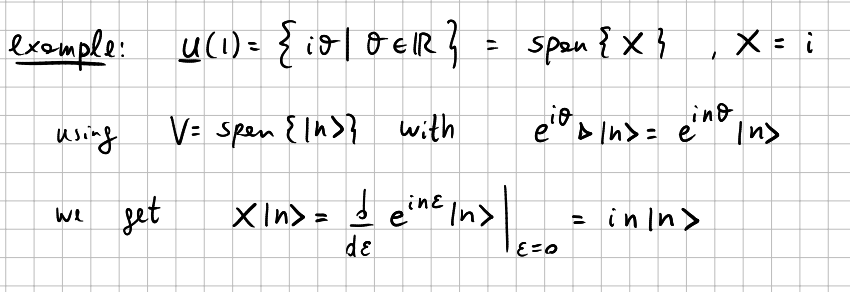
\includegraphics[scale=0.4]{lie4}
		\caption{Giuseppe's notes}
	\end{figure}
\end{exmp}


\newpage
\begin{exmp}
	
	\begin{figure}[!htb]
		\centering
		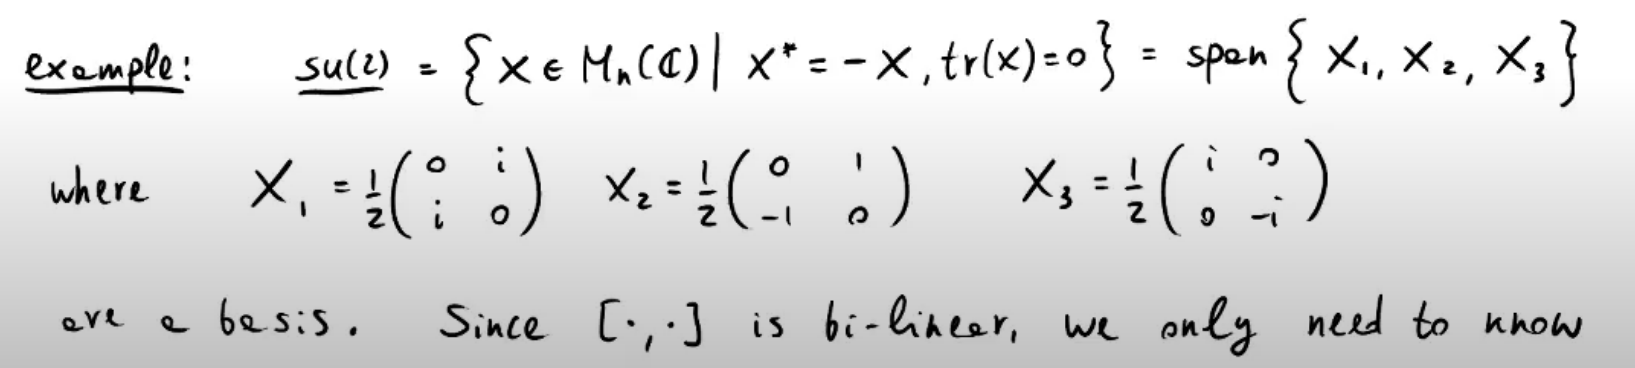
\includegraphics[scale=0.3]{lie5}
		\caption{Giuseppe's notes}
	\end{figure}
\end{exmp}










\newpage
\section{Symmetries in quantum mechanics}


\begin{thm}[Wigner's Theorem]  If $T : H \to H$ is an invertible transformation of an Hilbert space into itself that preserves transition amplitudes
\begin{align}
\f{\abs{\la T(\psi),  T(\phi) \ra }^2}{\norm{T\psi}^2\norm{T\phi}^2} = \f{\abs{\la \psi,\phi \ra}^2}{\norm{\phi}^2 \norm{\psi}^2}
\end{align}	
for all $\phi,\psi \in H$ then one of the following happens:
\begin{itemize}
	\item $T$ is linear an unitary (up to a multiplicative constant)
	\item $T$ is anti-linear and anti-unitary (up to a multiplicative constant).
\end{itemize}
	
	
\end{thm}


Since symmetries, at the very least, preserve transition amplitudes, they should act as unitary or anti-unitary operators. \\

Since the identity is unitary, if $G$ is a connect group of symmetries, by continuity $G$ must act unitarily. \\

\textbf{Note:} Anti-unitary ones are used for time reversal, and all these sound like unitary representations!\\


Now, back to representations, if $V$ is a $G$-module, we can make it into a Lie$(G)$-module by defining 
\begin{align}
X \triangleleft \ket{\psi} = \f{d}{d\ep}\lp e^{\ep X} \triangleleft\ket{\psi} \rp\bigg\vert_{\ep=0} = \lim_{\ep=0}\f{1}{\ep}\lp e^{\ep X}\triangleleft\ket{\psi} - e^{0X}\triangleleft\ket{\psi} \rp.
\end{align}


\begin{exmp}
	If $U(1)$ acts on $V_n = \text{span}\{ \ket{n}   \}$ as $e^{i\theta}\triangleleft\ket{n} = e^{in\theta}\ket{n}$ and $i = (d/d\ep)\vert_{\ep=0} e^{i\ep} \in \mathfrak{u}(1)$, then 
	\begin{align}
	i\triangleleft\ket{n} = \dots = in\ket{n}
	\end{align}
	which is indeed an action of $\mathfrak{u}(1)$. Note that the action of $\mathfrak{u}(1)$ is anti-hermitian. So we have a $\mathfrak{u}(1)$-module.
\end{exmp}







Now, we ask, Does the converse work? In other words, do all the representations of Lie$(G)$ come from representations of $G$? Well, suppose we have a new class of representations $V_a = \text{span}\{ \ket{a} \}, a \in \R$ with the action $U(1): i\triangleleft\ket{a} = ia\ket{a}$. This is a unitary $\mathfrak{u}(1)$-module, since
\begin{align}
\overline{\bra{a} i\triangleleft\ket{a} } = \dots = -\bra{a}i\triangleleft\ket{a},
\end{align} 
which we see is anti-hermitian. Can we say that 
\begin{align}
e^{i\theta} \triangleleft\ket{a} = ``\exp\lb i\theta \triangleleft \ket{a} \rb''?
\end{align}
which is the reverse of $i\theta \triangleleft \ket{n} = (d/d\ep)\vert_{\ep=0} e^{\ep X}\triangleleft \ket{a} $. Suppose we say that 
\begin{align}
e^{i\theta}\triangleleft\ket{a} = \sum^\infty_{n=0} \f{(i\theta)^n}{n!} \triangleleft \ket{a}.
\end{align}
With this, we can see that
\begin{align}
\sum^\infty_{n=0} \f{(i\theta)^n}{n!} \triangleleft \ket{a} = \lp \sum^\infty_{n=0} \f{(i a \theta)^n}{n!} \rp \ket{a} = e^{i\theta a}\ket{a}.
\end{align}
So can we say
\begin{align}
e^{i\theta}\triangleleft \ket{a} = e^{i\theta a}\ket{a}?
\end{align}
The answer is NO. One thing we did that doesn't make sense is this; The mistake is the ambiguity of 
\begin{align}
e^{i\theta} \triangleleft\ket{a} = \exp\lb i\theta \triangleleft \ket{a} \rb
\end{align}
because the choice of $\theta$ is ambiguous $e^{i\theta} = e^{i\theta + i 2\pi k}$. To make this clear, we need to make a choice, say $\theta \in (-\pi, \pi]$. So, we must say that if $z\in U(1), z\triangleleft \ket{a} = e^{ia \arg(z)}\ket{a}$. \\

Now, all seems well. Is this a $U(1)$-module? 
\begin{itemize}
	\item It is linear.
	\item The problem arises in this next item because $\arg(z) + \arg(w)  = \arg(z+w)+ 2\pi k$: 
	\begin{align}
	e^{ia(\arg(z) + \arg(w))} = e^{ia(\arg(z) + \arg(w))} e^{i2\pi a k}.
	\end{align}
	This last term is not one in general. If $a = 1/2$, then we end up with 
	\begin{align}
	e^{i\pi}\triangleleft e^{i\pi} s\triangleleft \ket{1/2} = -\ket{1/2} \neq e^{i\pi} e^{i\pi}\ket{a} = \ket{1/2}.
	\end{align}
	Now, is everything broken? We see that whether things work depends on the value of $a$. It turns out that NOTHING has been broken! Remember that physical states are only defined up to a non-zero scalar $(\ket{\psi} \sim \lambda \ket{\psi})$ if $\lambda \neq 0$. We have equivalence classes!
	\begin{align}
	[e^{i\pi}\triangleleft e^{i\pi}\triangleleft \ket{1/2}] = [-\ket{1/2}] = [\ket{1/2}] = [e^{i2\pi }\triangleleft \ket{1/2}]. 
	\end{align} 
	And thus we have in general, $z\triangleleft z \triangleleft \ket{a} = (zw)\triangleleft \ket{a}$. We call these equivalence classes \textit{projective representations}. In general, we will have that
	\begin{align}
	g\triangleleft h \triangleleft \ket{\psi} = e^{i\omega(g,h)} (gh)\triangleleft \ket{\psi}
	\end{align}
	still describes a symmetry. 
\end{itemize}




\begin{prop}[Nice things that happen] Suppose $V$ is finite-dimensional. 
	\begin{itemize}
		\item The projective representations of $G$  are all obtained by ``exponentiating'' pure representations of Lie$(G)$ ($G$ connected) -- pure in the sense that they are not projective. 
		\begin{itemize}
			\item Pure representations of Lie$(G)$ instead of projective representations of $G$. 
			\item Representations of Lie$(G)$ are easier to find then representations of $G$. 
		\end{itemize}  
	
	
		\item Projective representations of $G$ are in ``one-to-one'' correspondence with pure representations of $\tilde{G}$ where ($\tilde{G}$ is a simply connected cover of $G$). 
		\begin{exmp}
			$\tilde{SO}(3) = SU(2)$. 
		\end{exmp}
		Note that simply connected covers are unique. With this, instead of looking at projective representations of $SO(3)$, we can look at representations of $SU(2)$. The pure representations of $SO(3)$ are labeled by integers, while the projective representations of $SO(3)$ are labeled by half-integers. These concepts are related to angular momentum. 
	\end{itemize}
	
\end{prop}


The idea is that, in QM, in most of what we do is related to representation theory. 



























\newpage
\section{Exercises}
\noindent \textbf{1.} Prove the following consequences of the definition of a group:
\begin{enumerate}
	\item the identity element is unique (if two elements satisfy the identity property, they are
	necessarily equal).
	
	\begin{proof}
		If $e,e'$ are identities of $G$, then $e = e'e = e'e = e'$. 
	\end{proof}
	
	\item For each $g \in G$ the inverse $g^{-1}$ is unique.
	
	\begin{proof}
		Multiplying both sides on the right by any inverse to to get $g^{-1}*g = g'^{-1}*g = e \implies g^{-1} = g'^{-1}$.
	\end{proof}
	
	\item $(g^{-1})^{-1} = g$.
	
	\begin{proof}
		$g^{-1}* (g^{-1})^{-1} = e = g^{-1}*g \implies g=(g^{-1})^{-1}$, by multiplying by $g^{-1}$ on the right on both sides. 
	\end{proof}
	
	\item $(gh)^{-1} = h^{-1}g^{-1}$.
	
	\begin{proof}
		Multiplying both sides by $gh$ we get $(gh)(gh)^{-1} = e = ghh^{-1}g^{-1}$, so we're done, by the previous items.
	\end{proof}


\end{enumerate}


\noindent \textbf{2.} Prove that if $\varphi : G \to H$ is a group homomorphism then 
\begin{enumerate}
	\item $\varphi(e_G) = e_H$. (Hint: look at $\varphi(e_G e_G)$).
	
	\begin{proof}
		$\varphi(e_G) = \varphi(e_G e_G) = \varphi(e_G)\varphi(e_G) \implies \varphi(e_G) =e_H$ (we just showed that $\varphi(e_G)$ is an identity element in $H$). 
	\end{proof}
	
	\item $\varphi(g^{-1}) = \varphi(g)^{-1}, \forall g\in G$.
	\begin{proof}
		$\varphi(e_G) = \varphi(g^{-1}g)= \varphi(g)\varphi(g^{-1}) = \varphi(g)\varphi(g)^{-1}$, so we have that $\varphi(g^{-1}) = \varphi(g)^{-1}$.
	\end{proof}
\end{enumerate}


\noindent \textbf{3.} Prove that $\mathbb{Z}_2$ is isomorphic to the subgroup $\{-\mathbb{I}_n, \mathbb{I}_n \} \leq GL(n,\mathbb{C})$. While you are at it, prove that the latter is indeed a subgroup.

\begin{proof}
	Showing the latter set is s subgroup is easy so I won't do it. Consider the group homomorphism $\varphi: \mathbb{Z}_2 \to \{ -\mathbb{I}_n, \mathbb{I}_n \}$ defined by $\varphi(0) = \mathbb{I}_n$, and $\varphi(1) = -\mathbb{I}_n$. The map is bijective by definition. By inspection, the map is also a group homomorphism. So, the map is an isomorphism. This means the two groups are isomorphic to each other. 
\end{proof}


\noindent \textbf{4.} I'll do you one better: prove that any group with only two elements is isomorphic to $\mathbb{Z}_2$.

\begin{proof}
	Call the two-element group $G = \{ g,g^{-1} \}$. Create a map just like that in the previous exercise and we're done. 
\end{proof}





\noindent \textbf{5.} Show that $2\mathbb{Z} = \{ 2n \vert n \in \mathbb{Z} \}$ is a normal subgroup of $(\mathbb{Z},+)$ and that $\mathbb{Z}_2 = \mathbb{Z} / 2\mathbb{Z}$.


\begin{proof}
	This follows almost directly from the definitions. 
\end{proof}





\noindent \textbf{6.} Prove the first isomorphism theorem.

\begin{proof}
	Refer to the Abstract Algebra \href{https://huanqbui.com/archives/MA333.pdf}{\underline{notes}} for the proof. The first two items are easy. The last item is also easy but requires a trick. $\ker\varphi$ is normal, so 
	\begin{align}
	h^{-1}g \in \ker\varphi \iff \varphi(h^{-1}g) = \varphi(h)^{-1}\varphi(g)  = e_H \implies \varphi(g) = \varphi(h).
	\end{align}
	This means that 
	\begin{align}
	[g] = \{ h\in G \vert \varphi(h) = \varphi(g)   \}. 
	\end{align}
	With these we can prove the third item. 
\end{proof}




\noindent \textbf{7. Noether's Theorem.}  Consider the Lagrangian
\begin{align}
\lag(q,\dot{q},t) = \f{1}{2}\lp m\dot{q}^2 - kq^2 \rp e^{\al t}, \quad \al \in \R
\end{align}
with the transformations
\begin{align}
\td{t} = T_\ep(t) = t+\ep, \quad \td{q} = Q_\ep(q) = qe^{-\ep\al/2}.
\end{align}

\begin{itemize}
	\item Show that $T_\ep, Q_\ep$ are one-parameter subgroups. 
	\begin{proof}
		Let's not worry about this. We only need to verify that these transformations satisfy the defining characteristics of one-parameter subgroups. Remember that one-parameter subgroups satisfy the following properties:
		\begin{itemize}
			\item $g_0 = e_G$
			\item $g_{-\epsilon} = g_\epsilon^{-1}$
			\item $g_{\epsilon + \epsilon'} = g_\epsilon g_{\epsilon'}$. This means the the one-parameter subgroup is abelian.
		\end{itemize}
	\end{proof}

	\item Show that $\delta S = (d/d\ep)\big\vert_{\ep=0}\td{S}[\td{q}] = 0$ without using the Euler-Lagrange equations, using the fact that
	\begin{align}
	\delta S = \int^b_a dt\lb \lag(q,\dot{q},t)\f{d}{dt}\delta t + \f{\p \lag}{\p t}\delta t + \f{\p \lag}{\p q}\delta q + \f{\p \lag}{\p \dot{q}}\lp \f{d}{dt}\delta q - \dot{q}\f{d}{dt}\delta t\rp \rb
	\end{align}
	and substitute $\lag, \delta t, \delta q$.
	\begin{proof}
	By definition we get $\delta t=  1$ and $\delta q = -\al q/2$. With these we get 
	\begin{align}
	\delta S = \int^b_a dt\lb \f{\p \lag}{\p t} + \f{-\al q}{2} \f{\p \lag}{\p q} + \f{\p \lag}{\p \dot{q}}\lb \dot{q}\f{-\al}{2} - 0 \rb \rb = 0.
	\end{align}
	\end{proof}

	\item Find the associated conserved quantity.
	\begin{proof}
	The associated conserved quantity is given, by definition, as
	\begin{align}
	\lag \delta t + \f{\p \lag}{\p \dot{q}}(\delta q - \dot{q}\delta t)
	\end{align}
	A simple computation gives the result. 
	\end{proof}

	\item Find the Euler-Lagrange equations
	\begin{proof}
	Remember that the Euler-Lagrange equations are given by
	\begin{align}
	\f{\p \lag}{\p q} - \f{d}{dt}\f{\p \lag}{\p \dot{q}} =0.
	\end{align}
	Simple computations give us the EOM.
	\end{proof}

	\item Show that the conserved quantity is indeed conserved if the Euler-Lagrange equations hold. 
	\begin{proof}
	This is also a simple verification, so I won't worry about it. 
	\end{proof}

	
\end{itemize}


\noindent \textbf{8.} Find out the explicit form and dimension of the Lie algebras of the following groups: $GL(n,\R), SL(n,\R), SL(n,\C), O(n), SO(n), SU(n)$. 

\begin{proof}
	For example, $U(n) = \{ A\in GL(n,\C)  \vert A^\dagger A = 1\}$. Then $\mathfrak{U}(n) = \{ X\in M_n(\C) \vert e^{\ep X}\in U(n) \forall \ep \in \R   \}$. Using properties of matrix exponentials, we find that $\mathfrak{U}(n) = \{ X\in M_n(\C) \vert X^\dagger = -X   \}$. 
	\begin{figure}[!htb]
		\centering
		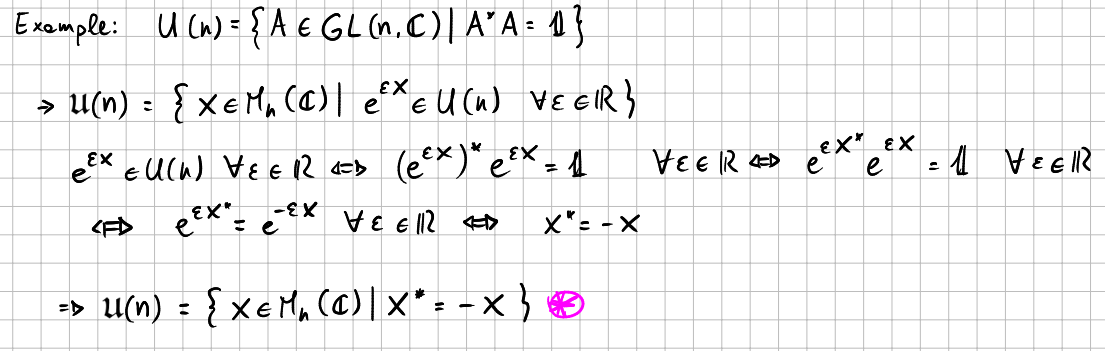
\includegraphics[scale=0.3]{lie1}
		\caption{From Giuseppe's Notes}
	\end{figure}
	
	As a real vector space, Let $X = A + iB$, then $X^\dagger = -X$ if and only if $A^\top = -A, B^\top = B$. This means the dimension is $n(n+1)/2 + n(n-1)/2 = n^2$. With this we can proceed to the other examples. It's useful to remember the following facts in the figure.
	\begin{figure}[!htb]
		\centering
		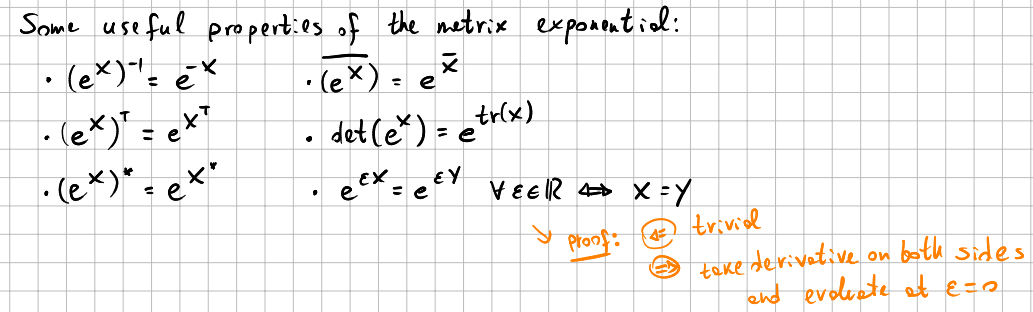
\includegraphics[scale=0.4]{lie2}
		\caption{From Giuseppe's notes}
	\end{figure}

\end{proof}



\noindent \textbf{9.} Do the same thing for 
\begin{itemize}
	\item The complex special orthogonal group: $SO(n,\C)$.
	\item Indefinite special orthogonal group: $SO(p,q)$. 
	\item Real symplectic group: $Sp(2n,\R)$.
	\item Complex symplectic group: $Sp(2n,\C)$.
	\item Compact symplectic group: $Sp(n) = Sp(2n,\C)\cap U(2n)$.
\end{itemize}
\begin{figure}[!htb]
	\centering
	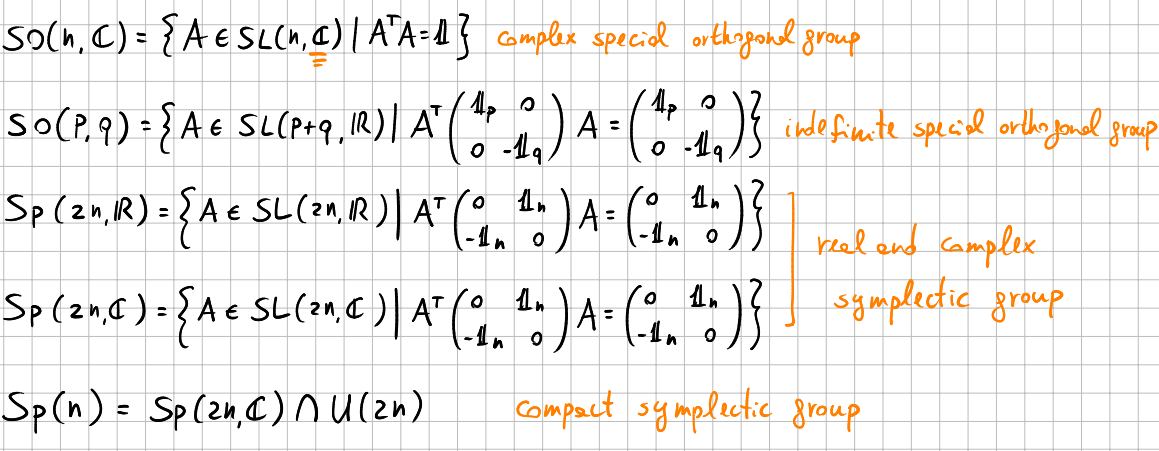
\includegraphics[scale=0.4]{lie3}
	\caption{From Giuseppe's notes}
\end{figure}


\begin{proof}
	For example,
	\begin{figure}[!htb]
		\centering
		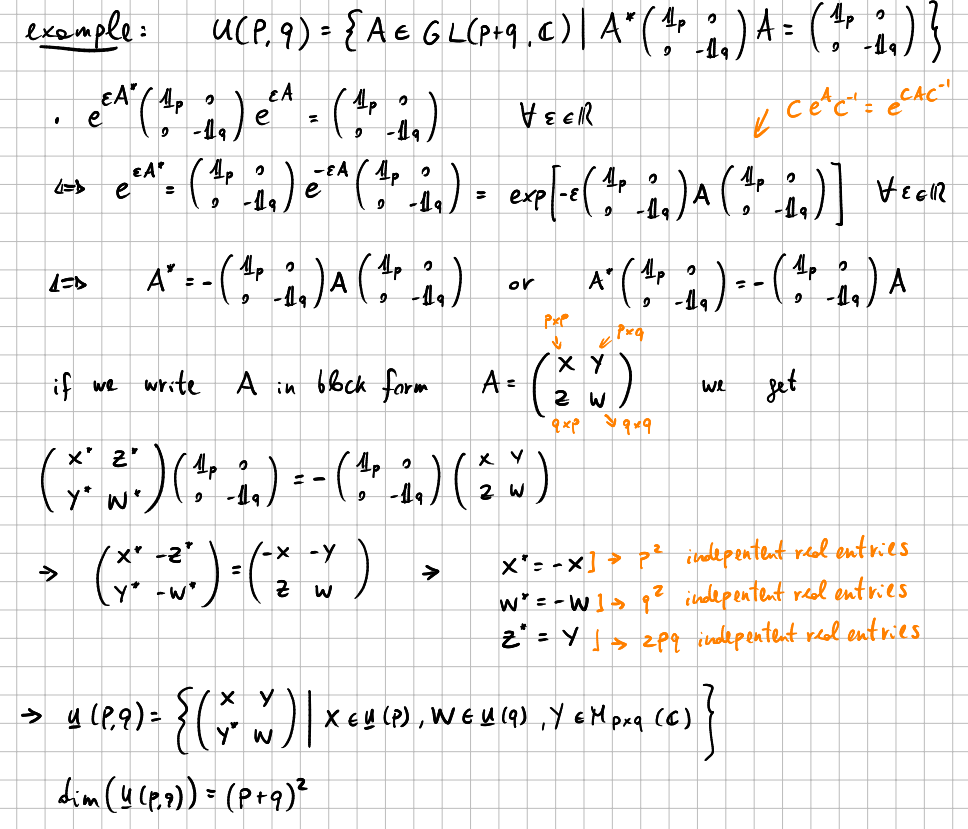
\includegraphics[scale=0.4]{lie}
		\caption{From Giuseppe's notes}
	\end{figure}
\end{proof}
































\newpage



\chapter{Research Project: Quantum Simulation}

\textbf{Quantum many-body physics on quantum hardware}\\


\underline{Project description:} Recently, there have been significant advances in several quantum computing platforms, including superconducting qubits and trapped ions. At this point, nontrivial quantum operations can be implemented
on tens of qubits, and the frontier continues to expand. This project will explore how these emerging
technologies can assist the realization and understanding of complex many-body quantum systems,
regarding both static aspects such as ground state properties and dynamical aspects such as quantum chaos
and thermalization. What new physics can we learn from near-term quantum computers? The ideal
outcome is an interesting and realistic proposal that can be carried out in one of the quantum platforms (see
for example the interplay between theoretical proposals and experiment).














\newpage


\section{Review: The density operator}        

  
We often use the language of state vectors in quantum mechanics. An alternative language is that of \textit{density matrices/density operators}. We will use this language extensively in quantum information/quantum computation. First, we will introduce the formulation. Second, we look at some properties of the density operator. Finally, we look at an application where the density operator really shines -- as a tool for describing \textit{individual subsystems} of a composite quantum system.  


\subsection{Ensembles of Quantum States}

The density operator language provides a convenient means for describing quantum systems whose state is not completely known. Suppose a quantum system is in one of the states $\ket{\psi_i}$ where $i$ is an index, with respective probabilities $p_i$. We call $\{p_i, \ket{\psi_i}\}$ an \textit{ensemble of pure states}. \\

\begin{defn}[Density Operator]
	\begin{align}
	\boxed{\rho \equiv \sum_i p_i \ket{\psi_i}\bra{\psi_i}}
	\end{align}
\end{defn}



Suppose we let a unitary $\U$ act on a closed system. If the system was initially in the state $\ket{\psi_i}$ with probability $p_i$ then we get $\U \ket{\psi_i}$ with probability $p_i$. The density operator evolves as
\begin{align}
\rho = \sum_i p_i \ket{\psi_i}\bra{\psi_i} \stackrel{\U}{\rightarrow} \sum_i p_i \U \ket{\psi_i}\bra{\psi_i}\U^\dagger = \U \rho \U^\dagger.
\end{align}


Suppose we have a measurement gate $\M_m$. If the intial state is $\ket{\psi_i}$ then the probability of getting result $m$ is 
\begin{align}
p(m\vert i) = \bra{\psi_i} \M_m^\dagger \M_m \ket{\psi_i} = \tr\lp \M_m^\dagger \M_m \braket{\psi_i} \rp
\end{align}
where we have used the identity:
\begin{align}
\tr(A\ket{\psi}\bra{\psi}) = \sum_i \bra{i}A \ket{\psi}\bra{\psi}\ket{i} = \bra{\psi}A\ket{\psi}.
\end{align}
With this, the total probability of measuring $m$ is 
\begin{align}
p(m) = \sum_i p(m|i)p_i = \sum_i p_i \tr\lp \M_m^\dagger \M_m \ket{\psi_i}\bra{\psi_i} \rp = \tr\lp \M_m^\dagger \M_m \rho \rp.
\end{align}

The state after the measurement is thus
\begin{align}
\ket{\psi_i^m} = \f{\M_m \ket{\psi_i}}{\sqrt{\bra{\psi_i}\M_m^\dagger \M_m \ket{\psi_i}}}.
\end{align}
The corresponding density operator for this state is thus
\begin{align}
\rho_m = \sum_i p(i|m)\ket{\psi_i^m}\bra{\psi_i^m} = \sum_i p(i|m)\f{\M_m \ket{\psi_i}\bra{\psi_i}\M_m^\dagger}{\bra{\psi_i}\M_m^\dagger \M_m \ket{\psi_i}}.
\end{align}
From probability theory we have $p(i|m) = p(m|i)p_i/p(m)$, so:
\begin{align}
\rho_m = \sum_i p_i \f{\M_m \ket{\psi_i}\bra{\psi_i}\M_m^\dagger}{\tr\lp \M^\dagger_m \M_m \rho \rp} = \f{\M_m \rho \M_m^\dagger}{\tr\lp \M_m^\dagger \M_m \rho \rp}.
\end{align}




Finally, suppose we have a quantum system in state $\rho_i$ with probability $p_i$. The system might be described by the density matrix
\begin{align}
\rho = \sum_i p_i \rho_i.
\end{align}
Here's why:
\begin{align}
\rho = \sum_{i,j}p_i p_{ij}\ket{\psi_{ij}}\bra{\psi_{ij}} = \sum_i p_i \rho_i
\end{align}
where we have used the definition
\begin{align}
\rho_i = \sum_{j}p_{ij}\ket{\psi_{ij}}\bra{\psi_{ij}}.
\end{align}

We call $\rho$ the \textit{mixture} of the states $\rho_i$ with probabilities $p_i$. This concept of mixture comes up up repeatedly in the analysis of problems like quantum noise, where the effect of the noise is to introduce ignorance into our knowledge of the quantum state. A simple example is provided by the measurement scenario. Imagine that for some reason out record of the result $m$ of the measurement was lost. We would have a quantum system in the state $\rho_m$ with probability $p(m)$, but would no longer know the actual value of $m$. The state of such a quantum system would therefore by described by the density operator
\begin{align}
\rho = \sum_m p(m)\rho_m = \sum_m \tr\lp \M_m^\dagger \M_m \rho \rp\f{\M_m \rho \M_m^\dagger}{\tr\lp \M_m^\dagger \M_m \rho \rp} = \sum_m \M_m \rho \M_m^\dagger.
\end{align}






























\subsection{General Properties of the Density Operator}



\begin{thm}[Characterization of density operators] 
	An operator $\rho$ is the density operator to some ensemble $\{p_i, \ket{\psi_i} \}$ if and only if it statisfies the conditions
	\begin{itemize}
		\item \textbf{Trace condition:} $\tr(\rho) = 1$.
		\item \textbf{Positivity:} $\rho$ is a positive operator, i.e., $\bra{\varphi}\rho\ket{\varphi} \geq 0 \forall \varphi$.
	\end{itemize}
\end{thm}


With this definition we can reformulate the postulates of quantum mechanics in the language of density operators as 
\begin{itemize}
	\item \textbf{Postulate 1:} Associated to any isolated physical system is a Hilbert space known as the \textit{state space} of the system. The system is completely described by its \textit{density operator}, which is a positive operator $\rho$ with trace one, acting on the state space of the system. If a quantum system is in the state $\rho_i$ with probability $p_i$ then the density operator for the system is $\sum _i p_i \rho_i$.
	
	\item \textbf{Postulate 2:} The evolution of a \textit{closed} quantum system is described by a \textit{unitary transformation}:
	\begin{align}
	\rho' = \U \rho \U^\dagger.
	\end{align} 
	
	
	
	\item \textbf{Postulate 3:} Measurements are described by a collection $\{\M_m\}$ of \textit{measurement operators}. The index $m$ refers to the measurement outcomes that may occur. If the state of the quantum system is $\rho$ immediately before the measurement then the probability that result $m$ occurs is given by
	\begin{align}
	p(m) = \tr\lp \M_m^\dagger  \M_m \rho_m \rp
	\end{align}
	and the state of the system after the measurement is 
	\begin{align}
	\f{\M_m \rho \M_m^\dagger}{\tr\lp \M_m^\dagger \M_m \rho \rp}.
	\end{align}
	The measurement operators satisfy the completeness equation
	\begin{align}
	\sum_m \M_m^\dagger \M_m = \Id.
	\end{align}
	
	
	
	\item \textbf{Postulate 4:} The state space of a composite physical system is the tensor product of the state spaces of the component physical systems. E.g. the joint state of the total system can be written as $\rho_1 \otimes \dots \otimes \rho_n$.
\end{itemize}



\begin{thm}[Pure states] 
	$\tr(\rho^2) \leq 1$. Equality occurs if and only if $\rho$ is a pure state. 
\end{thm}



\begin{thm}[Unitary freedom in the ensemble for density matrices] 
	The sets $\ket{\tilde{\varphi}_i}$ and $\ket{\tilde{\psi}_j}$ generate the same density matrix if and only if they are unitarily similar, i.e., 
	\begin{align}
	\ket{\tilde{\varphi}_i} = \sum_{j} u_{ij}\ket{\tilde{\psi}_j}
	\end{align}
	where the $u_{ij}$ are entries of a unitary $\U$.
	
\end{thm}




\subsection{The Reduced Density Operator}
Te deepest application of the density operator is as a descriptive tool for \textit{sub-systems} of a composite quantum system. Such a description is given by the \textit{reduced density operator}. \\

Suppose we have physical systems $A$ and $B$ whose state is described by the density operator $\rho^{AB}$. The reduced density operator for $A$ is then given by
\begin{align}
\rho^A = \tr_B\lp \rho^{AB} \rp
\end{align}
where $\tr_B$ is the \textit{partial trace} over system $B$, defined by    
\begin{align}
\tr_B\lp \ket{a_1}\bra{a_2} \otimes \ket{b_1}\bra{b_2} \rp \equiv \ket{a_1}\bra{a_2}\tr\lp \ket{b_1}\bra{b_2} \rp = \ket{a_1}\bra{a_2}\braket{b_2}{b_1}
\end{align}
where $\ket{a_1}, \ket{a_2}$ are any two vectors in the state space of $A$, and $\ket{b_1}, \ket{b_2}$ are any two vectors in the state space of $B$. \\




\begin{exmp}
	To understand this construction, consider an example where $\rho^{AB} = \rho \otimes \sigma$ where $\rho,\sigma$ describe $A,B$ respectively. Then
	\begin{align}
	\rho^A = \tr_B\lp \rho \otimes \sigma \rp = \rho \tr(\sigma) = \rho
	\end{align}
	as expected. 
\end{exmp}




\newpage








\section{Quantum Computational Complexity: An Introduction}

In this section we look at quantum computational complexity, as introduced in this \href{https://arxiv.org/pdf/0804.3401v1.pdf}{\underline{paper}} by John Watrous at the IQC, the University of Waterloo.

\subsection{Introduction}

\begin{itemize}
	\item \textbf{P}
	
	\item \textbf{NP}
	
	
	\item \textbf{BPP}
	
	\item \textbf{PP}
	
	\item \textbf{MA}
	
	
	\item \textbf{AM}
	
	\item \textbf{SZK}
	
	\item \textbf{PSPACE}
	
	\item \textbf{EXP}
	
	\item \textbf{NEXP}
	
	
	\item  \textbf{PL}
	
	\item \textbf{NC}
\end{itemize}

\begin{figure}[!htb]
	\centering
	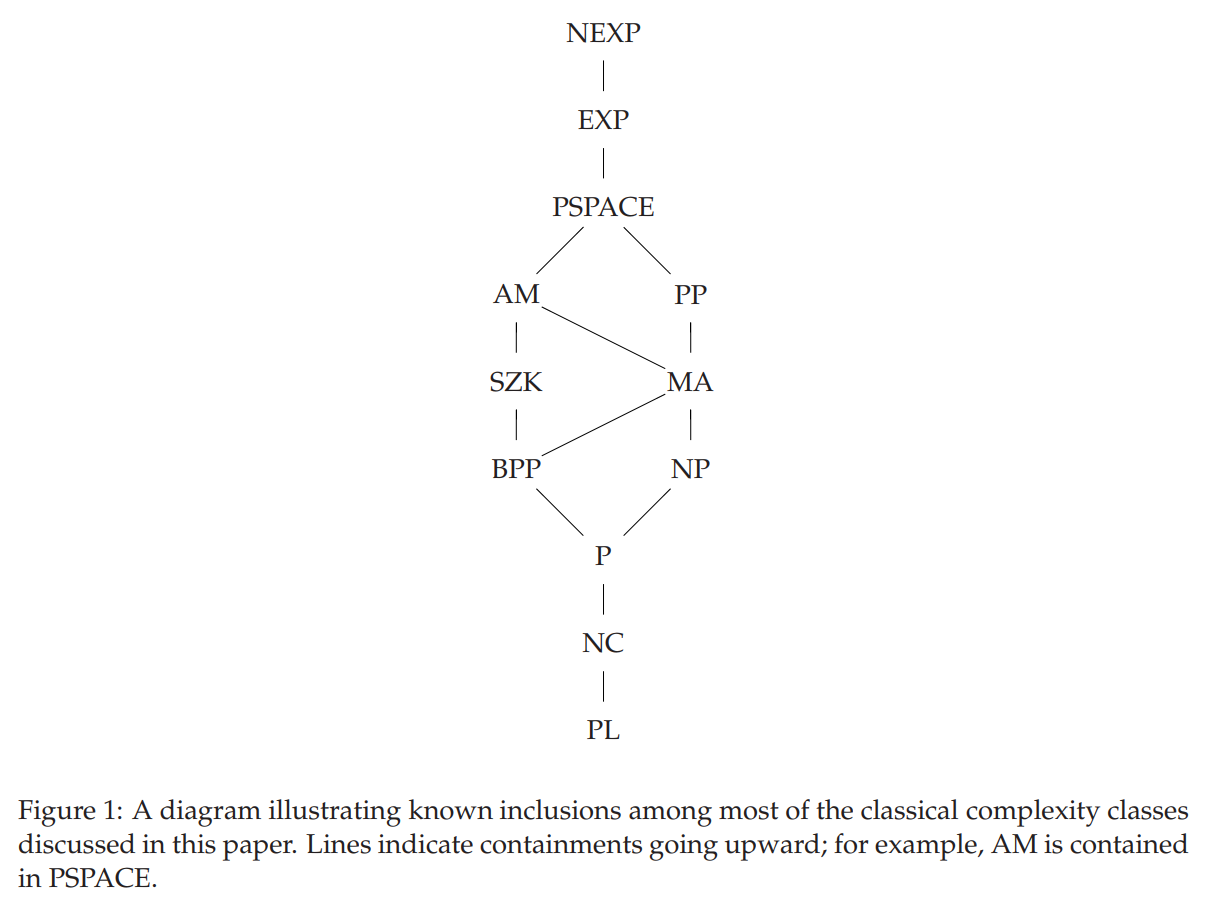
\includegraphics[scale=0.3]{complexity}
\end{figure}










\newpage






\section{Quantum Simulation: A Primer}

Here's what Feynman said in 1982:\\

\textit{``Can physics be simulated by a universal computer? [...] the physical world is quantum mechanical, and therefore the proper problem is the simulation of quantum physics [...] the full description of quantum mechanics for a large system with $R$ particles [...] has too many variables, it cannot be simulated
with a normal computer with a number of elements proportional to $R$ [ ... but it can be simulated with ] quantum computer elements. [...] Can a quantum system be probabilistically simulated by a classical (probabilistic, I'd assume) universal computer? [...] If you take the computer to be the classical kind I've described so far [..] the answer is certainly, No!''}


\subsection{Simulation in action}

The heart of simulation is the solution of differential equations which capture the physical
laws governing the dynamical behavior of a system. The goal is generally: given an initial state of the system, what is the state at some other time and/or position? Solutions are usually obtained by \textit{approximating} the state with a digital representation, then \textit{discretizing} the differential
equation in space and time such that an iterative application of a procedure carries the state from the initial to the final conditions.\\

The error in this procedure is \textit{bounded}, and known not to grow faster than some small power of the number of iterations. Furthermore, not all dynamical systems can be simulated efficiently: generally, only those systems which can be described efficiently can be simulated efficiently.\\

Simulating quantum systems using classical computers is usually inefficient. The dynamical behavior of many simple quantum systems is governed the SE:
\begin{align}
i\hbar \p_t \ket{\psi} = \had \ket{\psi}.
\end{align}
We will set $\hbar =1$.  For real particles in space, we often have
\begin{align}
i\p_t \psi(x) = \lb -\f{1}{2m}\p_x^2 + V(x) \rb \psi(x).
\end{align}

The key challenge in simulating quantum systems is the \textit{exponential} number of differential equations which must be solved. For 1 qubit evolving according to the
SE, a system of 2 differential equations must be solved; for 2
qubits, 4 equations; and for $n$ qubits, $2^n$ equations. Sometimes, insightful approximations can be made which reduce the effective number of equations involved, but there are many physically interesting quantum systems for which no such approximations are known.
\\

There are many important quantum systems for which classical simulation is intractable. For example:
\begin{align}
\mbox{Hubbard model: } \had = \sum^n_{k=1}V_0 n_{k^\uparrow}n_{k\downarrow} + \sum_{k,j\mbox{ neighbors,}\sigma} t_0 c_{k\sigma}^* c_{j\sigma}.
\end{align}
\begin{align}
\mbox{Ising mode: } \had = \sum_{k=1}^n \vec{\sigma_k}\cdot \vec{\sigma}_{k+1} .
\end{align}
Quantum computers can efficiently simulate quantum systems for which there is no known efficient classical simulation.












\subsection{The quantum simulation algorithm}

The quantum simulation is concerned with the solution of $i \p_t \ket{\psi} = \had \ket{\psi}$, which, for a time-independent $\had$, is just
\begin{align}
\ket{\psi(t)} = e^{-i\had t}\ket{\psi(0)}.
\end{align}
$\had$ is in general difficult to exponentiate, but a good beginning is the first order solution 
\begin{align}
\ket{(\psi(t+\Delta t))} \approx (\Id - i\had \Delta t)\ket{\psi(t)}.
\end{align}
This is tractable, but often is not very satisfactory. \\

Efficient approximations to higher oder is possible for many \textit{classes} of Hamiltonians. For example, in most physical systems, the Hamiltonian can be written as a sum over many \textit{local} interactions. For a system of $n$ particles:
\begin{align}
\had = \sum^L_{k=1}\had_k \sim \bigoplus^L_{k=1}\had_k
\end{align} 
where each $\had_k$ acts on at most a constant $c$ number of systems, and $L$ is a polynomial in $n$. For instance, the terms $\had_k$ are often just 2-body interactions such as $X_i X_j$ and 1-boy Hamiltonians such as $X_i$. Note that both the Hubbard and Ising models have Hamiltonians of this form. There are sometimes additional global symmetry constraints such as particle statistics.\\

Note that although $e^{-i\had t}$ is difficult to compute, $e^{-i\had_k t}$ acts on a much smaller subsystem, and is straightforward to approximate using quantum circuits. However, because $[\had_j, \had_k] \neq 0$ in general (obviously, they don't commute in general), $e^{-i\had t} \neq \prod_k e^{-i \had_k t}$. So, we might want to ask how $e^{-i\had_k t}$ be useful in constructing $e^{-i\had t}$. \\

\textbf{Remarks:}
\begin{itemize}
	\item If the $\had_i$'s commute, then we do have $e^{-i \had t} = \prod_k e^{-i \had_k t}$. 
	
	\item The restriction of $\had_k$ to involve at most $c$ particles \textit{implies} that in the sum of the Hamiltonians, $L$ is upper bounded by a polynomial in $n$. 
\end{itemize}



The heart of quantum simulation algorithms is the following asymptotic approximation theorem:
\begin{thm}[Trotter formula]
	Let $A$ and $B$ be Hermitian operators. Then for any real $t$, 
	\begin{align}
	\lim_{n\to \infty}\lp e^{-iAt/n}e^{iBt/n} \rp^n = e^{i(A+B)t}.
	\end{align}\qed
\end{thm}



Of course, the theorem holds even if $A$ and $B$ don't commute. For now, we only consider the cases where $A,B$ are Hermitian. But $A,B$ can actually be generators of certain kinds of semigroups, which correspond to general quantum operations.\\

Using the theorem (and the proof of the theorem, which I won't show here), we can get
\begin{align}
e^{i(A+B)\Delta t} = e^{iA \Delta t}e^{i B\Delta t} + \mathcal{O}(\Delta t^2).
\end{align}
Similarly, 
\begin{align}
e^{i(A+B)\Delta t} = e^{iA\Delta t/2}e^{iB \Delta t}e^{iA \Delta t/2} + \mathcal{O}(\Delta t^3). 
\end{align}







\begin{exmp}[Hamiltonian simulation \& Trotterization, taken from \href{https://vtomole.com/blog/2019/04/07/trotter}{\underline{here}} ]
	
	The evolution of quantum system is governed by the SE $i \p_t \ket{\psi} = \had \ket{\psi}$. The solution to the SE:
	\begin{align}
	\ket{\psi(t)} = e^{-i \had t}\ket{0}
	\end{align}
	is a description on what state a system will be in after a Hamiltonian has been applied to it for a certain period of time. The problem of Hamiltonian simulation is thus states as: given a Hamiltonian $\had$ and an evolution time $t$, \textbf{output a sequence of computational gates} that implement $\U = e^{-i \had t}$.\\
	
	Hamiltonians are Hermitian operators that are usually a sum of a large number of individual Hamiltonians $\had_j$. For example, $\had = H_1 + H_2$. This sum of 2 Hamiltonians (which don't necessarily commute) can be described by the Trotter formula or the Lie product formula:
	\begin{align}
	e^{-i(H_1 + H_2)t} = \lim_{N\to \infty}\lp e^{-i H_1 t/N}e^{-iH_2 t/N} \rp^N.
	\end{align}
	Since the limit of this formula is infinite, we have to truncate the series when implementing this formula on a quantum compute. The truncation introduces error in the simulation that we can bound by $\epsilon$ such that $\norm{e^{-i \had t} - \U} \leq \epsilon$, where $\norm{\cdot}$ is some operator norm. This truncation is known as \textbf{Trotterization} and it's widely used to simulate non-commuting Hamiltonians on quantum computers. The \textbf{Trotterization formula} is then
	\begin{align}
	e^{-i \had t} = \lp e^{-iH_0 t/r}e^{-i H_1 t/r} \dots e^{-iH_{d-1}t/r}  \rp^r + \mathcal{O}(\text{polynomial factors}).
	\end{align} 
	Consider for example the Hamiltonian
	\begin{align}
	\had = X_0 + Y_1 + Z_2
	\end{align}
	where $X,Y,Z$ are Pauli matrices and the subscripts label  the qubits that the Hamiltonians act on. We can't simulate each Hamiltonian separately because they don't commute. This is why we use Trotterization where we evolve the entire Hamiltonian via repeatedly switching between evolving $X_0, Y_1, Z_2$ each for a small period of time.\\
	
	The first step in deriving the circuit that will simulate this Hamiltonian is finding the quantum gates that implement each of its individual term (so that we can make $\ket{\psi(t)}= e^{-i\had t}\ket{0}$ from $\ket{0}$ -- in a sense we want to find the correct form for $e^{f(X_0)}$). It turns out that this is easy since the quantum gates
	\begin{align}
	R_x(\theta) = e^{-i\theta X/2}, \quad R_y(\theta) = e^{-i\theta Y/2}, \quad R_z(\theta) = e^{-i\theta Z/2}
	\end{align} 
	will implies the individual terms perfectly. $\theta$ here denotes an \textbf{angle}, but we can also think of it as \textbf{time} because $\theta$ specifies the angle by which to rotate the state in a specified axis, which is synonymous with time in the sense that it specifies how ``long'' the rotation is applied on the state. \\
	
	
	Since we don't care too much about the simulation error in this example we will use  $r=2, t=1$ in the Trotter formula to get
	\begin{align}
	e^{-i(X_0 + Y_1 + Z_2)} = \lp e^{-iX_0/2}e^{-iY_1/2}e^{-iZ_2/2}\rp\lp e^{-iX_0/2}e^{-iY_1/2}e^{-iZ_2/2}  \rp
	\end{align}
\end{exmp}















\subsection{The algorithm}

\begin{itemize}
	\item \textbf{Inputs:} (1) A Hamiltonian $\had = \sum_k \had_k$ acting on an $N$-dimensional system, where each $\had_k$ acts on a small subsystem of size independent of $N$, (2) an initial state $\ket{\psi_0}$, of the system at $t=0$, (3) a positive, non-zero accuracy $\delta$, and (3) a time $t_f$ at which the evolved state is desired. 
	
	
	\item A state $\ket{\tilde{\psi}(t_f)}$ such that
	\begin{align}
	\abs{\bra{\tilde\psi (t_f)} e^{-i \had t_f} \ket{\psi_0}}^2 \geq 1 - \delta.
	\end{align}
	
	
	\item Choose a representation such that the state $\ket{\tilde\psi}$ of $n = \mbox{poly}(\log N)$ qubits approximates the system and the operators $e^{- \had_k \Delta t}$ have efficient quantum circuit approximations. Selection an approximation method and $\Delta t$ such that the expected error is acceptable, construct the corresponding quantum circuit $\U_{\Delta t}$ fo the iterative step, and do the following:
	\begin{itemize}
		\item Initialize state: $\ket{\tilde \psi_0} \leftarrow \ket{\psi_0}; j = 0.$ 
		\item Iterative update: $\to \ket{\tilde \psi_{j+1}} = \U_{\Delta t}\ket{\tilde \psi_j}$.
		\item Loop: $\to j = j+1;$ go to the second step until $j\Delta t \geq t_f$.
		
		\item Final result: $\to \ket{\tilde \psi(t_f)} = \ket{\tilde \psi}$.
	\end{itemize}
\end{itemize}


\begin{thm}[Baker-Campbell-Hausdorf formula]
	\begin{align}
	e^{(A+B)\Delta t} = e^{A \Delta t}e^{B \Delta t}e^{-(1/2)[A,B]\Delta t^2} + \mathcal{O}(\Delta t^3). 
	\end{align}
\end{thm}


\begin{proof}
	The proof is quite easy. Just, by definition, expand things out in power series. \qed
\end{proof}




\subsection{An illustrative example}

We have seen the case where the Hamiltonian is a sum of local interactions. However, this is not a fundamental requirement. Efficient quantum simulations are possible even for Hamiltonians which act non-trivially on all or nearly all parts of a large system. \\

Consider the Hamiltonian
\begin{align}
\had = Z_1 \otimes Z_2 \otimes \dots \otimes Z_n
\end{align}
which acts on an $n$ qubit system. This can be simulated efficiently. What we desire is a simple quantum circuit which implements $e^{-i \had \Delta t}$, for arbitrary values of $\Delta t$. A circuit that does this is given by
\begin{figure}[!htb]
	\centering
	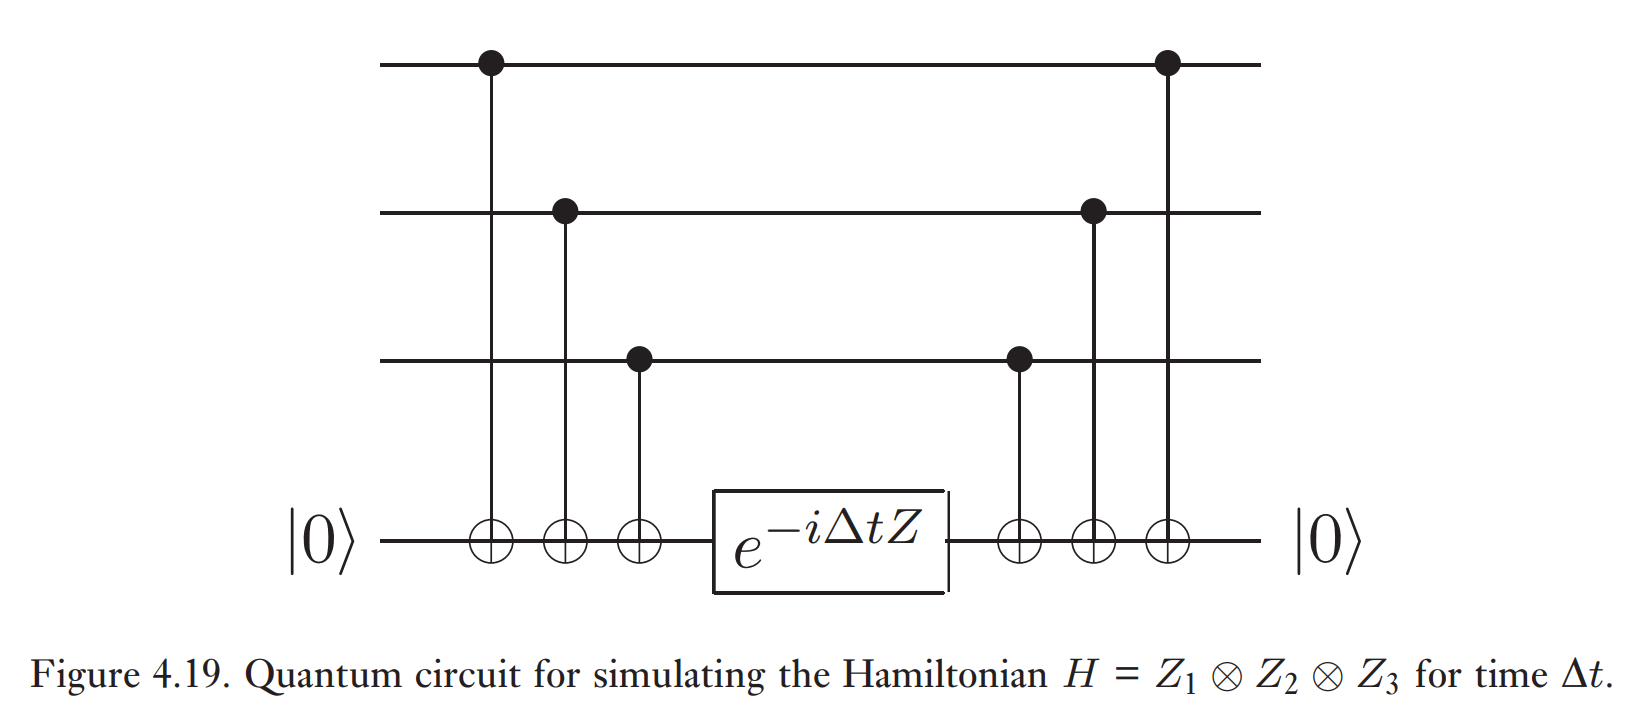
\includegraphics[scale=0.25]{qs1}
\end{figure}

Even though the Hamiltonian involves all the qubits in the system, it does so in a \textit{classical} manner: the phase shift applied to the system is $e^{-i\Delta t}$ if the \textit{parity} of the $n$ qubits in the computational basis is even. else the phase shift would be $e^{i\Delta t}$. Thus, a simple simulation of $\had$ is possible by first classical computing the parity, then applying the appropriate phase shift conditioned on the parity, then uncomputing the parity. \\

Extending the same procedure allows us to simulate more complicate extended Hamiltonians. Specifically, we can efficiently simulate any Hamiltonian of the form
\begin{align}
\had = \bigotimes^n_{k=1}\sigma^k_{c(k)}
\end{align}
where $\sigma^k_{c(k)}$ is a Pauli matrix (or identity) acting on the $k$th qubit, with $c(k) \in \{0,1,2,3\}$ specifying one of $\{I,X,Y,Z\}$. The qubits upon which the identity acts can be disregarded, and $X$ or $Y$ terms can be transformed by single qubit gates to $Z$ operations. This leaves a Hamiltonian of the form given above, which can be efficiently simulated. \\

Using this procedure allows us to simulate a wide class of Hamiltonians containing terms which are not local. It is possible to simulate a Hamiltonian of the form $\had = \sum^L_{k=1} \had_k$ where we only require that the individual $\had_k$ have a tensor product structure, and that $L$ is polynomial in the total number of particles $n$. 







\subsection{Perspectives on quantum simulation}

 
Quantum simulation is similar to classical methods, but differs fundamentally in many aspects. Each iteration of the quantum algorithm must completely replace the old state with a new one and there is no way to obtain any nontrivial information from an intermediate step without changing the algorithm (due to the no-cloning theorem). Furthermore, the final measurement must be chosen to provide the desired result because it collapses the entire state. \\

Another difficult problem is the simulation of equilibration processes. A system with Hamiltonian $\had$ in contact with an environment at temperate $T$ will come to thermal equilibrium in a state known as the \textit{Gibbs} state,
\begin{align}
\rho_{\text{therm}} = \f{e^{-\had/k_BT}}{\mathcal{Z}} \equiv \f{e^{-\had/k_BT}}{\tr\lp e^{-\had/k_BT} \rp}
\end{align}
where of course $\mathcal{Z}$ is the partition function. We can check that $\tr(\rho) = 1$. For now, we don't know how a quantum computer can simulate this. \\

Indistinguishability of particles also places a constraint on the state vector of a system which manifests itself in two ways: bosons and fermions. The state vector of a system of bosons remains unchanged under permutation of any two constituents. System of fermions experience a sign change in their state vector under interchange of any two constituents. Both kinds of systems can be simulate efficiently on a quantum computer. 















\newpage


\section{Problems in Quantum Simulations and Quantum Algorithms}

In this section, we will be looking at the following \href{https://arxiv.org/pdf/2001.03685.pdf}{\underline{review}} on quantum algorithms for quantum chemistry and materials science. 

\subsection{Quantum Simulation: An Overview}

\subsubsection{Introduction}

The interest in quantum computing for quantum simulations of molecules and materials stems from the fact that in many cases, the chemistry and physics of molecules and materials is best described using quantum mechanics. In the worst case, quantum simulation is exponentially hard on classical computers. Quantum computers have advantages over classical computers, but these advantages are problem-specific. \\


As we have seen before, the natural problem to solve on a quantum computer is the time evolution of a quantum system given some initial state:
\begin{align}
i\p_t \ket{\psi(t)} = \had \ket{\psi(t)}.
\end{align}
This problem, as we have pointed out, is of polynomial cost on a quantum computer, which can offer exponential speedup over classical computers. However, it is necessary to prepare the initial state, which may be difficult. In particular, preparing a low-energy state may be challenging, which naturally leas to considering other important problems:
\begin{align}
&\mbox{Ground state:} \quad \had\ket{\psi_0} = E_0 \ket{\psi_0}; \quad E_0 = \min_{\ket{\psi}}\bra{\psi}\had\ket{\psi}\\
&\mbox{Thermal averages:} \quad \langle \mathcal{A} \rangle = \f{\tr\lp \mathcal{A}e^{-\beta\had} \rp}{\tr\lp e^{-\beta\had} \rp}
\end{align} 
Ground state determination lies in complexity class QMA, a class of problems \textit{not known to be efficiently solvable in general on a quantum computer}. This means that thermal averages cannot in general be computed efficiently on a quantum computer, since in the limit of zero temperature, this problem reduces to ground-state determination. \\

To understand quantum advantage in chemistry, condensed matter physics, and quantum materials science, we must be guided by actual empirical data in the form of numerical and theoretical experiments with quantum algorithms and quantum devices on simulation problems of interest. This requires progress, of course. 



\subsubsection{Current quantum architectures}
There's \textit{analog quantum computation} and there's \textit{digital quantum computation}. Analog quantum computation was proposed by Feynman. The idea of analog quantum computation is to build a lattice of spins with tunable interactions and let it simulate physical systems. The limitation, however, is that this is quite limited because it can only simulate a certain set of physical systems. Furthermore, its accuracy is limited. \\

Digital quantum computation is more general. Digital quantum computation involves qubits and gates. One can show that with a finite set of gates, one can in principle generate arbitrary quantum evolutions to arbitrary precision. Every problem in the complexity class BQP can be mapped into a quantum program. \\


The third model of quantum computation is \textit{adiabatic quantum computation}. This model is considered equivalent to the digital version, but is less practical. We won't worry about this. 



\subsubsection{Building a circuit-based digital quantum computer}

The natural enemy of quantum computation is decoherence -- the tendency of quantum systems to decay into their classical states. We are current in the \textit{noisy intermediate-scale quantum} (NISQ) era, where qubit technologies (superconducting qubits, ion traps, etc) have reached the point where small devices of a few dozen qubits can be sufficiently isolated from decoherence to execute non-trivial quantum algorithms of a few tens to hundreds of gates. With these devices, an artificial but well-defined problem that is intractable classically is solved on a quantum computer. However, these problems are often not practical. The more important question is when a more relevant problem can be solved on a quantum computer. \\


To address large-scale problems, \textit{quantum error-correction} (QEC) is necessary. QEC leads to a distinction between \textit{logical} and \textit{physical} qubits. The former are error-corrected and encoded in the state of many physical qubits. Quantum algorithms are performed on the logical qubits, and the error-correction scheme translates the operations on logical qubits into physical operations. 



\newpage




\subsection{Simulation challenges in molecular and materials science }

In this section we look at some scientific problems of relevance to quantum simulation.

\subsubsection{Quantum chemistry}

Quantum chemistry is concerned with determining the low-lying eigenstates of the electronic Hamiltonian of a molecule. he eigenstates are determined for fixed sets of nuclear positions within the Born-Oppenheimer approximation. Determining the electronic energy as a function of nuclear position is key to understanding chemical reactivity, product distribution, and reaction rates.\\

Some examples of problems in quantum chemistry include
\begin{itemize}
	\item The chemistry of enzyme active sites
	\item Transition metal nanocatalysts an surface catalysts
	\item Light harvesting and the vision process
\end{itemize}

The basic metric is whether ground-states or low-energy eigenstate quantum algorithms yield more accurate energies than the best classical algorithms, for the problem sizes of interest. 

\subsubsection{Quantum molecular spectroscopy}


The theoretical goal is to compute the eigenstates of the nuclear SE. There are challenges, of course. First, the nuclear Hamiltonian is often not known, because interactions are mediated by electrons. Second, nuclear rotational and vibrational motion is often far from harmonic and not well approximate by simple mean-field theories. Third, even when the nuclear SE has been properly formulated, one faces the challenge of representing th eigenstates. \\

Some famous examples include:
\begin{itemize}
	\item Spectra of floppy molecules
	\item Hydrogen bonded clusters
\end{itemize}

There are similarities with the quantum chemistry problems, but the differences are more significant. The Hamiltonian is often more complicated because interactions are now many-body. Also, the number of states is often orders-of-magnitude greater. 


\subsubsection{Chemical quantum dynamics}

Chemical quantum dynamics if concerned with modeling time-dependent electronic and nuclear quantum effects in molecules. Some problems include:
\begin{itemize}
	\item Proton coupled electron transfer
	\item Vibrational dynamics in complex environments
	\item Plasmonic chemistry
\end{itemize}


There are multiple practical challenges. Some of this may be viewed as an issue of representation. In addition, the dynamical quantum state involves near continuum degrees of freedom, which makes discretizing the Hilbert space a challenging problem. 


\subsubsection{Correlated electronic structure in materials}

The goal here is to determine low-energy properties of materials such as Mott insulators. Some famous problems include:
\begin{itemize}
	\item High-temperature superconductivity
	\item Non-Fermi liquid behavior in heavy fermion compounds and fermionic systems near criticality
	\item Quantum fluctuations in two-dimensional systems
	\item Frustrated spin systems
\end{itemize}






%\subsubsection{Dynamical quantum effects in materials}












\newpage


\subsection{Challenges for quantum algorithms in quantum simulation}

\subsubsection{Overview of algorithms}

In this section, we look at the current status and theoretical and practical challenges to implement quantum algorithms for quantum problems. \\


The first step in a quantum simulation is to choose a \textit{representation} for the Hamiltonian and the states. We will examine the possibilities for different qubit representations, and open questions.\\

Quantum ground-state algorithms fall into different classes. QPE is a direct route to nearly exact eigenstate determination, but has been challenging to implement in the near-term era. On the other hand, \textit{variational quantum algorithms} provide the possibility to introduce approximations with adjustable circuit depth, which are determine via optimization, usually implemented in a hybrid-quantum classical loop. \\

While polynomial time algorithms for \textit{quantum time evolution} have been known for some time, algorithms with optimal asymptotic complexity as well as favorable scaling with error and low prefactors, remain an area of active research.




\subsubsection{Qubit representation of many-body systems}

To simulate many-body systems on a digital computer (either quantum or classical), the infinite-dimensional Hilbert space of a many-body system has to be truncated. The most direct route then is to define a finite set of \textit{basis functions} and then try to project the exact many-body Hamiltonian onto the chosen basis. The resulting discretized system is then expressed in terms of qubits. A choice of a good representation is important as it may affect the simulation cost dramatically. 


\begin{enumerate}
	\item \textit{Ab initio electronic structure qubit representations:}\\
	
	This concerns with the electronic structure. Consider the Hamiltonian that appears regularly in chemistry and physics
	\begin{align}
	\had = \sum^K_{i=1}-\f{1}{2}\laplacian + V(r_i) + \sum_{1\leq i<j\leq K}\f{1}{\abs{r_i - r_j}}
	\end{align}
	where $K$ is the number of electrons, $V$ is the potential created by atomic nuclei at a point $r$, and the last term represents the Coulomb interaction. Each electronic has $r_i \in \mathbb{R}^3$ and spin $\omega_i \in \{\uparrow, \downarrow\}$. So, the total wavefunction (for $K$ electrons) has the form $\psi = \psi(\vec{x}_1,\dots,\vec{x}_K)$ where $\vec{x}_i = (r_i,\omega_i)$. From Fermi statistic, we require that $\psi$ is anti-symmetric under a position swap.\\
	
	The first step is to approximate the electronic Hamiltonian with a simpler simulator Hamiltonian. This is usually achieved by truncate the Hilbert space of a single electron to a finite set of basis functions $\psi_1,\dots,\psi_N$. \\
	
	Electronic structure simulation algorithms are based on the \textit{first quantization method} (\href{https://journals.aps.org/prl/pdf/10.1103/PhysRevLett.79.2586}{\underline{link}}). We won't worry about this too much.\\
	
	The \textit{second quantization method} often results in simpler simulator Hamiltonian and requires few qubits. This methods is particularly well suited for quantum simulation algorithms and has been experimentally demonstrated for small molecules. Given a set of $N$ basis functions $\psi_1,\dots,\psi_N$, the second quantized simulator Hamiltonian is given by
	\begin{align}
	\had = \sum^N_{p,q=1} t_{pq}\hat{c}_p^\dagger \hat{c}_q + \f{1}{2}\sum^N_{p,q,r,s=1}u_{pqrs}\hat{c}^\dagger_p\hat{c}_q^\dagger \hat{c}_r \hat{c}_s.
	\end{align}
	Again, we're not going to worry too much about these. 
	
	
	
	
	
	
	
	\item \textit{Electronic basis functions:}\\
	
	The discretization of the electronic Hilbert space for a quantum simulation requires balancing two concerns. We need to represent the state with the smallest number of qubits, but also retain maximal Hamiltonian sparsity. \\
	
	There are two families of basis functions in wide use in quantum chemistry and quantum materials science: atomic orbital \textit{Gaussian bases} and \textit{Plane waves}. Gaussian bases are commonly used in molecular simulations due to their compactness, while plane waves are used in crystalline materials simulations. \\
	
	In Gaussian bases, linear combinations of Gaussian functions are placed at the nuclear positions. When they are place where the ground-state electron density is highest, they give a compact representation of the wavefunction for bound states. However, the Hamiltonian is not sparse, which leads to high gate counts. \\
	
	Plane waves offer greater simplicity as the accuracy of the basis is controlled by a single parameter, namely the kinetic energy cutoff. The number of plane waves needed to reach a desired accuracy is larger than th number of Gaussian states, but the Hamiltonian contains fewer terms ue to momentum conservation. \\
	
	The need to expose more sparsity in the Hamiltonian while retaining a reasonable compact wavefunction is an active area of research in both classical and quantum algorithms.  
	
	
	\item \textit{Fermions-to-qubit mappings:}\\
	
	Since the basic units of a quantum computer are qubits rather than fermions, any quantum simulation algorithm of fermions emplyos a suitable encoding of fermionic degrees of freedom into qubits. The standard \textit{Jordan-Wigner} mapping identifies each Fermi mode with a qubit such that the empty and the occupied states are mapped to the qubit basis states $\ket{0}$ and $\ket{1}$ respectively. The Jordan-Wigner mapping/transformation is a transformation that maps spin operators onto fermionic creation and annihilation operators. 
	\begin{figure}[!htb]
		\centering
		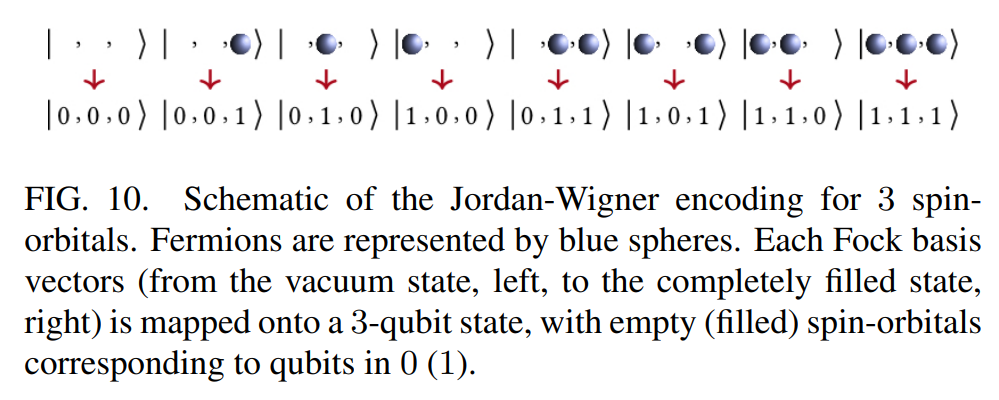
\includegraphics[scale=0.3]{jw}
	\end{figure}
	A natural question is whether the number of qubits required to express a Fermi system can be reduced by exploiting symmetries such as the particle number conservation or
	the point group symmetries of molecules. For example, zero
	temperature simulations often target only one symmetry sector containing the ground state. This motivates the study
	of \textit{symmetry-adapted fermion-to-qubit mappings}.
\end{enumerate} 



\subsubsection{Quantum algorithms for ground and excited states}

There are many approaches to obtaining ground states or
excited states on a quantum computer. State preparation
procedures attempt to construct a circuit to prepare a state
with as large as possible overlap with the desired eigenstate. One set of such procedures, which includes adiabatic state preparation and quantum imaginary time evolution, uses a prescribe evolution path. An alternative strategy is based on \textit{variational methods}, which are often called variational quantum eigensolvers. Here, the preparation circuit itself is defined via the optimization of the energy with respect to parameters of the circuit. \\


Given some state with sufficiently large overlap with the desired state, one can perform \textit{quantum phase estimation} (QPE) which simultaneously projects the state onto an eigenstate of the Hamiltonian and obtains an estimate for the energy of this eigenstate. The error, as we have seen, is inversely proportional to the simulation time. The probability of successfully projecting onto the desired state is given by the square overlap of the input state and
the desired state, and it is thus necessary to use some other
method (such as the state preparation procedures above) to
prepare an input state with sufficient overlap with the desired
state.\\


There are weaknesses to this, of course. While phase estimation allows the deviation of the final state from an exact eigenstate to be systematically reduced, it can require deep circuits with many controlled gates that are challenging for devices with limited coherence and without error correction. Variational methods replace such circuits b a large number of potentially short simulations. However, if one des not measure the energy by phase estimation, but instead by expressing the Hamiltonian as a sum of multi-qubit Pauli operators and measuring the terms individually, the state preparation and measurements must be repeated many times, with the error converging only as the square root of the number of repetitions. Variational methods are also limited by the variational form and ability to solve the associated optimization
problem, which may by itself represent a difficult classical
optimization.


\subsubsection{Preparing ground states along a prescribed path}

\begin{enumerate}
	\item \textit{Adiabatic state preparation:}\\
	
	 
	This state preparation relies on the \textit{adiabatic theorem}
	
	
	\begin{thm}[Adiabatic Theorem]
		A physical system remains in its instantaneous eigenstate if a given perturbation is acting on it slowly enough and if there is a gap between the eigenvalue and the rest of the Hamiltonian's spectrum. 
	\end{thm}
	In simpler terms, this says that gradually changing conditions allow the system to adapt its configuration, hence the probability density is modified by the process. if the system started in an eigenstate of the initial Hamiltonian, it will end in the \textit{corresponding} eigenstate of the final Hamiltonian.\\
	
	To make use of this theorem, one chooses a Hamiltonian path $\had(\lambda)$ where $\lambda \in [0,1]$, such that the ground state of $\had(0)$ is easily prepared, while $\had(1)$ is the Hamiltonian whose ground state one wants to obtain. The system is then evolved under the time-dependent SE 
	\begin{align}
	i\p_t \ket{\psi_t} = \had(t/T)\ket{\psi_t},\quad t \in [0,T].
	\end{align}
	When $T\to \infty$ and if the spectrum of $\had_{t/T}$ is gapped for all $t$, the final state is the exact ground state of $\had$. Away from the adiabatic limit $T\to \infty$, corrections are necessary. \\
	
	The main disadvantage of this approach is that it is limited by the $T\to \infty$ requirement, and the fact that a path without degeneracies must be chosen. 
	
	
	\item \textit{Quantum imaginary-time evolution:} \\
	
	In classical simulations, one popular approach to prepare (nearly exact) ground-states is imaginary-time evolution,
	which expresses the ground-state as the long-time limit of the
	imaginary-time SE $-\p_t \ket{\Phi(\beta)} = \had \ket{\Phi(\beta)}$:
	\begin{align}
	\ket{\psi} = \lim_{\beta \to \infty} \f{e^{-\beta \had} \ket{\Phi(\beta)}}{\norm{e^{-\beta \had} \Phi(\beta)}}.
	\end{align} 
	To perform imaginary time evolution on a quantum computer, it is necessary to implement the (repeated) action of the
	short-imaginary-time propagator $e^{-\Delta \tau \had}$
	on a state. Given a Hamiltonian that can be decomposed into geometrically local terms,
	\begin{align}
	\had = \sum _m \hat{h}_m
	\end{align}
	and a state $\ket{\psi}$ with finite \textbf{correlation length} $C$, the action $e^{-\Delta \tau \hat{h}_i}$ can be generated by a unitary $\U = e^{i\hat{A}}$ acting on $\mathcal{O}(C)$ qubits surrounding those acted on by $\hat{h}_i$, i.e.,
	\begin{align}
	\f{e^{-\beta \had} \ket{\psi}}{\norm{e^{-\beta \had} \psi}} = \U \ket{\psi}= e^{i\hat{A}}\ket{\psi}
	\end{align}	
	where the coefficients of the Pauli strings in $\hat{A}$ can be determined from local measurements of the quits around $\hat{h}_i$.\\
	
	
	Quantum imaginary time evolution becomes inefficient in terms of the number of measurements an complexity of the operator $\hat{A}$ if the domain $C$ grows to be large along the imaginary time evolution path. 
	
	
	\textbf{Remark:} Correlation length is the distance beyond which the correlation $\bra{\psi}\mathcal{O}_i \mathcal{O}_j\ket{\psi}$ decays beyond some $\epsilon$. We note that every gapped Hamiltonian has an exponentially decaying correlation length. Gapped Hamiltonians are those with a nontrivial $\Delta E = E_1 - E_0$ even in the thermodynamic limit. \\
	
	
	

	
	
	
	
	
	
	
	
	
	
	
\end{enumerate}








\subsubsection{Variational state preparation and variational quantum eigensolver}


States can also be prepared through variational methods. Here, similar to classical variational approaches, one chooses a class of ansatz states for the ground state of the Hamiltonian of interest. Generally speaking, such an ansatz consists of some initial state and a unitary circuit parametrized by some set of classical variational parameters. Applying this circuit to the initial state
yields a guess for the ground state, whose energy is then evaluated. This yields an upper bound to the true ground state
energy. One then varies the variational parameters to lower
the energy of the ansatz state.\\

Choosing the class of ansatz states is also a balancing act. On the one hand, the class should contain an accurate approximation to the true ground state of the system. On the other hand, we want a class of circuits that are easily executed on the available quantum computer. Finally, it
is important for the classical optimization over the variational
parameters to be well-behaved, so as to be able to find low-energy minima. 



\begin{enumerate}
	\item \textit{Unitary coupled cluster:} \\
	
	\begin{figure}[!htb]
		\centering
		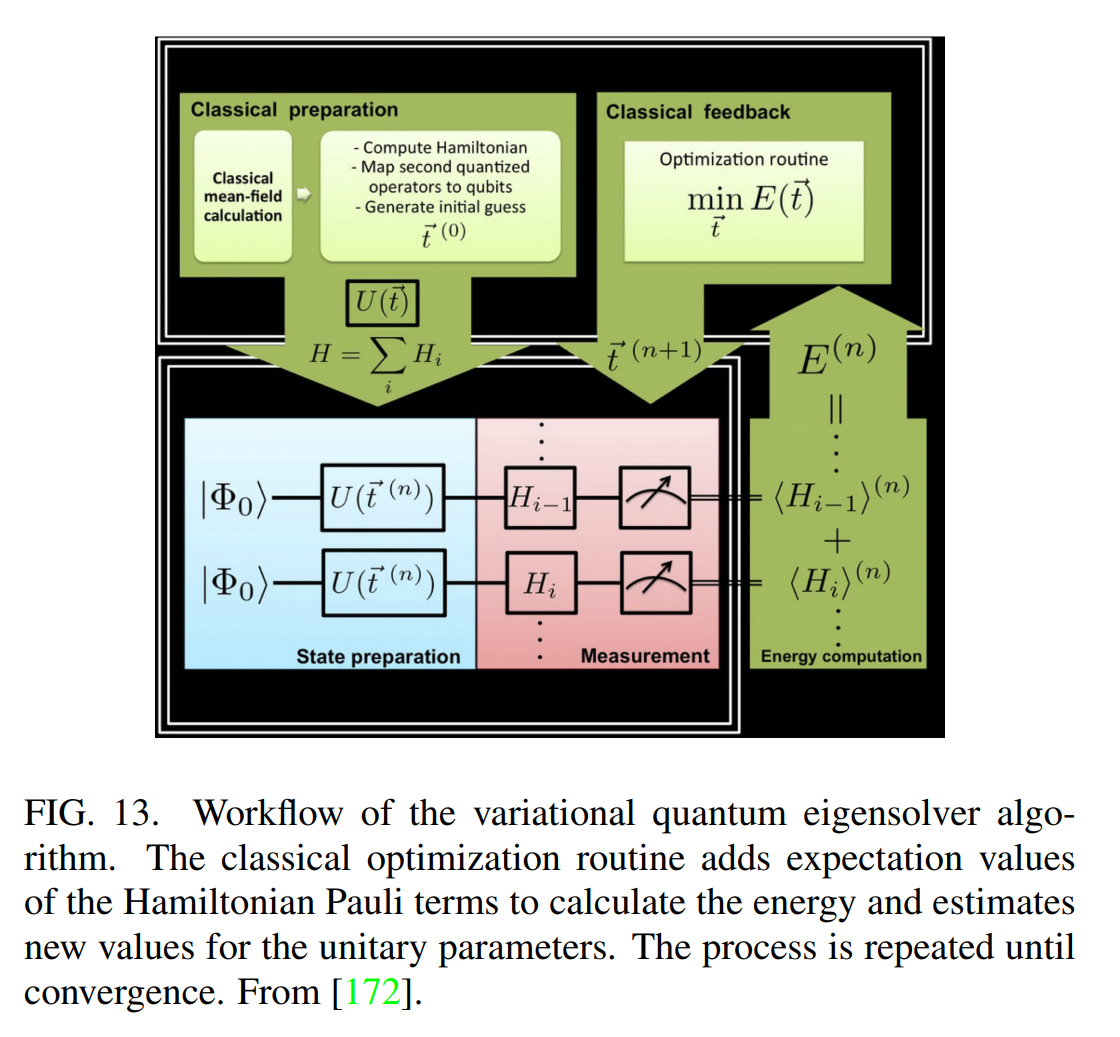
\includegraphics[scale=0.3]{vqei}
	\end{figure}
	We won't worry about the details of how this works at this point. For more information, consider this \href{https://iopscience.iop.org/article/10.1088/2058-9565/aad3e4/pdf}{\underline{paper}}.
	

	
	\item \textit{Adapt-VQE ansatz:}\\
	
	In the adapt-VQE scheme, a collection of operators $\hat{A}_i$ is chosen in advance, and the ground state is approximated by 
	\begin{align}
	\ket{\psi_{\text{adapt-VQE}}} = e^{\theta_n \hat{A}_n}\dots e^{\theta_1 \hat{A}_1}\ket{\psi_{\text{HF}}},
	\end{align}
	Given a current parameter configuration $\vec{\theta}$, the commutator  of the Hamiltonian with each operator in the pool is measured to obtain the gradient of the energy
	\begin{align}
	E = \bra{\psi_{\text{adapt-VQE}}} \had \ket{\psi_{\text{adapt-VQE}}}.
	\end{align}
	wrt the parameters $\vec{\theta}$. Repeating this multiple times and averaging over the obtained samples gives the gradient of the expectation value of the Hamiltonian wrt to the coefficient of each operator. The ansatz is improved by adding the operator $\hat{A}_i$ with the largest gradient to the left end of the ansatz with a new variational parameter, thereby increasing $n$. The operation is repeated until convergence.  
	
	
	
	
	\item \textit{Other considerations:}\\
	
	 There are other considerations with regards to variational methods, but we won't worry about them too much for now.
\end{enumerate}






\subsubsection{Excited states}

While much of the above discussion of state preparation
and variational algorithms has focused on ground-states, most
of the same methods can also be used with minor extensions
for excited states. For example, adiabatic state preparation can
be used to prepare an excited state, so long as it is connected
to the initial state without a vanishing gap.


\subsubsection{Phase estimation}

We have a section on this, so let's just be brief and gloss over the details. \\


Quantum Phase Estimation (QPE) is a crucial step in many
quantum algorithms. QPE enables high-precision measurements of the ground and excited energy levels. This is done by preparing a trial initial state $\ket{\psi(0)}$ that has a non-negligible overlap with the relevant eigenvector of the target Hamiltonian $\had$ and applying a circuit that creates a superposition of time evolved states $\ket{\psi(t)} = e^{-i\had t}\ket{\psi(0)}$ over a suitable range of evolution times $t$. \\

Since QPE is used ubiquitously in a variety of quantum applications, it is crucial to optimize its performance. Below we
list some open problems that are being actively investigated:
\begin{itemize}
	\item Given limitations of near-term quantum devices, of particular interest are tradeoffs between the depth of the
	QPE circuit and its spectral-resolution power as well
	as its sensitivity to noise.
	
	\item Several methods have been proposed for mitigating experimental errors for VQE-type simulations. Such methods enable reliable estimation of expected values of observables on a given trial state without introducing any overhead in terms of extra qubits or quantum gates.
	
	
	\item Classical post-processing methods that enable simultaneous estimation of multiple eigenvalues are highly desirable.
	
	\item Finally, a natural question is whether the time evolution
	operator $e^{-i \had t}$
	in QPE can be replaced by some other
	functions of Hˆ that are easier to implement
\end{itemize}




\subsubsection{Quantum algorithms for time evolution}


\begin{enumerate}
	\item \textit{Hamiltonian simulation problem:}  \\
	
	A quantum computer can be programmed to efficiently simulate the unitary time evolution of almost any physically realistic quantum system. Consider any evolution which is of course given by the SE
	\begin{align}
	i \p_t \ket{\psi(t)} = \had \ket{\psi(t)}, \quad t \geq 0.
	\end{align}
	We can just assume that $\had$ describes a system of $n$ qubits, since any fermionic or spin system can be mapped to qubits. Integrating we get
	\begin{align}
	\ket{\psi(t)} = e^{-i\hat t}\ket{\psi(0)}.
	\end{align}
	A quantum algorithm for Hamiltonian simulation takes as input a description of $\had$, the evolution time $t$, nd outputs a quantum circuit $\U$ that approximates the time evolution operator $e^{-it\had}$ within a specified precision $\epsilon$:
	\begin{align}
	\norm{\U - e^{-it\had}} \leq \epsilon.
	\end{align}
	$\U$ may use ancillary qubits initialized in the $\ket{0}$ state. The simulation cost is usually quantified by the runtime of the algorithm (gate count) and the total number of qubits. Applying $\U$ to $\ket{\psi(0)}$ gives the approximation state $\ket{\psi(t)}$. \\
	
	
	Quantum simulation algorithms apply to general classes of Hamiltonians satisfying mild technical conditions that enable a quantum algorithm to access the Hamiltonian efficiently.

\end{enumerate}

















%\subsubsection{Algorithmic tools}
%\subsubsection{Open problems}
%\subsubsection{Finite-temperature algorithms}
%\subsubsection{Hybrid quantum-classical methods}
%\newpage
%
%
%\subsection{Reading out results}
%
%\subsubsection{Equal-time measurements}
%\subsubsection{Dynamical properties and Green's functions}






\newpage






\section{Quantum Phase Estimation (QPE)}

One of the most important applications of the Quantum Fourier Transform is the Quantum Phase Estimation. Phase estimation is the key for many quantum algorithms. Suppose a unitary operator $\U$ has an eigenvector $\ket{u}$ with eigenvalue $2^{2\pi i \varphi}$, where the value of $\varphi$ is unknown. The goal of the phase estimation algorithm is to estimate $0 \leq \varphi \leq 1$ with high probability within additive error $\epsilon$. The algorithm uses $\mathcal{O}(\log (1/\epsilon))$ qubits and $\mathcal{O}(1/\epsilon)$ controlled-$\U$ operations. \\

To perform the estimation we assume that we have available \textit{oracles} capable of preparing the state $\ket{u}$ (the eigenstate) and performing the controlled-$\U^{2j}$ operation, for suitable nonnegative integers $j$. Since preparing eigenstates is not necessarily easy, the phase estimation algorithm is not a complete algorithm by itself. Rather, we should view it as a ``subroutine'' or a ``module.''\\



The QPE uses two registers. The first register contains $t$ qubits initially in $\ket{0}$. The choice of $t$ depends on two things: the number of digits of accuracy we wish to have in our estimate of $\varphi$, and with what probability we wish the phase estimation procedure to be successful. The second register begins in the eigenstate $\ket{u}$, and contains as many qubits as necessary to store $\ket{u}$. \\

QPE occurs in two main stages. First, the circuit applies  an $\had$ to each of the $t$ qubits. Then, the circuit applies controlled-$\U$ operators on the second register, with $\U$ raised to successive powers of two. This stage looks like the following:
\begin{figure}[!htb]
	\centering
	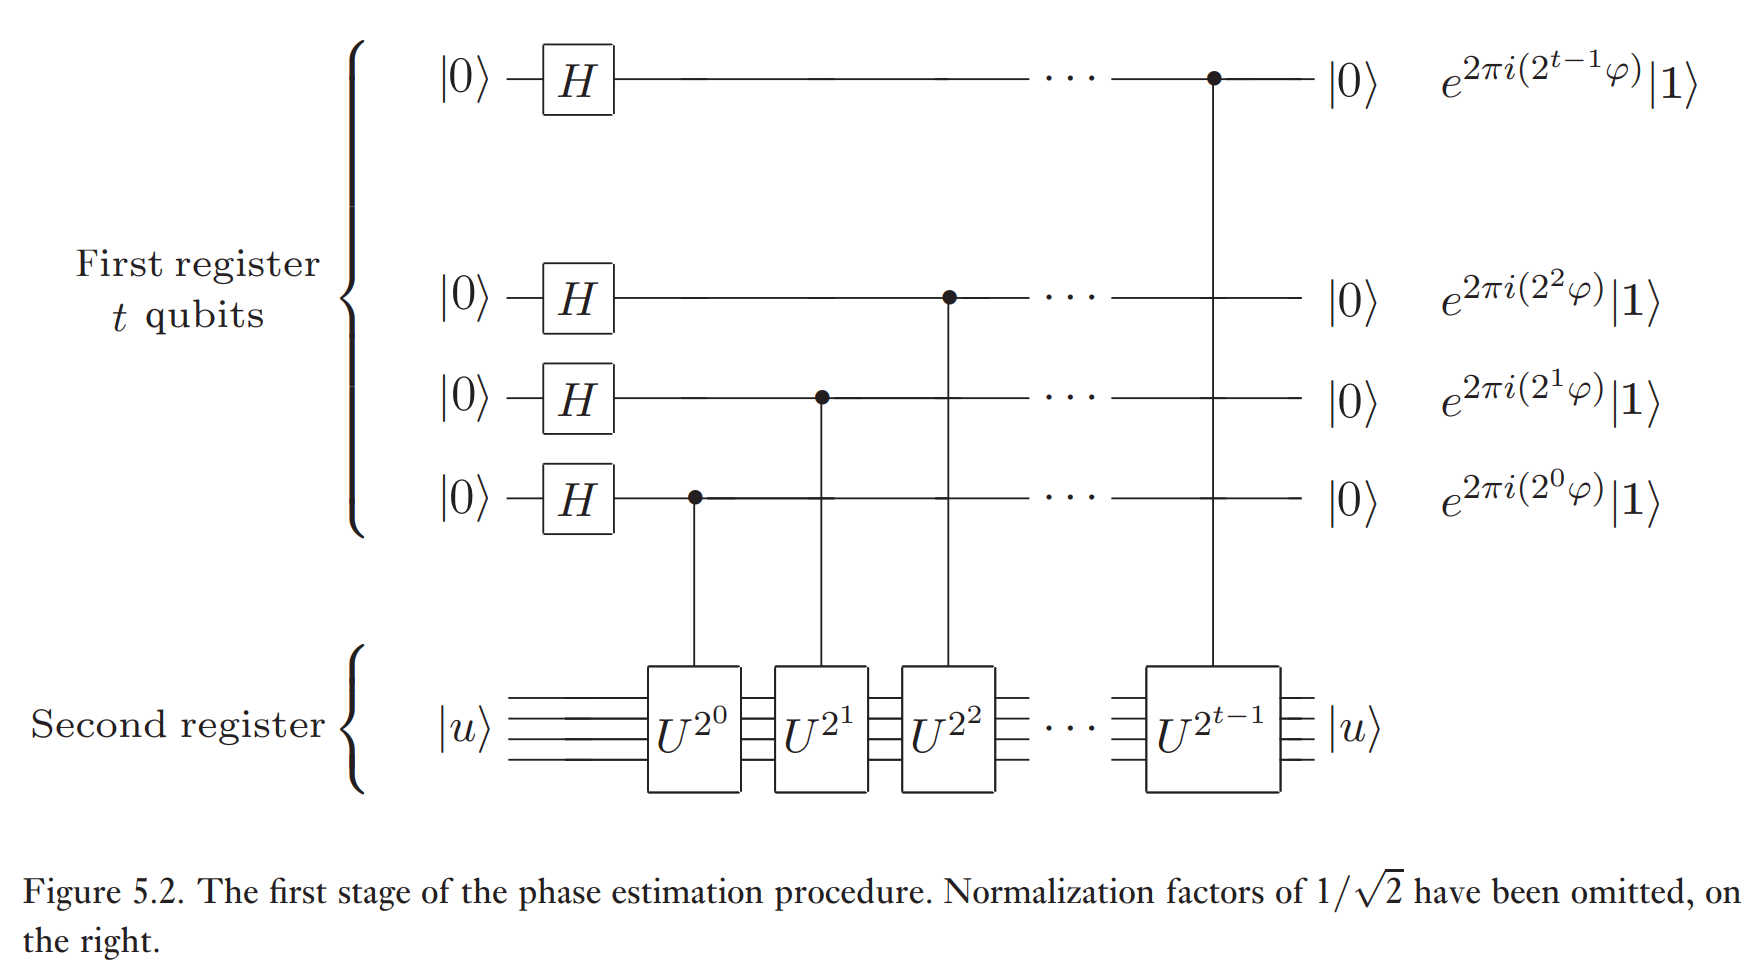
\includegraphics[scale=0.25]{qpe1}
	\caption{Source: Mike and Ike}
\end{figure} 
Recall that immediately after $\had^{\otimes t}$ the state of the upper register looks like
\begin{align}
\had \ket{0} = \f{1}{2^{1/2}}\lp \ket{0} + \ket{1} \rp
\end{align}
The controlled-$\U$ acts on $\ket{u}$ only if the control qubit is in $\ket{1}$. With this, we see that the final state of the first register is given by
\begin{align}
&\f{1}{2^{t/2}}\lp \ket{0} + e^{2\pi i 2^{t-1}\varphi}\ket{1} \rp\otimes
\lp \ket{0} + e^{2\pi i 2^{t-2}\varphi}\ket{1} \rp \otimes \dots \otimes \lp \ket{0} + e^{2\pi i 2^{0}\varphi}\ket{1} \rp\nn\\
&\quad = \dots \nn\\
&\quad = \f{1}{2^{t/2}}\sum_{0\leq k < 2^{t}} e^{2\pi i \varphi k}\ket{k}_t.
\end{align}

\begin{exmp}
For $t =2$, we have
\begin{align}
&\f{1}{2}\lp \ket{0} + e^{4\pi i \varphi } \ket{1} \rp\otimes \lp \ket{0} + e^{2\pi i\varphi }\ket{1} \rp \nn\\
&\quad= \f{1}{2}\lp \ket{0}_2 + e^{1\cdot 2\pi i\varphi }\ket{1}_2 + e^{2\cdot 2\pi i\varphi}\ket{2}_2 + e^{3\cdot 2\pi i\varphi }\ket{3}_2  \rp\nn\\
&\quad = \f{1}{2^{2/2}}\sum_{0 \leq k < 2^{2}}e^{2\pi i \varphi \cdot 2}\ket{k}_2
\end{align}\qed
\end{exmp}

Note that we're leaving out the qubits carrying the  $\ket{u}$ state because we don't do anything to it (because $\ket{u}$ is an eigenstate of $\U$). We should also note that the effect of the sequence of controlled-$\U$ operations is to take $\ket{j}\ket{u}$ to $\ket{j}\U^j \ket{u}$. We should also note that this does not depend on the fact that $\ket{u}$ is an eigenstate of $\U$. \\


In the second state, the algorithm applies the inverse quantum Fourier transform on the first register (which is just the QFT, applied in reverse order of operations). This can be done efficiently in $\mathcal{O}(t^2)$ steps, as we have seen the Quantum Information \href{https://huanqbui.com/LaTeX 20projects/HuanBui_QI/HuanBui_QI.pdf}{\underline{notes}}. Since the input in this case is the maximal superposition in the $t$-vector space, the output of the inverse QFT is going to be a single state: $\ket{\tilde{\varphi}}$, which we hope is approximately $\ket{\varphi}$. We will see how close $\ket{\tilde\varphi}$ can get to $\ket{\varphi}$.\\

The third and final stage of the algorithm is to read out the state of the first register by doing a measurement in the computational basis. \\


\begin{exmp}
	To make sure we see what is going on, suppose $\varphi$ is expressed exactly in $t$ qubits, as $\varphi = 0,\varphi_1\varphi-2\dots\varphi_t$ (note that $\varphi \in [0,1]$). Then the state of the input register after the first stage is given by
	\begin{align}
	\f{1}{2^{t/2}}\lp \ket{0} + e^{2\pi i 0.\varphi_t} \ket{1} \rp \otimes \lp \ket{0} + e^{2\pi i 0.\varphi_{t-1}\varphi_t}\ket{1} \rp \otimes \dots  \otimes \lp \ket{0} + e^{2\pi i 0.\varphi_1\varphi_2\dots\varphi_t}\ket{1} \rp.
	\end{align}
	Applying the inverse QFT to this, we see that output state from the second state is the product state $\ket{\varphi_1\dots \varphi_t}$. A measurement in the computational basis gives $\varphi$ exactly. \qed
\end{exmp}

Schematically, the algorithm for QPE looks like the following:
\begin{figure}[!htb]
	\centering
	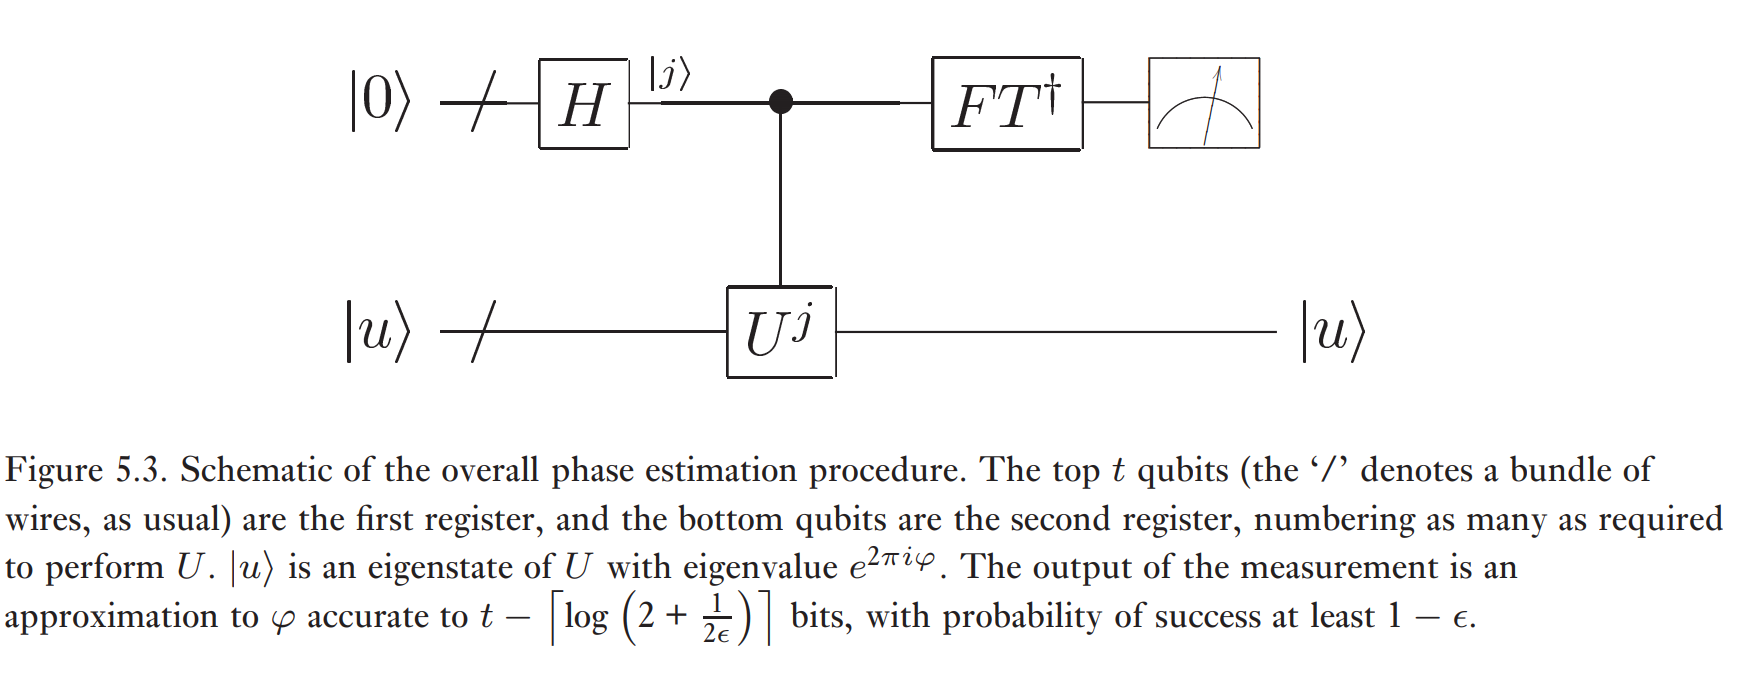
\includegraphics[scale=0.25]{qpe2}
	\caption{Source: Mike and Ike}
\end{figure}

In summary, what we basically did was using the inverse QFT to get
\begin{align}
\f{1}{2^{t/2}}\sum_{0 \leq k < 2^{t}} e^{2\pi i \varphi j }\ket{j}\ket{u} \to \ket{\tilde{\varphi}}\ket{u}
\end{align}
where $\ket{\tilde\varphi}$ is a good estimator for $\varphi$ when measured. 

 





\subsection{Performance and Requirements}
What happens when $\varphi$ cannot be written exactly with a $t$-bit expansion? We will now show that the procedure we described will produce a good approximation to $\varphi$ with high probability. \\

Let $b \in [0,2^t-1]$ an integer be given such that $b/2^t = 0.b_1b_2\dotsb_t$ is the best $t$ bit approximation to $\varphi$ which is less than $\varphi$, i.e., 
\begin{align}
0 \leq \delta \equiv \varphi - b/2^t \leq 2^{-t}.
\end{align}
(This is getting pretty close to an analysis proof -- because it \textit{is} an analysis proof.) Applying the inverse QFT to the state immediately after the first stage gives
\begin{align}
\mathcal{F}^{-1}\lb\f{1}{2^{t/2}}\sum_{0 \leq k < 2^t}e^{2\pi i \varphi k}\ket{k} \rb &= \f{1}{2^{t}} \sum_{0 \leq k,l < 2^t} e^{\f{-2\pi i kl}{2^t}}e^{2\pi i \varphi k}\ket{l}\nn\\
& = \f{1}{2^t}\sum_{0 \leq k,l < 2^t}\lp e^{2\pi i(\varphi- l/2^t)} \rp^k \ket{l}
\end{align}
by definition. Note that when $\varphi$ can be expressed using exactly $t$ bits we are reduced to the simpler version of the problem described above. \\

Let $\al_l$ be the amplitude of $\ket{(b+l) \mod 2^t}$, i.e., 
\begin{align}
\alpha_l \equiv \f{1}{2^t}\sum_{0 \leq k < 2^t} \lp e^{2\pi i (\varphi - (b+l)/2^t)} \rp^k.
\end{align}
This is a partial sum of a geometric series. It is straightforward to show that
\begin{align}
\alpha_l = \f{1}{2^t}\lp \f{1 - e^{2\pi i (2^t \varphi - (b+l))}}{1 - e^{2\pi i (\varphi - (b+l)/2^t)}} \rp = \f{1}{2^t}\lp \f{1 - e^{2\pi i (2^t \delta - l)}}{1 - e^{2\pi i (\delta - l/2^t)}} \rp.
\end{align}
Suppose the outcome of the final measurement is $m$. We want to bound the probability that $\abs{m-b} > \epsilon$ (where $\epsilon$ is the tolerance), i.e., we don't want the probably that $m$ is far from $b$ to be large. Well, the probability of observing such an $m$ is given by
\begin{align}
P(\abs{m-b} > \epsilon) = \sum_{-2^{t-1} < l \leq -(\epsilon+1)} \abs{\al_l}^2 + \sum_{e+1 \leq l \leq 2^{t-1}}\abs{\al_l}^2.
\end{align}
For any real $\theta$, we have $\abs{1 - \exp(i\theta)} \leq 2$, so 
\begin{align}
\abs{\al_l} \leq \f{2}{2^t \abs{1 - e^{2\pi i (\delta - l/2^)}}}.
\end{align}
Further, provided $-\pi \leq \theta \leq \pi$, we have $\abs{1 - \exp(i\theta)} \geq 2\abs{\theta}/\pi$. Also, when $-2^{t-1} < l \leq 2^{t-1}$ we have $-\pi \leq 2\pi (\delta - l/2^t) \leq \pi$, so we have
\begin{align}
\abs{\al_l} \leq \f{1}{2^{t+1}(\delta - l/2^t)}.
\end{align}
With this we have
\begin{align}
p(\abs{m-b} > \epsilon) &\leq \f{1}{4}\lp \sum_{l = -2^{t-1}+1}^{-(\epsilon+1)} \f{1}{(l - 2^t \delta)^2} + \sum^{2^{t-1}}_{l = \epsilon+1} \f{1}{(l - 2^t \delta)^2}  \rp\nn\\
&\leq \f{1}{4}\lp \sum_{l = -2^{t-1}+1}^{-(\epsilon+1)} \f{1}{(l - 1)^2} + \sum^{2^{t-1}}_{l = \epsilon+1} \f{1}{(l - 1)^2}   \rp, \quad 0 \leq 2^t\delta < 1\nn\\
&\leq \f{1}{2}\sum^{2^{t-1}-1}_{l=\epsilon} \f{1}{l^2}\nn\\
&\leq \f{1}{2}\int^{2^{t-1}-1}_{\epsilon-1} \f{1}{l^2}\,dl\nn\\
&= \f{1}{2(\epsilon-1)}.
\end{align}
Suppose we wish to approximate $\varphi$ to an accuracy $2^{-n}$, i.e., we choose $\epsilon = 2^{t-n}-1$. By using $t =n+p$ qubits, we see that the probability of obtaining an approximation correct to this accuracy is at least 
\begin{align}
1-\f{1}{2(\epsilon-1)} = 1 - \f{1}{2(2^p - 2)}.
\end{align}
So, to successfully obtain $\varphi$ accurate to $n$ bits with probability of success at least $1-\epsilon$ we choose 
\begin{align}
t = n + \left\lceil \log \lp 2 + \f{1}{2\epsilon} \rp \right\rceil.
\end{align}

Now here's a catch: to use QPE, we need the eigenstate $\ket{u}$. What if we don't know how to prepare such a state? Suppose that we prepare some other state $\ket{\psi}$ in place of $\ket{u}$. We can write
\begin{align}
\ket{\psi} = \sum_u c_u \ket{u}
\end{align}
where $\ket{u}$ are the eigenstates of $U$. Suppose the eigenstate $\ket{u}$ has the eigenvalue $e^{2\pi i \varphi_u}$. Running the QPE on $\ket{\psi}$ will give
\begin{align}
\ket{\psi} \stackrel{\mbox{QPE}}{\to} \sum_u c_u \ket{\tilde{\varphi_u}}\ket{u},
\end{align}
where $\tilde{\varphi_u}$ is an estimation for $\varphi_u$. Reading out the first register gives us a good approximation for $\varphi_u$, where $u$ is chosen at random with probability $\abs{c_n}^2$. This procedure allows us to avoid preparing a possibly unknown eigenstate, but at the cost of introducing some additional randomness into the algorithm. It turns out that if $t$ is chosen according to the minimization procedure above, then the probability for measuring $\varphi_u$ accurate to $n$ bits at the conclusion of the phase estimation algorithm is at least $\abs{c_u}^2(1-\epsilon)$.







\subsection{The algorithm}
QPE solves a problem which is both non-trivial and interesting from a physical point of view. It allows us to estimate the eigenvalue associated to a given eigenvector of a unitary operator. It turns our that other interesting problems can be reduced to phase estimation, which makes QPE particularly useful.\\

\underline{Here's the algorithm:}
\begin{itemize}
	\item \textbf{Inputs:} (1) An oracle which performs a controlled-$\U^j$ operation, (2) an eigenstate $\ket{u}$ of $\U$ with eigenvalue $e^{2\pi i \varphi_u}$, and (3) $t = n + \left\lceil \log \lp 2 + 1/2\epsilon \rp \right \rceil$ qubits initialized to $\ket{0}$.
	
	
	\item \textbf{Outputs:} An $n$-bit approximation $\tilde\varphi_u$ of $\varphi_u$. 
	
	\item \textbf{Runtime:} $\mathcal{O}(t^2)$ operations (due to th inverse QFT) and one call to controlled-$\U^j$ oracle. Succeeds with probability at least $1-\epsilon$. 
	
	\item \textbf{Procedure:} 
	\begin{itemize}
		\item  Initial state: $\ket{0}\ket{u}$
		
		\item Create superposition: $\to (1/2^{t/2})\sum_{0 \leq j < 2^t}\ket{j}\ket{u}$.
		
		
		\item Apply the oracle:\\ $\to(1/2^{t/2})\sum_{0 \leq j < 2^t}\ket{j}\U^j\ket{u} = (1/2^{t/2})\sum_{0 \leq j < 2^t}e^{2\pi i j\varphi_u}\ket{j}\ket{u}$
		
		
		\item Apply inverse QFT: $\to \ket{\tilde\varphi_u}\ket{u}$. 
		
		\item Measure the first register: $\to \tilde \varphi_u$.
	\end{itemize}
\end{itemize}


The algorithm has a wide range of applications, including order-finding and factorization. 










\newpage


\section{Quantum Variational Eigensolver (QVE)}      

In this section we're looking this \href{https://www.ncbi.nlm.nih.gov/pmc/articles/PMC4124861/pdf/ncomms5213.pdf}{\underline{paper}} on the quantum variational eigensolver (QVE). \\


For quantum systems, where the physical dimension grows exponentially, finding the eigenvalues of certain operators is one of many intractable problem and remains a fundamental challenge.  QPE efficiently finds the eigenvalue of a given eigenvector but requires fully coherent evolution. This paper presents an alternative approach that greatly reduces the requirements for coherent evolution and combine this method with a new approach to state preparation based on ansatz and classical optimization. \\

As we have seen, quantum approaches to finding eigenvalues
have previously relied on the quantum phase estimation (QPE)
algorithm. The QPE algorithm offers an exponential speedup
over classical methods and requires a number of quantum operations $\mathcal{O}(p^{-1})$ to obtain an estimate with precision $p$. Recall that in the standard formulation of QPE, one assumes the eigenvector $\ket{\psi}$ of a Hermitian operator $\had$ is given as input and the problem is to determine the corresponding eigenvalue $\lambda$. The time the
quantum computer must remain coherent is determined by the
necessity of $\mathcal{O}(p^{-1})$ successive applications of $e^{-i \had t}$, each of which can require on the order of millions or billions of quantum gates for practical applications, as compared to the tens to hndreds og gates achievable in the short term. \\

This paper presents an alternative to QPE that significantly reduces the requirements for coherent evolution. This alternative method is given by a quantum processing unit which efficiently calculates the expectation value of a Hamiltonian, providing an exponential speedup over exact diagonalization, the only known exact solution to the poblem on a traditional computer. In conjunction with a classical optimization algorithm, this approach reduces the requirement for coherent evolution of the quantum state, making more efficient use of quantum resources, and may offer an alternative route to practical quantum-enhanced computation. 





\subsection{Quantum Expectation Estimation (QEE)}


QEE computes the expectation value of a given Hamiltonian $\had$ for an input state $\ket{\psi}$. This is done via the decomposition:
\begin{align}
\had = \sum_{i\alpha}h^i_\alpha \sigma^i_\alpha + \sum_{ij\al\be}h^{ij}_{\al\be}\sigma^i_\alpha \sigma^j_\be + \dots
\end{align}
for real $h$, where Roman indices identify the subsystem on which the operator acts, and Greek indices identify the Pauli operator. For example, $\alpha = x$. This is possible because \textit{products of Pauli matrices form a basis for the set of Hermitian matrices of dimensions that are powers of 2}. In more generality, this is possible because we have the \textit{Pauli group} $G_n$, which is the group generated by the operators applied to each of $n$ qubits in th tensor product Hilbert space $(\mathbb{C}^2)^{\otimes n}$. \\

In any case, I digress. By linearity, we have
\begin{align}
\langle \had \rangle = \sum_{i\al} h^i_\al \langle \sigma^i_\al \rangle + \sum_{ij\al\be} h^{ij}_{\al\be} \langle \sigma^i_\al \sigma^j_\be  + \dot \rangle 
\end{align}
Just as in QPE, we only consider Hamiltonians that can be written as a  polynomial number of terms, wrt the system size. This class of Hamiltonians encompasses a wide range of physical system, so this requirement is not too strict. In fact, Hamiltonians of this kind include the electronic structure Hamiltonian of quantum chemistry, the quantum Ising Model, the Heisenberg Model, matrices that are well approximate as a sum of $n$-fold tensor products, and more generally any $k$-sparse Hamiltonian without evident tensor product structure.\\

\textbf{Remark:} Sparse Hamiltonians are important because it is possible to decompose $\had$ into $\sum_k \had_k$ where $\had_k$'s all commute (making diagonalization straightforward). If the matrix is sparse, then we shouldn't need too many distinct $\had_k$'s. Then we can simulate the Hamiltonian evolution 
\begin{align}
e^{-i\had t} = \prod e^{-i \had_m \delta t}
\end{align}
where $t =N \delta t$. Now, what do we mean by ``sparse?'' Sparse means that there are at most $d$ nonzero entries per row, $d = \text{poly}(\log N)$. In any given row, the location of the $j$th nonzero entry and its value can be compute efficiently (or is given by a black box). Sparse Hamiltonians are different from ``Local'' Hamiltonians, where $\had = \sum_j \had_j$ where each $\had_j$ acts on $\mathcal{O}(1)$ qubits. \qed\\



In any case, I digress again. The evaluation of $\langle \had \rangle $ reduces to the sum of a polynomial number of expectation values of simple Pauli operators for a quantum state $\ket{\psi}$,  multiplied by some real constants. A quantum device can efficiently evaluate the expectation value of a tensor product of arbitrary number of simple Pauli operators. Therefore, with an $n$-qubit state we can efficient evaluate the expectation value of this $2^n \times 2^n$ Hamiltonian.\\

This is possible with a classical computer, but it suffers from the $N$-representability problem. The power of the quantum approach derives from the fact that quantum hardware can store a global quantum state with exponentially fewer resources than required by classical hardware, and as a result the $N$-representability problem does not arise. \\


The expectation value of a tensor product of an arbitrary
number of Pauli operators can be estimated by local measurement of each qubit (this can be found somewhere in Mike and Ike). Such independent measurements can be performed in parallel, incurring a constant cost in time. Furthermore, since these operators are normalized an finite-dimensional, their spectra are bounded. As a result, each
\begin{align}
\langle H^m_i\rangle = h^{ij\dots}_{\al\be\dots} \langle \sigma^i_\al \otimes \sigma^i_\be \otimes \dots \rangle  
\end{align}
can be estimated to a precision $p$ of an individual element with coefficient $h$, which is an arbitrary element from the set of constants $\{ h^{ij\dots}_{\al\be\dots}\}$ at a cost of $\mathcal{O}(\abs{h_\text{max}}^2 Mp^{-2})$ repetitions. $M$ is the number of terms in the decomposition of the Hamiltonian and $h_\text{max}$ is the coefficient with maximum norm in the decomposition of the Hamiltonian. \\


The advantage of this approach is that the coherence time to make a single measurement after preparing
the state is $\mathcal{O}(1)$. Conversely, the disadvantage of this approach with respect to QPE is the scaling in the total number of
operations, as a function of the desired precision is quadratically
worse $\mathcal{O}(p^{-2})$ versus $\mathcal{O}(p^{-1})$.  Moreover, this scaling will also reflect the number of state preparation repetitions required, whereas in QPE the number of state preparation steps is constant. In essence, we dramatically reduce the coherence time requirement while maintaining an exponential advantage over
the classical case, by adding a polynomial number of repetitions
with respect to QPE.


\newpage


\subsection{Quantum Variational Eigensolver (QVE)}

The procedure outlined above
replaces the long coherent evolution required by QPE by many
short coherent evolutions. In both QPE and QEE we require a
good approximation to the ground-state wavefunction to compute the ground-state eigenvalue, and we now consider this
problem. The quantum variational eigensolver (QVE) algorithm
is a variational method to prepare the eigenstate and, by
exploiting QEE, requires short coherent evolution. 

\begin{figure}[!htb]
	\centering
	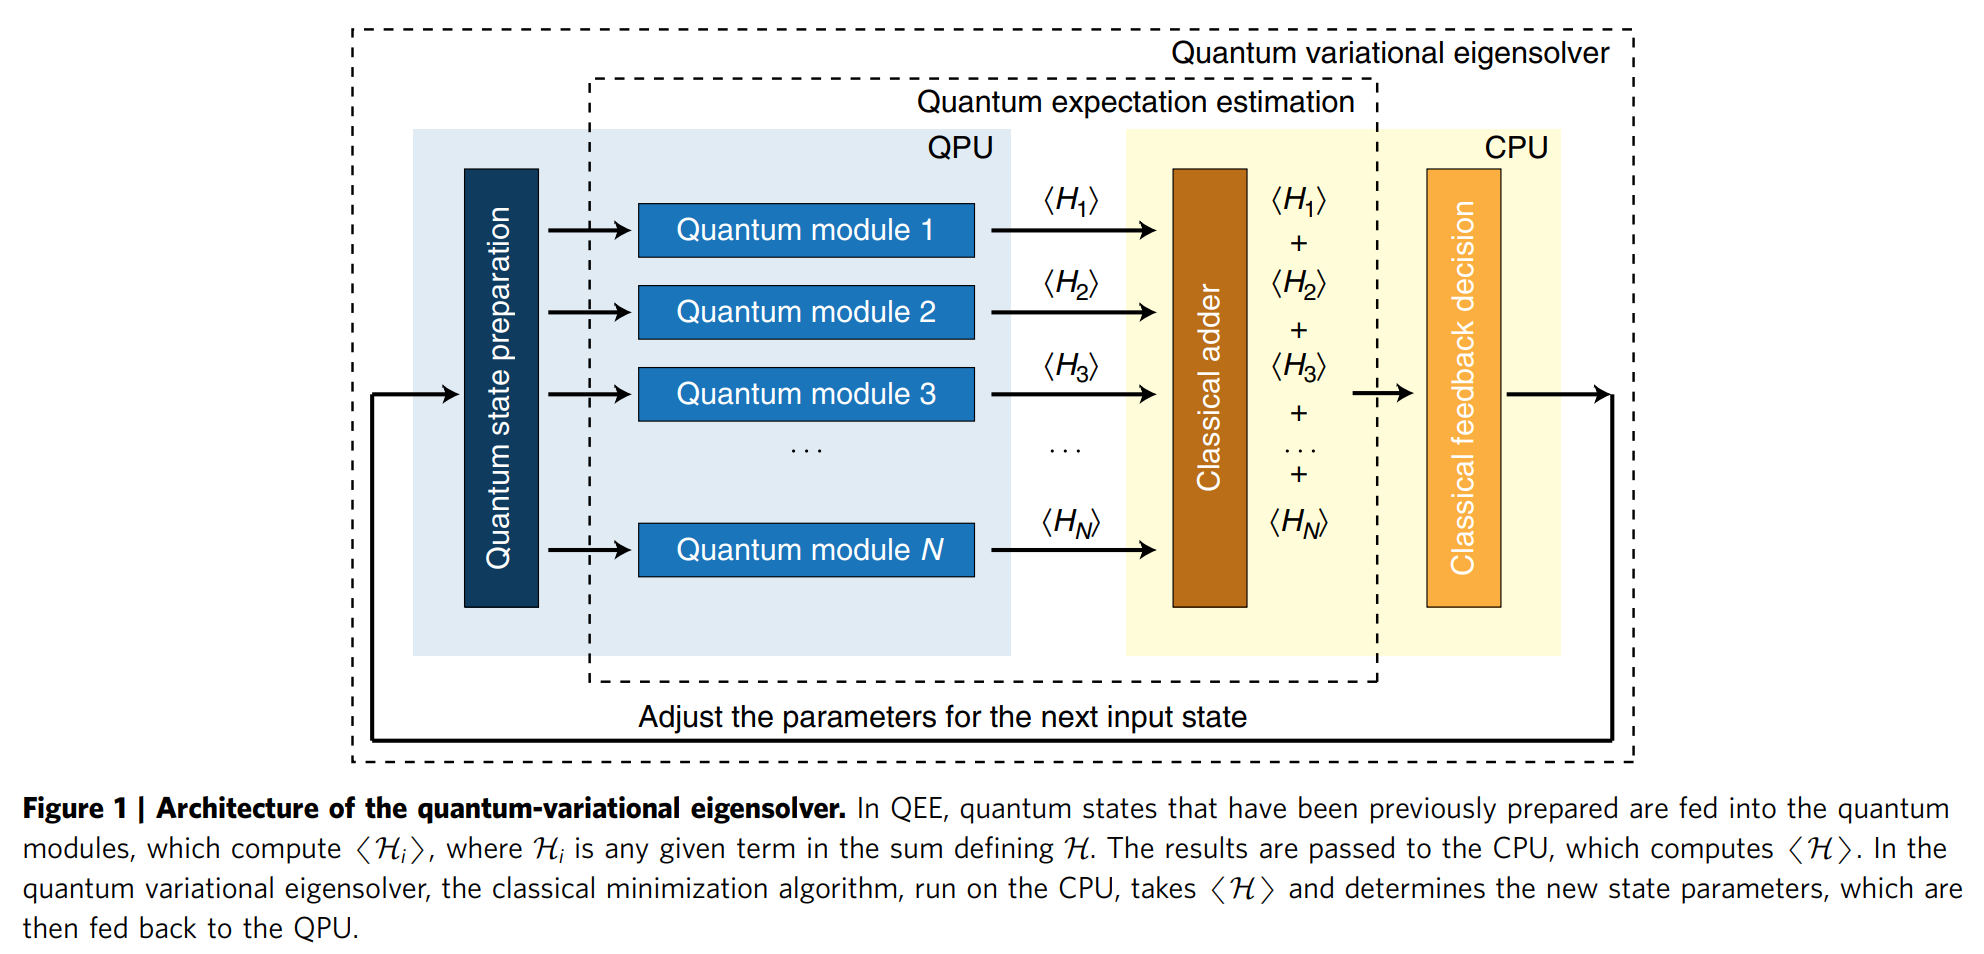
\includegraphics[scale=0.2]{qvei}
\end{figure}

It is well known that the eigenvalue problem for an observable
represented by an operator H can be restated as a variational
problem on the Rayleigh–Ritz quotient such that the eigenvector $\ket{\psi}$ corresponding to the lowest eigenvalue is the one hat minimizes
\begin{align}
\f{\bra{\psi} \had \ket{\psi}}{\braket{\psi}}
\end{align}
By varying the experimental parameters in the preparation of $\ket{\psi}$ and computing the Rayleigh–Ritz quotient using QEE as
a subroutine in a classical minimization, one may prepare
unknown eigenvectors. At the termination of the algorithm, a
simple prescription for the reconstruction of the eigenvector is
stored in the final set of experimental parameters that define $\ket{\psi}$. \\

Note that if a quantum state is characterized by an exponentially large
number of parameters, it cannot be prepared with a polynomial
number of operations. The set of efficiently preparable states are
therefore characterized by polynomially many parameters, and
we choose a particular set of ansatz states of this type.  Under
these conditions, a classical search algorithm on the experimental
parameters that define $\ket{\psi}$ needs only explore a polynomial
number of dimensions -- requirement for the search to be
efficient.\\

One example of a quantum state parameterized by a
polynomial number of parameters for which there is no known
efficient classical implementation is the unitary coupled cluster
ansatz
\begin{align}
\ket{\Psi} = e^{T - T^\dagger}\ket{\Phi}_\text{ref}
\end{align}
where $\ket{\Phi}_\text{ref}$ is some reference state, usually the Hartree Fock ground state, and $T$ is the cluster operator for an $N$ electron system, defined by
\begin{align}
T =T_1 + T_2 + \dots + T_N,
\end{align}
where
\begin{align}
T_1 = \sum_{pr}t^r_p \hat{a}_p^\dagger\hat{a}_r, \quad T_2 = \sum_{pqrs}t^{rs}_{pq}\hat{a}_p^\dagger \hat{a}_q^\dagger\hat{a}_r \hat{a}_s,\quad \dots
\end{align}
By construction, $(T - T^\dagger)$ is anti-Hermitian, and exponentiation maps it to a unitary operator $e^{(T - T^\dagger)}$. \\

For any fixed excitation level $k$, the reduced cluster operator is written as
\begin{align}
T^{(k)} = \sum^k_{i=1}T_i.
\end{align}
This state may be prepared efficiently on a quantum
device. The reduced anti-hermitian cluster operator  $(T^{(k)} - T^{(k)\dagger})$ is the sum of a polynomial number of terms—namely, it contains
a number of terms $\mathcal{O}(N^k(M-N)^k)$, where $M$ is the number of
single-particle orbitals. By defining an effective Hermitian
Hamiltonian $\had = i(T^{(k)} - T^{(k)\dagger})$ and performing the Jordan–
Wigner transformation to reach a Hamiltonian that acts on the
space of qubits $\hat{\had}$, we are left with a Hamiltonian that is a sum of polynomially many products of Pauli operators. The problem then reduces to the quantum simulation of this effective Hamiltonian, $\hat{\had}$ which can be one in polynomial time using known procedures. 





















\newpage




\section{Some Models in Quantum Statistical \& Condensed-Matter Physics}

In this section we will be looking at some of the most well-known and most studied models in statistical and quantum many-body mechanics. I'll be sourcing the material from various places, so I'll try my best to cite all the sources. 


\subsection{The Ising Model}
In this section we'll look at the Ising model from the mathematical physics perspective. I'll try to add connections to physics to the best of my ability. \\

Anyway, the Ising model is the simplest and most famous spin system model to study phase transition. It was introduced in 1925 by Ernst Ising in his PhD thesis. He completely solved the model in one dimension, but mistakenly inferred behaviors in higher dimensions. \\

\subsubsection{Basic definitions}

Let a graph $G = (V,E)$ be given, with state space $\Omega = \{ -1,+1 \}^V$ and elements $\sigma = \{ \sigma_x \}_{x\in V}$. The variable $\sigma_x \in \{ -1,+1\}$ is called the spin at vertex $x$. This is thus a spin system. Under some re-definitions we can think of this as a lattice gas model, but let's not worry about that. \\

The energy functional, or the Hamiltonian, of the system is given by
\begin{align}
\had(\sigma) = -J \sum_{(x,y)\in E} \sigma_x \sigma_y
\end{align}
where $J$ is a real constant, called the interaction strength. In this formulation, $\had$ is built up from the local energy terms $-J \sigma_x \sigma_y$, i.e., the model is defined in terms of nearest-neighbor interactions. Next, we introduce the inverse temperature parameter $\beta \sim 1/T$ and consider the probability measure on $\Omega$:
\begin{align}
\mu(\sigma) = \f{e^{-\beta \had(\sigma)}}{\sum_{\sigma \in \Omega} e^{-\beta\had}} \equiv \f{e^{-\beta \had(\sigma)}}{Z_\beta}
\end{align}
where of course $\Z_\beta$ is called the partition function, which contains all information about the system. $\mu = \mu_\beta$ is called the Gibbs measure. \\

When $J> 0$, we have the ferromagnetic case in which the minimum of $\had(\sigma)$ and so the maximum of $\mu(\sigma)$ are attained at $\sigma \equiv \text{const}$. More generally, spins like to agree along edges, and for $\beta \to \infty$ the measure concentrates on the two constant configurations.s \\

When $J < 0$, we have antiferromagnetism where neighboring spins like to differ. This case is hard, and we're not going to worry about it. \\

For any function $f: \Omega \to \mathbb{R}$, we have the expectation and variance:
\begin{align}
\mu(f) = \langle f \rangle = \sum_{\sigma\in \Omega} \mu(\sigma) f(\sigma), \quad \text{Var}(f) = \mu[f^2] - \mu[f]^2.
\end{align}
So in our case, ``$\mu$'' is like $E[\cdot]$, denoting the expectation value. 


\subsubsection{Thermodynamic objects}

Recall the following definitions
\begin{defn}[Free Energy]
	The free energy of a system with inverse temperature $\beta$ and partition function $Z_\beta$ is given by
	\begin{align}
	F(\beta) = -\f{1}{\beta}\log Z_\beta.
	\end{align}
\end{defn}

We note that 
\begin{align}
Z_\beta = e^{-\beta F(\beta)}
\end{align}
and
\begin{align}
\p_\beta F(\beta) = \mu(\had) = \langle \had \rangle.
\end{align}

\begin{defn}[Specific Heat]
	\begin{align}
	C(\beta) = \f{d}{d(1/\beta)} \mu(\had) = -\beta^2 \f{d}{d\beta^2}F(\beta).
	\end{align}
\end{defn}
We can show that the specific heat is related to the fluctuation of the system via
\begin{align}
C(\beta) = \beta^2 \text{Var}(\had).
\end{align}



Next we modify the Hamiltonian by introducing an external magnetic field:
\begin{align}
\had(\sigma, h) = -J \sum_{(x,y)\in E} \sigma_x \sigma_y - \sum \sum_{x\in V} h_x \sigma_x.
\end{align}
Here $h_x$ are real numbers and sometimes $h_x$ is identically constant. If $h> 0$, $\had$ has a unique minimum at $\sigma = +1$. A very difficult famous problem is the case when the $h_x$'s are iid r.v. \\

Now, 
\begin{align}
F(\beta,h) = -\f{1}{\beta} \log Z(\beta,h).
\end{align}
This is a nice smooth function for any finite graph $G$. With this we consider the magnetization. 

\begin{defn}[Magnetization]
	\begin{align}
	M(\beta, h) = \f{1}{\abs{V}} \sum_{x\in V}\mu(\sigma_x) = -\f{1}{\abs{V}} \p_h F(\beta,h).
	\end{align}
\end{defn}



Both the magnetization and energy will grow as $\abs{V}$ as $V$ grows to infinity, and we would like to take the limit $L\to \infty$ of quantities like magnetization or any expectation value $\langle f(\sigma) \rangle_L$ where $f$ is any function of finitely many spins. These limits are called the ``thermodynamic limit.'' \\

Another quantity of physical interest is the correlation strength. A natural question is how much the spins $\sigma_i$ and $\sigma_j$ at two sites are correlated, especially if the spins are far apart. The simplest measurement of this is
\begin{align}
\langle \sigma_i \sigma_j \rangle - \la \sigma_i \ra \la \sigma_j \ra. 
\end{align}
This quantity is zero if the spins are independent. What typically happens is that this quantity \textbf{decays} exponentially as $\abs{i-j}\to \infty$ for all values of $\beta$ but one. So, 
\begin{align}
\la \sigma_i \sigma_j \ra \equiv \langle \sigma_i \sigma_j \rangle - \la \sigma_i \ra \la \sigma_j \ra \sim e^{-\abs{i-j}/\xi}
\end{align}
as $\abs{i-j}\to \infty$ where $\xi$ is a length scale which is called the \textbf{correlation length}. The correlation length is to some extent a measure of how interesting the system is. A short correlation length means that distant spins are very weakly correlated.\\

Now if there is an external magnetic field then the Hamiltonian becomes
\begin{align}
\had = -\sum_{\la i,j \ra} \sigma_i \sigma_j - h\sum_i \sigma_i 
\end{align}
where $h$ is the magnetic field external parameter. The free energy is defined by
\begin{align}
\exp\lb -\beta F \rb = \mathcal{Z} = \sum_\sigma \exp\lb -\beta \had \rb
\end{align}
where $F$ is a function of the two parameters $\beta$ and $h$ and the choice of the finite volume (so that the Hamiltonian makes sense). The free energy per site $f$ is then given by $F$ divided by the number of sites. Then the magnetization is given by
\begin{align}
m = -\p_h f
\end{align}




When we defined th magnetization before there was no magnetic field term in $\had$. To obtain this magnetization we should set $h=0$ after taking the derivative. However, we can talk about the magnetization of the system with an external field present, $h\neq 0$. The magnetization is then a function of $\beta,h$. The derivative of the magnetization wrt $h$ is called th magnetic susceptibility:
\begin{align}
\chi = \p_h m = -\p^2_h f.
\end{align}
By taking the derivative of $\beta f$ wrt $\beta$ one obtains the energy per site. The second derivative of $f$ wrt $\beta$ is known as the specific heat and denoted
\begin{align}
C = \p_\beta^2 f.
\end{align}


\subsubsection{Phase transition - the role of the boundary conditions}

We will start by asking whether the boundary conditions make a difference in the infinite volume limit. In a finite volume we might guess that $+$ boundary conditions would make the spin at the origin a little more likely to be $+1$ than $-1$. What happens when $L \to \infty$? It turns out that the answer depends on $\beta$. \\

In this section, I will just list some theorems/lemmas without showing proofs. We will just focus on the results for now. 

\begin{thm}
	If the number of dimensions is at least two, then there is a positive number $\beta_c$ such that for $\beta < \beta_c$ the limit $\lim_{L\to \infty} \la \sigma_0 \ra_L^+$ exists and is zero while for $\beta > \beta_c$ the limit exists and is strictly greater than zero. 
\end{thm}

The notation $\la \cdot \ra^+$ denotes the positive boundary condition. This just means that all of the outside spins are $+1$ initially. The intuition is that when $\beta$ is small, the spins should only be weakly correlated. The influence of the boundary condition will decay rapidly as we move in from the boundary. 



\begin{thm}
	In any number of dimensions there is a positive number $\beta_1$ such that for $\beta < \beta_1$ the limits $\lim_{L\to \infty}\la \sigma_o \ra^+_L$ and $\lim_{L\to \infty} \la \sigma_0 \ra^-_L$ are both zero. 
\end{thm}




\begin{thm}
	In two or more dimensions there is a positive number $\beta_2$ such that for $\beta > \beta_2$ the limit $\lim \inf_{L\to \infty} \la \sigma_0 \ra^+_L$ s strictly greater than zero for $+$ boundary conditions. 
\end{thm}


\subsubsection{Phase transitions and critical phenomena}


Crudely speaking a phase transition is when an abrupt change occurs in the infinite volume system at some values of the parameters like temperature and magnetic field. Th values of the parameters where this happens are called a \textit{critical point}. \\

What typically happens is that when $T \to T_c$ some physical quantities diverge while other converge to zero. The way in which they do so, though, is interesting. Correlation length goes to zero as $T\to \infty$ and $T\to 0$. At $T_c$, the correlation length goes to $\infty$. We can think of phase transition as the correlation length diverging. \\

As $T\to T_c$ the specific heat  and magnetic susceptibility also diverge to $\infty$. As $T\to T_c^-$ the magnetization $m$ will converge to zero. 





































\subsection{The Hubbard Model}

In this section we will look at this \href{https://www.cond-mat.de/events/correl16/manuscripts/scalettar.pdf}{\underline{document}} on the Hubbard Hamiltonian. In some sense the HH is quite similar to the Ising model, except that it is written in terms of fermionic creation and annihilation operators. \\

I'm not sure we have time to cover this partially (or even at all!), but here's the layout: 
\begin{itemize}
	\item Introduction
	\item Creation and Annihilation operators
	\item The Hubbard Hamiltonian
	\item Particle-hole symmetry
	\item The single-site limit
	\item The non-interacting Hubbard Hamiltonian
	\item Exact diagonalization: two-site HH
	\item Green functions: Mott gap and spectral function
	\item A peek at magnetism
	\item $\dots$
	\item Conclusions
\end{itemize}















\newpage




\section{Locality in Quantum Systems}

In this section we will look at this \href{https://arxiv.org/pdf/1008.5137.pdf}{\underline{paper}} by Matthew Hastings. This is actually a compilation of lecture notes focusing on the application of ideas of locality, in particular Lieb-Robinson bounds, to quantum many-body systems. For our purposes, we will only look at a few topics included. 
\begin{itemize}
	\item We want to understand ``locality'' in the context of quantum simulation. What, precisely, does it mean for a Hamiltonian to be ''local''? 
	
	\item What are the Lieb-Robinson bounds? 
	
	\item What is the Lieb-Schulz-Mattis theorem?
	
	\item What are topologically ordered states? 
\end{itemize}





\subsection{Introduction \& Notation}

The basic problem studied in quantum many-body theory is to find the properties of the ground state of a given
Hamiltonian. Expressed mathematically, the Hamiltonian $\had$ is a Hermitian matrix, and the ground state, which we write $\psi_0$, is an eigenvector of this matrix with the lowest eigenvalue.  The properties we are interested in studying
are expectation values of various observables: given a Hermitian matrix $O$, we would like to compute the expectation value $\langle \psi_0 , O \psi_0\rangle \equiv \langle O \rangle$. \\

While the method of ``exact diagonalization'' on a computer is an important technique in studying
quantum systems, it is only a small part of how physical problems are studied. The feature that distinguishes the study of quantum many-body systems is \textit{locality} of interactions. Consider a typical Hamiltonian, such as the one-dimensional transverse field Ising model TFIM):
\begin{align}
\had = -J \sum^{N-1}_{i=1}S^z_i S^z_{i+1} + B \sum^{N}_{i=1}S_i^x.
\end{align}
The very notation implicitly assumes local interactions. To be precise, throughout this section, we only consider quantum systems on a finite size lattice. We associate a $D$ dimensional Hilbert space with each lattice site, and the Hilbert space of the whole system is tensor product of these spaces. We use $N$ to represent the number of lattice sites, so that the Hilbert space on which a Hamiltonian such as the one above is defined in $D^N$ dimensions. A term such as $S^z_i S^z_{i+1}$ is short hand for $I_1 \otimes I_2 \otimes \dots \otimes S_i^z \otimes S^z_{i+1} \otimes I_{i+2} \otimes \dots \otimes I_N$, where $I_j$ is the identity operator on site $j$.\\

We let $i,j,k,\dots$ denote the lattice site, and $X,Y,Z$ to denote sets of lattice sites. We se $\Lambda$ to denote the set of all lattice sites. We use $\abs{X}$ to denote the cardinality of a set $X$. \\

An operator $O$ is supported on a set $A$ if we can write $O$ as a tensor product of two operators $O = I_{\Lambda\setminus A} \otimes P$, where $I_{\Lambda \setminus A}$ is the identity operator on the sites not in $A$ and $P$ is some operator defined on the $D^{\abs{A}}$ dimensional Hilbert space on the set $A$. For example, $S^z_i \otimes S^z_{i+1}$ is supported on the set $\{ i, i+1\}$. \\

We let $\norm{O}$ denote the ``operator norm'' for $O$. If $O$ is Hermitian, the operator norm is the equal to the absolute value of the largest eigenvalue of $O$. For arbitrary operators $O$, the operator norm is given by
\begin{align}
\norm{O} = \max_{\psi, \abs{\psi} = 1}  \abs{O \psi},
\end{align}
which one might have seen in real/functional analysis. \\

Using 2 simple assumptions: that the Hamiltonian has local interactions and that the Hamiltonian has a spectral gap, we will be able to prove a wide variety of results about the ground state of the Hamiltonian. We will consider two cases of a spectral gap: one where $E_1  - E_0 \geq \Delta E$, where $\Delta E$ is called the ``spectral gap.'' In the other case, we consider a Hamiltonian with several degenerate or approximately degenerate low energy states. \\

We will begin by considering properties of correlations in these systems, and prove an exponential decay of correlation functions. We then consider how the ground state of the system changes under a change in the Hamiltonian, and use this to prove a non-relativistic variant of Goldstone's Theorem. Finally, we apply these techniques to more interesting systems with topological order, beginning with the Lieb-Schultz-Mattis theorem However, before we can do any of this, we need to more precisely define the locality properties of the Hamiltonian and to prove a set of bounds on te propagation of information through the system called the Lieb-Robinson bounds. 



\subsection{Locality \& The Lieb-Robinson bounds}


To define locality, we need a notion of distance, so we introduce a metric on the lattice $d(i,j)$. One may consider the Manhattan or Euclidean metric. It's natural to consider the metric 
\begin{align}
d(i,j) = \min_n \abs{i-j + nN}
\end{align}
for a one-dimensional system with periodic boundary conditions and $N$ sites. Next, we define the distance between two sets $A,B$ to be
\begin{align}
d(A,B) = \min_{a\in A, b\in B}d(a,b).
\end{align}
The diameter of a set $A$ is given by
\begin{align}
\text{diam}(A) = \max_{i,j\in A}d(i,j).
\end{align}
Next we consider Hamiltonians
\begin{align}
\had = \sum_Z H_Z
\end{align}
where each $H_Z$ is support on $Z$. We are interested in studying problems in which $\abs{H_Z}$ decays rapidly with $\text{diam}(Z)$. \\


(\textit{to be continued})





\newpage


\section{Quantum Approximate Optimization Algorithm (QAOA)}

\textit{Let's not worry about this now.}


\newpage

\section{Quantum Variational Factorization (QVF)}

\textit{Let's not worry about this now.}

\newpage



\section{Variational Thermal Quantum Simulation via Thermofield Double States}

\textit{Let's not worry about this now.}

\subsection{Thermofield Double States (TFD)}


\newpage



\section{Generation of TFD and Critical Ground States with a Quantum Computer }



\newpage






\section{Efficient variational simulation of non-trivial quantum states}

   
In this section we look at this \href{https://arxiv.org/pdf/1803.00026.pdf}{\underline{paper}}, with title '' Efficient variational simulation of non-trivial quantum states.'' The idea is the following. The paper provides an efficient and general route for preparing \textit{non-trivial quantum states} (defined later) that are NOT adiabatically connected to unentangled product states. This approach will be a hybrid of quantum and classical variational protocols that incorporates a feedback loop between a quantum simulator and a classical computer. This turns out to be realizable on near-term quantum devices of synthetic quantum systems. \\

The paper provides explicit protocols which prepare with \textit{perfect fidelities} the following non-trivial quantum states: GHZ, quantum critical state, and topologically ordered state, with $L=2p$ variational parameters and physical runtimes $T \sim L$. \\

The paper also conjectures and numerically support (so, not analytically support) that the protocol can prepare with perfect fidelity and similar operational costs the ground state of every point in the 1D transverse field Ising model phase diagram (we will define this later). 




\subsection{Introduction}



The paper demonstrates the efficient preparation of certain non-trivial states using a variational hybrid quantum-classical simulation, which utilizes resources of a quantum simulator and a classical computer in a feedback loop. Given Hamiltonians realizable on a quantum simulator, a quantum state $\ket{\psi}(\bm{\gamma}, \bm{\beta})$ is produced with $(\bm{\gamma}, \bm\beta) \equiv (\gamma_1,\dots,\gamma_p, \beta_1,\dots,\beta_p)$ parameterizing a finite set of $2p$ variational angles (or times) that the Hamiltonians are run for. \\

A cost function, usually taken to be the energy of some target Hamiltonian, is then evaluated within the resulting state and optimized for in a classical computer, which yields a new set of $2p$ angles to be implemented to be fed back into the quantum simulator. \\

The entire process is iterated to convergence. \\


An example of an approach like this is the Quantum Approximate Optimization Algorithm (QAOA). There are a number of properties which make the variational quantum simulation appealing: it can be run on any quantum device (digital/tunable analog). The feedback loop of the protocol allows one to mitigate systematic errors that might be present in the experiment setups. \\

This variational quantum-classical simulations on local, uniform Hamiltonians can target GHZ state, the critical state of the 1D transverse field Ising model (TFIM), and the ground state of the 2d Toric code, all with \textit{perfect fidelity}. \\

Later, we will see that the entire ground state phase diagram of the TFIM can be produced with perfect fidelities and similar operational costs. This is only conjectured and numerically supported. \\

Finally, we will look at the preparation of the ground states of the antiferromagnetic (AFM) Heisenberg chains. We will see that the protocol is able to achieve them efficiently and with \textit{very good} fidelities (so, not perfect, but very good).



\subsection{Non-trivial quantum states}


In any case, let's look at some non-trivial quantum states. What are non-trivial quantum states? Consider a target state $\ket{\psi_t}$ and an untangled product state $\ket{\psi_u}$, both defined on a system with linear dimension $L$. $\ket{\psi_t}$ is said to be \textit{non-trivial} if there does not exist a \textit{local} unitary circuit $\U$ of finite depth that connects the two: $\ket{\psi_t} = \U \ket{\psi_u}$. Instead, the depth of a local unitary circuit connecting the two must be at least $\mathcal{O}(L^\al)$. \\

Intuitively, non-trivial states have entanglement patterns fundamentally different from product states, i.e., these are states that are very ``far'' from being product states. \\

From the perspective of local Hamiltonians and gaps, such states are separated from product states by a gap-closing phase transition in the thermodynamic limit, and thus preparing them with the quantum adiabatic algorithm is hard.\\


\begin{exmp}[GHZ states are non-trivial.] 
	Let's first look at what GHZ states are. GHZ stands for Greenberger-Horne-Zeilinger. GHZ is a certain type of entangled quantum state that involved at least three subsystems. Extremely non-classical properties of the state have been observed. \\
	
	\begin{defn}
		The GHZ state is an entangled quantum state of $M>2$ subsystems. If each system has dimension $d$, i.e., the local Hilbert space is isomorphic to $\mathbb{C}^d$, then th total Hilbert space of $M$ partite system is $\had_\text{tot} = (\mathbb{C}^d)^{\otimes M}$. This GHZ state is also named as $M$-partite qubit GHZ state, which reads
		\begin{align}
		\ket{\text{GHZ}} = \f{1}{\sqrt{d}}\sum^{d-1}_{i=0}\bigotimes \ket{i}.
		\end{align}
		In the case of each of the subsystems being two-dimensional, that is for qubits, it reads
		\begin{align}
		\ket{\text{GHZ}} = \f{\ket{0}^{\otimes M} + \ket{1}^{\otimes M}}{\sqrt{2}}.
		\end{align}
		The GHZ state is a quantum superposition of all qubits being in 0 with all being in 1. The GHZ state is a maximally entangled quantum state. The simplest being $\ket{\text{GHZ}} = (\ket{000} + \ket{111})/2$.\\
		
		GHZ states are in contrast to the so-called ``cat states,'' which are quantum superpositions of two macroscopically distinct states. Note that a cat state, unlike GHZ states, are not necessarily an entangled state because a cat state could be of one or more modes or particles. 
	\end{defn}
	
	
	
	
	Let us look at why the GHZ states are non-trivial. Consider the GHZ state:
	\begin{align}
	\ket{\text{GHZ}} = \f{1}{\sqrt{2}}\lp \bigotimes \ket{Z=1} + \bigotimes \ket{Z=-1} \rp.
	\end{align}
	Suppose there exists a local, finite-depth unitary $\U$ that takes the completely polarized product state $\ket{+} \equiv \bigotimes \ket{X=1}$ to $\ket{\text{GHZ}}$. Then due to locality, there exists a Lieb-Robinson bound which limits the spread of information and entanglement under this evolution, implying that $\U$ can  only generate a finite correlation length $\xi$ for the final state.  Measuring a long-range spin-spin correlator gives
	\begin{align}
	\bra{\text{GHZ}} Z_i Z_j \ket{\text{GHZ}} = 1,
	\end{align}
	while on the other hand the same quantity can be expressed as
	\begin{align}
	1 = \bra{+}\U^\dagger Z_i \U \U^\dagger Z_j \U \ket{+} ,
	\end{align}
	which in the limit $\abs{i-j} \gg \xi$ decomposes as
	\begin{align}
	\bra{+}\U^\dagger Z_i \U \ket{+} \bra{+} \U^\dagger Z_j \U \ket{+} = \bra{\text{GHZ}} Z_i \ket{\text{GHZ}} \bra{\text{GHZ}} Z_j \ket{\text{GHZ}} = 0\neq 1
	\end{align}
	which is a contradiction.
\end{exmp} 


Similar arguments apply to critical states which have polar-law correlations, and topologically ordered states which have long-range correlations in loop operators and non-zero topological entanglement entropy. 





 

\subsection{Variational Quantum-Classical Simulation (VQCS)}


Now, we define the variational quantum-classical simulation (VQCS). This is motivated by the QAOA and the VQE. \\


The protocol is envisioned to be run on a quantum simulator that can realize certain interactions between qubits and single qubit rotations, which we denote schematically by $H_1 , H_2$. The aim is to produce a good approximation to the ground state of a target many-body Hamiltonian $H_T$, which we will assume to be a linear combination of $H_1$ and $H_2$. \\

The VQCS begins with the ground state of $H_1$, denoted $\ket{\psi_1}$, and evolves it with the following sequence alternating between $H_1, H_2$:
\begin{align}
\ket{\psi(\bm\gamma, \bm\beta)}_p = e^{-i\beta_p H_1}e^{-i\gamma_p H_2}\dots e^{-i \beta_1 H_1}e^{-i \gamma_1 H_2}\ket{\psi_1}.
\end{align}
This is motivated by the quantum adiabatic algorithm, which works because of the adiabatic theorem. Basically the idea is that we are starting out in a ground state of some Hamiltonian $H_1$. The goal is to evolve the Hamiltonian $H_1$ slowly so that it turns into the target Hamiltonian $H_2$. The ground state of $H_1$ as a result will turn into  the ground state of $H_2$ as well. Now, the way we slowly vary from one to another is by letting the ground state of $H_1$ evolve slowly under sequential linear combinations of $H_1$ and $H_2$. This means the initial ground state is going to by evolved by
\begin{align}
e^{i(H_1 + \epsilon H_2)}.
\end{align} 
Now, we don't want to do this. Rather, we want to use Trotterization to factor out and turn the above operator into 
\begin{align}
\sim e^{iH_1}e^{iH_2}
\end{align}
Of course, we want to do this sequentially, so the result is that we have alternating evolution operator as above. \\

Of course, there are many ways to get to the $\ket{\psi(\bm\gamma, \bm\beta)}$ state. But this just happens to be a pretty common way to do that.\\






For a fixed integer $p$, there are $2p$ variational agles 
\begin{align}
(\bm\gamma, \bm\beta) \equiv (\gamma_1,\dots,\gamma_p, \beta_1,\dots, \beta_p).
\end{align}

A cost function, such as the energy expectation value of the target Hamiltonian
\begin{align}
F_p(\bm\gamma, \bm\beta) = _p\bra{ \psi(\bm\gamma,\bm\beta)} H_T \ket{\psi(\bm\gamma,\bm\beta)}_p,
\end{align}
is then evaluated. A classical computer then performs an optimization to produce a new set of angles (or times) $(\bm\gamma, \bm\beta)$ which are then fed back into the quantum simulator and the process is repeated until the cost function is desirably minimized. The state corresponding to these optimal angles is therefore the optimal state that can be prepared by the protocol given this cost function. \\


As the VQCS is envisioned to be run on near-term quantum simulators which are inherently noisy (NISQ), the physical runtimes $t = \sum^{p=L/2}_i (\gamma_i + \beta_i)$ of the VQCS constitute an important measure of the feasible of the protocol -- in general, shorter runtimes lead to less noise encountered and a better implementation.  













\subsection{Using VQCS to prepare nontrivial quantum states}

In this section we look at how the VQCS generates some non-trivial quantum states.


\subsubsection{GHZ state}

Recall the GHZ state looks like
\begin{align}
\ket{\text{GHZ}} = \f{1}{\sqrt{2}}\lp \bigotimes \ket{Z=1} + \bigotimes \ket{Z = -1} \rp.
\end{align} 
So it is a superposition of two possible ways that the system is completely aligned. The GHZ state can be taken to be the ground state of the following Hamiltonian
\begin{align}
\had_T = \sum^L_{i=1}Z_i Z_{i+1},
\end{align}
in the symmetry sector $S = \prod^L_{i}X_i =1$. Just to clarify the notation, $Z_i$ gives $+1$ when the state is ``up'', i.e., if the state is $\ket{\uparrow}$. This means the Hamiltonian ``favors'' (i.e., achieve lowest energy) when everybody is aligned. Further, for simplicity we assume periodic boundary conditions.\\

We choose in this case $H_1 = -\sum_i X_i$ with the product ground state $\ket{\psi_1} = \ket{+} = \bigotimes^L_{i}\ket{+}_i$. Recall that on the Bloch sphere, the $\ket{+}$ and $\ket{-}$ states lie in the horizontal plane, and are eigenstates of the $X$ operator, i.e., $X\ket{\pm} = \pm 1 \ket{\pm}$. We also know that $H_1$ has a straightforward implementation in both the analog and digital settings. \\

Next, choose $H_2 = \had_T$. On a digital quantum simulator, this can be achieved using elementary two-site gates $Z_i Z_{i+1}$: 
\begin{align}
e^{-i\gamma H_2} = \prod^{L/2}_{i=1} e^{-i\gamma Z_{2i}Z_{2i+1}}   \prod^{L/2}_{i=1} e^{-i\gamma Z_{2i-1}Z_{2i}}
\end{align}
such that each unitary $e^{-i\gamma H_2}$ in the VQCS protocol can be considered as a depth-2 quantum circuit, so that overall the VQCS$_p$ can be realized as a quantum circuit with depth at most $3p$. 
\begin{figure}[!htb]
	\centering
	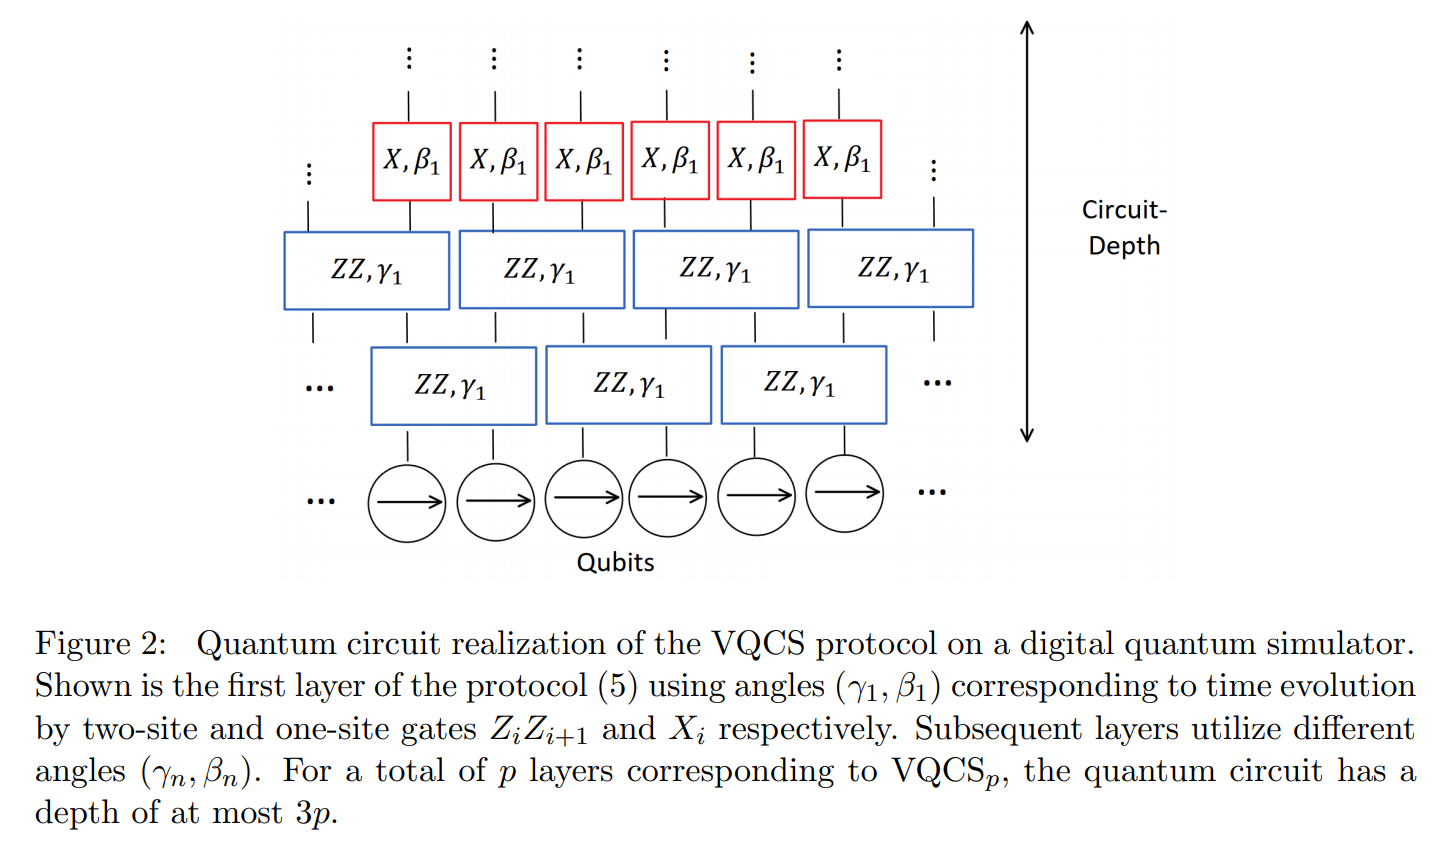
\includegraphics[scale=0.3]{vqcs}
\end{figure}
If we start in $\ket{+}$ then since the VQCS respects this symmetry, optimization of $F_p(\bm\gamma,\bm\beta)$ as $p\to \infty$ yields the GHZ state, with $\lim_{p\to \infty} F_p(\bm\gamma,\bm\beta)/L = -1$. \\


Let's see how this performs numerically. To do this, we implement the VQCS, finding numerically the optimal angles $(\bm\gamma_* \bm\beta_*)$ that minimizes $F(\bm\gamma, \bm\beta)$ (which, remember, is the energy of the system) via a search by gradient descent of the parameter space $\gamma_i, \beta_i \in [0, \pi/2)$, for system sizes $L \leq L_1 = 18$ and for $p \leq L_1/2$. Note that the for fixed $L$, a brute force search of this parameter space takes an exponentially long time $t\sim \mathcal{O}(\mathcal{M}^{2p})$ in $p$. So, we have to ensure that the total number of runs performed is large enough o ensure convergence of the search algorithm to the global minimum.  Here's the result given in the paper:
\begin{figure}[!htb]
	\centering
	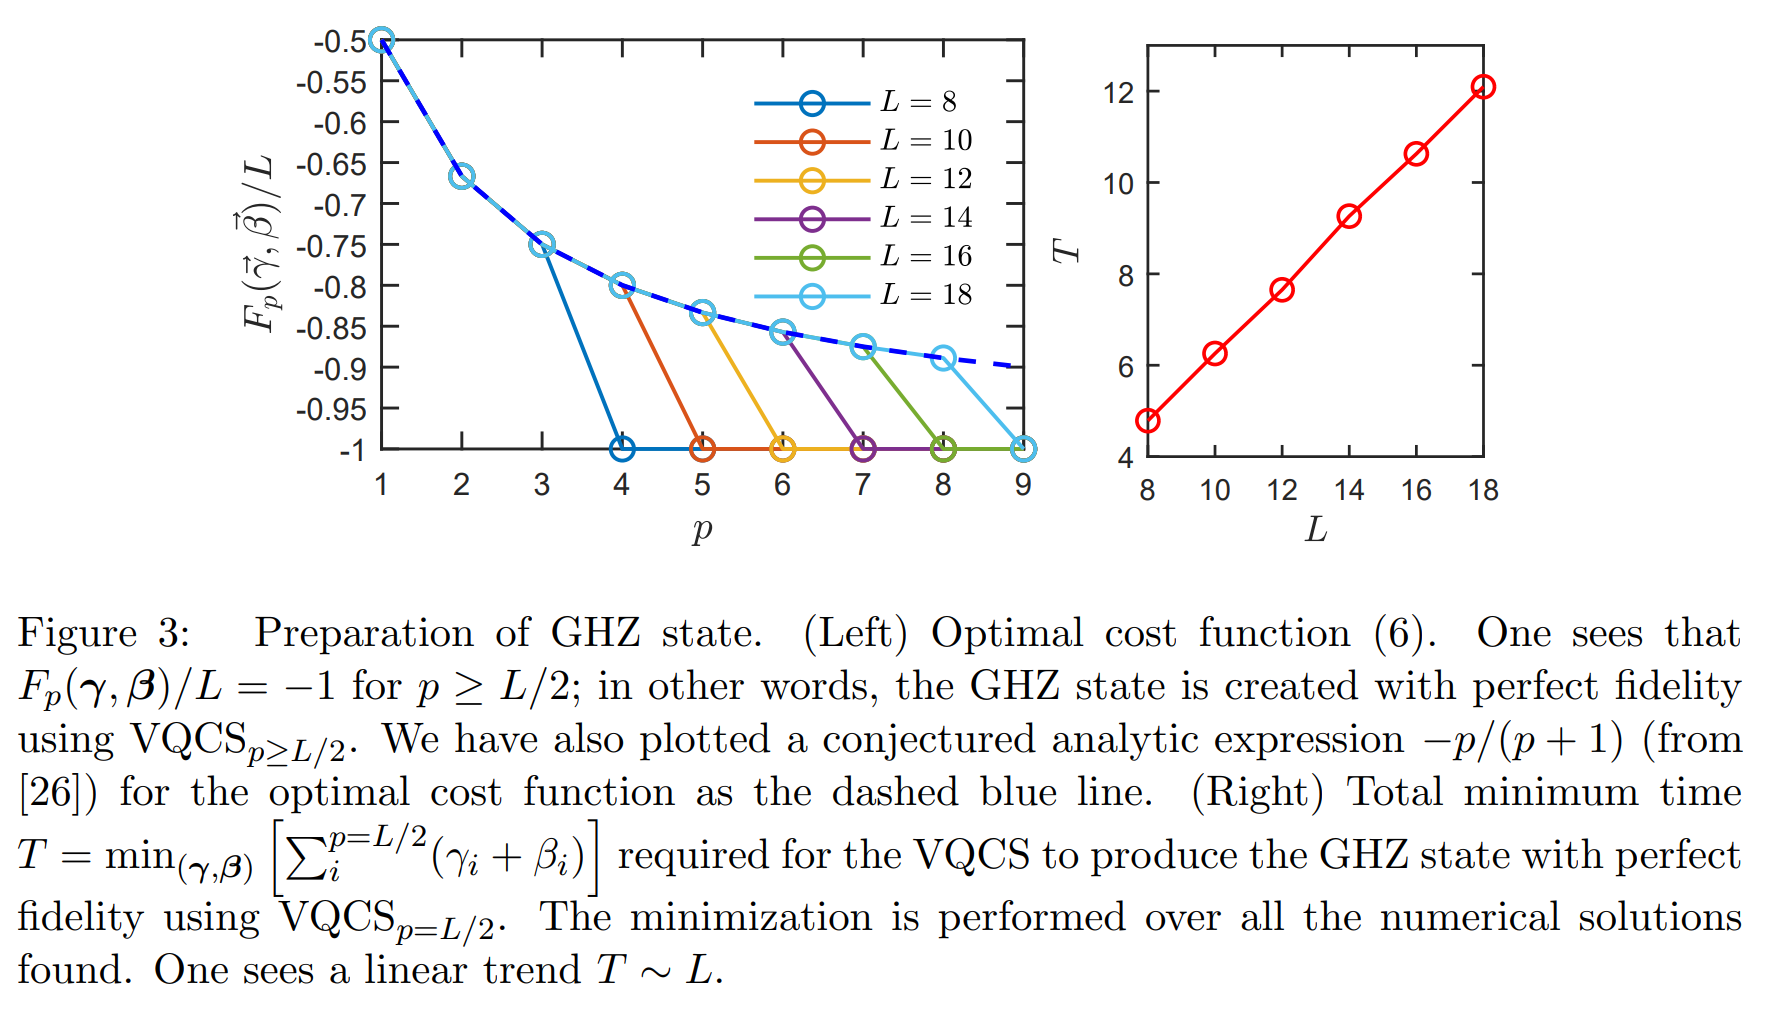
\includegraphics[scale=0.25]{ghz}
\end{figure}

The figure is quite self-explanatory so I won't go into much detail there.  We will just note that the preparation achieves perfect fidelityto machine precision. \\



Let's also note that various quantum circuits are known to also exactly prepare the GHZ state (using Hadamard and CNOT, and so on). Furthermore, experimentally, GHZ states of various sizes have been prepared with high fidelity using the Molmer-Sorensen technique in trapped ions. The VQCS is complementary in that it provides a uniform circuit that achieves the same result. 


 

\subsubsection{Critical State}

Consider the preparation of the critical state. namely the ground state of the critical 1d transverse field Ising model (TFIM) on a ring:
\begin{align}
\had_T = -\sum^L_{i=1}Z_i Z_{i+1} - \sum^L_{i=1}X_i.
\end{align}
As before, we assume the same operators $H_1 = -\sum^L_{i=1}X_i$ and $H_2 = -\sum^L_{i=1} Z_i Z_{i+1}$ as before, though now we want to minimize the new cost function $F(\bm\gamma, \bm\beta)$ using this $H_T$. In this case, we benchmark the simulation by computing the overlap $\abs{\braket{\psi_p}{\psi_t}}^2$ where the ground state of the system $\ket{\psi_t}$ is obtained (theoretically) by exact diagonalization. \\
\begin{figure}[!htb]
	\centering
	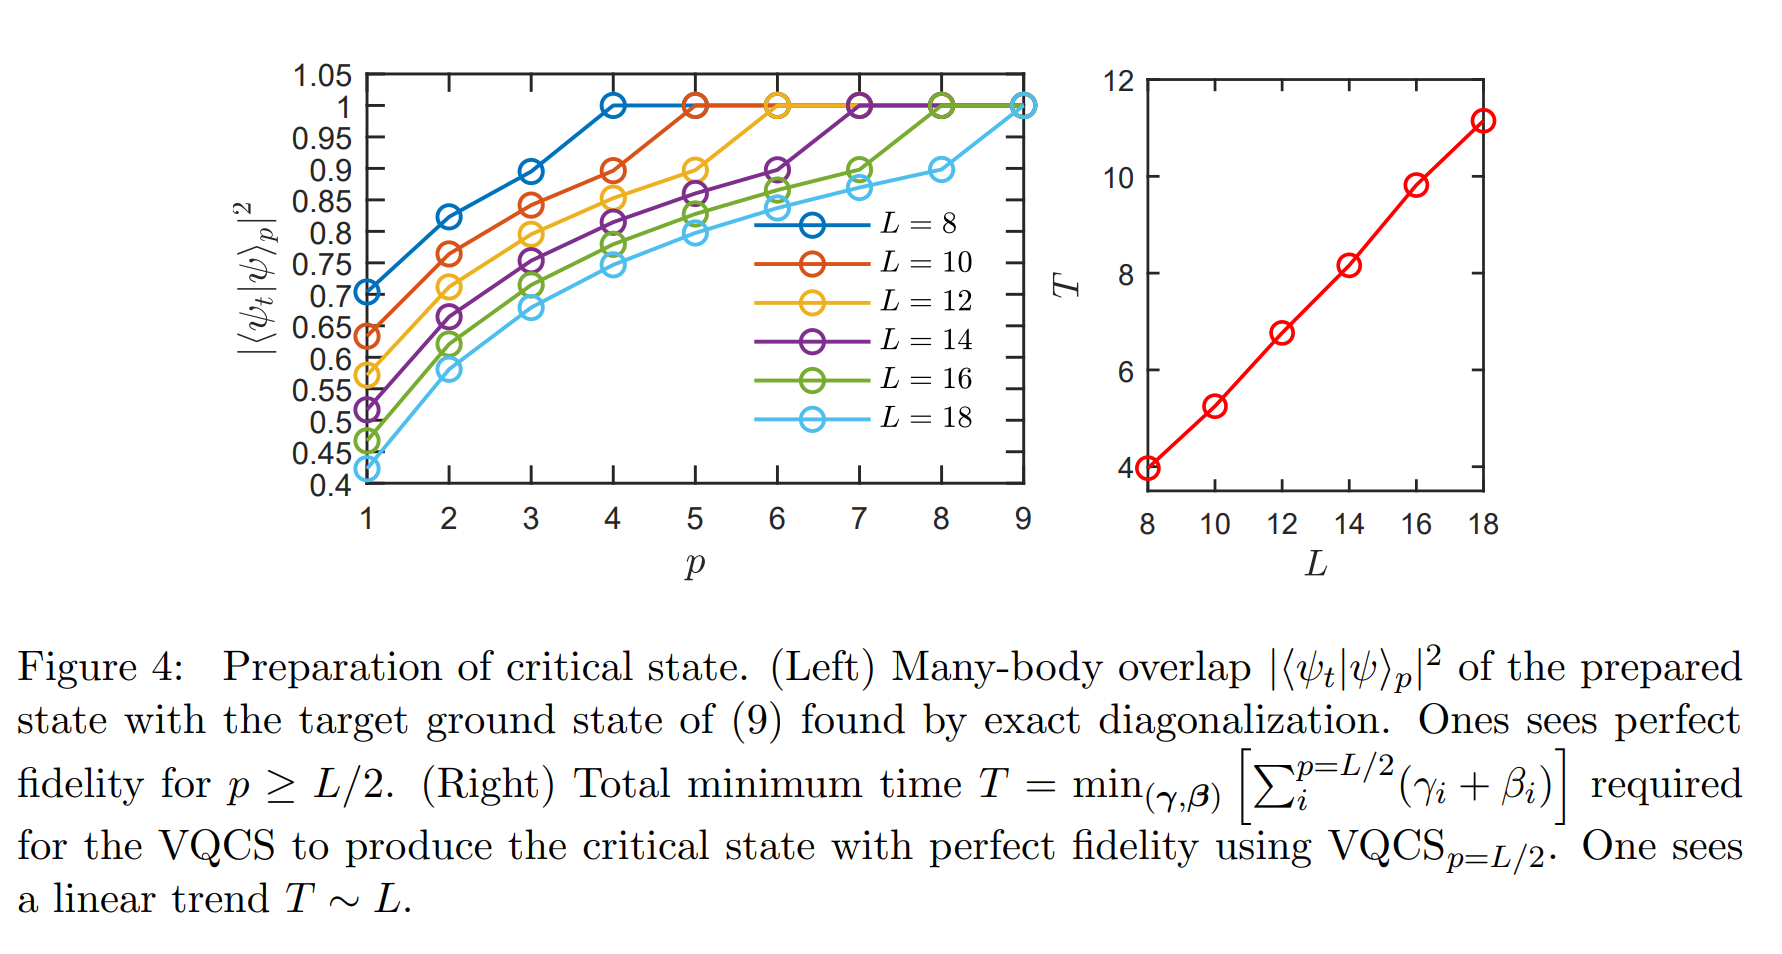
\includegraphics[scale=0.25]{critical}
\end{figure}

Once again we observe that perfect fidelity can be obtained. 





\subsubsection{Ground states of the TFIM at generic points in the phase diagram}


The perfect fidelities achieved for both the GHZ and critical cases using the VQCS for $p = L/2$ suggest that other points $g$ in the phase diagram of the TFIM 
\begin{align}
H_{\text{TFIM}} = -\sum^L Z_i Z_{i+1} - g\sum^L X_i
\end{align}
might be similarly targeted. The paper conjectures that for a 1d system of even $L$ spin-1/2s with period boundary conditions, any state produced by VQCS for arbitrary $p$ using the $H_2, H_1$ above can also be achieved perfectly by the same procedure. This would imply that it is possible to achieve the ground state of $H_{\text{TFIM}}$ at any point $g$ in the phase diagram, which in particular would cover the GHZ and critical cases.   \\

Let's note that while perfect fidelities achieved (to numerical precision) suggest that an analytic understanding may be possible. However, while the model and unitary gates can be mapped to free fermions, the minimization of the VQCS cost function maps to a nonlinear optimization problem involving an extensive number of variables, which is highly nontrivial. s


















\subsubsection{Ground state of the Toric code}

This is complicated, so we'll come back to this later. The upshot is that the VQCS procedure also works well here (perfect fidelity and so on) with runtime increasing linearly with $L$, which something we also saw before.\\

One thing to note here is just that Toric code are those with Hamiltonians with four interacting neighboring qubits.  For example, the Hamiltonian looks like 
\begin{align}
\had = -\sum^L_i \sum^L_j \sigma^x_{i,j+1}\sigma^y_{i+1,j+1}\sigma^x_{i=1,j}\sigma^y_{i,j}.
\end{align}
The Toric code is an example of topologically-ordered quantum state. Toric codes can describe really exotic behaviors that are too advanced for our guide here. For more detail, consult Wikipedia. 

\subsubsection{Ground state of AFM Heisenberg chain}


Here we consider targeting the ground state of the AFM spin-1/2 Heisenberg chains with open boundary conditions,
\begin{align}
\had_T = \sum^{L-1}_{i=1}\bm{S}_i \cdot \bm{S}_{i+1}.
\end{align}
Heres we use
\begin{align}
H_1 = \sum^{L/2-1}_{i=1} \bm{S}_{2i} \cdot \bm{S}_{2i+1}, \quad H_2 = \sum^{L/2}_{i=1} \bm{S}_{2i-1} \cdot \bm{S}_{2i}, 
\end{align}
whilst evaluating the energy as the cost function. Note that the initial state is now the product state of Bell pairs $\bigotimes_i (1/\sqrt{2})\lp \ket{\uparrow\downarrow} + \ket{\downarrow\uparrow} \rp_{2i-1,2i}$, and that angles can be restricted to $\gamma,\beta \in [0,2\pi)$.
\begin{figure}[!htb]
	\centering
	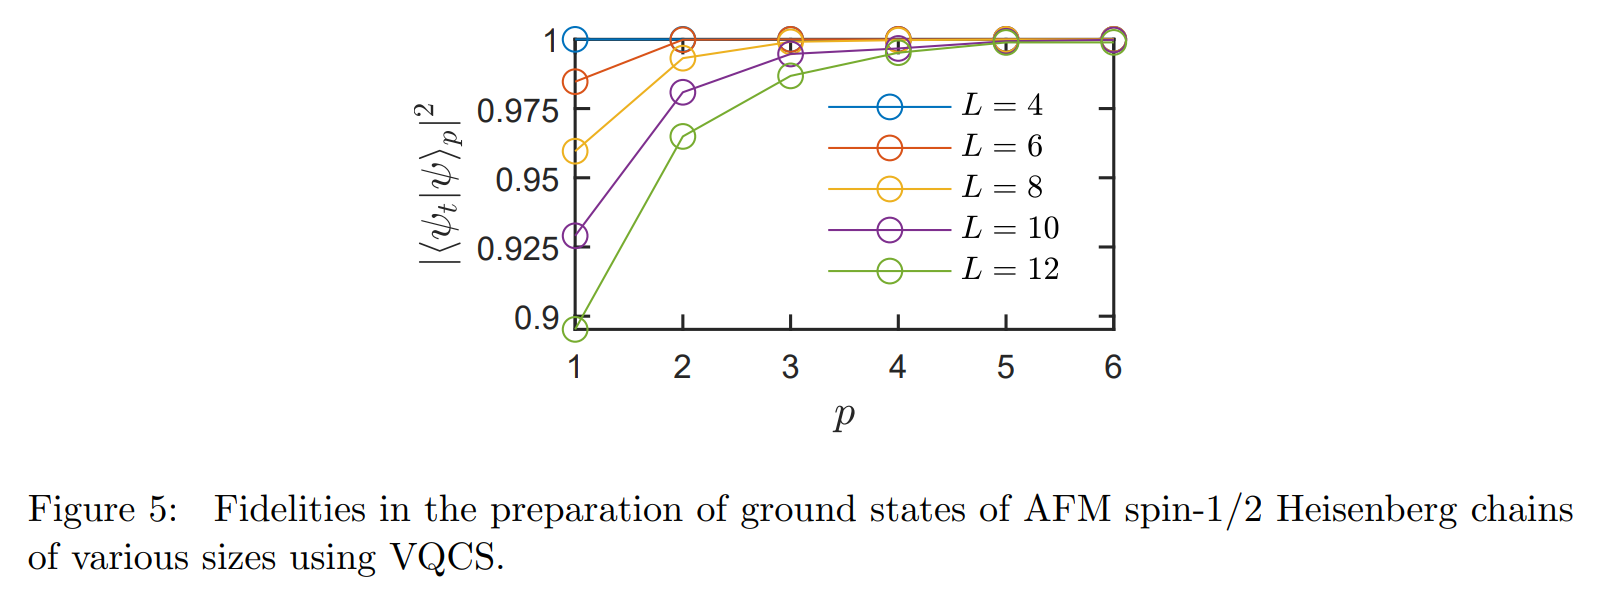
\includegraphics[scale=0.3]{afm}
\end{figure}

In this case, while the preparation of the ground states is generically not perfect for any finite $p$, the many-body fidelities are already very good for very low $p$'s, at least for small system sizes (small $L$). This illustrates the utility and generality of VQCS in preparing non-trivial quantum states. 





%\subsection{Conclusions}
%
%
%\subsection{Appendix}
%
%\subsubsection{Optimal angles for preparing GHZ state at $p=L/2$}
%\subsubsection{Explicit nonuniform unitary circuit for preparing the GHZ state}
%\subsubsection{Energy optimization plot and optimal angles for preparing critical state at $p=L/2$}
%\subsubsection{A Conjecture and Numerical Support}
%\subsubsection{Numerical verification of preparation of Toric code ground state}
%\subsubsection{Effect of errors on VQCS state preparation}







\newpage


\section{Cluster States \& Measurement-based QC}


In this section we look at concepts such as \textit{cluster states} and \textit{measurement-based quantum computation} as introduced in this \href{https://arxiv.org/pdf/quant-ph/0504097.pdf}{\underline{paper}} by M. Nielsen. I will assume familiarity with the basics of the quantum circuit model and go straight to the cluster state model.

We will explain the cluster state model of quantum computation, and explain how cluster states can e used to efficiently simuate quantum circuits. 

\subsection{How it works}


A cluster-state computation begins with the preparation of a special entangled many-qubit quantum state, known as the \textit{cluster state}, followed by an adaptive sequence of single-qubit measurements, which process the cluster, and finally read-out of the computation's result from the remaining qubits. \\

The term \textit{cluster state} refers not to a single quantum state, but rather a class of quantum states. To any graph $G$ on $n$ vertices we can define an associated $n$-qubit cluster state, by first associating to each vertex a corresponding qubit, and then applying a graph-dependent preparation procedure to the quits. For example, this graph represents a six-qubit cluster state:
\begin{figure}[!htb]
	\centering
	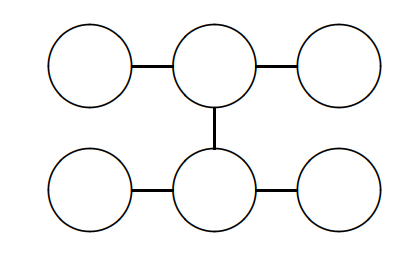
\includegraphics[scale=0.3]{cluster1}
\end{figure}
The cluster state associated to the graph may be defined as the result of applying the following preparation procedure:
\begin{itemize}
	\item Prepare each of the $n$ qubits in the state $\ket{+} = (\ket{0} + \ket{1})/\sqrt{2}$.
	
	\item Applying the controlled-PHASE gates between qubits whose corresponding graph vertices are connected. Recall that the controlled-PHASE looks like
	\begin{figure}[!htb]
		\centering
		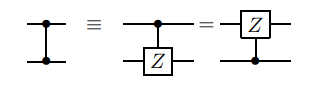
\includegraphics[scale=0.5]{cphase}
	\end{figure}
	and remember that in the first case the $Z$ gate is applied to the second qubit if the first qubit is 1. In the second case, the $Z$ gate is applied to the first qubit if the second qubit is 1. Note that if the ``dot'' in the circuit is a circle then $Z$ is applied when the controlled qubit is 0.
\end{itemize}

Because the controlled-PHASE (or controlled-$Z$) gates commute with each other, we don't worry about the order in which these gates are applied. Also, although we have described the preparation of the cluster in terms of applying quantum gates, later in the paper we briefly describe how to prepare clusters using measurement gates, and so the cluster-state model may be regarded as a truly measurement-only model of quantum computation. \\

In the original paper by Briegel, the term \textit{graph state} is used instead of \textit{cluster states}. The term \textit{cluster state} was introduced to refer to the case where the graph $G$ is a two-dimensional square lattice. This is the class of states which could be used as a substrate for quantum computations. The term \textit{graph state} refers to states associated with more general graphs $G$. In any case, we will stay with the term \textit{cluster state} for now, for consistency. \\


Once the cluster state is prepared, (note that the cluster state has two components: the vertices of qubits and edges of operators) the next step in the computation is to perform a sequence of \textit{processing measurements} on the state. These measurement satisfy:
\begin{itemize}
	\item They are single-qubit measurements
	\item The choice of measurement basis may depend on the outcomes or earlier measurements, i.e., feedforward of classical measurement results is allowed
	\item Measurement results may be processed by a classical computer to assist in the feedforward, so that choice of the basis my be a complicated function of earlier measurement results. 
\end{itemize}

Note that for the cluster state computation to be efficient we must constrain the classical computation to be of polynomial size. \\


There are two ways to define the output of the cluster-state computation:
\begin{itemize}
	\item We can define the output in terms of the \textit{quantum state} resulting from the computation. This is the quantum state of the qubits which remain when the sequence of processing measurements has terminated. 
	
	\item We can also define in terms of the the set of \textit{read-out measurements}, a sequence of single-qubit measurements applied to the qubits which remain when the processing measurements are complete. In this case the output of the computation is a classical bit string. 
\end{itemize}

\begin{exmp}
	We will consider an example of a cluster-state computation to see how it might work explicitly.  
	\begin{figure}[!htb]
		\centering
		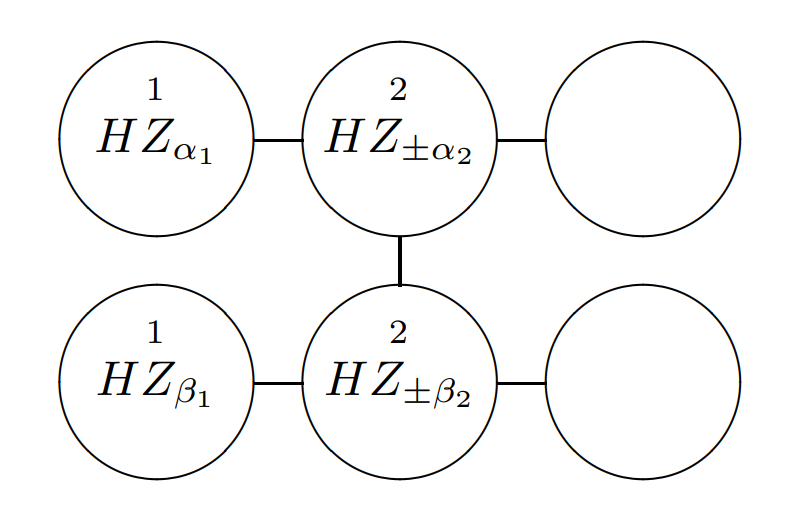
\includegraphics[scale=0.3]{cluster2}
	\end{figure}
	In this example, labels indicate qubits on which processing measurements occur, while unlabeled qubits are those which remain as the output of the computation when the processing measurements are complete. The labeled qubits are labeled with (1) a positive integer $n$ and (2) a single-qubit unitary, which we refer to as a generic unitary $U$. Here, $U = HZ_{\pm \al_{j}}, HZ_{\pm \be_j}$. \\
	
	The positive number $n$ indicates the time-ordering of the processing measurements. Qubits of the same $n$ can be measured in either order or simultaneously. The time-ordering is important, because it determines which measurement results can be fed forward to control later measurement bases. \\
	
	The unitary label $U$ indicates the basis in which the qubits is measured, denoting a rotation by the unitary $U$, following by a computational basis measurement.  In other words, a single-qubit measurement in the basis $\{  U^\dagger \ket{0} , U^\dagger\ket{1} \} $ is performed. The notation $\pm$ denotes the fact that the choice of sign depends on the outcomes of earlier measurements, in some specified manner. We will look at an explicit example later. 
\end{exmp}







 




\subsection{Simulating quantum circuits in the cluster-state model}

In this part we look at how cluster-state computation can simulate quantum circuits. The key idea underlying this example is the one-bit teleportation: 

\fig{0.5}{tele}

Here $m$ is the outcome of the computational basis measurement on the first qubit. Let's verify this. Suppose we start out with $\ket{\psi} = \al\ket{0} + \be\ket{1}$ and $\ket{+} = (1/\sqrt{2})(\ket{0} + \ket{1})$. Then the composite quantum state is given by
\begin{align}
\ket{\psi +} = \al\ket{00} + \beta\ket{11} + \al\ket{01} + \be\ket{10}.
\end{align}
A controlled-$Z$, followed by a Hadamard on the first qubit gives
\begin{align}
(\had \otimes \Id) C_Z\ket{\psi +} &= \al\ket{+0} - \be\ket{-1} + \al\ket{+1} + \be\ket{-0} \nn\\
&= \al\ket{++} + \be\ket{--}.
\end{align}
This state can be re-written as 
\begin{align}
(\had \otimes \Id) C_Z\ket{\psi +} &= \f{1}{\sqrt{2}}(\ket{0} \otimes \had \ket{\psi} + \ket{1}\otimes X \had\ket{\psi})\nn\\
&= \f{1}{\sqrt{2}}(\ket{0} \otimes X^0 \had \ket{\psi} + \ket{1}\otimes X^1 \had\ket{\psi}).
\end{align}
So the result follow. However, we can general this a bit further to get the following teleportation circuit:

\fig{0.4}{tele1}

The proof is similar. We note that $Z_\theta$ commutes with the controlled-$Z$, so the output of the circuit is the same as would have been output from the previous circuit had $Z_\theta\ket{\psi}$ been input instead of $\ket{\psi}$.  \\

What do learn from this? We see that even though the first qubit is measured, no quantum information is lost, for no matter what measurement outcome, the posterior state of the second qubit is related by a known unitary transformation to the original input $\ket{\psi}$: $\ket{\psi}$ vs. $X^m \had Z_\theta$. \\

This might seem unsurprising. However, notice that by varying the basis in which the first qubit is measured, i.e., by varying $\theta$, we can vary the unitary transformation acting on the second qubit without destroying any quantum information. 

\subsubsection{Single-qubit case}

Now, we will use this example to explain how the cluster-state computation can simulate quantum circuits. Let us explain how to simulate a single-qubit circuit of the form

\fig{0.5}{cluster3}

This looks trivial, but is very important. Here we are assuming that the qubit starts at $\ket{+}$ and single-qubit gates are of the form $\had Z_\al$ for convenience. The associated cluster-state computation used to simulate the given circuit is 

\fig{0.4}{cluster4}

Note that in order to simulate this one-qubit quantum circuit, we require 03 qubits in the cluster-state model. This will be a recurring theme in the cluster-state computation: the complexity in the quantum circuit is prepackaged into the initial quantum state, so that the complexity of the measurements is reduced. By construction, this cluster-state model is equivalent to the following quantum circuit:

\fig{0.4}{cluster5}

where we have assumed all qubits are starting out in the $\ket{+}$ state. Further, we can also equivalently delay the controlled-$Z$ between the second and third qubits to after $\had Z_{\al_1}$ to split the circuit into two parts like this:

\fig{0.4}{cluster6}

It can be readily checked that these circuits are equivalent. This can be done by thinking of the ``arrow of time'' in the cluster-state model as pointing out of the page. \\

By splitting the circuit like this, we can see that the two highlighted boxes are of the form  of the one-bit teleportation circuit that we just discussed. This means that two teleportations occur in this circuit. The first teleportation send $\ket{\psi} = \ket{+}$ to the second qubit, which has the form:
\begin{align}
\text{After 1st teleportation: } \ket{\psi_1}=   X^{m_1} \had Z_{\al_1}\ket{+}
\end{align}
as shown earlier. \\

The second teleportation sends this $\ket{\psi_1}$ to the third qubit, which has the form
\begin{align}
\text{After 2nd teleportation: } \ket{\psi_2}=  X^{m_2}  \had Z_{\pm \al_2} X^{m_1} \had Z_{\al_1}\ket{+}
\end{align}
as shown earlier. Of course, $m_1 ,m_2$ are the outputs of the measurements on the first and second qubits, respectively.\\

Observe further that feedforward can be used to choose the sign of $\pm \al_2$ so that $Z_{\pm  \al_2} X^{m_1} = X^{m_1}Z_{\al_2}$. Also, it is well-known that $\had X^{m_1} = Z^{m_1}\had$, so we can write the output as
\begin{align}
X^{m_2} \had Z_{\pm \al_2} X^{m_1} \had Z_{\al_1}\ket{+} &\to X^{m_2} Z^{m_1}\had Z_{\al_2}\had Z_{\al_1} \ket{+}\nn\\
&= X^{m_2} Z^{m_1} (\had Z_{\al_2} \had Z_{\al_1} \ket{+}) .
\end{align}
We see that, up to known Pauli matrices $X^{m_2}, Z^{m_1}$, the output is identical to the output of the circuit

\fig{0.5}{cluster3}

which we introduced earlier. \\


\noindent \textbf{Remark:} We can (easily) generalize this example to larger single-qubit circuits containing gates of the form $\had Z_{\al_j}$. Here's the general proof:
\begin{itemize}
	\item Rewrite the cluster-state computation in terms of an equivalent quantum circuit. 
	\item Reinterpret the quantum circuit as a sequence of circuits of the \textit{teleportation form}, i.e., move the controlled-$Z$'s around to make the highlighted boxes. 
	\item In the resulting expression for the output state, commute operators of the form $X^m$ all the way to the left, using feedforward to choose signs on the terms of the form $Z_{\pm \al}$ to ensure that after commutation they are of the form $Z_\al$.
	\item The result is a state which, up to known factors of Pauli matrices, is equivalent to the output of the single-qubit quantum circuit. 
\end{itemize}


\subsubsection{Multi-qubit case}
These ideas generalize to multi-qubit quantum circuits. For example, consider the quantum circuit:

\fig{0.55}{cluster7}

I claim that this quantum circuit can be simulated using the cluster-state computation

\fig{0.45}{cluster2}

We notice a (weak) pattern here. The number of qubits necessary for the cluster to simulate a 2-qubit quantum circuit is now 6. (last time it was 3 qubits to simulate a 1-qubit circuit). In any case, the proof of this equivalence follows exactly the same lines as in the single-qubit case, and is notationally more complicated. It suffices to prove this diagrammatically. To do this, we first label the qubits like so:

\fig{0.35}{cluster8}

By definition, the cluster state computation has the following associated quantum circuit:

\fig{0.35}{cluster9}

Since the controlled-PHASE/controlled-$Z$ can be moved around (as we have argued before), this circuit is equivalent to

\fig{0.35}{cluster10}

Based on the highlighted boxes, we can see that this quantum circuit is equivalent to 

\fig{0.35}{cluster11}

With this we're done. \\

So, summing p, we have shown how the cluster-state model of computation can be used to efficiently simulate any quantum circuit whose inputs are all $\ket{+}$ states, and whose gates are either controlled-PHASE gates, or gates of the form $\had Z_\al$. This set of resources is \textit{universal} for quantum computation, and thus the cluster-state model is capable of efficiently simulating any quantum circuit. \\

Conversely, it is straightforward to see that any cluster-state model can be efficiently modeled by a quantum circuit model, and thus the two models are computationally equivalent. 













\subsection{Properties}

Now we discuss some properties of the cluster-state model of computation. We address two simple but fundamental questions about cluster states, and present some progress on answering these questions:

\begin{itemize}
	\item Can cluster states arise as ground states of some naturally occurring Hamiltonian? 
	
	\item What general properties of a quantum state enable it to serve as a substrate for quantum computation, in a manner similar to the cluster state? 
\end{itemize}




\subsubsection{Cluster states and ground states of many-body quantum systems}


We won't focus too much on the details in this section. I will just focus on the fact that cluster states are in general not ground states of naturally/realistic Hamiltonians. However, this does not mean we can't prepare them in a lab or on a digital quantum computer. In particular, clusters arising in simulations of non-trivial multi-qubit quantum circuits cannot be non-degenerate ground states. \\

The question of obtaining a general classification of which clusters satisfy these conditions is still open. It would be of great interest to develop a general understanding of which clusters can and cannot arise as ground states of physically reasonable Hamiltonians.  


\subsubsection{Linearly assembled quantum states can be efficiently simulated on a quantum computer}


Now we look at what makes cluster states useful substrates for quantum computation. We will show that spatial dimension plays a role, proving that quantum states which can be linearly prepared in one dimension can always be simulated efficiently on a classical computer, and thus are \textbf{not} useful for quantum computation. 

\begin{defn}[Linearly preparable]
	A linearly preparable quantum state $\ket{\psi}$ can be prepared using a circuit of the form of cascading sequence of two-quit quantum gates applied to some product starting state like so:
	
	\fig{0.35}{linear}
	
	We note that the two-dimensional cluster states we have been using are not linearly preparable:
	
	\fig{0.45}{cluster1}
	
\end{defn}
	
Now, suppose we perform a sequence of quantum measurements on a linearly assembled quantum state, e.g.,
	
\fig{0.3}{linear1}
	
where earlier measurement results may be used to control later measurement bases. Note that the measurement gates above may be in any single-qubit basis, not just the
computational basis. This is equivalent to the following circuit
	
\fig{0.3}{linear2}
	
We claim that we can use a classical computer to simulate such a circuit.
\begin{itemize}
	\item First, we consider the result of applying $U_{12}$ to $\ket{00}$ and compute the probabilities fo the measurement on qubit 1.
		
	\item We then sample from this distribution to produce a posterior state for qubit 2, which is used as an input for $U_{23}$. 
		
	\item Then, repeat this cycle of computing probabilities, sampling, and computing posterior states.
		
	\item To make the overall result accurate, it suffices to carry out computations to $\mathcal{O}(\log (1/n))$ bits of precision, and thus the entire computation can be carried out using $\mathcal{O}(n \log^c(1/n))$ operations, where $c$ is some constant arising from the need to multiply floating point numbers. 
\end{itemize}

The point here is that efficient classical simulation of such a computation can be performed.\\

An elaboration of this argument takes care of the case where we measure the qubits in some other order, for example: 

\fig{0.3}{linear3}

I won't go into the details here. \\


This efficient classical simulation procedur can easily be generalized to a sequence of measurements performed in any order on the qubits including adaptive orderings. It is also straightforward to extend these resuts to some simple variants on the linear topology, including rings, and a small number of interlinking rings. \\


It remains an interesting open problem to determine what class of states can be used as
a substrate for quantum computation. The examples in this subsection indicate that the
geometry underlying the preparation procedure plays a key role.
	



	
















\newpage

\section{Mesurement-based quantum computing: Jozsa}

This \href{https://arxiv.org/pdf/quant-ph/0508124.pdf}{\underline{paper}} by Richard Jozsa introduces two schemes of measurement-based quantum computation: the oe-way quantum computer (1WQC) (or equivalently the cluster state model) and the teleportation quantum computation (TQC).  The former was formulated by Briegel et al while the latter by Gottesman, Chuang, Nielsen, and Leung. While I want to discuss both models, we will want to read this paper with a focus on \textit{cluster state computation}. It turns out that there's a close relationship between these models, so it's probably useful to know both. But we'll see how much we want to understand teleportation-based QC. \\

Remember that in the formalism of measurement based quantum computation we start with a given fixed entangled state of many qubits and perform single-qubit measurements to designed qubits in designated bases. The choice of basis for later
measurements may depend on earlier measurement outcomes and the final result of the computation is determined from the classical data of all the measurement outcomes. This is in contrast to the more familiar gate array model in which computational steps are unitary operations.\\

In contrast to unitary evolution, measurements are irreversibly destructive, involving much loss of potential information about a quantum state’s identity. Thus it is interesting, and at first sight surprising, that we can perform universal quantum computation using only measurements
as computational steps. These ``measurement based'' models are especially interesting for fundamental issues: they have no evident classical analogues and they offer a new perspective on the role of entanglement in quantum computation. 


\subsection{Review}

It's never a bad time to review the ubiquitous gates used in this QC. First, the Pauli matrices:
\begin{align}
I = \Id, \quad X = \begin{bmatrix}
0 & 1 \\ 1 & 0
\end{bmatrix},\quad Z = \begin{bmatrix}
1 & 0 \\ 0 & -1
\end{bmatrix},\quad iY = ZX = \begin{bmatrix}
0 & 1 \\ -1 & 0
\end{bmatrix}.
\end{align}
$\oplus$ denotes addition mod 2. The controlled-$NOT$ gate is given by 
\begin{align}
CX\ket{i}\ket{j} = \ket{i}\ket{i\oplus j}.
\end{align}
The controlled-PHASE is given by
\begin{align}
CZ\ket{i}\ket{j} = (-1)^{ij}\ket{i}\ket{j}.
\end{align}
Note that in contrast to the $CX$ gate, $CZ$ is symmetrical in two qubits. The Hadamard is given by
\begin{align}
\had = \f{1}{\sqrt{2}}\begin{bmatrix}
1 & 1 \\ 1 & -1
\end{bmatrix}
\end{align}
with the basis states $\ket{\pm}$. The Bell basis states are
\begin{align}
&\ket{B_{00}} = \f{1}{\sqrt{2}}(\ket{00} + \ket{11}) = I\otimes I \ket{B_{00}}\nn\\
&\ket{B_{01}} = \f{1}{\sqrt{2}}(\ket{01} + \ket{10}) = X\otimes I \ket{B_{00}}\nn\\
&\ket{B_{10}} = \f{1}{\sqrt{2}}(\ket{00} - \ket{11}) = Z\otimes I \ket{B_{00}}\nn\\
&\ket{B_{11}} = \f{1}{\sqrt{2}}(\ket{10} - \ket{10}) = iY\otimes I \ket{B_{00}}\nn\\
\end{align}
Succinctly, we have
\begin{align}
\ket{B_{cd}} =Z^c X^d \otimes I \ket{B_{00}}.
\end{align}
The maximally entangled states is given by
\begin{align}
\ket{\had} = \f{1}{\sqrt{2}}(\ket{0+} + \ket{1-}) = \f{1}{\sqrt{2}}(\ket{+0} + \ket{-1}) = CZ\ket{++}.
\end{align}





\subsection{Adaptive Measurements}

In this section we introduce some identities that are useful for us when we perform adaptive measurements. Our goal is to elaborate on how one makes \textit{adaptive measurements}, i.e., make measurements on some basis such that the state acquired by the subsequent qubit is ``nice.'' Here, ``nice'' means that we can use known rules of Pauli propagation (e.g. $HXH = Z$) or commute things around, and so on.\\ 


Here's the idea. Suppose we wish to perform arbitrary sequences of gates from a universal set by measurements. For simplicity, consider 1-qubit gates: to perform $\dots U_3 U_2 U_1\ket{\psi}$ we successively teleport the three gates but instead of the described result we get something like $\dots P_3 U_3 P_2 U_2 P_1U_1\ket{\psi}$ where $P_i$ are the Pauli operators depending on the measurement outcomes To deal with this awkwardness we introduce \textit{adaptive choices} of measurements. This was introduced in the previous section as ``feeding forward the result of the last measurement into the next measurement.'' \\

Let us assume that all 1-qubit operations are $x$ or $z$ rotations. The following Pauli propagation relations are easily verified:
\begin{align}
R_x(\theta)X = XR_x(\theta), \quad R_x(\theta)Z = ZR_x(-\theta), \quad R_Z(\theta)X=XR_z(-\theta), \quad R_z(\theta)Z = ZR_z(\theta).
\end{align}
These make sense: rotating in the same axis commutes. Rotating in the different axes don't commute. To swap the order of rotation, we also have to flip the direction of the rotation, so that it undoes the parity change. \\

We also have
\begin{align}
W(\theta)X = ZW(-\theta), \quad W(\theta)Z = XW(\theta)
\end{align}
where
\begin{align}
W(\theta) = HP(\theta) = \f{1}{\sqrt{2}}\begin{bmatrix}
1 & 1 \\  1 & -1
\end{bmatrix}\begin{bmatrix}
1 & 0 \\ 0 & e^{i\theta}
\end{bmatrix} = \f{1}{\sqrt{2}}\begin{bmatrix}
1 & e^{i\theta} \\ 1& e^{-i\theta}
\end{bmatrix}.
\end{align}

Now, suppose we want to do $R_z(\be)R_x(\al)\ket{\psi}$. Now, there's a lot of short-hand notation here, but the important thing we have to keep in mind is that $\ket{\psi}$ is actually initially adjoined by $\ket{B_{00}} = (1/\sqrt{2})(\ket{00} + \ket{11})$. With this, it makes sense to make a Bell measurement on the qubit pair and get teleportation (in the Jozsa sense). Consider the object we want to evaluate:

\fig{0.3}{bell-measure}

After the first unitary, the state of interest becomes $R_x(\al)\ket{\psi}$. A Bell measurement gives outcomes $a,b$ and returns the teleported state $Z^a X^b R_x(\al)\ket{\psi}$ where $a,b\in \{0,1\}$. The proof of this are everywhere (and quite easy), so let's not worry about the details. \\

Now we notice that commuting $Z^a X^b$ to the left through $R_z(\be)$ causes $\beta$ to change to $(-1)^b \beta$. So, if instead of $R_z(\beta)$ we next applied the Bell measurement for $R_z((-1)^b \beta)$ then 
\begin{align}
R_Z((-1)^b \beta) Z^a X^b R_x(\al)\ket{\psi} = Z^a R_z((-1)^b\beta)X^b R_x(\al)\ket{\psi}= Z^a X^b R_z(\beta)R_x(\al)\ket{\psi}
\end{align}
as wanted. Suppose this second measurement with basis adapted to measurement outcome $b$ has an outcome $c,d$ say, and the state is now $Z^{a+c} X^{b+d} R_z(\beta) R_x(\al) \ket{\psi}$. Continuing in this way, adapting measurement bases to earlier measurement results we get
\begin{align}
\dots X_2^{m_2}Z_2^{n_2}X_1^{m_1}Z_1^{n_1} \text{(the correct wanted U)} \ket{\psi}.
\end{align}
Here $\ket{\psi}$ is a state of many qubits and $X_i, Z_i$ are Pauli operators on the $i$th qubit. The indices $m_i,n_i$ are accumulations (sum mod 2) of measurement outcomes. \\

The same idea applies to the 2-qubit gate $CZ$ too where the situation is even better. We have the propagation relations:
\begin{align}
CZ(Z\otimes I) = (Z\otimes I)CZ,\quad CZ(X\otimes I) = (X\otimes Z) CZ.
\end{align}
Thus we can propagate Pauli operators through $CZ$ while keeping $CZ$ the same, so no basis adaption is required.\\

If $U$ is a total unitary effect of a gate array on a multi-qubit state $\ket{\psi}$ then using the above methods we are able to generate a state of the form $\dots X_2^{m_2}Z_2^{n_2}X_1^{m_1}Z_1^{n_1} U \ket{\psi}$. In a quantum computation we finally measure at least some qubits of $U\ket{\psi}$ in the $Z_i$ bases $\{ \ket{0}, \ket{1} \}$. Now, notice that $Z_i^{n_i}$ has no effect on the measurement outcomes (only phases are shifted) and $X_i^{m_i}$ requires only some simple re-interpretation of the output results (since all $X$ does is flipping bits). This means we simple need to reinterpret measurement outcome $k_i \in \{0,1\}$ as $k_i \oplus m_i$ where $m_i \in \{0,1\}$ is the exponent of the corresponding $X$ Pauli matrix. 





\subsection{Cluster-state computation/1WQC}

We just looked at this model in the previous section. However, in this section we will go into a little more detail. Remember that this model was introduced by Raussendorf and Briegel. The model starts with a 2D grid of $\ket{+}$ states, followed by applications of $CZ$ to each nearest neighbor pair in vertical and horizontal directions. The $CZ$'s commute so they can be applied in parallel, as a process of constant quantum depth. The resulting state is an entangled states of many qubits, called a \textit{cluster state}.

\fig{0.3}{jozsa1}

As we have seen, any quantum gate array can be implemented as a pattern of 1-qubit measurements on a sufficiently large 2D cluster state. The only measurements used are in the bases $M_z = \{\ket{0}, \ket{1}\}$ and $M_\theta = \{ \ket{0} \pm e^{i\theta}\ket{1} \}$ for some $\theta$. $\theta = 0$ corresponds to the $X$ basis measurements $\{ \ket{+}, \ket{-}   \}$. Measurement outcomes are always labeled 0 or 1 and they are always uniformly random.  \\

Also, as we have seen before, quantum gates are implemented only up to known Pauli correction matrices $X^a Z^b$ where $a,b$ depend on the measurement outcomes. Recall that this is due to teleportation. In the 1WQC literature, these are called the \textit{bi-product Pauli operators}. Of course, the quantum computation is ``one way'' in the sense that the initial resource of the pure cluster state is irreversibly degraded as the computation proceeds in its layers of measurement. 

\begin{exmp}
	This first example is take from this \href{https://arxiv.org/pdf/quant-ph/0301052.pdf}{\underline{paper}} by Briegel et al. For this example, we look at measurement patterns for 1-qubit gate (where a 1-dimensional cluster state suffices, as we have seen). \\
	
	We know that any 1-qubit unitary $U$ can be expressed as a three alternating rotations:
	\begin{align}
	U = R_x (\zeta)R_z(\eta)R_x(\xi),
	\end{align}
	for some $\zeta, \eta, \xi$ where of course 
	\begin{align}
	R_x(\theta) = e^{-i\theta X}, \quad R_y(\theta) = e^{-i\theta Y}, \quad R_z(\theta) = e^{-i\theta Z}
	\end{align}
	are rotation matrices (in the Bloch sphere). This is quite intuitive, so I won't explain why this is the case. Now, to apply $U$ to $\ket{\psi}$ by the 1WQC we start with $\ket{\psi}$ in a line with $04$ $\ket{+}$ qubits like this:
	
	\fig{0.3}{rotate}
	
	Remember that because there are 3 total rotations, we will need four $\ket{+}$ ``ancillary'' qubits. Next, entangle all neighboring pairs with $CZ$ gates and subsequently measure qubits $1,2,3,4$ adaptively in the bases shown in the figure. It may be shown that qubit 5 acquires the state $X^{s_2 + s_4} Z^{s_1 + s_3} U\ket{\psi}$, where $s_i$ is the outcome of the measurement on qubit $i$. \\
	
	We won't worry about the details of this example now, for we will return to this paper by Briegel et al later. But the idea is this. Recall that in the teleportation circuit we have something like
	
	\fig{0.3}{tele}
	
	where a rotation by $Z_\al$ gives a state of the form $X^m \ket{\phi}$. By a similar argument, because $HXH = Z$, we can argue that a rotation by $X_\al$ gives a state of of the form $Z^m$. This means that after the first measurement in the $X$ basis, the resulting state is going to be $Z^{s_1}$. Next, we have a rotation by $R_z$, so the next factor, roughly speaking, is going to be $X^{s_2}$, and so on. Of course, the reality is that commutation rules also dictate which power goes where in the bi-product operator. So, a careful check is necessary. In any case, we'll come back to this in the Briegel's paper, which is a more mathematically rigorous approach to all of this. 
\end{exmp}


\begin{exmp}
	In this example we consider a simpler pattern:
	
	\fig{0.3}{fig6}
	
	This is more familiar to us at this point. Again, by exchanging the role of $Z$ and $X$ between our previous examples and this one, we can see that qubit 3 acquires the state $Z^{s_1}X^{s_2}\ket{\psi}$ (remember, this is just teleportation). The two $X$ measurements may be done in parallel but we can also consider this process as a sequence of two identical steps as we have seen: given a state $\ket{\psi}$, adjoint this to $\ket{+}$, entangle them with $CZ$ and then $X$-measure the first qubit, giving an outcome $s \in \{0,1\}$. Qubit 2 is then left in the state $X^s \had \ket{\psi}$. This means the two step chain ends up in the state
	\begin{align}
	(X^{s_2}\had )(X^{s_1}\had)\ket{\psi} = X^{s_2}Z_{s_1}\ket{\psi}.
	\end{align} 
	where we have used the fact that $\had X \had  = Z$. 
\end{exmp}



\begin{exmp}
	Here we look at a single step operation for the general measurement basis $M(\theta)$.
	
	\fig{0.3}{fig7}
	
	The state $\ket{\psi}$ and $\ket{+}$ are entangled by the $CZ$. Measuring the first qubit in the basis $M(\theta) = \{ \ket{0} \pm e^{i\theta}\ket{1} \}$ leaves qubit 2 in the state $X^{s_1}W(-\theta)\ket{\psi}$. Here,
	\begin{align}
	W(\theta) = HP(\theta) = \f{1}{\sqrt{2}}\begin{bmatrix}
	1 & 1 \\  1 & -1
	\end{bmatrix}\begin{bmatrix}
	1 & 0 \\ 0 & e^{i\theta}
	\end{bmatrix} = \f{1}{\sqrt{2}}\begin{bmatrix}
	1 & e^{i\theta} \\ 1& -e^{i\theta}
	\end{bmatrix}.
	\end{align}
	Let's check this to make sure we're still on track. According to the circuit, we first have a $CZ$ between $\ket{\psi} = \al\ket{0} + \be\ket{1}$ and $\ket{+}$. This gives a new state
	\begin{align}
	CZ\ket{\psi+} &= CZ\f{1}{\sqrt{2}}\lb \al\ket{00} + \al\ket{01} + \be\ket{10} + \be\ket{11} \rb\nn\\
	&= \f{1}{\sqrt{2}}\lb \al\ket{00} + \al\ket{01} + \be\ket{10} - \be\ket{11} \rb.
	\end{align}
	To check that after measuring in the basis $M(\theta) = \{\ket{0} \pm e^{i\theta}\ket{1} \}$ we get $X^{s_1}W(-\theta)\ket{\psi}$ it suffices to check that 
	\begin{align}
	CZ\ket{\psi+} = (\ket{0} + e^{i\theta}\ket{1})X^0W(-\theta)\ket{\psi} + (\ket{0} - e^{i\theta}\ket{1})X^1 W(-\theta)\ket{\psi}.
	\end{align}
	This is not hard to check, so I'll leave this to the reader. The point is to show that qubit 2 acquires the state $X^{s_1}W(-\theta)\ket{\psi}$. \\
	
	The point of this example is to show that if we are not concerned with issues of parallelizability then any 1D measurement pattern may be viewed as a sequential application of the process this example, measurements in the $M(\theta)$ basis, applied repeatedly. \\
	
	This shows that the unitary operation $W(\theta)$ plays a fundamental role in 1WQC/cluster state computation. For instance, in the previous example, 
	
	\fig{0.3}{rotate}
	
	we can reorder all operations as follows: (entangle 12, measure 1), (entangle 23, measure 2), and so on. This is because the 12-entangling operation and first measurement both commute with all subsequent entangling operations and measurements. Of course, the basis $M(\theta)$ is identically $X$ if $\theta = 0$.
\end{exmp}


From there examples, we can concatenate gates. Suppose we wish to apply $U_1$ then $U_2$ to some input $\ket{\psi}$. Now, measurement pattern 1 for $U_1$ gives an output that is the input for $U_2$. But all measurements in pattern 1 commute with all entangling operations of pattern 2 (recall we can move things the entangling and measurement 1 around in the previous section). So, we can apply all entangling operations for both patterns first, to get a longer single cluster state and then apply the measurements.\\


Finally, we can eliminate the input state $\ket{\psi}$ altogether, to get a formalism based entirely on a starting state that is a fully standard cluster state (or slightly longer length). This is because we can implement any 1-qubit unitary $U$, we can take out input starting state to be $\ket{+}$ and prefix the desired process with an initial measurement pattern for a unitary operation that takes $\ket{+}$ to $\ket{\psi}$.\\

This 1D formalism may be generalized using 2D cluster grids to incorporate 2-qubit gates. For universal computation it suffices to be able to implement just the $CZ$gate in addition to 1-qubit gates. For example:

\fig{0.3}{fig8}

The dots denote the $\ket{+}$ states and connecting lines denote $CZ$ applications between the dots. If the measurement pattern shown on the right is applied at the sites, the only the unmeasured sites are of interest and contain $(P_1 \otimes P_2)CZ\ket{\psi_{in}}$ where $P_1 \otimes P_2$ is a Pauli operation that depends on the measurement outcomes. 


\subsubsection{The Role of $Z$ measurements}

Measurement patterns for general gate arrays, which are implemented on a sufficiently large 2D cluster, will general have extraneous sites not used in the measurement patterns. $Z$-measurements are used to delete such extraneous sites. To see how this works, we consider two examples. 

\begin{exmp}
Consider the following cluster:

\fig{0.45}{fig9}

This has quite an irregular shape. Suppose we only want to use sites $1,2,3$, i.e., we want to delete site $A$. Consider $Z_A$, a $Z$ measurement at site $A$, with outcome $k_A$. To see its effect we need to write down what the state resulting from figure 9 is. Now, measurement $Z_A$ commutes with $CZ_{12}$ and $CZ_{23}$. However, 
\begin{align}
CZ_{A2}\ket{++} = \ket{0+} + \ket{1-}.
\end{align}
So, after the $Z_A$ measurement (with outcome $k_A$) the sites $1,2,3$ contain $\ket{+}\ket{(-1)^{k_A}} \ket{+}$, where $\ket{(-1)^{k_A}}$ is one of the two Hadamard basis states:
\begin{align}
\sim \begin{bmatrix}
1\mp \sqrt{2} & 1
\end{bmatrix}^\top
\end{align}
This means that the effect of the $Z_A$ measurement is to have used the Hadamard basis state $\ket{\pm} = \ket{(-1)^{k_A}}$ at site $2$ instead of the standard $\ket{+}$ and then entangle as usual. \\

So, to summarize, by applying the measurement $Z_A$, we end up with the total state $\ket{+(-1)^{k_A}+}$ at $1,2,3$, and get no more entanglement with $A$. 



\end{exmp}



\begin{exmp}
	Consider the following figure again:
	
	\fig{0.4}{fig7bis}
	
	Suppose we start with $\ket{\psi -}$ instead of with $\ket{\psi +}$ as before. Applying $CZ$, then measure $M(\theta)$ at qubit 1 for output at qubit 2. The reader can check that this is the same as (i) start with $\ket{\psi +}$, (ii) apply $CZ$, (iii) measure $M(\theta)$ on qubit 1, (iv) applying the unitary $I\otimes Z_2$. Now, since $Z_2$ commutes with $CZ$ and $M(\theta)$, we can apply $I \otimes Z_2$ before applying $CZ$ and note that
	\begin{align}
	I \otimes Z_2 \ket{\psi +} = \ket{\psi -}. 
	\end{align}
\end{exmp}



In summary, we see that the measurement $Z_A$ at site $A$ with outcome $k_A$ adds in an extra $Z^{k_A}$  Pauli correction at all neighboring sites of $A$, in addition to the usual Pauli operations arising from measurement patterns in a standard cluster state that had site $A$ absent from the start. 



\subsubsection{Summary}

To summarize the cluster state/1WQC model, we have seen that
\begin{itemize}
	\item Any quantum gate array can be translated into a pattern of 1-qubit measurements on a sufficiently large 2D cluster state.
	
	\item Choices of measurement bases are generally adaptive: possibly depending on previous measurement outcomes.
\end{itemize}


\subsection{Selected extra features: Cluster state model}

\begin{thm}
	1WQC/Cluster state model with 2D cluster states is universal for quantum computation. 
\end{thm}

\fig{0.3}{1D}

However, as we have discussed, any 1WQC/cluster state process based on only 1D cluster states can be simulated classically efficiently (in polynomial time in the number of qubits). Thus, the universality of any such model would imply that quantum computation is no more powerful than classical computation. 







\subsection{Teleportation-based QC (TQC)}
As expected, I'm not going to worry about this. 


\subsection{Relationships between TQC and Cluster State models}

... or this either. 






















\newpage




\section{Measurement-based quantum computing on cluster states: Briegel et al}
In this section we will study this \href{https://arxiv.org/pdf/quant-ph/0301052.pdf}{\underline{paper}} from the originators themselves. This paper lays out a detailed account of the cluster state model of quantum computation, which is a QC scheme that consist only of one-qubit measurements on cluster states -- a class of highly entangled states.   \\

The purpose of this paper is threefold:
\begin{itemize}
	\item Proving the universality of the cluster state model
	\item Relate quantum algorithms to graphs
	\item Prove a number of examples for the cluster state circuit models which are characteristic and of practical interest. 
\end{itemize}



\subsection{Universality of the cluster state model}


\subsection{Computational model underlying the cluster state model}


\subsection{Practical examples}









\newpage









\end{document}
